% !TEX encoding = UTF-8 Unicode
% !TEX encoding = UTF-8 Unicode
\documentclass[UKenglish]{ifimaster}  %% ... or USenglish or norsk or nynorsk
\usepackage[latin1]{inputenc}        %% ... or utf8 or applemac
\usepackage[T1]{fontenc,url}
\urlstyle{sf}
\usepackage{babel,textcomp,csquotes,ifimasterforside,varioref,graphicx,caption,nameref,caption,amssymb,framed}
\usepackage[section]{placeins}
\usepackage{amsmath,lipsum}
\setcounter{secnumdepth}{3}
\interfootnotelinepenalty=10000
\usepackage{listings}
\usepackage{color}
\usepackage{array, dcolumn, booktabs,enumitem}
\usepackage[showframe=false]{geometry}
\usepackage{changepage}
\usepackage{subfigure}
\usepackage[toc,page]{appendix}
\usepackage{blindtext}

\let\Chaptermark\chaptermark
\def\chaptermark#1{\def\Chaptername{#1}\Chaptermark{#1}}
\let\Sectionmark\sectionmark
\makeatother\newcommand{\mypm}{\mathbin{\smash{%
\raisebox{0.35ex}{%
            $\underset{\raisebox{0.5ex}{$\smash -$}}{\smash+}$%
            }%
        }%
    }%
}

\setlength{\parskip}{\baselineskip}%
\setlength{\parindent}{0pt}%

\definecolor{mygreen}{rgb}{0,0.6,0}
\definecolor{mygray}{rgb}{0.5,0.5,0.5}
\definecolor{mymauve}{rgb}{0.58,0,0.82}
\lstset{ %
  backgroundcolor=\color{white},   % choose the background color; you must add \usepackage{color} or \usepackage{xcolor}
  basicstyle=\footnotesize,        % the size of the fonts that are used for the code
  breakatwhitespace=false,         % sets if automatic breaks should only happen at whitespace
  breaklines=true,                 % sets automatic line breaking
  captionpos=b,                    % sets the caption-position to bottom
  commentstyle=\color{mygreen},    % comment style
  deletekeywords={...},            % if you want to delete keywords from the given language
  escapeinside={\%*}{*)},          % if you want to add LaTeX within your code
  extendedchars=true,              % lets you use non-ASCII characters; for 8-bits encodings only, does not work with UTF-8
  frame=single,                    % adds a frame around the code
  keepspaces=true,                 % keeps spaces in text, useful for keeping indentation of code (possibly needs columns=flexible)
  keywordstyle=\color{blue},       % keyword style
  language=Java,                 % the language of the code
  morekeywords={*,...},            % if you want to add more keywords to the set
  numbers=left,                    % where to put the line-numbers; possible values are (none, left, right)
  numbersep=5pt,                   % how far the line-numbers are from the code
  rulecolor=\color{blue},         % if not set, the frame-color may be changed on line-breaks within not-black text (e.g. comments (green here))
  showspaces=false,                % show spaces everywhere adding particular underscores; it overrides 'showstringspaces'
  showstringspaces=false,          % underline spaces within strings only
  showtabs=false,                  % show tabs within strings adding particular underscores
  stepnumber=1,                    % the step between two line-numbers. If it's 1, each line will be numbered
  stringstyle=\color{mymauve},     % string literal style
  tabsize=2,                       % sets default tabsize to 2 spaces
  title=\lstname,                   % show the filename of files included with \lstinputlisting; also try caption instead of title
  numberstyle=\tiny,
}








\title{Does Limit on Work-In-Progress (WIP) matter?}        %% ... or whatever
\author{Truls Skeie}                      %% ... or whoever 
\usepackage[
    backend=biber,
    style=authoryear-icomp,
    sortlocale=de_DE,
    natbib=true,
    url=false, 
    doi=true,
    eprint=false,
    citestyle=authoryear
]{biblatex}
% !BIB TS-program = biber

\addbibresource{lib.bib}

\begin{document}
\ififorside{}
\frontmatter{}
\maketitle{}

\chapter*{Abstract}                   %% ... or Sammendrag or Samandrag

\tableofcontents{}
\listoffigures{}
\listoftables{}
\lstlistoflistings{}

\chapter*{Preface}                    %% ... or Forord

\mainmatter{}
\chapter{Introduction}
\label{chap:intro}
This master thesis focuses on limit Work In Progress (WIP), which is one of the principles in Kanban. The focus will be to see what impact WIP limit has in a development process. In order to do so, a data set gathered by an in house software company in Norway called Software Innovation (SI) was used. SI is a Scandinavian software company that delivers Enterprise Content Management applications.

The data set had already been interpreted by another study. That study investigated Scrum vs. Kanban for SI. For interested readers the case study can be found in the article "Quantifying the Effect of Using Kanban versus Scrum: A Case Study" \parencite{Dag}. 

\section{Motivation}
In software development, processes and methods are important in order to deliver the right product on time. In software development one rarely solves two identical problems for different stakeholders. And the problems are getting bigger and more complex, which means that new processes and methods are introduced and the already existing processes and methods needs to be adapted to solve the complex problems in the most efficient ways.  The number of popular software development methods  (e.g. Extreme programming, Spiral, Scrum and Kanban) emerged in the recent years proves the assumption \parencite{gandomani2013important} \parencite{ikonen2010exploring}.

This is why this thesis will focus on software development methods, the method in each development project is such a key element. The main focus of this thesis will be the Kanban method and the principle to limit Work In Progress (WIP). In Kanban the WIP limit is used to  limit the number of tasks each developer can work on at each workflow state to prevent bottlenecks and to ensure flow of tasks through the development cycle \parencite{gandomani2013important} \parencite{ikonen2010exploring}.

There are published various literature on Kanban in software development such as "Kanban: Successful Evolutionary Change for Your Technology Business" \parencite{0984521402}, "Kanban and Scrum - making the most of both"  \parencite{Kniberg} and "Lean Software Management: BBC Worldwide Case Study" \parencite{Joyce}. Although there is various literature, there is no information on how to apply WIP limit, even though most of the experience Kanban enthusiasts agree that WIP limit is an important principle.  There is no research backing the statement.  The literature states that one should experiment with WIP limits in order to find the best WIP limit for one's case \parencite{Ikonen} \parencite{Kniberg}.

Since there is lack of available research on WIP limit my motivation is to investigate WIP limit in this thesis.

\section{Research Question}
\label{chap:RQ}
In this thesis the overall research question will be to study the effects of WIP limits for an in house software company,in particular:
\begin{itemize}
\item Does WIP limit in software development matter?
%\item See if the exist an optimal WIP limit for a given context.
\item In case how to find the optimal WIP limit?
\item Which parameters should be considered in order to optimize WIP? 
\end{itemize}


\section{Approach}
This thesis will use case study as an approach  to answer the research questions. To conduct the case study a data set from an in house software company will be used.  The data set will be evaluated at team level. SI consist of ten teams, all of them will be investigated to answer the research questions. 

The program will take the part of the analysis. The program was made for this thesis in order to transform the data set from SI into more suited. The second part of the analysis will consist of statistical analysis to compute correlation and descriptive statistic.
 

\section{Chapter overview}
\begin{description}
\item[Chapter \ref{chap:Background}: \nameref{chap:Background}:] \hfill \\  
Chapter \ref{chap:Background} introduces background information and introduces relevant concepts and methods in software development as well as information about the in house software company, Software Innovation. 
\item[Chapter \ref{chap:RM}: \nameref{chap:RM}:] \hfill \\  
Chapter \ref{chap:RM} introduces and explains the research methods used in the thesis as well as complementary information about Software Innovation and why the data set from Software Innovation is used in this thesis.  
\item[Chapter \ref{ch:DCC}: \nameref{ch:DCC}:] \hfill \\
Chapter \ref{ch:DCC} gives information about the data set and the calculations. Complementary information about how the program operates is given in as well as information about how the output data from the program is measured using statistical analysis. 

\item[Chapter \ref{ch:res}: \nameref{ch:res}:] \hfill \\
\item[Chapter \ref{ch:dis}: \nameref{ch:dis}:] \hfill \\
\item[Chapter \ref{ch:con}: \nameref{ch:con}:] \hfill \\
\end{description}




%\textbf{Chapter \ref{chap:intro}: \Chaptername:} The first chapter will consist of a section where the motivation behind this thesis is stated. A section where the research questions this thesis will address. A section how I will approach the data in order to answer the research questions.  A section that will explain how I will evaluate the data in order to answer the research question and a section where contribution will be stated.   

\chapter{Background}  
\label{chap:Background}                %% ... or Bakgrunn
In this chapter there will be a brief introduction to Waterfall (Section \ref{sec:WP}), Scrum (Section \ref{sec:Scrum}), Lean (Section \ref{sec:Lean}) and Kanban (Section \ref{sec:Kan}) with affiliated tools. The software development company Software Innovation is briefly introduced (Section \ref{sec:SI})

\section {Waterfall}
\label{sec:WP}
"The waterfall model is the classical model of software engineering. This model is one of the oldest models and is widely used in government projects and in many major companies" \parencite{munassar2010comparison}.The main goal of the waterfall model is to plan in early stages to ensure design flaws before coding is started. Since planning is so critical in the waterfall method it fits project where quality control is a major concern  \parencite{munassar2010comparison}.

The waterfall method consist of several non-overlapping stages as shown in figure \ref{fig:waterfall}. The figure is an example of the waterfall model with a life cycle of establishing system requirements and software requirements and continues with architectural design, detailed design, coding, testing and maintenance  \parencite{munassar2010comparison}. One of the main principles of the waterfall method discourages return to an earlier phase. For example returning from detailed design to architectural design. However, if returning to an earlier phase is needed, it involves costly rework. When a phase is completed, the phase requires formal review and extensive documentation development. Therefore, if something is missed out an earlier phase it is expensive to correct it later  \parencite{munassar2010comparison}


\begin{figure}[ht!]
\centering
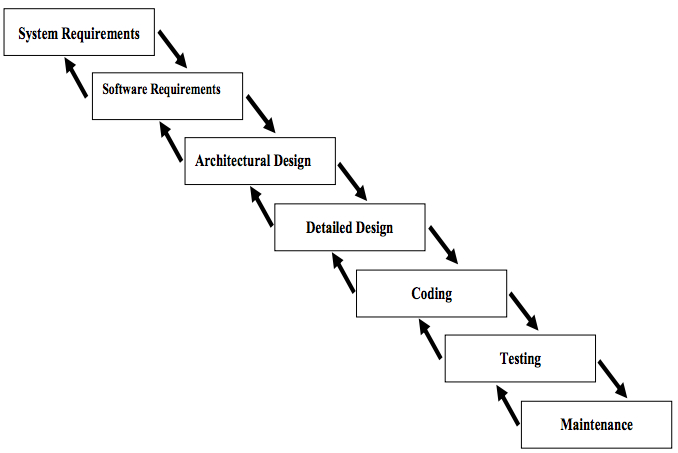
\includegraphics[scale=0.7]{Picture/waterfall.jpg}
\caption{Waterfall model}
\label{fig:waterfall} % 
\end{figure}

\section {Scrum}
\label{sec:Scrum}
"Scrum is the best-known of the Agile frameworks. It is the source of much of the thinking behind the values and principles of the Agile Manifesto. These values are:"  

\begin{center}
\textbf{Individuals and interactions}  \textit{over processes and tools} \\
\textbf{Working software} \textit{over comprehensive documentation} \\
\textbf{Customer collaboration} \textit{over contract negotiation} \\
\textbf{Responding to change} \textit{over following a plan} \\
\parencite{Scrum}.
\end{center}
%"Individuals and interactions over processes and tools", "Working software over comprehensive documentation", "Customer collaboration over contract negotiation" and "Responding to change over following a plan" from the Agile Manifesto\parencite{Scrum}. 

These principles of Scrum and Agile manifesto are not so rigid as the principles of the Waterfall method. Some may say that Scrum is the opposite of the Waterfall method \parencite{cocco2011simulating}. 

Scrum have three main roles, the Product Owner, the Scrum Master and the members of the development team. The Product owner in collaboration with the Scrum Master decides which work to be prioritized in the backlog. The backlog represents the tasks to be done in order to complete the project. The Scrum Master acts like a team leader and helps the development team and the organization to take best advantages of Scrum. The development team works on tasks specific for the sprint there in \parencite{Scrum}.

Sprint is a time-boxed interval over a given time. The Scrum framework suggests duration of sprints to be from one to four weeks. Before each sprint, a sprint planning meeting is conducted with all the team members attending.  A Sprint planning meeting is held so the team can discuss tasks from the backlog and come to an agreement of which tasks to be put in the minimal backlog \parencite{Scrum}.

In each sprint a minimal backlog is created so the developer knows which tasks to work on in the current sprint. The Product Owner and the team members discuss and decide which tasks from the backlog to be added to the minimal backlog. After the minimal backlog is complete, the Product Owner and the team members discuss each task in order to get a better and shared understanding of what is required to complete the tasks \parencite{Scrum}. 

One of the main principles in Scrum is that it requires that at least one new feature is ready for release after each sprint. The feature should be a visible part of the product in order to get feedback from end-users. So all the tasks in the minimal backlog combined should be a visible part of the product \parencite{Scrum}.


\section {Lean}
\label{sec:Lean}
"Lean is all about getting the right things to the right place at the right time the first time while minimizing waste and being open to change" \parencite{741480}.
The Lean approach was introduced around 1948 in manufacturing in Japan.  In 1975, Toyota was able to create almost 50 more production units per employee than in 1948 due to the Lean approach \parencite{manning}. Lean strives to maximize the value produced by an organization and delivered to costumer. This is done by finding and eliminate waste, controlling variability and maximizing the flow of delivered software all within the culture of continuous improvements \parencite{DavidAnderson}. In 2003 Mary and Tom Poppendieck first introduced Lean thinking to software development. Poppendieck published the book "Lean Software Development: An Agile Toolkit" \parencite{Lean:2003}. In the book, Poppendieck stated that an important tool to manage work flow is the concept of pull-systems, which means tasks are put in production only when a costumer asks for it \parencite{Lean:2009}.
The pull-system based method Kanban has in recent years been introduced more and more to software development, and is becoming one of the keys to Lean practice in software development \parencite{DavidAnderson}. In Lean there are eight fundamental principles \parencite{poppendieck2003lean}.
\begin{enumerate}
\item \textbf{Start Early:}  Don't wait for details. As soon as enough information is gathered start the development activity. Get everyone involved in figure out the details. Don't build any walls between people, make people collaborate and start a two-way communication as soon possible. This will start the learning cycle as well.

\item \textbf{Learn Constantly:} Start with a breadth-first approach, explore multiple options. The system is expected to change, so focus on creating simplicity code and robustness so the system is easy to change

\item \textbf{Delay Commitment:} 
In order to delay commitment, automated testing and refactoring are essential for keeping code changeable. 

\item \textbf{Deliver Fast:}
Deliver fast mark of excellent operational capability. The whole idea of \textbf{delaying commitment} is to make every decision as late as possible when one have the most knowledge.
\item \textbf{Eliminate Waste:}
The only thing worth doing is deliver value to the costumer, anything else is waste.  See waste and eliminate it is the first key of Lean.  Lean suggests using a value stream map for removing waste. A Value Stream Map (VSM) is a map over the whole company chain. VSM helps visualize where waste are located within the company.
\item \textbf{Empower the team:} When one are going to deliver fast, there is no room for central control. The work environment should be structured so work and workers are self-directing.

\item \textbf{Build Integrity In:} Lean software is build with integrity. That's why one of the principles in Lean suggests that test are integrated into software development just as any code, so it becomes a part of the delivered product. 

\item \textbf{Avoid Sub-optimization:} In software development it's normal to break down a complex problem into small parts of the problem in order to minimize the complexity.  If some of the parts are sub-optimized, bottleneck can occur. For example, if ten developers are hired to work on tasks, but only three testers are hired. The development process is sub-optimized since the developers will likely produce more than the tester can test and that will cause bottleneck.
\end{enumerate}


\section{Kanban}
\label{sec:Kan}
\iffalse
Shinkle defined novice and more experience kanban-users with a descriptive analogy \parencite{Shinkle}:
''Think about a typical person wanting to bake a cake. They go to the store, purchase a boxed cake mix, and follow the directions as described on the back of the box. They have little to no knowledge about how to alter the recipe nor do they have a desire to do so. Their goal is simply to bake a cake.''

''An advanced beginner understands how to apply some context to the instructions or rules on the back of the box. They can make minor adjustments for things like altitude, pan size, oven conditions, etc. They are still following the basic recipe, but can make minor adjustments likely based on previous experiences." According to Shinkle, principles like WIP limit will be adopted when the user has some experience with Kanban. 
\fi


Toyota production system introduced Kanban as a scheduling system for Lean and just-in-time (JIT) production during late 1940's and in the early 1950's in order to catch up with the American car industry. The Kanban method combined with the Lean approach was a success for Toyota. The success was noticed by the software development industry among others \parencite{Conboy}, \parencite{ono1988toyota}. In the recent years, more software projects adapt to Kanban and Lean \parencite{DavidAnderson}, and this is one of the reasons why this thesis will focuses on Kanban and one of its principles; WIP limit. 

''One can define Kanban software process as a WIP limited pull system visualized by the Kanban board''  \parencite{DavidAnderson}.
One of the most important people in Kanban software development, David Anderson  also referred to as ''father of Kanban in the software development industry''  \parencite{InfoQ:2013:May:Online} and author of the book "Kanban: Successful Evolutionary Change for Your Technology Business" stated ''If you think that there was Capability Maturity Model Integration, there was Rational Unified Process, there was Extreme Programming and there was Scrum, Kanban is the next thing in that succession.''   \parencite{InfoQ} .

In software development, Kanban splits the major problem into many small pieces of problems. When the small pieces are defined by the team, the problems are put up on the Kanban board to visualize the problems, track what others are working on and see potential bottlenecks during development. Shinkle stated that when people start to understand Kanban, they easily discover where the bottlenecks are \parencite{Shinkle}. In short, Kanban systems focus on \parencite{DavidAnderson}:

\begin{itemize}
\item continuous flow of work,
\item	no fixed iterations or sprints,
\item work is delivered when it's done,
\item teams only work on few tasks at the time specified by the WIP limit and
\item make constant flow of released tasks.
\end{itemize}


Contrary to Scrum, Kanban do not use the principles of sprints or estimations. In Kanban the tasks do not need to be estimated or finished within a certain time. In the article "Simulation of software maintenance process, with and without a work-in-process limit" \parencite{SMR:SMR1599} the authors found out that if they let the developers work with small tasks and not be interrupted, they will be more effective. They also found out that Scrum was too rigid for the development team because when the team had to estimate tasks, they felt interrupted.  The estimation and sprint meetings worked counterproductive in their case. The authors made the developers change to Lean-Kanban.  The change implied the removal of sprints and estimation. After removing sprints and estimation the teams increased the ability to perform work, lower the lead time and meet the production dates \parencite{SMR:SMR1599}.

In the article "Quantifying the Effect of Using Kanban versus Scrum:" the company also felt that the Scrum approach was too rigid. The article also reported positive results when the team changed to Kanban.  The company almost halved its lead time, reduced the number of weighted bugs by 10 percent, and improved productivity \parencite{Dag}. Other articles also state that Scrum maybe too rigid and that's Kanbans advantages over Scrum \parencite{beedle1999scrum} \parencite{brekkanintroducing} .  

\subsection {Kanban Board}
''The Kanban board makes it clear to all the team members the exact status of progress, blockages, bottlenecks and they also signal possible future issues to prepare for''\parencite{Joyce}.

The Kanban board is one of many tools in Kanban. It's used to control WIP, increase the information flow with visualization \parencite{SMR:SMR1599}. A Kanban board is illustrated in figure \ref{kanban_board}. Each column in figure has \ref{kanban_board} an intuitive name in order to describe itself so the developers easily can track where each task is. 

Each column is named "Backlog", "In progress" and "Done".  Each column can have a WIP limit to specify how many items in progress there are allowed in the column \parencite{Joyce}. In figure \ref{kanban_board} the WIP limit is stated under the column name. The backlog column has a WIP limit of 4, In progress has 5 and Done doesn't need a WIP limit. 

The yellow stickers represent the tasks. Some follow the path to mark stickers with different colors representing the severities or by marking if its a feature or a bug. In the article "Kanban Implementation in a Telecom Product Maintenance" for instance, the stickers has three different colors, green, yellow and red depending on how close to overdue the tasks are. If the sticker is red, the task is already overdue, if the tasks are soon-to-overdue its marked with yellow stickers \parencite{6068363}.
\begin{figure}[!htbp]
\centering
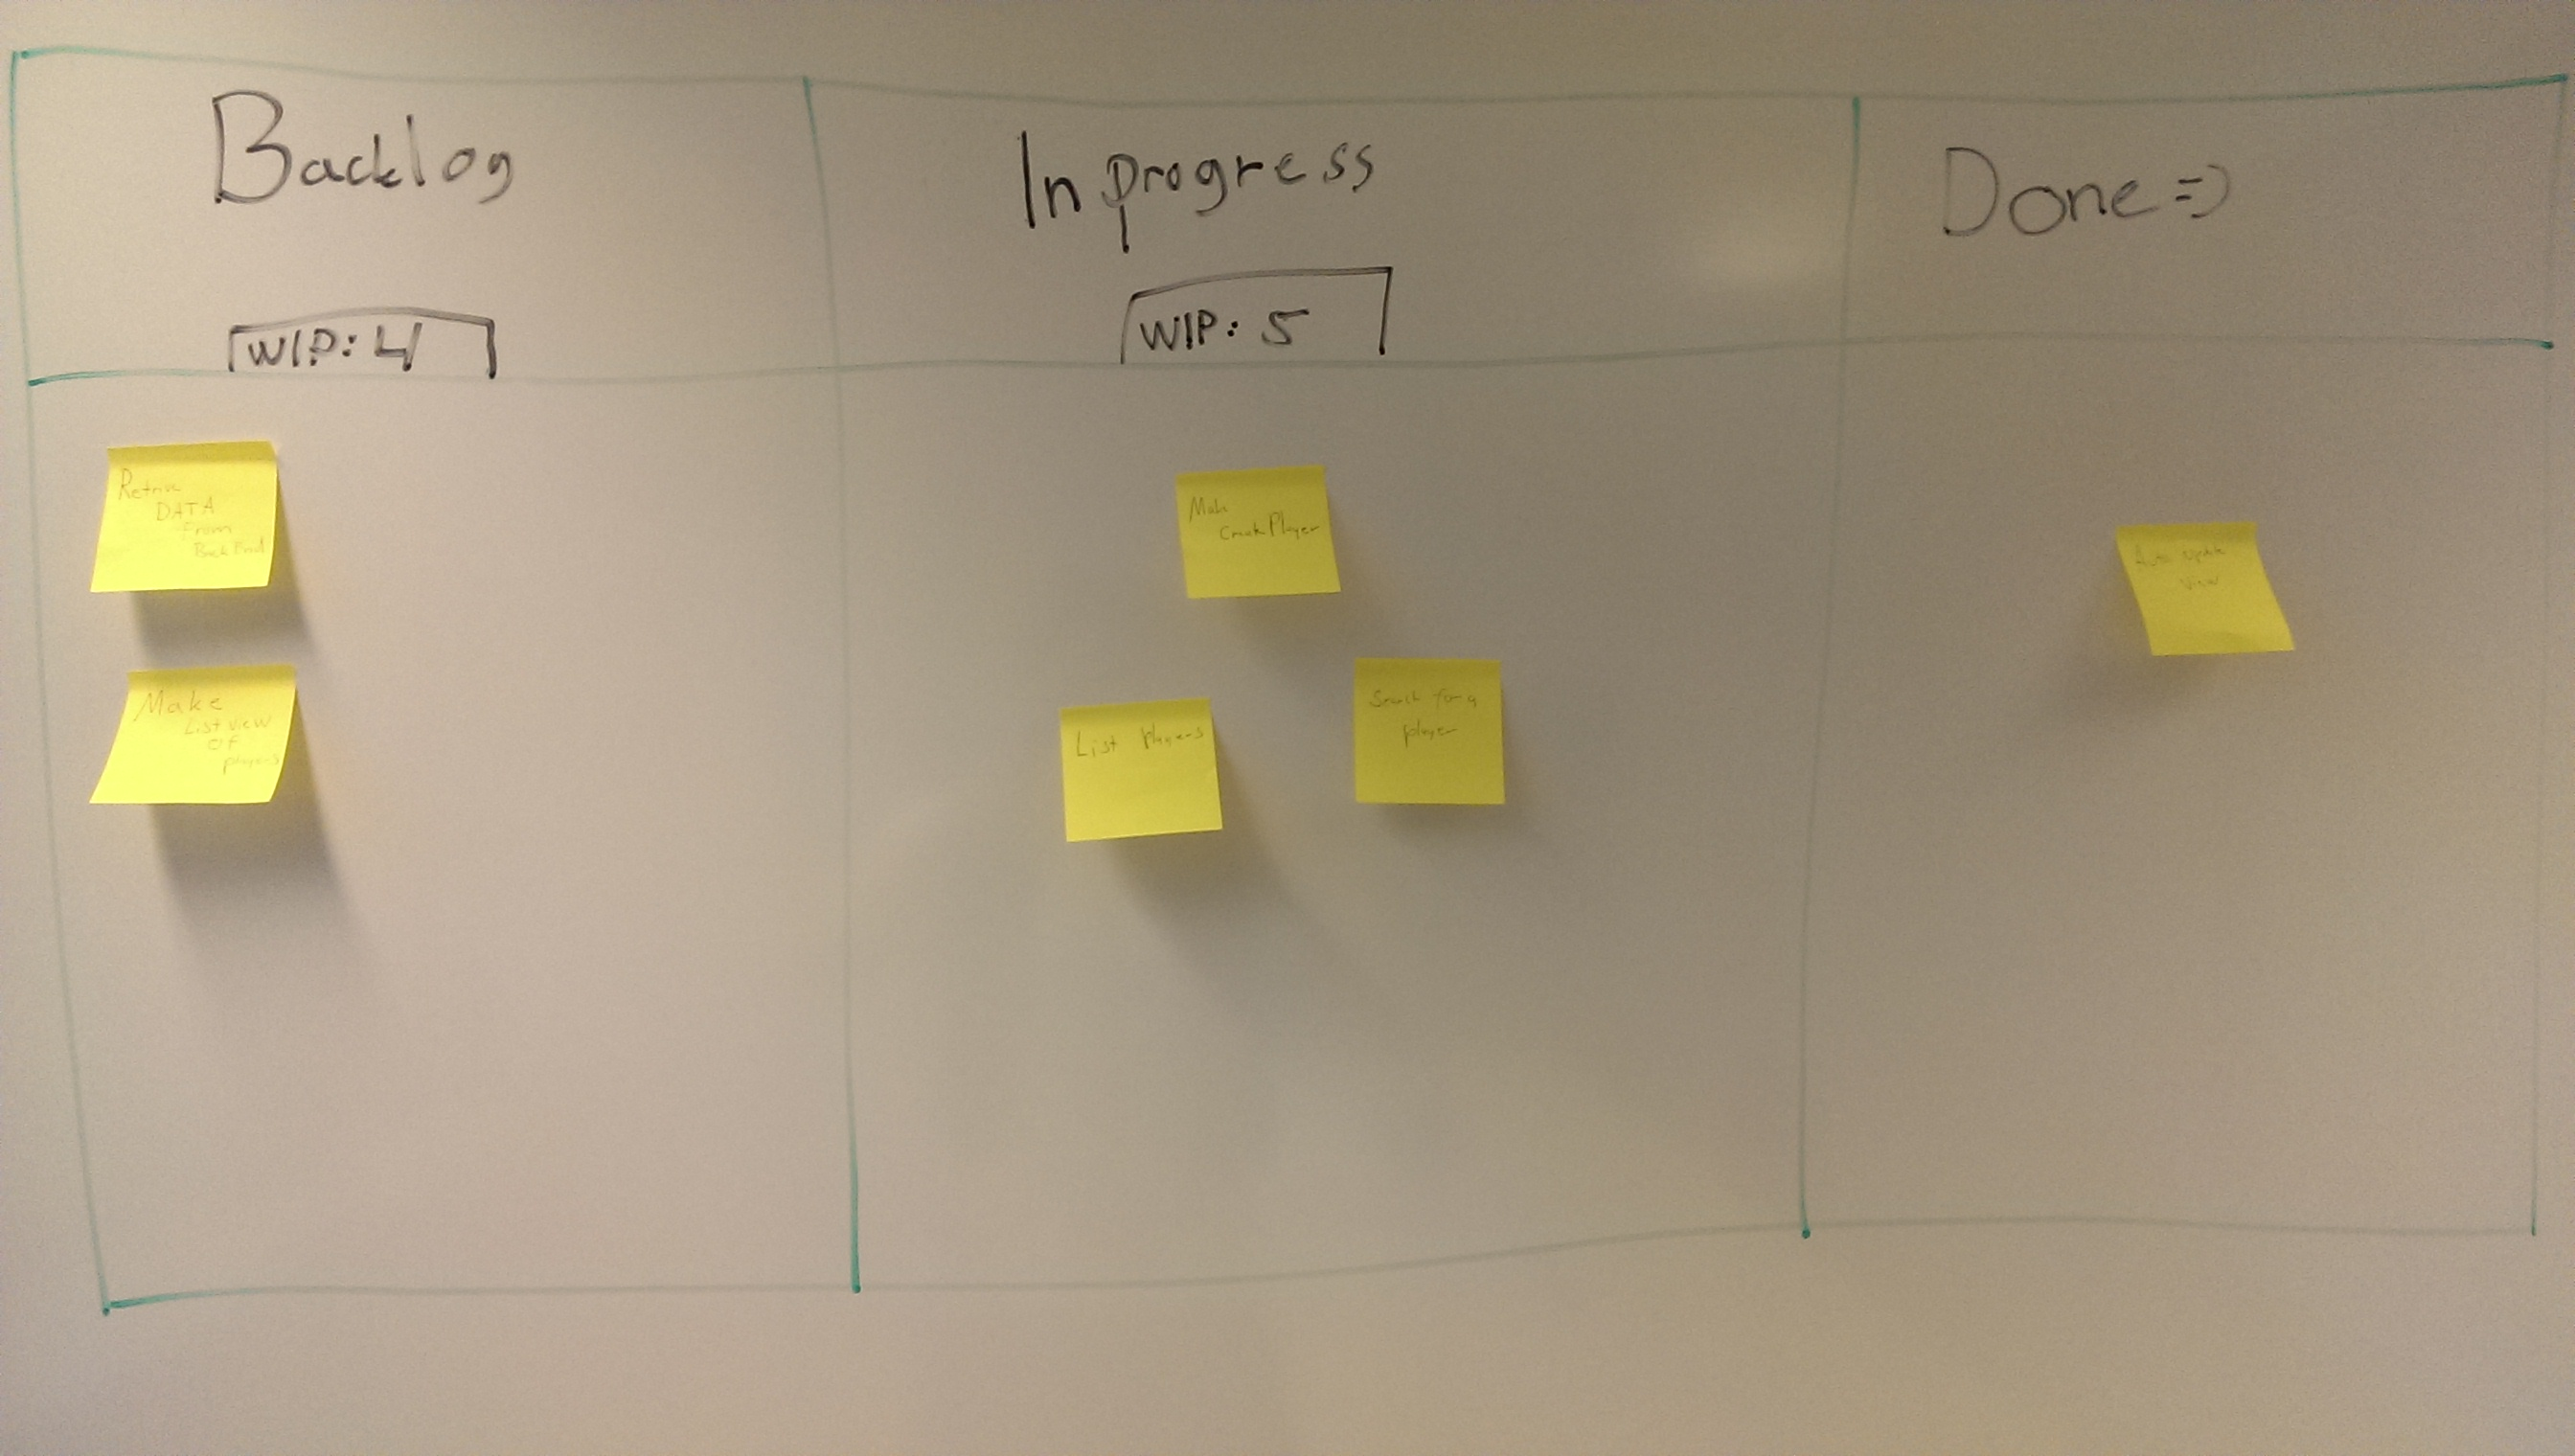
\includegraphics[width=\textwidth]{Picture/kanban_board.jpg}
\caption{Example of a Kanban board}
\label{kanban_board}
\end{figure}

\subsection{WIP limit}
\label{WIPsec}
''WIP limits seem to be the worst understood part of the Kanban system. When used properly, it exposes bottlenecks and reduces lead time for individual work items. Used improperly, it can starve developers for work or result in too many people working on the same work items.'' \parencite{Shinkle}

WIP limit is one of the core principles in Kanban \parencite{6068363}. WIP limit helps to reduce overhead by limit task-switching for each developer and make constant flow of tasks throughout the development \parencite{DavidAnderson}. One way to explain WIP and the assertion impact of WIP limit is to use cars and roads as analogy. All roads have a maximum capacity of cars. When this limit is reached, traffic jam occurs and the throughput of cars decreases and lead time increases. The same can be said about software development teams. A software team has a maximum number of tasks they can perform, if the team is pushed over the maximum limit, the throughput of tasks may decreases and lead time may increases.

When first implementing Kanban, Shinkle explains that the users don't care about WIP or setting a WIP limit, but rather the visibility of Kanban through the Kanban board. When users gain more experience with Kanban, they start to attempt the principles of WIP limit \parencite{Shinkle}. Srinivasan, Ebbing and Swearing said that setting the WIP limit is not easy. They suggest that the WIP limit is set, and then observe throughput, and adjust after that \parencite{Mandyam}. In the book "Kanban and Scrum - making the most of both" suggests Kniberg that you start by limiting WIP, then experiment with it \parencite{Kniberg}. The article "Lean Software Management" \parencite{Kniberg} and the "Impact of Kanban on Software Project Work" \parencite{Ikonen} both suggest that WIP should be minimized as well. The conclusion of present study is to keep the WIP limit low and experiment by slowly increase the WIP limit until the throughput decreased and lead time increased, then you know that the previous WIP limit was the perfect one.

The importance of limit WIP has been stated by various researches. A summary of benefits with WIP limit is stated in Section \ref{sub:sub:benefits} .  The articles by Giulio Concas, Hongyu Zhang \parencite{SMR:SMR1599}  and David Anderson, Giulio Concas, Maria Ilaria Lunesu, and Michele Marchesi \parencite{DavidAnderson} researched the difference between limit WIP and unlimited WIP.  A summary of this two articles are stated in Section \ref{sub:wip:vs:wip}

On how to determine WIP limit one article was found. If one implements Kanban with sprints or uses Scrum, \L ukasz proposes to use the effectiveness metric to help determine the WIP limit.The effectiveness metric shown in formula \ref{WIPEQ}, should be applied after end sprint according to \L ukasz. After each sprint, one can apply the effectiveness metric and the result could be used as a guideline for WIP limit for the next sprint. The effectiveness metric takes the number of bugs found \textit{(ai)} and the number of bugs found by external people (e.g. lawyers, accountants, coaches, consultants, translators, internal and external service providers etc.) \textit{(ei)}, and minus \textit{ai} and \textit{ei}, then divide the result by \textit{ai} and multiply it by 100\%  as shown in formula \ref{WIPEQ} \parencite{Sienkiewicz}

\begin{equation} \label{WIPEQ}
Ei=\frac{(ai-ei)}{ai}*100\%
\end{equation}

\subsection {Limit WIP vs. Unlimited WIP}
\label{sub:wip:vs:wip}
In the article by Giulio Concas and Hongyu Zhang, they compared the ability between WIP-limit and unlimited WIP by simulation a software maintenance process.The paper simulated two different software maintenance processes. The first process where based on 4 years of experience with Microsoft maintenance team. The second process where from a Chinese software firm.  The simulation executed 10 runs and one of the results showed that the average of closed tasks was 4145 when the WIP was limited and 3853 when the limit was not limited (about 7\% less). The paper concludes their finds; developers are more focused on fixing few issues, because the number of issues they can work on is limited. The developers are more likely to continue on the issue from the day before, rather than starting on another issue, this reduces overhead. Because when developers start on a new issue, they need time to familiarize themselves with the code and the issue. That could create unnecessary overhead if some developer already has done it, but that developer is now working on another issue. The study also showed that limit WIP can improve throughput and work efficiency \parencite{SMR:SMR1599}.

The case by David Anderson et al. \parencite{DavidAnderson} did a simulation of the impact of WIP limit vs. no WIP limit on developers with skills in different activities. The four skill activities from the article where design, development, testing and deployment. 

The article did four different simulations.  A simulation with WIP limits and seven developers with skill in two of the four activities. A simulation with no WIP limit and seven developers with skilled in two of the four activities. A simulation with WIP limits and seven developers with skill in all of the activities. A simulation with no WIP limits and seven developers with skill in two of the four activities.

The paper concluded that the last two is unlikely in the real world, since there is seldom a whole team with developers skilled in all activities. 
When the developers had skill in two out of four activities, the WIP limit simulation used 100 days, but the non WIP limit simulation used 120 days. The simulation with WIP limit shown an almost constant flow of features that completed, while in the same simulation with no WIP limit, the flow of feature was much more irregular\parencite{DavidAnderson}.

\subsection{Benefits with setting WIP limit}
\label{sub:sub:benefits}
This subsection contains excerpt from papers from various authors that have done study on WIP limit. 

\begin{enumerate}
\item Lowering the WIP limit will help people avoid task switching. When one is task switching it's hard to be able to fully concentrate. \parencite{Ikonen}.
\item There's stated when using short-cycle times and Kanban board to limit WIP, the software development team's learning is increased \parencite{Joyce}:
\item WIP increases productivity \parencite{Joyce}.
\item Limit WIP helps team to reduce overhead \parencite {CONWIP}.
\item Limit WIP decrease lead time \parencite {CONWIP}.
\item Limit WIP increase throughput \parencite {CONWIP}.
\item Limit WIP reduces flow times \parencite {CONWIP}.
\item Limit WIP reduces variation \parencite {CONWIP}.
\item Limit WIP improves quality \parencite {CONWIP}.
\end{enumerate}

Both the studies on WIP limit vs. No limit, the articles and research shows the importance of WIP limit. If  \L ukasz's effectiveness metric is isregarded , there is no clear rule on how to determine WIP limit even though WIP is suppose to be a crucial principle in order to take full advantages of Kanban.

\section {Lead time}
''Lead time is the total elapsed time from when a customer requests software to when the finished software is released to the customer'' \parencite{Joyce}.

Lead time is an essential ingredient when you look for the optimal WIP, if there is one. Often in a project, lead time is split into pieces, so every task has its own lead time. This gives the development teams the advantages to experiment with different WIPs in order to see the different lead times and then measure which WIP that suits this project the best. 

According to the paper "Quantifying the effect of Using Kanban versus Scrum" \parencite{Dag} the citation by Middleton and Joyce above is close to definition of what lead time is. They define lead time as the amount of time that passed from the moment that the development team receives a request to the moment that it completes the work item. The reason why the paper disapproves the definition by Middleton and Joyce is because: "The amount of time a work item remains in the backlog queue before it's put on the board is a function of priority, not whether the company uses Scrum, Kanban or other development methods. Furthermore, companies that develop and sell products to many customers might propose new features themselves and put them on the backlog before any customers request them. Second, given a policy of two or three releases a year, the result of a work item isn't delivered to the customer immediately after it's finished'' \parencite{Dag}.



\section{Just-In-Time}
"Just-In-Time is based on delivering only the necessary products, to the necessary time and the necessary quantity" \parencite{JIT}.

Just-In-Time (JIT) was introduced in the 1970s by Toyota in combination with Lean \parencite{javadian2013just}.  JIT has been introduced to increase productivity through waste reduction and increasing the value added in the production processes. To explain the JIT principle, Mary and Tom Poppendieck use the picture shown in Figure \ref{JITE}  \parencite{JIT} \parencite{Lean:2006}. The stream reflects the inventory.  Under the stream, there are rocks located in different sizes. The rocks illustrates waste and problems that can occur.  If the stream level is lowered, the rocks are more visualized. At this point you have to clear out rocks (remove waste and problems) in order to make the boat continue it's journey, or it will crash into the rocks. After the rocks are cleaned out, one can lower the stream level again and continue until there are pebbles left. Then the boat can float without problems.

If one lower the stream (inventory), problems and waste will become visible (visualized by rocks). Lean wants to lower inventory in order to make problems and waste occur, because when problems and waste occurs, you are able to fix the problems and remove the waste. Fixing the problem and removing the waste has several benefits such as, your process could be optimized and you are on step closer to have zero problems and zero waste.  \parencite{JIT} \parencite{Lean:2006}.

In Software development the JIT principle means that one should not deliver anything before its demand. For example, if a development team adds two new features to a product without the stakeholders asking for it and use a work day on these features, and the stakeholders don't want the features. Then the development team has produced the number of team members persons days of waste. 

\begin{figure}[ht!]
\centering
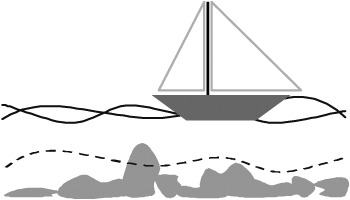
\includegraphics[width=90mm]{Picture/JIT.jpg}
\caption{JIT example}
\label{JITE} % JIT example
\end{figure}

\section{Throughput}
''The output of a production process (machine, workstation, line plant) per unit time (e.g., parts per hour) is defined as the systems throughput or sometimes throughput rate'' \parencite{Adams}.

The main concept of throughput is to measure how productive teams, people or companies are. Throughput is measured in number of finished delivered tasks or units per hour, day, week, month, quarter or year. A key factor in successfully measuring throughput in software development is to specify a standard size for each task. If the standard is not specified there is little use in throughput measurements.  \parencite{Throughput}. To illustrate throughput with different task sizes. 

Lets say Team x had a throughput of eighteen tasks after the first quarter, twenty after the second, fifteen after the third and twelve after the last quarter. Team x used Scrum the first two quarters and Kanban the last two as illustrated in table \ref{tt}. It will look like team x benefits most from Scrum. But if the task during the Kanban time was twice the size of Scrum, Kanban would suite team x the best. So, to get valid result from throughput measurements, the size of tasks has to be agreed upon by the teams or company.
\begin{table}[ht]
\begin{center}
    \begin{tabular}{| l | l | l | l |}
    \hline
    Quarter & Throughput & Method\\ \hline
    1 & 18 & Scrum\\ \hline
    2 & 20 & Scrum \\ \hline
    3 & 15 & Kanban\\ \hline
    4 & 12 & Kanban\\ \hline
    \end{tabular}
\caption{Throughput}
\label{tt} %% throughput table
\end{center}
\end{table}

\section{Code churn}
\label{sec:Churn}
"Churn is defined as the sum of the number of lines added, deleted, and modified in the source code" \parencite{Dag}.

Churn is a measure that's not so known as lead time, throughput or WIP. Churn is a term that's used as surrogates for effort in software engineering. Many studies in software engineering use code churn or revisions as surrogate measure of effort \parencite{yamashita2012quantifying}. Emam stated that "analysts should be discouraged from using surrogate measures, such as code churn, unless there is evidence that they are indeed good surrogates \parencite{el2000methodology}."  But, the study by Sjøberg et al. showed that churn could be used as a surrogate for task sizes \parencite{yamashita2012quantifying}. 


\section{Software Innovation}
\label{sec:SI}
Software Innovation is a Scandinavian software company. SI develops and delivers Enterprise Content Management applications that helps organizations improve and increase efficiency in document management, case handling and technical document control. SI builds products around the Microsoft Sharepoint platform. \parencite{Dag}. \parencite{SI}.

SI has approximately 300 employees in Oslo, Copenhagen, Stockholm and Bangalore \parencite{SI}. From 2001 to 2006, SI used the Waterfall process. In 2007, SI changed to Scrum, and in 2010, SI went from Scrum to Kanban \parencite{Dag}.

\subsection{Teams}
Table \ref{table:teams} shows the size of the ten teams vs. quarter. Team four shown in table \ref{Team:4} is the it-support team for SI. 
%DEL EN TEAM 1-4
\begin{table}[!htbp]
  \begin{adjustwidth}{-0cm}{}
\subfigure[Team one]{
 \label{Team:1}
 \scalebox{0.50}{
\begin{tabular}{ | l | r | r | }
\hline
 \bf{Year} & \bf{Quarter} & \bf{Team Size} \\ \hline
2010 & 3 & 6 \\ \hline
	2010 & 4 & 3 \\ \hline
	2011 & 1 & 16 \\ \hline
	2011 & 2 & 28 \\ \hline
	2011 & 3 & 2 \\ \hline
	2011 & 4 & 38 \\ \hline
	2012 & 1 & 35 \\ \hline
	2012 & 2 & 34 \\ \hline
	2012 & 3 & 32 \\ \hline
	2012 & 4 & 29 \\ \hline
	2013 & 1 & 24 \\ \hline
	2013 & 2 & 37 \\ \hline
	2013 & 3 & 23 \\ \hline
	2013 & 4 & 23 \\ \hline
	Total & & 330  \\ \hline
\end{tabular}
}
}
\subfigure[Team two]{
 \label{Team:2}
 \scalebox{0.50}{
\begin{tabular}{ | l | r | r | }
\hline
 \bf{Year} & \bf{Quarter} & \bf{Team Size} \\ \hline
	2010 & 3 & 10 \\ \hline
	2010 & 4 & 15 \\ \hline
	2011 & 1 & 13 \\ \hline
	2011 & 2 & 12 \\ \hline
	2011 & 3 & 15 \\ \hline
	2011 & 4 & 14 \\ \hline
	2012 & 1 & 15 \\ \hline
	2012 & 2 & 7 \\ \hline
	2012 & 3 & 8 \\ \hline
	2012 & 4 & 9 \\ \hline
	2013 & 1 & 10 \\ \hline
	2013 & 2 & 7 \\ \hline
	2013 & 3 & 7 \\ \hline
	2013 & 4 & 8 \\ \hline
	Total & & 150  \\ \hline
\end{tabular}
}
}
\subfigure[Team three]{
 \label{Team:3}
 \scalebox{0.50}{
\begin{tabular}{ | l | r | r | }
\hline
 \bf{Year} & \bf{Quarter} & \bf{Team Size} \\ \hline
2010 & 3 & 6 \\ \hline
	2010 & 4 & 9 \\ \hline
	2011 & 1 & 7 \\ \hline
	2011 & 2 & 10 \\ \hline
	2011 & 3 & 9 \\ \hline
	2011 & 4 & 10 \\ \hline
	2012 & 1 & 11 \\ \hline
	2012 & 2 & 11 \\ \hline
	2012 & 3 & 13 \\ \hline
	2012 & 4 & 13 \\ \hline
	2013 & 1 & 13 \\ \hline
	2013 & 2 & 7 \\ \hline
	2013 & 3 & 8 \\ \hline
	2013 & 4 & 8 \\ \hline
	Total & &135  \\ \hline
\end{tabular}


}
}
\subfigure[Team four]{
 \label{Team:4}
 \scalebox{0.50}{
\begin{tabular}{ | l | r | r | }
\hline
 \bf{Year} & \bf{Quarter} & \bf{Team Size} \\ \hline
	2010 & 3 & 3 \\ \hline
	2010 & 4 & 8 \\ \hline
	2011 & 1 & 4 \\ \hline
	2011 & 2 & 4 \\ \hline
	2011 & 3 & 4 \\ \hline
	2011 & 4 & 4 \\ \hline
	2012 & 1 & 4 \\ \hline
	2012 & 2 & 2 \\ \hline
	2012 & 3 & 3 \\ \hline
	2012 & 4 & 5 \\ \hline
	2013 & 1 & 7 \\ \hline
	2013 & 2 & 5 \\ \hline
	2013 & 3 & 5 \\ \hline
	2013 & 4 & 5 \\ \hline
	Total & &63  \\ \hline
\end{tabular}
}
}
\end{adjustwidth}

%%%%%%% DEL TO TEAM 5-8
  \begin{adjustwidth}{-0cm}{}
\subfigure[Team five]{
 \label{Team:5}
 \scalebox{0.50}{
\begin{tabular}{ | l | r | r | }
\hline
 \bf{Year} & \bf{Quarter} & \bf{Team Size} \\ \hline
	2010 & 3 & 5  \\ \hline
	2010 & 4 & 13  \\ \hline
	2011 & 1 & 14  \\ \hline
	2011 & 2 & 25  \\ \hline
	2011 & 3 & 21   \\ \hline
	2011 & 4 & 23   \\ \hline
	2012 & 1 & 25   \\ \hline
	2012 & 2 & 19   \\ \hline
	2012 & 3 & 24   \\ \hline
	2012 & 4 & 18   \\ \hline
	2013 & 1 & 31   \\ \hline
	2013 & 2 & 29   \\ \hline
	2013 & 3 & 27   \\ \hline
	2013 & 4 & 11   \\ \hline
	Total & &285  \\ \hline
\end{tabular}
}
}
\subfigure[Team six]{
 \label{Team:6}
 \scalebox{0.50}{
\begin{tabular}{ | l | r | r | }
\hline
 \bf{Year} & \bf{Quarter} & \bf{Team Size} \\ \hline
	2010 & 3 & 5  \\ \hline
	2010 & 4 & 6  \\ \hline
	2011 & 1 & 6  \\ \hline
	2011 & 2 & 6  \\ \hline
	2011 & 3 & 5   \\ \hline
	2011 & 4 & 5   \\ \hline
	2012 & 1 & 4   \\ \hline
	2012 & 2 & 6   \\ \hline
	2012 & 3 & 6   \\ \hline
	2012 & 4 & 9   \\ \hline
	2013 & 1 & 9   \\ \hline
	2013 & 2 & 9   \\ \hline
	2013 & 3 & 9   \\ \hline
	2013 & 4 & 14   \\ \hline
Total & &99  \\ \hline
\end{tabular}
}
}
\subfigure[Team Seven]{
 \label{Team:7}
 \scalebox{0.50}{
\begin{tabular}{ | l | r | r | }
\hline
 \bf{Year} & \bf{Quarter} & \bf{Team Size} \\ \hline
 	2010 & 3 & 10  \\ \hline
	2010 & 4 & 8   \\ \hline
	2011 & 1 & 8   \\ \hline
	2011 & 2 & 6   \\ \hline
	2011 & 3 & 8   \\ \hline
	2011 & 4 & 9   \\ \hline
	2012 & 1 & 10   \\ \hline
	2012 & 2 & 5   \\ \hline
	2012 & 3 & 9   \\ \hline
	2012 & 4 & 3   \\ \hline
	Total & &76  \\ \hline
\end{tabular}
}
}
\subfigure[Team eigth]{
 \label{Team:8}
 \scalebox{0.50}{
\begin{tabular}{ | l | r | r | }
\hline
 \bf{Year} & \bf{Quarter} & \bf{Team Size} \\ \hline
 	2010 & 4 & 2 \\ \hline
	2011 & 1 & 8 \\ \hline
	2011 & 2 & 8 \\ \hline
	2011 & 3 & 13 \\ \hline
	2011 & 4 & 9 \\ \hline
	2012 & 1 & 10 \\ \hline
	2012 & 2 & 2 \\ \hline
	2012 & 3 & 25 \\ \hline
	2012 & 4 & 11 \\ \hline
	2013 & 1 & 22 \\ \hline
	2013 & 2 & 21 \\ \hline
	2013 & 3 & 23 \\ \hline
	2013 & 4 & 8 \\ \hline
	Total & &162  \\ \hline
\end{tabular}
}
}
\end{adjustwidth}




%%%%%% DEL tree TEAM 9-10
  \begin{adjustwidth}{2cm}{}
\subfigure[Team nine]{
 \label{Team:9}
 \scalebox{0.50}{
\begin{tabular}{ | l | r | r | }
\hline
 \bf{Year} & \bf{Quarter} & \bf{Team Size} \\ \hline
 	2010 & 4 & 5 \\ \hline
	2011 & 1 & 8 \\ \hline
	2011 & 2 & 7 \\ \hline
	2011 & 3 & 7 \\ \hline
	2011 & 4 & 9 \\ \hline
	2012 & 1 & 10 \\ \hline
	2012 & 2 & 8 \\ \hline
	2012 & 3 & 10 \\ \hline
	2012 & 4 & 12 \\ \hline
	2013 & 1 & 8 \\ \hline
	2013 & 2 & 9 \\ \hline
	2013 & 3 & 8 \\ \hline
	2013 & 4 & 8 \\ \hline
	Total & &109  \\ \hline
\end{tabular}}
}
\subfigure[Team ten]{
 \label{Team:10}
 \scalebox{0.50}{
\begin{tabular}{ | l | r | r | }
\hline
	 \bf{Year} & \bf{Quarter} & \bf{Team Size} \\ \hline
	2010 & 3 & 3 \\ \hline
	2010 & 4 & 11 \\ \hline
	 2011 & 1 & 12 \\ \hline
	 2011 & 2 & 9 \\ \hline
	2011 & 3 & 4 \\ \hline
	 2011 & 4 & 17 \\ \hline
	2012 & 1 & 20 \\ \hline
	2012 & 2 & 17 \\ \hline
	2012 & 3 & 18 \\ \hline
	2012 & 4 & 13 \\ \hline
	2013 & 1 & 17 \\ \hline
	2013 & 2 & 9 \\ \hline
	2013 & 3 & 10 \\ \hline
	2013 & 4 & 10 \\ \hline
	Total & &170  \\ \hline
\end{tabular}
}
}
\end{adjustwidth}
\caption[Optional caption for list of figures]{Caption of team size for teams in SI}
\label{table:teams}
\end{table}




\chapter{Research Methods}
\label{chap:RM}
In this chapter the research methods will be introduced and the reason why the data from Software Innovation where chosen for this master thesis will be stated. Section \ref{sec:CS} gives a brief introduction to the research method "Case Study".  Section \ref{sec:coc} is about the choice of case and complementary information about SI. 


\section{Case study}
\label{sec:CS}
To answer the research questions, a case study was conducted.  A case study is used to explore causation in order to find underlying principles \parencite{0078285763}\parencite{9781412960991}.  But which methods one can use in a case study or how the case study is conducted is ambiguous.  It might be that the case study maybe qualitative or quantitate.  A case study might utilize a particular type of evidence (for example ethnographic, participant observation or field research).  Jennifer Platt stated: "Much case study theorizing has been conceptually confused because too many different themes have been packed into the idea "case study" \parencite{0521676568}.  John Gerring stated: "A case study may be understood as the intensive study of a single case where the purpose of that study is -- at least in part to shed light on a larger class of cases  \parencite{0521676568}.As shown there is no clear rule what exactly a case study is.


%John also stated: "Case connotes a spatially delimited phenomenon (a unit) observed at a single point in time or over a period of time"\parencite{0521676568}. 
In this thesis, the case study is used to explore WIP limit's effect in software development. The purpose is to shed light on WIP limit in software development and if it matters. In order to do so, the data set from SI with quantitative data was analyzed.

\section{Choice of case}
\label{sec:coc}
The data set from SI contains information about each task SI has worked rom 2008 to 2013. The data set is represented in a excel document. An excerpt of some of the columns in the document is shown in table \ref{dataset}. Although the data set contains items from 2008-2013, data from year 2008, 2009 and the two first quarters of 2010 will be excluded. The dates will be excluded partially because the transition from between processes and it was inaccurate measurements when SI first started with TFS.

The reason SI and the data set from SI is analyzed in this thesis is because the article "Quantifying the Effect of Using Kanban versus Scrum" \parencite{Dag} used the same data set. Since Dag is the supervisor of this thesis and he had access to the data set, to use the set from SI is a choice of convenience. 

\begin{table}[!ht]
\begin{center}
\begin{tabular}{|l|l|l|l|l|l|l|}
\hline
ID	& Type &  Created Date & From Day & Date To & Lead Time & Team \\ \hline
    3027 & Bug & 2008-10-07 &  2008-10-09 & 2008-10-16 & 20 & Team one\\ \hline
   3028 & Bug  & 2008-10-07 & 2008-10-07 & 2008-10-08 & 10 & Team six\\ \hline
   3029 & Feature & 2008-10-07 &  2008-12-30	 & 2008-12-30 & 105 & Team two\\ \hline
    3030 & Feature & 2008-10-07 & 2008-10-07	& 2008-10-07 & 1& Team three\\ \hline
   3035 & Bug & 2008-10-08 & 2008-11-20 & 2008-11-28 & 17 & Team five\\ \hline
   3037 & Feature & 2008-10-08 &  2008-10-19	 & 2008-10-19 & 7 & Team three\\ \hline
   3040 & Bug & 2008-10-10 &  2008-11-19 & 2008-11-19 & 48 & Team one\\ \hline
   \end{tabular}
\caption{Excerpt from the data set}
\label{dataset}
\end{center}
\end{table}

The data set contains thirty columns with different data for each task, mostly of this columns are irrelevant for this study but the important columns is stated in table \ref{IC}.

\begin{table}[!ht]
\begin{center}
    \begin{tabular}{| l | p{5cm} |}
    \hline
     \bf{Variable} & \bf{Description}\\ \hline
     Created Date & When a task is put in backlog \\ \hline
     Date From & When a given task is pulled out from the backlog\\ \hline
     Date to & When a task is finished and ready for release. \\ \hline
    Lead Time & The amount of days elapsed from the date the task was created until the tasks has finished  \\ \hline
   Type & The type column is labeled as either bug or feature depending on the type of the task \\ \hline
   Lines added & Number of lines added to a feature or bug \\ \hline
   Lines modified & Number of lines modified when working on a feature or bug \\ \hline
   Lines deleted & Number of lines deleted from a bug or feature \\
    \hline
    Team &States the team who has been working on the task.\\ \hline
    \end{tabular}
\caption{Variables from the SI dataset}
\label{IC} %% information columns
\end{center}
\end{table}

\newpage

The data from SI was analyzed on team level. The data from SI was analyzed using the program, which will compute the variables shown in table \ref{des} for all of the teams.
\begin{table}[htbp]
\begin{center}
    \begin{tabular}{| l | p{5cm} |  p{5cm} |}
    \hline
    \bf{Computed variable} &	\bf{Description}	 & \bf{Columns from SI}\\ \hline 
     WIP & \parbox[t]{5cm}{Items in progress on the given day} & Date From and Date To. \\ \hline
     Throughput	& Number of tasks finished on a given day & Date To \\ \hline
     Churn & Lines added, lines modified and lines deleted added together & Lines Added, Lines Modified, Lines Deleted and Date To \\ \hline
    Bugs & The number of tasks labeled as Bug and not feature & Type and Created Date \\ \hline
    Lead time & The time used on a task, measured in days & Lead time and Date To \\ \hline
    Bugs finished, quarter & Number of bugs finished, per quarter &Created date, Date to and Type \\ \hline
    Avg days backlog, bug & Average days in backlog for bugs, per quarter & Created date, Date from and Type \\ \hline
  \end{tabular}
\caption{Relationship between variable and columns from SI}
\label{des} %% desription
\end{center}
\end{table}
\newpage
The \textbf{Date from} column consist of dates form when tasks where created. 
The \textbf{Date to} column consist of all of the dates when tasks where marked as finished.
The \textbf{Lines added}, \textbf{Lines Modified} and \textbf{Lines Deleted} columns contains the amount of lines added, modified or deleted in order to finished the task.
The \textbf{Type} column consist of a string that has the value as either "Bug" or "Feature".
The \textbf{Lead time} column consist of the lead time value. 
 
Both the variables churn and throughput is split up in two sub variables with suffix of "Feature" and "Bug". The variable with suffix of "Feature" means tasks labeled with type "feature" are the only one who is counted. The same goes for variables with suffix "Bug". The "Bugs finished, quarter" variable represents how many tasks labeled "Bug" that are finished within the same quarter as it was created.  The "Avg days backlog, bug" variable represent the average number of days bugs are in backlog before it pulled out. These two variables are used as an indicator of the workload together with churn.   




\subsection{Software Innovation's development process}
From 2001 to 2006 SI used the Waterfall process with a life cycle of:
\begin{enumerate}[noitemsep,topsep=0pt,parsep=0pt,partopsep=0pt]
\item Design
\item Implementation 
\item Testing
\item Deployment for each new release
\end{enumerate} 
\parencite{Dag}. 

In 2007, SI examined their development process, which resulted in a decision to change to Scrum. Scrum was implemented with the standard elements of Scrum:
\begin{itemize}[noitemsep,topsep=0pt,parsep=0pt,partopsep=0pt]
\item Cross functional teams
\item Sprint planning meetings 
\item Estimation of work items using planning poker
\item Daily standup meetings
\item Sprints
\end{itemize}
\parencite{Dag}. 

SI implemented three weeks sprint, after each sprint a fully tested shippable code was ready. In 2010, SI went from Scrum to Kanban. SI felt that Scrum was too rigid and didn't fit their purpose, they also feared that inaccurate estimation and time boxing gave them longer lead time. SI also saw Scrum planning meetings as waste which reduced productivity and quality \parencite{Dag}. 

SI decided to implement Kanban in the following manner. When a work item is pulled from the backlog, SI tries to make the item flow through all the stages until it's ready for release. This procedure happens as quickly as possible. In order for an item to be ready for release, it has to be at a satisfactory quality level, which is defined by SI. SI also implemented WIP limits. If the WIP limit is reached, no new tasks are started until another task is finished which is based on the principle of just-in-time \parencite{Dag}.


\chapter{Data collected and calculations}
\label{ch:DCC}
This chapter will introduce how the algorithms of the program works. The first section, Section \ref{WPD} introduces the algorithm of how the program measure WIP for each day. The subsection \ref{sec:Example} provides a comprehensive example of how the program measure WIP per day. The consecutively sections reveal the algorithm of how the program measure bugs (Section \ref{sec:bug}) throughput (Section \ref{sec:TP}),  churn (Section \ref{sec:churn}) and lead time (Section \ref{sec:LT}). In the last section, a short introduction to the statistical analyze program SPSS is given (Section \ref{sec:SPSS}). For this thesis a program was made in order to measure the variables shown in Table \ref{des}. %The explanation of how the program works will be split into sections so it will be easier to get a understanding of how the program operates. The explanation of how the program works will first contain a detailed description in words, then a description using Pseudocode \parencite{jd}.The Pseudocode for each section is simplified with only the key elements of the program code. 


The Table \ref{tab:measurementDone} shows how quarters, dates and days are represented in this thesis. 

\begin{table}[!ht]
\centering
\begin{itemize}
\item The Date standard is specified as YYYY-MM-DD.
\item All seven days in the week are taken into account when measuring included Saturdays and Sundays
\item Quarter of a year is defined as: 
\begin{itemize}
\item January, February and March (Q1),
\item April, May and June (Q2),
\item July, August and September (Q3),
\item October. November and December (Q4).
\end{itemize}
\parencite{Quarter}
\caption{The standard of the data set}
\label{tab:measurementDone}
\end{itemize}
\end{table}



\section{SPSS}
\label{sec:SPSS}
"IBM\circledR  SPSS\circledR Statistics is a comprehensive system for analyzing data. SPSS Statistics can take data from almost any type of file and use them to generate tabulated reports, charts and plots of distributions and trends, descriptive statistics, and complex statistical analyses." \parencite{IBM}

After the program has finished the measurements of the data, SPSS will be used to analyze the derived data. SPSS will help to answer the research question stated in chapter \ref{chap:RQ} with help of two statistics method: correlation and case summaries. 


%%legge inn en section her go ha de andre under her som subsection?
\section {WIP per day}
\label{WPD}

%% Table \ref {dataset} show an excerpt from the SI dataset.  The date 2008-10-09 is not in the set so the the program has to create 2008-10-09 and add it to the set in order to calculate WIP, throughput, bugs and lead time per day.  Skrive her at program lager hver dato for set self

\subsection{Step 1: Gather all unique dates into a Arraylist}
\label{sub:stepOne}
The first step of WIP this programs algorithm is to create a WIP object with the attributes in table \ref{tab:object}.  The values that are assigned to the attributes are gathered from the data set file.  The program creates a WIP object and assigned the data set values to the object a shown in listing \ref{lst:Arraylist} . After the values are assigned, the program puts the WIP object into the right Arraylist\footnote{Arraylist is a resizable array implementation of a list. The Arraylist class provides function for manipulate the size of the array, check the size of the list and convert the list to an array  \parencite{Arraylist}.} based on the team variable as shown in listing \ref{lst:addWIP}. In listing \ref{lst:addWIP}.
\begin{table}[!ht]
\begin{center}
\begin{tabular}{| l | l |}
\hline
\bf{Type} & \bf{Variable name} \\ \hline
Date & start \\ \hline
Date & end\\ \hline
String & team\\ \hline
String & processType\\ \hline
int  & WIP\\ \hline
\end{tabular}
\caption{Variables of the WIP objects}
\label{tab:object}
\end{center}
\end{table}


\begin{minipage}{\textwidth} 
 \begin{lstlisting}[caption={Gather all unique dates into Arraylist},label={lst:Arraylist}]
While inputFile != EOF // EOF = End Of file
		WIP = New WIP()
		WIP.start = inputFile.start
		WIP.end = inputFile.end
		WIP.team = inputFile.team
		WIP.processType = inputFile.processType
		WIP.WIP = 1
		FindTeam(WIP)
 \end{lstlisting}
 \end{minipage}

 
 \begin{lstlisting}[caption={Gather WIP object to the right data structure},label={lst:addWIP}]
void FindTeam (WIP w) 
		if w.team EQUALS "TeamOne"
			TeamOne.add(w)
		if w.team EQUALS "TeamTwo"
			TeamTwo.add(w)
		if w.team EQUALS "TeamThree"
			TeamThree.add(w)			
/* And so on for the rest if the seven teams */
 \end{lstlisting}
 
 \newpage
\subsection{Step 2: Gather the remaining dates}
 \label{sub:stepTwo}
There are some dates missing as shown in Table \ref{wt:2} shows. For example, the date 2010-10-08 is missing. In order to generate WIP for each day, the program has to create the dates that are not in the set. In order to create the remaining dates, the program takes the first date and the last date from each of the teams's Arraylist created in previous section (\ref{sub:stepOne}) as shown in line one and two of Listing \ref{lst:remaining}. Then the program checks if all the dates between the first date and the last date are in the team's Arraylist. Each of the Arraylists are sorted on date. If the dates are not in the Arraylist, the program will put the date into the Arraylist as show in method addToArraylist on line ten to thirteen.
In order to keep the pseudocode simple, the generateWIP method stated in line twelve was omitted. The generateWIP method creates a new WIP object and returns it.



\begin{lstlisting}[caption={Gather the remaining dates.},label={lst:remaining}]
WIP first = Arraylist.get(0)//points to the first WIP object in the Arraylist 
WIP last = Arraylist.get(Arraylist.size()-1)//points to the last WIP object in the Arraylist 
Next_date //points to the next date
Next_date = first.getDate() // Next_date assigned before iteration
while Next_date NOT EQUALS last.getDate()
	New_date = Next_Date + 1 //Compute the next date
	AddToArraylist(New_date, first.getTeam())
	Next_date = New_date

void addToArraylist(Date d, String team)
	if d NOT CONTAINS IN Arraylist
		WIP = generateWIP(d, team)
		Arraylist.add(WIP) 
 \end{lstlisting}

\subsection{Step 3 Measure WIP}
\vspace{-2.0em}
The Arraylist from section \ref{sub:stepOne}  and \ref{sub:stepTwo} now contains a WIP object for each date from the third quarter of 2010 to 2013 for each team. In this step, the program will loop through each of the teams Arraylists. During the iteration each WIP object is extracted from the Arraylist and the WIP is measured. The two methods stated in line ten and eighteen respectively gather the current WIP (method in line ten) and finds out how many finished tasks (method in line eighteen) and returns the result. The result is used in six five to compute the current WIP. The if test in line four assures that there is only measured one WIP for each start date.  
\begin{minipage}{\textwidth} 
\begin{lstlisting}[caption={WIP measurement},label={lst:measure}]
void measureWIP()
	lastWIP =  0
	for WIP Object IN Arraylist	
		if(DateNotMeasured(WIP.getStartDate()) == true)
			WIP_for_this_date = get_current_WIP(WIP.getStartDate())  
			WIP_measured = WIP_for_this_date - Nr_of_finishedDates(WIP.getStartDate) + lastWIP
			WIP.setWIP(WIP_measured)
			lastWIP = WIP_measured 

int get_current_WIP(Date date)
	current_WIP = 0
	for WIP in  Arraylist
		if date EQUALS WIP.getStartDate()
			Nr_of_dates_to_decrement++
return current_WIP
			 	
int Nr_of_finished_dates(Date date)
	Nr_of_dates_to_decrement = 0
	for WIP in Arraylist
		if date AFTER WIP.getEndDate() DO
			if date not picked
				Nr_of_dates_to_decrement++
				dateIsPicked(WIP)				
return Nr_of_dates_to_decrement 
 \end{lstlisting}
  \end{minipage}

\subsection{Example}
\label{sec:Example}
This section will provide a comprehensive example of how the WIP algorithm works.  
Figure \ref{wip_timeline}  shows tasks id's in the y-axis and dates in the x-axis. The green line indicates the duration of the task. The figure helps  visualizes how many WIPs there are for a given date. For example on the date 2008-10-12, tasks 3, 5 and 6 are in progress, which means the WIP is 3 for 2008-10-12.  

In this example dates from table \ref{wt:2}  will be used to illustrate how the algorithm measure WIP.  The figure \ref{wip_timeline} visualize WIP for each date.
%skrive om tabellen
\begin{figure}[ht!]
\centering
\hspace*{-1in}
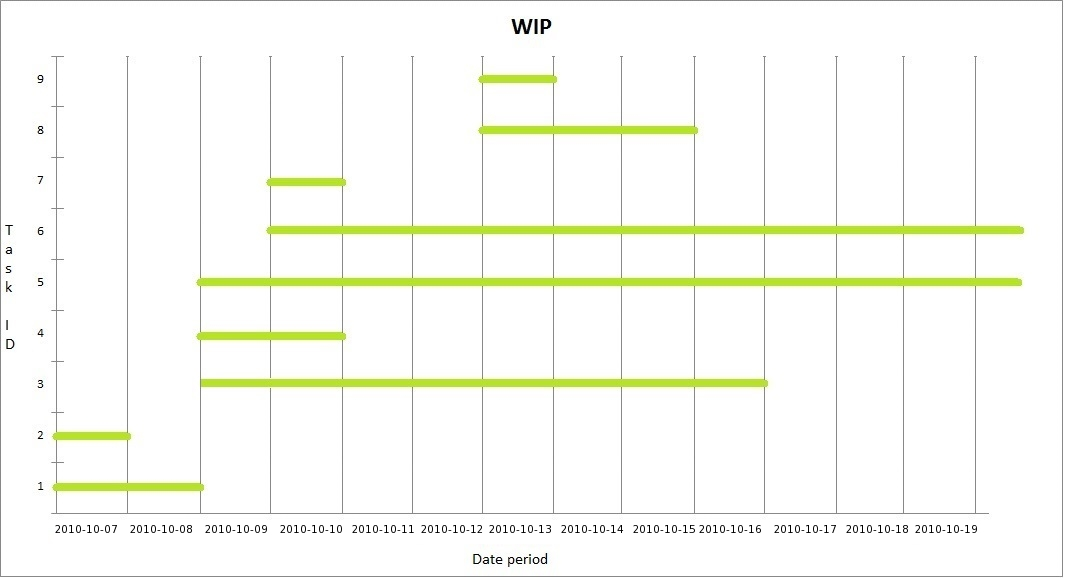
\includegraphics[width=21cm,trim=4 8 8 4,clip]{Picture/wip_example.jpg}
\caption{Illustrating the WIP timeline for example stated in section \ref{sec:Example}}
\label{wip_timeline}
\end{figure}

\newpage
\begin{table}[!ht]
\begin{center}
    \begin{tabular}{| l | l | p{2cm} | l | l |}
    \hline
   Task ID &   Date From  & Date To & Team & Process Type\\ \hline
     1 & 2010-10-07 & 2010-10-08 & Team One & Kanban  \\ \hline
     2 & 2010-10-07 & 2010-10-07 & Team One & Kanban   \\ \hline
     3 & 2010-10-09 & 2010-10-16 & Team One & Kanban   \\ \hline
     4 & 2010-10-09 & 2010-10-10 & Team One & Kanban   \\ \hline
     5 & 2010-10-09 & 2010-11-04 & Team One & Kanban   \\ \hline
     6 & 2010-10-10 & 2010-11-05 & Team One & Kanban  \\ \hline
     7 & 2010-10-10 & 2010-10-10 & Team One & Kanban   \\ \hline
     8 & 2010-10-13 & 2010-10-15 & Team One & Kanban  \\ \hline
     9 & 2010-10-13 & 2010-10-13  & Team One  & Kanban   \\ \hline
    \end{tabular}
\caption{Showing Task ID, Date From and Date to}
\label{wt:2} %%  wip table 2\
\end{center}
\end{table}

\subsubsection{Step 1}
The program will first read in the first line of table \ref{wt:2}.  The first line is the one labeled with task id one.  The program creates the WIP-object for line one and it will look like the listing \ref{lst:WIPOBJ}.  The program will follow the exact same procedure until all the dates are read in. 

\begin{minipage}{\textwidth} 
\begin{lstlisting}[caption={Creating WIP-object},label={lst:WIPOBJ}]
WIP = new WIP()
WIP.start = 2010-10-07
WIP.end = 2010-10-08
WIP.team = "Team One"
WIP.processType = "Kanban"
WIP.WIP = 1
\end{lstlisting}
  \end{minipage}

 \subsubsection{Step 2}
\label{sub:sub:st}
Now that the whole set has been read in and saved. The next thing to do is to create the remaining dates. The Arraylist contains all the dates from table \ref{wt:2}.  The program will now extract the first and the last date from the Arraylist. Before this step, the objects in the Arraylist are sorted by date. The first date is 2010-10-07 and the last date is 2010-10-13.  The program will check if the date after 2010-10-07 contains in the set, which it don't. The program then generates a WIP object for the date 2010-10-08 and adds it to the Arraylist as shown in listing \ref{lst:WIPCREATE}. After the date is created, the program will see if the date 2008-10-09 exits and will do so for all dates until the date 2010-10-13.

\begin{minipage}{\textwidth} 
\begin{lstlisting}[caption={Creating WIP-object},label={lst:WIPCREATE}]
void createNewWIP(Date d, String team) 
	WIP.start = d
	WIP.end = d
	WIP.team = team
	WIP.processType = "Uknown"
	WIP.WIP = 0
\end{lstlisting}
  \end{minipage}


\subsubsection{Step 3}
The Arraylist now contains the dates from 2010-10-08 to 2010-10-13. The next and last step is to measure WIP for each date.  The program will now loop through the Arraylists. The first date is 2010-10-07.  The get\_current\_wip method from line nine in listing \ref{lst:measure} will be called with the date 2010-10-07 as parameter.  The method will return two, since both task one and two where started at 2010-10-07 as shown by figure \ref{wip_timeline}. The next thing to do is to find out how many tasks to decrement the current WIP with.  The method Nr\_of\_fininshed\_dates in line seventeen is called with the date 2010-10-07. As shown by the table \ref{wt:2} and figure \ref{wip_timeline} there was no task finished at the date 2010-10-07, so the method returns 0. The program then updates the WIP objects' counter to two and saves the WIP in the lastWIP object. The next date is 2010-10-08, who the program made in subsection \ref{sub:sub:st}. There is no task started at 2010-10-08, but task one is finished at the date. So the Nr\_of\_fininshed\_dates returns one and flag the current date as shown in listing \ref{lst:measure} by the line twenty-three. The result of WIP\_measure in line five is 1 ($0-1+2=1$). WIP at date 2010-10-08 is one, as shown by figure \ref{wip_timeline}. The program will continue this procedure until all the dates are measured.  The reason why the date is flagged is to be sure that each day only evaluates ones. The if statement listed in listing \ref{lst:measure} at line twenty-one assurance that.

\iffalse
\subsubsection{First step}
\label{subsubsec:ft}
The program will first do a look-up on the date 2008-10-07 referred with task ID one and two in table \ref{wt:2} and measure the current WIP counter, which is two, because its two tasks in progress on this date. After this the program will put the date and the current WIP into a Arraylist. 
Now the algorithm will see if any task was done in the last period, since task one and two is the two first tasks to be measured in this example, there's no task finished in the period and there's no current WIP from other tasks, so the current WIP at 2008-10-07 is two illustrated by figure \ref{wip_timeline}. 
\subsubsection{Second step}
The program will do a look-up on the date 2008-10-09 referred with task ID three, four and five in table \ref{wt:2}  and measure the current WIP for this date, which is three. Then, the program will put the date and the current WIP into a Arraylist.
Next, the program will see that two tasks were done in the period of 2008-10-07 to 2008-10-09. So the program will measure that three new tasks were started at 2008-10-09, two where finished and the WIP from last date measure where two, so the calculation of WIP at 2008-10-09 is 3-2+2, which gives a WIP of three on 2008-10-09 illustrated by figure \ref{wip_timeline}. 

\subsubsection{Third step}
The program will do a look-up on the date 2008-10-10 referred with task ID six and seven in table \ref{wt:2}  and measure the current WIP for this date, which is two. Next the program will put the date and the current WIP into a Arraylist.
Last the program will see that no task where done in the period 2008-10-09 to 2008-10-10 and the currently WIP is three, so this gives a new WIP of 5 illustrated by figure \ref{wip_timeline}. 

\subsubsection{Fourth step}
The program will do a look-up on the date 2008-10-13 referred with task ID eight and nine in table \ref{wt:2}  and measure the current WIP for this date, which is two. Then the program will put the date and the current WIP into a Arraylist. 
Next the program will look at the period between 2008-10-10 and 2008-10-13, and see that task four and seven was done in this period. The WIP at 2008-10-13 will be $2-2+5 = 5$ as illustrated by figure \ref{wip_timeline}. 
As illustrated by the example, WIPs are not decrement until the finished date is passed, even though the task is done on the date, it's also worked on the same date, therefore the WIP is decrement after each date is passed.
\fi



\newpage
 \section{Rest of the variables}
 \label{sec:rotv}
To compute the remaining variables, churn, lead time and throughput a new algorithm is required.  The algorithm for the three variables is almost identical. First the program read in the data set from SI. For each of the lines in the data set, the program creates an object and saves the valuable information from the data set in the object. Then each object is saved in a data structure based on team association as showed in \ref{addObj}. When all the lines has been read in, and all objects has been put in the right data structure the algorithm differs. In the following subsections the algorithm for each of the variables is presented. In subsection \ref{sec:TP} the throughput algorithm is stated, in subsection \ref{sec:churn} churn is stated, in subsection \ref{sec:LT} lead time is stated and in subsection \ref{sec:bug}  a description of how bug and feature is measured 
\begin{minipage}{\textwidth}
\begin{lstlisting}[caption=Pseudocode example of how throughput objects are added, label=addObj]
void addBug(Bug b)
	if b.team EQUALS "TeamOne"
		if dateExists(b.date, TeamOne) EQUALS false
			// if date don't exists, then add the bug
			TeamOne.add(b)
			
	if b.team EQUALS "TeamTwo"
		if dateExists(b.date, TeamTwo) EQUALS false
			// if date don't exists, then add the bug
			TeamTwo.add(b)
			
	if b.team EQUALS "TeamThree"
		if dateExists(b.date, TeamThree) EQUALS false 
			// if date don't exists, then add the bug
			TeamThree.add(b)
			
	if b.team EQUALS "TeamFour"
		if dateExists(b.date, TeamFour) EQUALS false
			// if date don't exists, then add the bug
			TeamFour.add(b)
		
void dateExists(Date d, Arraylist list)
	for Bug b in list
		if b.date EQUALS d
			b.counter++
			return true
	
return false	
 \end{lstlisting}
 \end{minipage}
 
\subsection{Throughput}
 \label{sec:TP}
When the steps described in section \ref{sec:rotv} are finished, the program takes each of the data structures and compute throughput. To compute throughput, a counter representing the throughput for each date is created. The method dateExists in listing \ref{throughputCode} does the actual computation. The method starts of with a test. If the date of the throughput object is in the data structure, the corresponding counter is incremented.  If the date is not in the data structure, the new throughput object is added to the data structure. 
\begin{minipage}{\textwidth}
\begin{lstlisting}[caption=Pseudocode example of how throughput is measured, label=throughputCode]
void dateExists(Throughput tp d, Arraylist list)
	for Throughput t in list
		if t.date EQUALS tp.date
			t.counter++
			return
			
structure.add(tp);
\end{lstlisting}
 \end{minipage}


\subsection{Churn}
\label{sec:churn}
As stated in section \ref{sec:Churn} in order to take churn into account one need to know it's good surrogates. SI has gathered churn with help of Microsoft's Team Foundation Server (TFS). The TFS system automatically records data such as churn and lead time. Based on TFS one can know that churn for SI is a good surrogate.

To measure churn the data set from SI contains three columns ("Lines added, "Lines modified" and "Lines deleted") shown in table \ref{table:churn}. These three variables are summed together, and saved in a  variable called "churn" when the data set is read in. These three columns are automatically recorded by TFS.  To complete the churn measurements the three columns are multiplied.  For task id one, the churn is 2028 ($352+307+1369 = 2028$). Some tasks has zero churn, for example task with id six, these tasks don't need code in order to be finished such tasks needs technical support to be finished. The algorithm is shown in listing \ref{churnCode}

\begin{table}[!ht]
\begin{center}
    \begin{tabular}{| l | l | l | l |}
    \hline
\bf{Task id} & \bf{Lines added} & \bf{Lines modified}  & \bf{Lines deleted} \\ \hline
1&352&307&1369\\ \hline
2&314 & 31 & 15 \\ \hline
3&314&31 & 15\\ \hline
4&62&327&153 \\ \hline
5&21&3&0 \\ \hline
6&0&0&0 \\ \hline
\end{tabular}
\caption{How churn is presented in the excel document}
\label{table:churn} %%  bugs table
\end{center}
\end{table}

\begin{minipage}{\textwidth}
\begin{lstlisting}[caption=Pseudocode example of how throughput is measured, label=churnCode]
void updateChurn(Churn c, Arraylist list)
	for Churn ch in list
		if ch.date EQUALS c.date
			ch.churn += c.churn
			return
structure.add(c);
\end{lstlisting}
 \end{minipage}
 


\subsection{Lead time}
\label{sec:LT}
The program does not need to analyze  the lead time for each task. The lead time for each task is recorded by TFS. The lead time is represented in the data set as shown in table \ref{table:LT}. The program will gather all the tasks that are started on the same day and belongs to the same team and add up their lead time together as shown in code listing \ref{LTcode}.   
\begin{table}[!ht]
\begin{center}
\begin{tabular}{ | l | l | l | }
\hline
	\bf{ID} & \bf{Type} & \bf{Lead time} \\ \hline
	84096 &  Feature  & 1 \\ \hline
	84118 &  Bug  & 25 \\ \hline
	84096 &  Feature  & 7 \\ \hline
	84118 &  Bug  & 13 \\ \hline
\end{tabular}
\caption{How lead time is recorded in the excel document}
\label{table:LT} %%  bugs table
\end{center}
\end{table}

\begin{minipage}{\textwidth}
\begin{lstlisting}[caption=Pseudocode example of lead time is measured, label=LTcode]

addLeadTime(lead_time t, Arraylist list)
	for lead_time in list
		if lead_time.date EQUALS t.date
			lead_time.lead time+= t.lead time
			return
			
structure.add(t)
\end{lstlisting}
\end{minipage}
\subsection{Lead time and churn}
As in the article "Quantifying the Effect of Using Kanban versus Scrum" \parencite{Dag} to prevent outliers from having a large effect on the results, the top and lowest ten percent of lead time and churn are removed from the data set.

Churn is removed because a module or a feature, which consists of hundred or thousand lines of code could be removed without much work and in this thesis churn is used as surrogate effort to know the complexity of the task. Lead time is removed because some tasks could be given low priority due to lack of manpower in a given period or tasks could be labeled as not critical and the lead time of these tasks will effect the result.

\subsection {Bug and feature}
\label{sec:bug}
In order to measure feature and bug the program and SPSS where used. The program will generate throughput and churn as described in section \ref{sec:TP} and \ref{sec:churn}. When the program has produced throughput and churn, SPSS will be used to produce throughput bug and feature as well as churn bug and churn feature. In order to do so a command called case summaries will be used. The case summaries groups variables. In table \ref{tab:ftb} a excerpt from the result data produced by the program.  With the case summaries function the variable "Team name", "Quarter" and "Type" will be grouped over churn in order to find churn feature and churn bug per quarter. 

\newpage
\begin{table}[!ht]
\center
\begin{tabular}{ | l | l | l | l | l | }
\hline
	\bf{Team name} & \bf{Churn} & \bf{Date} & \bf{Quarte}r & \bf{Type} \\ \hline
	Team one & 25 &2011-12-20& 2011-4 & Feature \\ \hline
	Team two & 3 &2012-04-19 & 2012-2 & bug \\ \hline
	Team one & 7 & 2010-08-06 & 2010-3 & Feature \\ \hline
\end{tabular}
\caption{A excerpt from the result data produced by the program }
\label{tab:ftb} 
\end{table}

\subsection{Bugs finished, quarter}
To get the statistics on number of bugs finished, the same quarter as it was recored the program and SPSS where used. The program extracted the created date and date to values and checks if their quarters match. If they do, a boolean value is set to true, otherwise its set to false. The output is used in SPSS where the boolean value is grouped by quarter. 
\subsection{Avg days backlog, bug}
To get the statistics on the average number of days bugs are in backlog per quarter, the program measure the number of days between the created date and the date from values. The number of days is saved together with the task. SPSS is used on the output of the program to measure the average days backlog for bugs variable.



\chapter{Results}                     
\label{ch:res}
The results are presented with five correlation tables and five corresponding descriptive statistics tables.
The content of the sections will consist of highlighting the variables with a significant correlation and variables that stands out. To back up any assumptions about the variables, descriptive statistic tables listed in Appendix \ref{app:DS} and graphs will be used . The correlation relationship between two variables will occur twice, in both the correlation tables, since correlation is symmetric. When the relationship is highlighted in one of the sections, the relationship will be omitted in the other section. 

 
\section{Correlation - WIP}
\label{sec:corr:WIP}
Table \ref{corr:WIP} shows the correlation table for WIP. Vertically in the correlation table, the teams variables are stated. Horizontally is the corresponding teams stated. The team names are shortened. Team one is shortened to T1, team two is shortened to T2 and so on.

The table shows team one, three, four, six, seven, nine and ten have significant positive relationship between WIP and throughput. Throughput feature and throughput bug is subset of throughput, it's natural that these variables also have a significant positive correlation to WIP, when throughput has. But, for team one, six, seven and ten that's not the case. 

\begin{table}[!htbp]
 \begin{adjustwidth}{-2.5cm}{}
 \centering
 \begin{tabular}{|l|r|r|r|r|r|r|r|r|r|r|}
\hline
 & \bf{T1} & \bf{T2} & \bf{T3} & \bf{T4} & \bf{T5} & \bf{T6} & \bf{T7} & \bf{T8} & \bf{T9} & \bf{T10}\\ \hline
Throughput &.743**& 0.21& .756**& .826**& 0.52& .638*& .674*& 0.47& .893**& .612*\\ \hline
Throughput Feature &.735**& -0.14& .828**& .823**& 0.25& .682**& .632*& .560*& .816**& 0.20\\ \hline
Throughput bug &0.02& 0.25& .726**& .823**& .539*& 0.07& 0.55& 0.15& .882**& .628*\\ \hline
Bugs &.725**& 0.20& .599*& .560*& 0.50& 0.46& 0.62& 0.04& .581*& 0.18\\ \hline
Bugs finished, quarter &0.35& 0.10& -0.07& .561*& 0.19& 0.19& .853**& 0.23& 0.52& 0.35\\ \hline
Avg days in backlog, bugs &-0.03& 0.44& 0.42& .537*& -0.18& 0.02& 0.10& 0.14& -0.20& -0.18\\ \hline
Leadtime &.749**& 0.46& 0.49& .704**& .566*& 0.29& .678*& 0.16& 0.23& .719**\\ \hline
Churn &0.47& -.709**& -0.32& .656*& 0.03& -0.30& 0.10& 0.16& -0.09& 0.16\\ \hline
Churn feature &.718**& -0.25& -0.34& .724**& 0.06& -0.36& 0.10& 0.20& -0.12& 0.32\\ \hline
Churn bug &0.15& -.600*& -0.52& .622*& 0.11& .765**& 0.05& -0.22& -0.30& -0.10\\ \hline
Team size &.684**
& 0.35& .778**
& 0.06& .575*
& .767**
& 0.62& .651*
& 0.54& .759**
\\ \hline
\end{tabular}
 \caption{Correlation - WIP}
\label{corr:WIP}
 \centerline {* Correlation is significant at the 0.05 level (2-tailed).}
\centerline{** Correlation is significant at the 0.01 level (2-tailed).}
\centerline{c. Cannot be computed because at least one of the variables is constant.}
\end{adjustwidth}
\end{table}
\newpage
Both throughput and throughput feature in team one's case have significant positive relationship with WIP, throughput bug don't. Throughput and throughput feature have the correlation values .74 and .73 while throughput bug's value is 0.02. The reason throughput bug don't has a close relationship to throughput might be because throughput bug consist of 37\% (108/290) of the throughput dates, as shown in the total row in tables \ref{DS:Throughput:1} and \ref{DS:TPB:1}. But it's possible to have a close relationship even though, since the correlation is based on the mean values. Throughput feature has a total mean of 13.7, while throughput bug has 6.4 as shown in T ables \ref{DS:TPFT:1} and \ref{DS:TPB:1}. The total mean of throughput is 11 as shown in table \ref{DS:Throughput:1}. The mean values strengthens the assumption that throughput feature represents most of the throughput variable. The correlation  graphs in Figure \ref{corr:Difference:1}  and the throughput correlation table in Section \ref{sec:corr:TP} states the assumption. In the correlation graphs, the X-axis represents WIP and the Y-axis represents the different throughput variables. The pattern of dots in Figures \ref{fig:a:1} and \ref{fig:b:1} are similar. They both increase when X values do.  While the dots in Figure \ref{fig:c:1} are more randomly gathered, which reflects the correlation values between the throughput variables shown in Table \ref{corr:TP}.The table and the figure proves the assumption that total of dates and the total of mean can be used to indicate the correlation relationship.


\begin{figure}[h]
\centering     %%% not \center
\subfigure[WIP and Throughput]{\label{fig:a:1}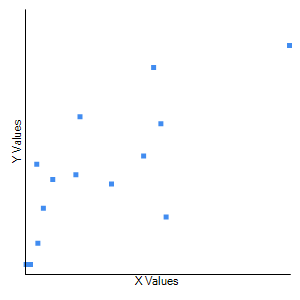
\includegraphics[scale=0.5]{Picture/One/WIPvsTP.png}}
\subfigure[WIP and Throughput feature]{\label{fig:b:1}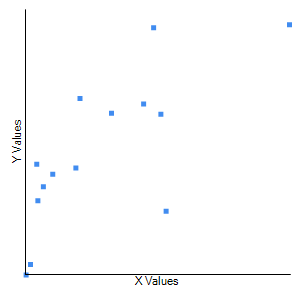
\includegraphics[scale=0.5]{Picture/One/WIPvsTPFT.png}}
\subfigure[WIP and Throughput bug]{\label{fig:c:1}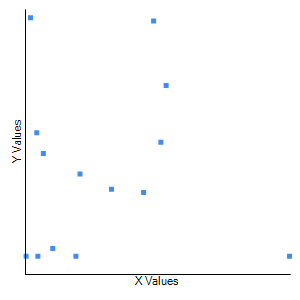
\includegraphics[scale=0.5]{Picture/One/WIPvsTPB.png}}
\caption{Correlation graphs between WIP and the throughput variables.}
\label{corr:Difference:1}
\end{figure}

\newpage


The same issue encounter for both team six and seven. In case of team six, both throughput and throughput feature have significant positive relationship with WIP while throughput bug do not. Throughput, throughput feature and throughput bug have the correlation values .64, .68 and 0.07. The total row in tables \ref{DS:Throughput:6},  \ref{DS:TPFT:6} and \ref{DS:TPB:6} shows that throughput feature consist of 609 dates and a mean value of 4.8, while throughput bug consist of 82 dates  and a mean of 3.3. The throughout variable consist of 691 dates and have a mean value of 4.58. The mean value and the number of dates strengthens the assumption that throughput feature represents more of throughput than throughput bug do.  Team four has a positive correlation between each of the variables except team size.

For team seven's case, the difference between throughput, throughput feature and throughput bug is so small, which also can be assumed by the total row in tables \ref{DS:Throughput:7},  \ref{DS:TPFT:7} and \ref{DS:TPB:7}. In the total rows, throughput has a total mean of 2.7, while throughput feature have 2.8 and throughput bug have 2.6. Throughput feature contributes 156 dates to throughput and throughput bug contributes 172 dates. The throughput correlation table in Section \ref{sec:corr:TP} proves the assumption with values of .91 for both throughput feature and bug.  

Team ten has significant positive relationship between WIP and both throughput and throughput bug. Throughput for team ten consist of 404 tasks as show in the total row in Table \ref{DS:Throughput:7}. Throughput bug represents 335 of these dates while throughput feature stands for 69 dates as shown in Tables \ref{DS:TPFT:7} and \ref{DS:TPB:7}. But the overall mean for throughput, throughput feature and throughput bug is 2.2, 2.3 and 2.2, which could reflect that these three variables have a close relationship. Both the throughput correlation table in Section \ref{sec:corr:TP} and the correlation graphs Figures in \ref{corr:Difference:10} disproves that assumption. The figure shows that the correlation dots between WIP and throughput and WIP and throughput bug is almost identical, which proves that throughput bug have a close relationship to throughput while the correlation table shows that the correlation between throughput and throughput feature is .43 which is a medium strong correlation. 


\begin{figure}[h]
\centering     %%% not \center
\subfigure[WIP and Throughput]{\label{fig:a}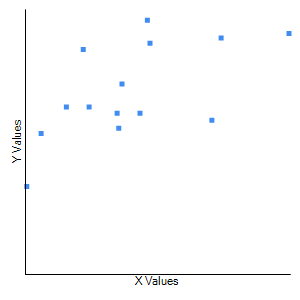
\includegraphics[scale=0.5]{Picture/Ten/WIPvsTP.png}}
\subfigure[WIP and Throughput feature]{\label{fig:b}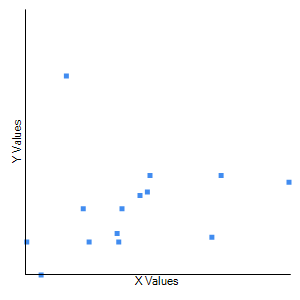
\includegraphics[scale=0.5]{Picture/Ten/WIPvsTPFT.png}}
\subfigure[WIP and Throughput bug]{\label{fig:c}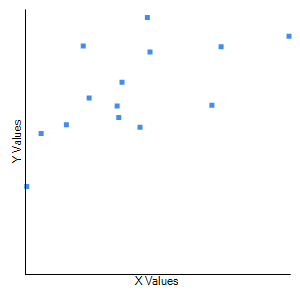
\includegraphics[scale=0.5]{Picture/Ten/WIPvsTPB.png}}
\caption{Correlation graphs between WIP and the throughput variables for team ten.}
\label{corr:Difference:10}
\end{figure}

Team one, three, four and nine have a significant positive relationship between WIP and bugs as well. For team one differ all the three churn variable from each other. Churn has a value of 0.47, churn feature has a value of .718 and churn bug of 0.15.  Judging from these variables, it will look like churn feature represents most of the churn variable. The descriptive statistic Tables \ref{DS:Churn:1}, \ref{DS:CF:1}  \ref{DS:CB:1} proves the assumption. The total mean of churn is 20.2, while churn feature has total mean of 24.5 and churn bug has a total mean of 16.8. The descriptive statistic tables also shows that churn feature contribute 150 dates to churn, while churn bug contribute 189 dates. The descriptive statistic data strengthens the assumption that both \textit{churn feature} and \textit{churn bug} represents the \textit{churn} variable. The churn correlation table in Section \ref{sec:corr:churn} proves the assumption. Both \textit{churn feature} (.566) and \textit{churn bug} (.798) have a significant positive correlation to \textit{churn}. legge inn transitive her og fiks tabeller 

%Figure \ref{corr:Difference:churn:1} states the correlation graph. The X-axis represents WIP, the Y-axis represents the churn variables.


%\begin{figure}[h]
%\centering     %%% not \center
%\subfigure[WIP and Churn]{\label{fig:a:1}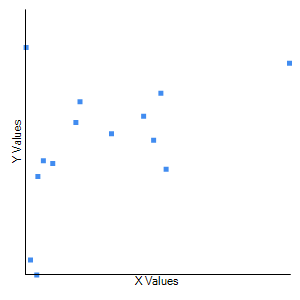
\includegraphics[scale=0.5]{Picture/One/WIPvsChurn}}
%\subfigure[WIP and Churn feature]{\label{fig:b:1}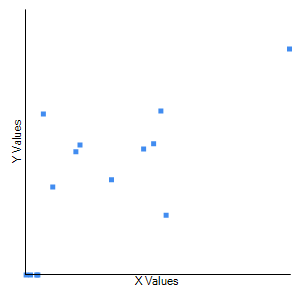
\includegraphics[scale=0.5]{Picture/One/WIPvsChurnFT.png}}
%\subfigure[WIP and Churn bug]{\label{fig:c:}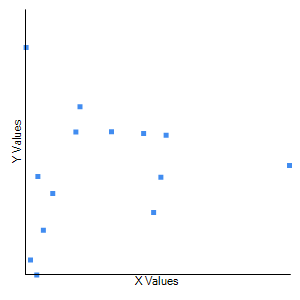
\includegraphics[scale=0.5]{Picture/One/WIPvsChurnB.png}}
%\caption{Correlation graphs between WIP and the churn variables for team one.}
%\label{corr:Difference:churn:1}
%\end{figure}



\textit{Churn} and \textit{churn bug} have a significant negative correlation in team two's case, according to the WIP correlation table. \textit{Churn feature} on the other hand has a correlation value of -0.25. According to the correlation values, one can assume that \textit{churn bug} represents most of \textit{churn}. The Tables \ref{DS:Churn:2}, \ref{DS:CF:2} and \ref{DS:CT:2} empower the assumption. \textit{Churn bug} contribute 521 dates and has a total mean value of 36.3. \textit{Churn feature} contribute 257 dates and has a mean value of 100.6. The total churn contains of 778 dates and a total mean of 57.6. The date and mean values strengthens the hypothesis. The churn correlation table in Section \ref{sec:corr:churn} proves the hypothesis. \textit{churn bug} has the value of .70 and \textit{churn feature} has the value of .58.  But both of them have a significant relationship with \textit{churn}.


In team six's case, \textit{churn bug} has a positive correlation of .77, while both \textit{churn} and \textit{churn} bug have the values of -.30 and -.36. Based on these values, the \textit{churn bug} variable represents the most of \textit{churn}. The Tables \ref{DS:Churn:6}, \ref{DS:CF:6} and \ref{DS:CT:6} backs the theory. The tables shows that \textit{churn feature} contribute 576 dates to \textit{churn} and has a total mean of 105.9. \textit{Churn bug} contains of 180 dates and has a total mean value of 73.8. The churn correlation table in Section \ref{corr.sec:churn} one can see that \textit{churn feature} has a correlation value of .98, while \textit{churn bug} has a value of -.02. These values prove the theory on contribution between the churn variables.  

The descriptive statistics tables are based on summary of the correlation values. The tables shows number of values measured(N), mean, median standard deviation(Std.dev), maximum(max)  and minimum(min) values from the correlation table.
In Table \ref{DS:corr:WIP}, the total mean of throughput is 0.6 for all the teams and the median is 0.7 , which reflects the positive correlation between WIP and throughput. The bug variables have a total mean of 0.4 with a median of 0.5, this indicates that WIP and bug have a medium strong relationship. %skrive om team size

\begin{table}[!htbp]
 \centering
 \begin{tabular}{ | l | r | r | r | r | r | r | }
 \hline
& \bf{N} & \bf{Mean} & \bf{Median} & \bf{Std.Dev} & \bf{Max} & \bf{Min} \\ \hline
Throughput  & 10 & 0.6 & 0.7 & 0.2 & 0.9 & 0.2\\ \hline
Throughput ft  & 10 & 0.5 & 0.7 & 0.3 & 0.8 & -0.1\\ \hline
Throughput bug  & 10 & 0.5 & 0.5 & 0.3 & 0.9 & 0\\ \hline
Bugs  & 10 & 0.4 & 0.5 & 0.2 & 0.7 & 0\\ \hline
Bugs finished, quarter  & 10 & 0.3 & 0.3 & 0.3 & 0.9 & -0.1\\ \hline
Avg days backlog, bugs  & 10 & 0.1 & 0.1 & 0.3 & 0.5 & -0.2\\ \hline
Lead time & 10 & 0.5 & 0.5 & 0.2 & 0.7 & 0.2\\ \hline
Churn  & 10 & 0 & 0.1 & 0.4 & 0.7 & -0.7\\ \hline
Churn ft  & 10 & 0.1 & 0.1 & 0.4 & 0.7 & -0.4\\ \hline
Churn bug  & 10 & -0 & -0 & 0.4 & 0.8 & -0.6\\ \hline
Team size  & 10 & 0.6 & 0.6 & 0.2 & 0.8 & 0.1\\ \hline
\end{tabular}
 \caption{Descriptive Statistic - Correlation - WIP}
 \label{DS:corr:WIP}
 \end{table}




\section{Correlation - Lead time}
\label{sec:corr:lt}
This section contains the correlation Table \ref{corr:Lead time}. The table shows the correlation between lead time and the variables. Team two, six and ten have significant negative relationship between lead time and churn bug. The churn and churn bug variables for team two have the correlation values of  -0.45 and -.73. These values are relative close.  However, churn feature have a value of 0.41. The total row in tables \ref{DS:Churn:2}, \ref{DS:CF:2} and \ref{DS:CB:2} shows that churn for team two consist of 1572 dates. Churn feature consist of 375 dates and churn bug of 1197 dates. Churn bug contribute 76\%  (1197/1572) of the total amount of dates in churn. The total mean of churn, churn feature and churn bug is 65.7, 111.4 and 51.3, which could reflect that churn bug contribute more to the churn variable than churn feature. The churn correlation table in Section \ref{sec:corr:churn} with the correlation value of .08 for churn feature and .728 for churn bug, states that churn bug represents the most of the churn variable. Team two also has significant negative relationship between lead time and the bugs finished, quarter variable.

For team six, Churn bug has a negative correlation of -.55 while churn has a correlation of -0.08 and churn feature a correlation of -0.2. The reason why churn bug differ from churn is because churn bug consist of 17\% (265/1533) of the churn dates as shown in tables \ref{DS:Churn:6} and \ref{DS:CB:6}. The two tables and Table \ref{DS:CF:6} also shows the total mean of churn is 146, while the total mean for churn feature is 156.5 and for churn bug it's 95.2. With the total mean, one can assume that churn bug don't contribute too much to the churn variable, hence big difference between the two mean values. The assumption is proved by the churn correlation table in Section \ref{sec:corr:churn} with the values .980 for churn feature and .018 for churn bug. Throughput bug also differ from throughput for team six. The reason why where explained in section \ref{corr:WIP}.
\begin{table}[!htbp]
 \begin{adjustwidth}{-2.5cm}{}
 \centering
 \begin{tabular}{|l|r|r|r|r|r|r|r|r|r|r|}
\hline
 & \bf{T1} & \bf{T2} & \bf{T3} & \bf{T4} & \bf{T5} & \bf{T6} & \bf{T7} & \bf{T8} & \bf{T9} & \bf{T10}\\ \hline
WIP &.749**& 0.46& 0.49& .704**& .566*& 0.29& .678*& 0.16& 0.23& .719**\\ \hline
Throughput &.700**& .673**& 0.49& .677**& 0.36& 0.13& 0.47& 0.54& 0.42& 0.32\\ \hline
Throughput Feature &.733**& 0.09& 0.44& .644*& 0.14& 0.10& 0.41& .621*& 0.41& -0.05\\ \hline
Throughput bug &-0.30& .596*& 0.52& .644*& 0.42& -0.01& 0.61& -0.17& 0.28& 0.37\\ \hline
Bugs &.767**& 0.50& .536*& 0.31& 0.32& -0.23& .692*& -0.13& 0.44& 0.04\\ \hline
Bugs finished, quarter &.697**& -0.14& 0.20& 0.23& -0.09& -0.27& .731*& 0.37& 0.53& 0.19\\ \hline
Avg days in backlog, bugs &0.06& 0.40& 0.07& 0.07& -0.08& -0.03& 0.57& -0.12& -0.48& -0.52\\ \hline
Churn &.700**& -0.42& -0.45& .973**& 0.18& -0.34& 0.39& .908**& -0.37& -0.04\\ \hline
Churn feature &.858**& 0.20& -0.27& .964**& 0.11& -0.31& 0.39& .786**& -0.46& 0.32\\ \hline
Churn bug &0.26& -0.39& -.637*& 0.20& 0.24& 0.28& -0.05& -0.12& -0.08& -0.27\\ \hline
Team size &.607*
& 0.38& 0.44& -0.30& 0.36& -0.11& 0.59& 0.22& 0.38& 0.53\\ \hline
\end{tabular}
 \caption{Correlation - Lead time}
 \label{corr:Lead time}
 \centerline {* Correlation is significant at the 0.05 level (2-tailed).}
\centerline{** Correlation is significant at the 0.01 level (2-tailed).}
\centerline{c. Cannot be computed because at least one of the variables is constant.}
\end{adjustwidth}
\end{table}
\newpage


Both churn bug and churn for team ten have a significant negative relationship with lead time, but churn feature don't. The Tables \ref{DS:Churn:10}, \ref{DS:CF:10} and \ref{DS:CB:10} shows the total mean of churn is 50.4, the total of churn feature its 66 and for churn bug its 47.7. In case of the mean values, it looks like churn bug has a close relationship with churn. Churn bug also consist of 85\% of the overall dates in churn (517/609) which supports the assumption that churn bug consist of much of the churn variable. The assumption is proven right by the churn correlation table in \ref{sec:corr:churn} and correlation graphs in Figure \ref{corr:Difference:lt}. The figure shows the lead time in the X-axis and the churn variable in the Y-axis. One can clearly see that Figures \ref{fig:a:lt:10} and \ref{fig:c:lt:10} have a significant negative correlation with lead time. The dot pattern in these two figures is also similar, which points to the case that churn and churn bug are alike and that churn feature don't represents of much of the churn nor have a close relationship to churn. 


\begin{figure}[h]
\centering     %%% not \center
\subfigure[Lead time and Churn]{\label{fig:a:lt:10}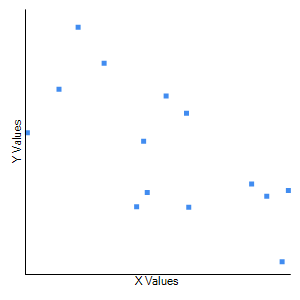
\includegraphics[scale=0.5]{Picture/Ten/LTvsChrn.png}}
\subfigure[Lead time and Churn feature]{\label{fig:b:lt:10}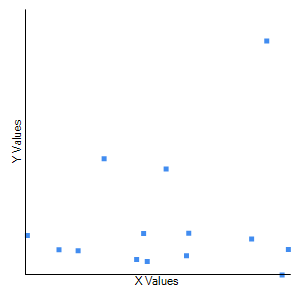
\includegraphics[scale=0.5]{Picture/Ten/LTvsChrnFT.png}}
\subfigure[Lead time and Churn bug]{\label{fig:c:lt:10}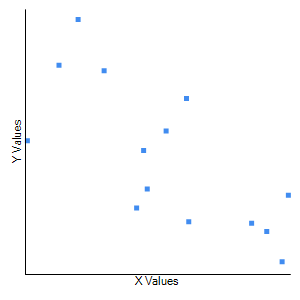
\includegraphics[scale=0.5]{Picture/Ten/LTvsChrnB.png}}
\caption{Correlation graphs between lead time and churn variables for team ten.}
\label{corr:Difference:lt}
\end{figure}

The descriptive statistic table for lead time shown in Table \ref{DS:corr:LT} shows that there is no value with overall significant relationship with lead time. 
\begin{table}[!htbp]
 \centering
 \begin{tabular}{ | l | r | r | r | r | r | r | }
 \hline
 & \bf{N} & \bf{Mean} & \bf{Median} & \bf{Std.Dev} & \bf{Max} & \bf{Min} \\ \hline
WIP  & 10 & 0.5 & 0.5 & 0.2 & 0.7 & 0.2\\ \hline
Throughput  & 10 & 0.5 & 0.5 & 0.2 & 0.7 & 0.1\\ \hline
Throughput ft  & 10 & 0.4 & 0.4 & 0.3 & 0.7 & -0.1\\ \hline
Throughput bug  & 10 & 0.3 & 0.4 & 0.3 & 0.6 & -0.3\\ \hline
Bugs  & 10 & 0.3 & 0.4 & 0.3 & 0.8 & -0.2\\ \hline
Bugs finished, quarter  & 10 & 0.2 & 0.2 & 0.3 & 0.7 & -0.3\\ \hline
Avg days backlog, bugs  & 10 & -0 & 0 & 0.3 & 0.6 & -0.5\\ \hline
Churn  & 10 & 0.2 & 0.1 & 0.6 & 1 & -0.5\\ \hline
Churn ft  & 10 & 0.3 & 0.3 & 0.5 & 1 & -0.5\\ \hline
Churn bug  & 10 & -0.1 & -0.1 & 0.3 & 0.3 & -0.6\\ \hline
Team size  & 10 & 0.3 & 0.4 & 0.3 & 0.6 & -0.3\\ \hline
\end{tabular}
 \caption{Descriptive Statistic - Correlation - Lead time}
 \label{DS:corr:LT}
 \end{table}


\section{Correlation - Bugs}
\label{sec:corr:bug}
This section contains information about the correlation table between the variables and bugs. The result is listed in Table \ref{corr:bug}. Teams one, two, three, four, five, nine and ten all have a significant positive correlation between bugs and throughput. For team three, four, five and nine's case, all throughput variables have a significant positive correlation with bugs. For team one and ten, the throughput  relationship differ. The reason why where stated in Section \ref{sec:corr:WIP}. 
\begin{table}[!htbp]
 \begin{adjustwidth}{-1.5cm}{}
 \centering
 \begin{tabular}{|l|r|r|r|r|r|r|r|r|r|r|}
\hline
 &  \bf{T1} & \bf{T2} & \bf{T3} & \bf{T4} & \bf{T5} & \bf{T6} & \bf{T7} & \bf{T8} & \bf{T9} & \bf{T10}\\ \hline
WIP &.725**& 0.20& .599*& .560*& 0.50& 0.46& 0.62& 0.04& .581*& 0.18\\ \hline
Throughput &.687**& .810**& .880**& .586*& .975**& 0.27& 0.53& 0.41& .699**& .557*\\ \hline
Throughput Feature &.738**& 0.01& .822**& .583*& .881**& 0.30& 0.56& 0.22& .597*& -0.14\\ \hline
Throughput bug &-0.17& .834**& .868**& .583*& .959**& .686**& 0.50& .915**& .653*& .589*\\ \hline
Bugs finished, quarter &0.50& -0.18& 0.12& 0.40& 0.17& .762**& .785**& 0.18& .701**& 0.05\\ \hline
Avg days in backlog, bugs &0.52& 0.38& 0.43& 0.30& 0.18& 0.24& 0.23& 0.28& 0.21& 0.13\\ \hline
Leadtime &-0.23& -0.23& -0.24& 0.25& -0.25& -0.22& 0.54& -0.12& -0.06& -0.14\\ \hline
Churn &0.23& -0.01& 0.00& .c& -0.17& -0.10& 0.19& -0.08& -0.34& 0.31\\ \hline
Churn feature &0.30& 0.07& -0.03& .c& 0.28& -0.04& 0.13& -0.15& -.618*& 0.06\\ \hline
Churn bug &0.37& 0.17& -0.08& .c& -0.19& 0.43& 0.14& 0.04& 0.10& 0.28\\ \hline
Team size & .803**
& 0.26& 0.27& 0.17& .711**
& 0.41& 0.41& 0.42& 0.41& 0.16\\ \hline
\end{tabular}
 \caption{Correlation - Bugs}
 \label{corr:bug}
 \centerline {* Correlation is significant at the 0.05 level (2-tailed).}
\centerline{** Correlation is significant at the 0.01 level (2-tailed).}
\centerline{c. Cannot be computed because at least one of the variables is constant.}
\end{adjustwidth}
\end{table}





Team two's Throughput feature differ from throughput. One could believe that the reason is that throughput bug consists of 2/3 of the throughput variable (460/690) as shown in the descriptive statistic Tables \ref{DS:Throughput:2} and \ref{DS:TPB:2}. But the two tables and table \ref{DS:TPFT:2} shows that the total mean of throughput is 4.39. While for throughput bug it's 4.8 and 3.7 for throughput feature. These three variables are quiet close, which could reflect that these three variables should be close based on correlation measurement. But, the Figures in \ref{corr:Difference:2} and the throughput correlation table in \ref{sec:corr:TP} shows that they are not. The Figure \ref{corr:Difference:2} shows the bugs variable in the X-axis and the throughput variable in the Y-axis. Both Figures \ref{fig:a:2} and \ref{fig:c:2} shows a significant positive correlation. But for Figure \ref{fig:b:2} one can see that the dots are more randomly placed. For example, when the Y value is at vertex, x value is low.  When x is at vertex, y values are both low and high.  

\begin{figure}[h]
\centering     %%% not \center
\subfigure[Bugs and Throughput]{\label{fig:a:2}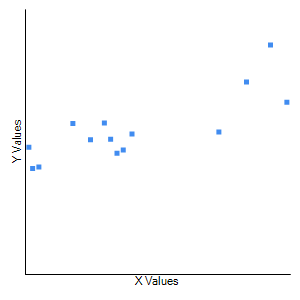
\includegraphics[scale=0.5]{Picture/Two/BugVSTP.png}}
\subfigure[Bugs and Throughput feature]{\label{fig:b:2}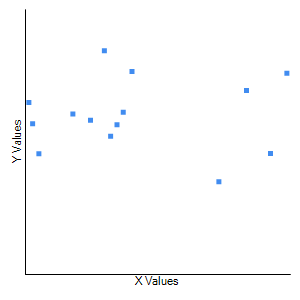
\includegraphics[scale=0.5]{Picture/Two/BugVSTPFT.png}}
\subfigure[Bugs and Throughput bug]{\label{fig:c:2}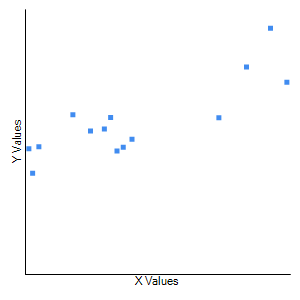
\includegraphics[scale=0.5]{Picture/Two/BugVSTPB.png}}
\caption{Correlation graphs between bugs and the throughput variables.}
\label{corr:Difference:2}
\end{figure}
\newpage

Team six and nine have a significant positive correlation between the variable Bugs finished, quarter. Team nine also has a significant negative correlation between bug and churn feature, but not churn. Churn feature consist of approximately 1/3 (295/923) of the churn variable as shown in Tables \ref{DS:Churn:9} and \ref{DS:CF:9}.  The total mean of churn feature is 133.9, the total mean for churn is 81.9 and the total mean for churn bug is 57.5, as shown in the previous stated tables and Table \ref{DS:CB:10}. The correlation graphs in Figure \ref{corr:Difference:9}, show the bugs variable in the X-axis and churn variable in the Y-axis. The figure shows that there is neither a significant negative nor significant positive pattern between either bug and churn nor bug and churn bug. The Figure \ref{fig:b:9} however, shows that there is a vaguely significant negative correlation between bug and churn. Even though churn feature have a significant correlation to a variable, and the churn do not, does not say that churn feature can't have a significant positive correlation to churn. The correlation table for churn in Section \ref{sec:corr:churn} shows that both churn feature and churn bug for team nine have a significant correlation with churn. Judging from the Figure \ref{corr:Difference:9} and the correlation table from Section \ref{sec:corr:churn} one can assume that correlation is not transitive. The paper "The Non-Transitivity of Pearson's Correlation Coefficient: An Educational Perspective" \parencite{corr:transitive} proves the assumption. 

 


\begin{figure}[h]
\centering     %%% not \center
\subfigure[Bug and Churn]{\label{fig:a:9}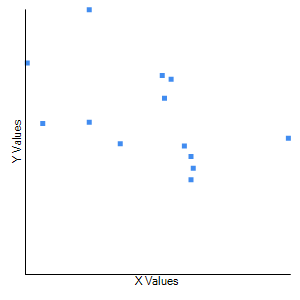
\includegraphics[scale=0.5]{Picture/Nine/BugsVSChrn.png}}
\subfigure[Bug and Churn feature]{\label{fig:b:9}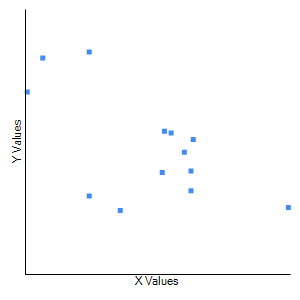
\includegraphics[scale=0.5]{Picture/Nine/BugsVSChrnFT.png}}
\subfigure[Bug and Churn bug]{\label{fig:c:9}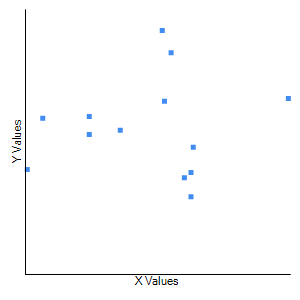
\includegraphics[scale=0.5]{Picture/Nine/BugsVSChrnB.png}}
\caption{Correlation graphs between bug and the churn variables for team nine.}
\label{corr:Difference:9}
\end{figure}



In Table \ref{DS:corr:Bugs}, one can see that WIP with a mean value of 0.4 have a medium correlation with bugs as stated in Section \ref{corr:WIP}.  Throughput  have a value of 0.6. This shows that throughput have a high correlation with bugs.

\begin{table}[!htbp]
 \centering
 \begin{tabular}{ | l | r | r | r | r | r | r | }
 \hline
& \bf{N} & \bf{Mean} & \bf{Median} & \bf{Std.Dev} & \bf{Max} & \bf{Min} \\ \hline
WIP  & 10 & 0.4 & 0.5 & 0.2 & 0.7 & 0\\ \hline
Throughput  & 10 & 0.6 & 0.6 & 0.2 & 1 & 0.3\\ \hline
Throughput ft  & 10 & 0.5 & 0.6 & 0.3 & 0.9 & -0.1\\ \hline
Throughput bug  & 10 & 0.6 & 0.7 & 0.3 & 1 & -0.2\\ \hline
Bugs finished, quarter  & 10 & 0.3 & 0.3 & 0.3 & 0.8 & -0.2\\ \hline
Avg days backlog, bugs  & 10 & 0.3 & 0.3 & 0.1 & 0.5 & 0.1\\ \hline
Lead time & 10 & 0.3 & 0.4 & 0.3 & 0.8 & -0.2\\ \hline
Churn  & 10 & 0 & -0 & 0.3 & 0.6 & -0.5\\ \hline
Churn ft  & 10 & 0.1 & 0.1 & 0.4 & 0.8 & -0.6\\ \hline
Churn bug  & 10 & 0 & 0 & 0 & 0.6 & -0\\ \hline
Team size  & 10 & 0.3 & 0.4 & 0.3 & 0.6 & -0.3\\ \hline
\end{tabular}
 \caption{Descriptive Statistic - Correlation - Bugs}
 \label{DS:corr:Bugs}
 \end{table}


\section {Correlation - Throughput}
\label{sec:corr:TP}
This section shows the correlation table between throughput and the variables. The result is listed in Table \ref{corr:TP}. Throughput has a significant correlation to either throughput feature or throughput bug for each of the teams. For team three, four, five, seven and nine, both the sub variables of throughput have significant positive correlation to throughput. For team one and six, throughput feature differ from throughput, the reason where explained in Section \ref{sec:corr:WIP}.   The Section \ref{sec:corr:WIP} also explain the reason throughput bug differ from throughput for team ten.    Throughput feature differ from throughput for team two and the reason for that is stated in section \ref{sec:corr:bug}.

\begin{table}[!htbp]
 \begin{adjustwidth}{-1.5cm}{}
 \centering
 \begin{tabular}{|l|r|r|r|r|r|r|r|r|r|r|}
\hline
 & \bf{T1} & \bf{T2} & \bf{T3} & \bf{T4} & \bf{T5} & \bf{T6} & \bf{T7} & \bf{T8} & \bf{T9} & \bf{T10}\\ \hline
WIP &.743**& 0.21& .756**& .826**& 0.52& .638*& .674*& 0.47& .893**& .612*\\ \hline
Throughput Feature &.956**& 0.09& .933**& .997**& .854**& .995**& .912**& .940**& .882**& 0.43\\ \hline
Throughput bug &0.03& .970**& .986**& .997**& .994**& 0.04& .908**& 0.44& .960**& .980**\\ \hline
Bugs &.687**& .810**& .880**& .586*& .975**& 0.27& 0.53& 0.41& .699**& .557*\\ \hline
Bugs finished, quarter &0.16& 0.12& 0.23& 0.39& 0.12& 0.12& 0.58& 0.33& .696**& .589*\\ \hline
Avg days in backlog, bugs &0.16& 0.12& 0.45& 0.37& 0.14& -0.17& 0.21& -0.17& -0.41& -0.09\\ \hline
Leadtime &.700**& .673**& 0.49& .677**& 0.36& 0.13& 0.47& 0.54& 0.42& 0.32\\ \hline
Churn &0.37& -0.43& -0.18& .725**& -0.06& -0.40& 0.43& .594*& -0.14& 0.02\\ \hline
Churn feature &.776**& -0.10& -0.20& .806**& 0.41& -0.40& 0.43& 0.43& -0.29& -0.20\\ \hline
Churn bug &-0.06& -0.21& -0.33& 0.49& -0.10& .567*& -0.37& 0.03& -0.29& -0.06\\ \hline
Team size &.699**
& 0.05& 0.52& 0.16& .687**
& .858**
& 0.62& .753**
& 0.53& .\\ \hline
\end{tabular}
 \caption{Correlation - Throughput}
 \label{corr:TP}
 \centerline {* Correlation is significant at the 0.05 level (2-tailed).}
\centerline{** Correlation is significant at the 0.01 level (2-tailed).}
\centerline{c. Cannot be computed because at least one of the variables is constant.}
\end{adjustwidth}
\end{table}

Both team nine and ten have a positive significant correlation between bug and the Bugs finished, quarter variable. Team six have a significant correlation between bugs and churn bug. The reason churn bug differ from churn and churn feature where stated in Section \ref{sec:corr:lt}. Team seven has a significant positive correlation between throughput and the variables churn and churn bug, but not churn feature, but churn feature has almost a significant positive correlation.  Churn feature consist of 235, churn bug consist of 417 and churn of 652 dates. The mean values for the three variables are 148.1 for churn feature, 68.4 for churn bug and 91.1 for churn. An indication of these variables are that both churn feature and churn bug contribute to the churn variables, hence the mean values. The correlation table for churn in section \ref{sec:corr:churn} proves the assumption.  Churn feature and churn bug have a positive correlation with churn. This is another example of transitivity and correlation as stated in Section \ref{sec:corr:bug}.


For team eight, throughput bug differ from throughput. Throughput bug consist of 99 dates and have total mean of 1.5. Throughput feature consist of 92 dates and a mean of 3.2. While throughput have a mean of 2.3. These numbers are gathered from the descriptive statistic Tables \ref{DS:Throughput:8}, \ref{DS:TPFT:8} and \ref{DS:TPB:8}.  On the basis of these numbers it will look like both of the sub variables of throughput contributes and both of them should have close relationship to throughput.  But, in Figure \ref{corr:Difference:8} the difference are stated. The Figure \ref{corr:Difference:8} shows the throughput variable in the X-axis and the sub variables in the Y-axis. In Figure \ref{fig:a:8}, the dots are clearly moving in a upwards direction, while in Figure \ref{fig:b:8} almost all the dots are all gathered around the low values of Y.

\begin{figure}[h]
\centering     %%% not \center
\subfigure[Throughput and Throughput feature]{\label{fig:a:8}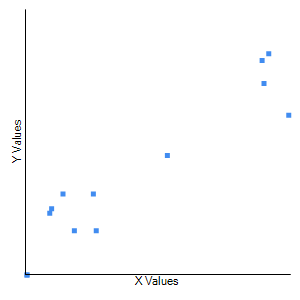
\includegraphics[scale=0.5]{Picture/Eight/TPvsTPFT.png}}
\subfigure[Throughput and Throughput bug]{\label{fig:b:8}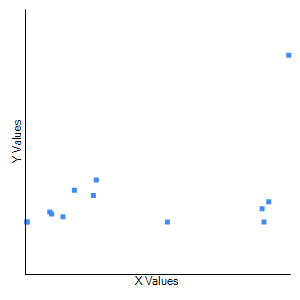
\includegraphics[scale=0.5]{Picture/Eight/TPvsTPB.png}}
\caption{Correlation graphs between the throughput variables.}
\label{corr:Difference:8}
\end{figure}



 
Team eight also has a significant negative correlation between throughput and churn. Churn has a negative value of -.64, while churn feature has a value of -0.45 and churn bug has a value of -0.28. Churn feature consist of 246 of the 329 dates, as shown in Tables \ref{DS:Churn:8} and \ref{DS:CF:8}. The Table \ref{DS:CF:8} also shows that churn feature mostly consist of tasks that requires zero churn. The total mean of these three values are 0.9 for churn, 0.1 for churn feature and 3.6 for churn bug as shown in the Tables   \ref{DS:Churn:8}, \ref{DS:CF:8} and \ref{DS:CB:8}. The zeros from churn feature play a part in the mean value of churn. But, in the correlation for churn in section \ref{sec:corr:churn}, one can see that churn bug have a significant correlation with churn, while churn feature don't. So the contribution of the churn feature's mean in the case of correlation between throughput and churn made enough impact for churn to have a significant correlation with throughput.

According to Table \ref{DS:corr:TP}, bugs have a strong positive correlation with throughput as stated Section \ref{sec:corr:bug}. WIP have a medium positive relationship with throughput which where stated in \ref{sec:corr:WIP}. The sub variables throughput feature (0.6) and throughput bug (0.4) have respectively a strong and medium relationship to throughput. 

\begin{table}[!htbp]
 \centering
 \begin{tabular}{ | l | r | r | r | r | r | r | }
 \hline
& \bf{N} & \bf{Mean} & \bf{Median} & \bf{Std.Dev} & \bf{Max} & \bf{Min} \\ \hline
WIP  & 10 & 0.6 & 0.7 & 0.2 & 0.9 & 0.2\\ \hline
Throughput ft  & 10 & 0.8 & 0.9 & 0.3 & 1 & 0.1\\ \hline
Throughput bug  & 10 & 0.7 & 1 & 0.4 & 1 & 0\\ \hline
Bugs  & 10 & 0.6 & 0.6 & 0.2 & 1 & 0.3\\ \hline
Bugs finished, quarter  & 10 & 0.3 & 0.3 & 0.2 & 0.7 & 0.1\\ \hline
Avg days backlog, bugs  & 10 & 0.1 & 0.1 & 0.3 & 0.5 & -0.4\\ \hline
Lead time & 10 & 0.5 & 0.5 & 0.2 & 0.7 & 0.1\\ \hline
Churn  & 10 & 0.1 & -0 & 0.4 & 0.7 & -0.4\\ \hline
Churn ft  & 10 & 0.2 & 0.2 & 0.5 & 0.8 & -0.4\\ \hline
Churn bug  & 10 & -0 & -0.1 & 0.3 & 0.6 & -0.4\\ \hline
Team size  & 10 & 0.5 & 0.6 & 0.3 & 0.9 & 0.1\\ \hline
\end{tabular}
 \caption{Descriptive Statistic - Correlation - Throughput}
 \label{DS:corr:TP}
 \end{table}

\section{Correlation - Churn}
\label{sec:corr:churn}
This section contains information about the correlation table between the variables and churn. The result is listed in Table \ref{corr:churn}.  All teams with valid churn have either one or both churn variable with significant positive correlation with churn. Teams two, five, six eight and ten don't have a positive correlation between both the churn variables and churn.  

\begin{table}[!htbp]
 \begin{adjustwidth}{-1.5cm}{}
 \centering
 \begin{tabular}{|l|r|r|r|r|r|r|r|r|r|r|}
\hline
 & \bf{T1} & \bf{T2} & \bf{T3} & \bf{T4} & \bf{T5} & \bf{T6} & \bf{T7} & \bf{T8} & \bf{T9} & \bf{T10}\\ \hline
WIP &0.47& -.709**& -0.32& .656*& 0.03& -0.30& 0.10& 0.16& -0.09& 0.16\\ \hline
Throughput &0.37& -0.43& -0.18& .725**& -0.06& -0.40& 0.43& .594*& -0.14& 0.02\\ \hline
Throughput Feature &0.36& 0.00& -0.12& .689**& -0.03& -0.37& 0.45& .632*& 0.02& -0.17\\ \hline
Throughput bug &-0.52& -0.42& -0.22& .689**& -0.03& -0.03& 0.54& -0.17& -0.20& 0.07\\ \hline
Bugs &.617*& -0.27& 0.10& 0.27& -0.06& -0.12& 0.11& -0.16& -0.48& 0.04\\ \hline
Bugs finished, quarter &.804**& -0.22& -0.11& 0.15& -0.31& 0.04& 0.17& 0.49& -0.05& 0.31\\ \hline
Avg days in backlog, bugs &0.19& -0.12& -0.06& 0.00& 0.15& .557*& 0.60& -0.17& -0.01& -0.11\\ \hline
Leadtime &.700**& -0.42& -0.45& .973**& 0.18& -0.34& 0.39& .908**& -0.37& -0.04\\ \hline
Churn feature &.566*& .584*& .901**& .988**& 0.22& .977**& 1.000**& .838**& .619*& 0.14\\ \hline
Churn bug &.798**& .699**& .846**& 0.13& .943**& -0.02& -0.10& -0.07& 0.39& .938**\\ \hline
Team size &0.42& -0.16& -0.51& -0.24& -.541*
& -0.18& 0.36& 0.14& 0.11& 0.12\\ \hline
\end{tabular}
 \caption{Correlation - Churn}
 \label{corr:churn}
 \centerline {* Correlation is significant at the 0.05 level (2-tailed).}
\centerline{** Correlation is significant at the 0.01 level (2-tailed).}
\centerline{c. Cannot be computed because at least one of the variables is constant.}
\end{adjustwidth}
\end{table}


For team two and ten's case, churn feature differ from churn, the reason where stated in Section \ref{sec:corr:lt}. Section \ref{sec:corr:lt} also states the reason churn bug differ from churn in the case of team six is. Team five on the other hand,  has a significant positive correlation between churn and churn bug, but not for churn feature.  Churn feature consist of approximately 10\% (182/1901) of the total churn dates as shown in Tables \ref{DS:Churn:5} and \ref{DS:CF:5}. The two previous stated tables and Table \ref{DS:CB:5} shows that churn has a mean value of 23.5, churn feature has a mean value of 43.1 and churn bug with a mean value of 21.4. These values show that churn feature don't represent much of the churn variable. 

Team eight has a significant positive correlation between churn and churn bug and almost churn feature. Churn feature consist of approximately 75\% (246/329) of all churn dates as shown in Tables \ref{DS:Churn:8} and \ref{DS:CF:8}. But as stated in in \ref{sec:corr:TP}, almost each of the churn feature task requires zero churn, and with zero churn, its hard to make an impact on the overall churn. 

Table \ref{DS:corr:Churn} shows both churn feature and churn have a close relationship with churn
\begin{table}[!htbp]
 \centering
 \begin{tabular}{ | l | r | r | r | r | r | r | }
 \hline
& \bf{N} & \bf{Mean} & \bf{Median} & \bf{Std.Dev} & \bf{Max} & \bf{Min} \\ \hline
WIP  & 10 & 0 & 0.1 & 0.4 & 0.7 & -0.7\\ \hline
Throughput  & 10 & 0.1 & -0 & 0.4 & 0.7 & -0.4\\ \hline
Throughput ft  & 10 & 0.1 & 0 & 0.4 & 0.7 & -0.4\\ \hline
Throughput bug  & 10 & -0 & -0.1 & 0.4 & 0.7 & -0.5\\ \hline
Bugs  & 10 & 0 & -0 & 0.3 & 0.6 & -0.5\\ \hline
Bugs finished, quarter  & 10 & 0.1 & 0.1 & 0.3 & 0.8 & -0.3\\ \hline
Avg days backlog, bugs  & 10 & 0.1 & -0 & 0.3 & 0.6 & -0.2\\ \hline
Lead time & 10 & 0.2 & 0.1 & 0.6 & 1 & -0.5\\ \hline
Churn ft  & 10 & 0.7 & 0.7 & 0.3 & 1 & 0.1\\ \hline
Churn bug  & 10 & 0.5 & 0.5 & 0.4 & 0.9 & -0.1\\ \hline
Team size  & 10 & -0 & -0 & 0.3 & 0.4 & -0.5\\ \hline
\end{tabular}
 \caption{Descriptive Statistic - Correlation - Churn}
 \label{DS:corr:Churn}
 \end{table}
 
 \section{Team size}
 \begin{table}[!htbp]
  \begin{adjustwidth}{-2.5cm}{}
 \centering
 \begin{tabular}{|l|r|r|r|r|r|r|r|r|r|r|}
\hline
 & \bf{T1} & \bf{T2} & \bf{T3} & \bf{T4} & \bf{T5} & \bf{T6} & \bf{T7} & \bf{T8} & \bf{T9} & \bf{T10}\\ \hline
WIP &.684**& 0.35& .778**& 0.06& .575*& .767**& 0.62& .651*& 0.54& .759**\\ \hline
Throughput &.699**& 0.05& 0.52& 0.16& .687**& .858**& 0.62& .753**& 0.53& .573*\\ \hline
Throughput Feature &.736**& -0.22& 0.53& 0.20& 0.48& .893**& 0.47& .745**& 0.48& 0.18\\ \hline
Throughput bug &-0.10& 0.06& 0.51& 0.20& .673**& 0.00& .715*& 0.40& 0.48& .637*\\ \hline
Bugs & .803**& 0.26& 0.27& 0.17& .711**& 0.41& 0.41& 0.42& 0.41& 0.16\\ \hline
Bugs finished, quarter &0.42& -0.53& 0.25& -0.19& 0.28& 0.30& .711*& 0.05& 0.38& 0.34\\ \hline
Avg days in backlog, bugs &0.48& .841**& 0.04& 0.44& 0.03& -0.03& 0.49& 0.03& 0.07& -0.03\\ \hline
Leadtime &.607*& 0.38& 0.44& -0.30& 0.36& -0.11& 0.59& 0.22& 0.38& 0.53\\ \hline
Churn &0.42& -0.16& -0.51& -0.24& -.541*& -0.18& 0.36& 0.14& 0.11& 0.12\\ \hline
Churn feature &.786**& 0.41& -0.42& -0.17& 0.32& -0.23& 0.36& 0.07& 0.01& 0.36\\ \hline
Churn bug &0.26& -0.44& -.606*& 0.27& -.552*& .741**& -0.32& -0.14& -0.16& -0.10\\ \hline
\end{tabular}
 \caption{Correlation - Leadtime}
 \label{corr:Teams}
 \centerline {* Correlation is significant at the 0.05 level (2-tailed).}
\centerline{** Correlation is significant at the 0.01 level (2-tailed).}
\centerline{c. Cannot be computed because at least one of the variables is constant.}
\end{adjustwidth}
\end{table}
 
 
\begin{table}[!htbp]
 \centering
 \begin{tabular}{ | l | r | r | r | r | r | r | }
 \hline
& \bf{N} & \bf{Mean} & \bf{Median} & \bf{Std.Dev} & \bf{Max} & \bf{Min} \\ \hline
WIP  & 10 & 0.6 & 0.6 & 0.2 & 0.8 & 0.1\\ \hline
Throughput  & 10 & 0.5 & 0.6 & 0.3 & 0.9 & 0.1\\ \hline
Throughput ft  & 10 & 0.4 & 0.5 & 0.3 & 0.9 & -0.2\\ \hline
Throughput bug  & 10 & 0.4 & 0.4 & 0.3 & 0.7 & -0.1\\ \hline
Bugs  & 10 & 0.4 & 0.4 & 0.2 & 0.8 & 0.2\\ \hline
Bugs finished, quarter  & 10 & 0.2 & 0.3 & 0.3 & 0.7 & -0.5\\ \hline
Avg days backlog, bugs  & 10 & 0.2 & 0.1 & 0.3 & 0.8 & -0\\ \hline
Lead time & 10 & 0.3 & 0.4 & 0.3 & 0.6 & -0.3\\ \hline
Churn  & 10 & -0 & -0 & 0.3 & 0.4 & -0.5\\ \hline
Churn ft  & 10 & 0.1 & 0.2 & 0.4 & 0.8 & -0.4\\ \hline
Churn bug  & 10 & -0.1 & -0.1 & 0.4 & 0.7 & -0.6\\ \hline
\end{tabular}
 \caption{Descriptive Statistic - Correlation - Throughput}
 \label{DS:corr:TP}
 \end{table}
 
 \chapter{Discussion}
 \label{ch:discussion} 
 \section{swag}
 The research on kanban says you should limit WIP to increase throughput and decrease lead time. According to the Table \ref{DS:corr:WIP}, throughput increases when WIP increases for in average for all the teams.  Six out of ten teams have a significant positive correlation between WIP and throughput. One could argue, when throughput decreases, bug also decreases according to Table \ref{DS:corr:TP}. That may not be the case. When one produces more tasks, more bugs are produced. The Table \ref{DS:corr:WIP} shows that WIP and bugs have a medium relationship. Out of the six teams with a positive correlation between WIP and throughput, four has a significant positive correlation between WIP and bugs. The correlation values are not transitive as said in Section \ref{sec:corr:bug}, but that don't mean that there is no relationship between the WIP correlation and the throughput correlation. 
 
In WIP's correlation table (\ref{corr:WIP}) team four and team nine is the two teams with strongest correlation between throughput and WIP. Team four has the correlation value of .83 and team nine has the value of .89. Over the three year period the data was recorded, team four had the total of 63 employees while team nine had 109 as shown by Tables \ref{team:4} and \ref{team:9}. 



Over the period, team four is the team with fewest employees and team one with 330 is the team with highest employees, shown in Table \ref{table:teams}.   
 
 
  T1(330-W:20.5),3(135),5(285),6(99),8(162) and 10(170) team vs wip = sig
2(150- W:23.8),4(63),7(76),9(109) wip = not sig 

The teams one, three, five, six, eight and ten have a significant positive correlation between WIP and team size shown in Table \ref{corr:Teams}.  Both team seven and nine is close to have significant positive relationship with the values of 0.62 and 0.54. Four out of the six teams represents the four highest teams based on team size, while two of the teams without a significant correlation represent the two lowest teams based on team size as shown in Table \ref{table:teams}. Team seven represents one of these teams.  
 
 \begin{appendices}
\chapter{Descriptive statistics for the ten teams}
\label{app:DS}
 
\section{Team 1 - Descriptive Statistics}
\begin{table}[!htbp]
  \begin{adjustwidth}{-2.5cm}{}
\subfigure[Descriptive Statistic -WIP]{
 \label{DS:WIP:1}
 \scalebox{0.85}{
  \begin{tabular}{ | l | r | r | r | r | r | r | }
 \hline
 Quarter &	N &	Mean &	Median & Std.Dev & Max	& Min \\ \hline
2010-3  & 25.0 & 3.6 & 4.0 & 0.6 & 5.0 & 3.0\\ \hline
2010-4 & 92.0 & 0.7 & 1.0 & 0.7 & 3.0 & 0\\ \hline
2011-1 & 90.0 & 3.4 & 1.0 & 6.9 & 30.0 & 0\\ \hline
2011-2 & 91.0 & 13.2 & 4.0 & 14.5 & 51.0 & 2.0\\ \hline
2011-3 & 92.0 & 1.8 & 2.0 & 0.6 & 3.0 & 1.0\\ \hline
2011-4 & 92.0 & 14.3 & 4.0 & 22.7 & 97.0 & 1.0\\ \hline
2012-1 & 91.0 & 22.2 & 21.0 & 14.5 & 67.0 & 4.0\\ \hline
2012-2 & 91.0 & 30.3 & 23.0 & 29.0 & 107.0 & 9.0\\ \hline
2012-3 & 92.0 & 36.0 & 38.5 & 13.6 & 65.0 & 18.0\\ \hline
2012-4 & 92.0 & 34.7 & 28.5 & 16.9 & 99.0 & 25.0\\ \hline
2013-1 & 90.0 & 32.8 & 25.0 & 13.7 & 85.0 & 25.0\\ \hline
2013-2 & 91.0 & 67.1 & 54.0 & 44.3 & 178.0 & 3.0\\ \hline
2013-3 & 92.0 & 7.4 & 3.0 & 8.8 & 31.0 & 1.0\\ \hline
2013-4 & 76.0 & 5.0 & 1.0 & 8.1 & 35.0 & 1.0\\ \hline
Total & 1197.0 & 20.5 & 12.0 & 26.2 & 178.0 & 0\\ \hline

\end{tabular}
}
}
\subfigure[Descriptive Statistic -Throughput]{
 \label{DS:Throughput:1}
 \scalebox{0.85}{
 \begin{tabular}{ | l | r | r | r | r | r | r | }
 \hline
 Quarter &	N &	Mean &	Median & Std.Dev & Max	& Min \\ \hline
2010-3  & 3.0 & 3.0 & 1.0 & 3.5 & 7.0 & 1.0\\ \hline
2010-4 & 3.0 & 1.0 & 1.0 & 0 & 1.0 & 1.0\\ \hline
2011-1 & 7.0 & 10.4 & 11.0 & 8.1 & 25.0 & 1.0\\ \hline
2011-2 & 32.0 & 9.4 & 10.0 & 6.7 & 26.0 & 1.0\\ \hline
2011-3 & 2.0 & 1.0 & 1.0 & 0 & 1.0 & 1.0\\ \hline
2011-4 & 25.0 & 14.9 & 10.0 & 14.6 & 49.0 & 1.0\\ \hline
2012-1 & 49.0 & 8.6 & 5.0 & 8.1 & 33.0 & 1.0\\ \hline
2012-2 & 45.0 & 11.2 & 3.0 & 16.0 & 56.0 & 1.0\\ \hline
2012-3 & 34.0 & 5.5 & 3.0 & 6.3 & 23.0 & 1.0\\ \hline
2012-4 & 17.0 & 14.2 & 14.0 & 13.7 & 44.0 & 1.0\\ \hline
2013-1 & 13.0 & 19.5 & 17.0 & 17.0 & 58.0 & 1.0\\ \hline
2013-2 & 26.0 & 21.6 & 18.0 & 16.9 & 60.0 & 1.0\\ \hline
2013-3 & 17.0 & 9.0 & 7.0 & 7.7 & 27.0 & 1.0\\ \hline
2013-4 & 17.0 & 6.3 & 3.0 & 7.5 & 24.0 & 1.0\\ \hline
Total&290&11.0&6.0&12.5&60&1\\ \hline

\end{tabular}
}
}
\end{adjustwidth}
\caption[Optional caption for list of figures]{Caption of Descriptive Statistic for WIP and Throughput  \subref{DS:WIP:1}, \subref{DS:Throughput:1}}
\label{DS:1:1}
\end{table}


%%%%%%%%%%%%%
%Throughput FT and Throughput Bug
\begin{table}[!htbp]
  \begin{adjustwidth}{-2.5cm}{}
\subfigure[Descriptive Statistic -Throughput feature]{
 \label{DS:TPFT:1}
 \scalebox{0.85}{
  \begin{tabular}{ | l | r | r | r | r | r | r | }
 \hline
 Quarter &	N &	Mean &	Median & Std.Dev & Max	& Min \\ \hline
2010-3  & 1.0 & 7.0 & 7.0 & - & 7.0 & 7.0\\ \hline
2011-1 & 7.0 & 10.4 & 11.0 & 8.1 & 25.0 & 1.0\\ \hline
2011-2 & 24.0 & 10.1 & 10.0 & 5.6 & 24.0 & 1.0\\ \hline
2011-3 & 1.0 & 1.0 & 1.0 & - & 1.0 & 1.0\\ \hline
2011-4 & 11.0 & 16.6 & 13.0 & 11.0 & 35.0 & 4.0\\ \hline
2012-1 & 16.0 & 15.2 & 15.0 & 9.3 & 33.0 & 1.0\\ \hline
2012-2 & 26.0 & 16.1 & 5.0 & 17.7 & 56.0 & 1.0\\ \hline
2012-3 & 23.0 & 6.0 & 4.0 & 6.6 & 23.0 & 1.0\\ \hline
2012-4 & 14.0 & 15.1 & 14.5 & 14.3 & 44.0 & 1.0\\ \hline
2013-1 & 10.0 & 23.3 & 20.0 & 17.4 & 58.0 & 3.0\\ \hline
2013-2 & 21.0 & 23.6 & 24.0 & 18.1 & 60.0 & 1.0\\ \hline
2013-3 & 16.0 & 9.5 & 7.5 & 7.7 & 27.0 & 1.0\\ \hline
2013-4 & 12.0 & 8.3 & 7.5 & 8.1 & 24.0 & 1.0\\ \hline
Total & 182.0 & 13.7 & 10.0 & 13.2 & 60.0 & 1.0\\ \hline
\end{tabular}
}
}
\subfigure[Descriptive Statistic -Throughput bug]{
 \label{DS:TPB:1}
 \scalebox{0.85}{
 \begin{tabular}{ | l | r | r | r | r | r | r | }
 \hline
Quarter &	N &	Mean &	Median & Std.Dev & Max	& Min \\ \hline
2010-3  & 2.0 & 1.0 & 1.0 & 0 & 1.0 & 1.0\\ \hline
2010-4 & 3.0 & 1.0 & 1.0 & 0 & 1.0 & 1.0\\ \hline
2011-2 & 8.0 & 7.5 & 2.0 & 9.3 & 26.0 & 1.0\\ \hline
2011-3 & 1.0 & 1.0 & 1.0 & - & 1.0 & 1.0\\ \hline
2011-4 & 14.0 & 13.6 & 5.0 & 17.3 & 49.0 & 1.0\\ \hline
2012-1 & 33.0 & 5.3 & 5.0 & 5.0 & 21.0 & 1.0\\ \hline
2012-2 & 19.0 & 4.5 & 1.0 & 10.5 & 47.0 & 1.0\\ \hline
2012-3 & 11.0 & 4.4 & 3.0 & 5.8 & 21.0 & 1.0\\ \hline
2012-4 & 3.0 & 10.0 & 3.0 & 12.1 & 24.0 & 3.0\\ \hline
2013-1 & 3.0 & 7.0 & 3.0 & 8.7 & 17.0 & 1.0\\ \hline
2013-2 & 5.0 & 13.4 & 13.0 & 7.1 & 21.0 & 3.0\\ \hline
2013-3 & 1.0 & 1.0 & 1.0 & - & 1.0 & 1.0\\ \hline
2013-4 & 5.0 & 1.4 & 1.0 & 0.9 & 3.0 & 1.0\\ \hline
Total & 108.0 & 6.4 & 3.0 & 9.6 & 49.0 & 1.0\\ \hline
\end{tabular}
}
}
\end{adjustwidth}
\caption[Optional caption for list of figures]{Caption of Descriptive Statistic for Throughput feature and Throughput bug  \subref{DS:TPFT:1}, \subref{DS:TPB:1}}
\label{DS:1:2}
\end{table}





%%%%%%%%%%%%%
% Lead time and bugs
\begin{table}[!htbp]
  \begin{adjustwidth}{-2.5cm}{}
\subfigure[Descriptive Statistic - Lead time]{
 \label{DS:LT:1}
 \scalebox{0.85}{
  \begin{tabular}{ | l | r | r | r | r | r | r | }
 \hline
 Quarter &	N &	Mean &	Median & Std.Dev & Max	& Min \\ \hline
2010-3  & 1.0 & 13.0 & 13.0 & - & 13.0 & 13.0\\ \hline
2010-4 & 2.0 & 8.5 & 8.5 & 9.2 & 15.0 & 2.0\\ \hline
2011-2 & 28.0 & 13.1 & 7.5 & 16.5 & 78.0 & 1.0\\ \hline
2011-3 & 1.0 & 5.0 & 5.0 & - & 5.0 & 5.0\\ \hline
2011-4 & 28.0 & 15.7 & 14.5 & 11.2 & 45.0 & 1.0\\ \hline
2012-1 & 66.0 & 12.5 & 9.0 & 11.5 & 49.0 & 1.0\\ \hline
2012-2 & 47.0 & 18.7 & 12.0 & 19.0 & 107.0 & 1.0\\ \hline
2012-3 & 32.0 & 9.9 & 7.0 & 11.3 & 49.0 & 1.0\\ \hline
2012-4 & 26.0 & 18.1 & 5.5 & 58.3 & 303.0 & 1.0\\ \hline
2013-1 & 19.0 & 18.7 & 6.0 & 27.0 & 103.0 & 2.0\\ \hline
2013-2 & 48.0 & 27.9 & 8.5 & 75.8 & 508.0 & 1.0\\ \hline
2013-3 & 25.0 & 15.6 & 5.0 & 25.1 & 110.0 & 1.0\\ \hline
2013-4 & 16.0 & 14.5 & 4.5 & 24.0 & 76.0 & 1.0\\ \hline
Total & 339.0 & 16.7 & 8.0 & 36.2 & 508.0 & 1.0\\ \hline

\end{tabular}
}
}
\subfigure[Descriptive Statistic - Churn]{
 \label{DS:Churn:1}
 \scalebox{0.85}{
 \begin{tabular}{ | l | r | r | r | r | r | r | }
 \hline
2010-3  & 1.0 & 13.0 & 13.0 & - & 13.0 & 13.0\\ \hline
2010-4 & 2.0 & 30.0 & 30.0 & 41.0 & 59.0 & 1.0\\ \hline
2011-2 & 28.0 & 20.1 & 13.0 & 18.0 & 74.0 & 1.0\\ \hline
2011-3 & 1.0 & 2.0 & 2.0 & - & 2.0 & 2.0\\ \hline
2011-4 & 28.0 & 22.9 & 17.5 & 19.9 & 86.0 & 0\\ \hline
2012-1 & 66.0 & 18.6 & 12.5 & 19.8 & 97.0 & 0\\ \hline
2012-2 & 47.0 & 20.9 & 17.0 & 20.0 & 103.0 & 0\\ \hline
2012-3 & 32.0 & 13.9 & 5.0 & 20.6 & 75.0 & 0\\ \hline
2012-4 & 26.0 & 24.0 & 9.0 & 58.8 & 302.0 & 0\\ \hline
2013-1 & 19.0 & 17.8 & 9.0 & 25.3 & 99.0 & 0\\ \hline
2013-2 & 48.0 & 27.9 & 9.5 & 73.5 & 495.0 & 0\\ \hline
2013-3 & 25.0 & 14.7 & 5.0 & 23.0 & 99.0 & 0\\ \hline
2013-4 & 16.0 & 15.1 & 4.5 & 23.2 & 72.0 & 0\\ \hline
Total & 339.0 & 20.2 & 10.0 & 36.8 & 495.0 & 0\\ \hline

\end{tabular}
}
}
\end{adjustwidth}
\caption[Optional caption for list of figures]{Caption of Descriptive Statistic for Lead time and Churn  \subref{DS:LT:1}, \subref{DS:Churn:1}}
\label{DS:1:3} % 
\end{table}

%%%%%%%%%%%%%
% Churn FT and Churn Bug
\begin{table}[!htbp]
  \begin{adjustwidth}{-2.5cm}{}
\subfigure[Descriptive Statistic - Churn feature]{
 \label{DS:CF:1}
 \scalebox{0.85}{
  \begin{tabular}{ | l | r | r | r | r | r | r | }
 \hline
 Quarter &	N &	Mean &	Median & Std.Dev & Max	& Min \\ \hline
2011-2 & 8.0 & 23.2 & 22.0 & 21.2 & 49.0 & 1.0\\ \hline
2011-4 & 8.0 & 24.5 & 14.5 & 28.0 & 86.0 & 4.0\\ \hline
2012-1 & 20.0 & 17.9 & 17.0 & 12.4 & 48.0 & 0\\ \hline
2012-2 & 21.0 & 23.8 & 16.0 & 25.6 & 103.0 & 0\\ \hline
2012-3 & 20.0 & 11.2 & 3.0 & 19.4 & 75.0 & 0\\ \hline
2012-4 & 16.0 & 30.9 & 9.5 & 74.1 & 302.0 & 0\\ \hline
2013-1 & 11.0 & 24.7 & 9.0 & 31.8 & 99.0 & 0\\ \hline
2013-2 & 23.0 & 42.6 & 7.0 & 104.9 & 495.0 & 0\\ \hline
2013-3 & 17.0 & 16.6 & 4.0 & 26.7 & 99.0 & 0\\ \hline
2013-4 & 6.0 & 30.3 & 16.0 & 31.3 & 72.0 & 0\\ \hline
Total & 150.0 & 24.5 & 10.0 & 51.6 & 495.0 & 0\\ \hline
\end{tabular}
}
}
\subfigure[Descriptive Statistic - Churn bug]{
 \label{DS:CB:1}
 \scalebox{0.85}{
 \begin{tabular}{ | l | r | r | r | r | r | r | }
 \hline
2010-3  & 1.0 & 13.0 & 13.0 & - & 13.0 & 13.0\\ \hline
2010-4 & 2.0 & 30.0 & 30.0 & 41.0 & 59.0 & 1.0\\ \hline
2011-2 & 20.0 & 18.9 & 13.0 & 17.0 & 74.0 & 2.0\\ \hline
2011-3 & 1.0 & 2.0 & 2.0 & - & 2.0 & 2.0\\ \hline
2011-4 & 20.0 & 22.2 & 19.0 & 16.5 & 65.0 & 0\\ \hline
2012-1 & 46.0 & 18.9 & 10.5 & 22.4 & 97.0 & 0\\ \hline
2012-2 & 26.0 & 18.6 & 18.0 & 14.2 & 43.0 & 0\\ \hline
2012-3 & 12.0 & 18.4 & 6.5 & 22.7 & 63.0 & 1.0\\ \hline
2012-4 & 10.0 & 12.9 & 8.5 & 15.2 & 52.0 & 0\\ \hline
2013-1 & 8.0 & 8.2 & 8.5 & 4.4 & 16.0 & 1.0\\ \hline
2013-2 & 25.0 & 14.4 & 13.0 & 9.6 & 34.0 & 2.0\\ \hline
2013-3 & 8.0 & 10.8 & 5.5 & 12.6 & 38.0 & 0\\ \hline
2013-4 & 10.0 & 5.9 & 3.0 & 10.1 & 33.0 & 0\\ \hline
Total & 189.0 & 16.8 & 11.0 & 17.2 & 97.0 & 0\\ \hline
\end{tabular}
}
}
\end{adjustwidth}
\caption[Optional caption for list of figures]{Caption of Descriptive Statistic for Churn feature and Churn bug  \subref{DS:CF:1}, \subref{DS:CB:1}}
\label{DS:1:4} % 
\end{table}



%%%%%%%%%%%%%
% Bugs and Bugs finished in quarter
\begin{table}[!htbp]
  \begin{adjustwidth}{-2.5cm}{}
\subfigure[Descriptive Statistic - Bugs]{
 \label{DS:B:1}
 \scalebox{0.85}{
  \begin{tabular}{ | l | r | r | r | r | r | r | }
 \hline
 Quarter &	N &	Mean &	Median & Std.Dev & Max	& Min \\ \hline
2010-3  & 1.0 & 1.0 & 1.0 & . & 1.0 & 1.0\\ \hline
2010-4 & 4.0 & 1.0 & 1.0 & 0 & 1.0 & 1.0\\ \hline
2011-2 & 32.0 & 4.2 & 3.5 & 3.6 & 14.0 & 1.0\\ \hline
2011-3 & 5.0 & 1.0 & 1.0 & 0 & 1.0 & 1.0\\ \hline
2011-4 & 36.0 & 4.9 & 2.5 & 5.4 & 22.0 & 1.0\\ \hline
2012-1 & 43.0 & 3.5 & 3.0 & 2.3 & 10.0 & 1.0\\ \hline
2012-2 & 33.0 & 5.4 & 3.0 & 5.5 & 21.0 & 1.0\\ \hline
2012-3 & 16.0 & 2.4 & 1.5 & 1.8 & 6.0 & 1.0\\ \hline
2012-4 & 13.0 & 2.8 & 2.0 & 1.8 & 6.0 & 1.0\\ \hline
2013-1 & 8.0 & 3.5 & 3.0 & 2.5 & 7.0 & 1.0\\ \hline
2013-2 & 27.0 & 5.8 & 4.0 & 4.8 & 17.0 & 1.0\\ \hline
2013-3 & 11.0 & 1.3 & 1.0 & 0.5 & 2.0 & 1.0\\ \hline
2013-4 & 10.0 & 1.7 & 1.0 & 1.9 & 7.0 & 1.0\\ \hline
Total&240&4.0&2.0&4.0&22&1 \\ \hline
\end{tabular}
}
}
\subfigure[Descriptive Statistic - Bugs finished within quarter  ]{
 \label{DS:FTPQ:1}
 \scalebox{0.85}{
 \begin{tabular}{ | l | r | r | r | r | r | r | }
 \hline
Quarter & Finished  & Not finished &	Total & Finished & Not finished \\ \hline
2010-3 & 1 & 0 & 1 & 100 & 0 \\ \hline
2010-4 & 4 & 0 & 4 & 100 & 0 \\ \hline
2011-2 & 130 & 3 & 133 & 97.7 & 2.3 \\ \hline
2011-3 & 1 & 4 & 5 & 20 & 80 \\ \hline
2011-4 & 156 & 22 & 178 & 87.6 & 12.3 \\ \hline
2012-1 & 146 & 4 & 150 & 97.3 & 2.7 \\ \hline
2012-2 & 176 & 3 & 179 & 98.3& 1.7 \\ \hline
2012-3 & 37 & 2 & 39 & 94.9& 5.1\\ \hline
2012-4 & 33 & 3 & 36 & 91.7 & 8.3 \\ \hline
2013-1 & 24 & 4 & 28 & 85.7 & 14.3 \\ \hline
2013-2 & 157 & 0 & 157 & 100 & 0 \\ \hline
2013-3 & 13 & 1 & 14 & 92.9& 7.1 \\ \hline
2013-4 & 17 & 0 & 17 & 100 & 0 \\ \hline
Mean & 63.9&3.3&67.3&83.3&16.7\\ \hline

\end{tabular}
}
}
\end{adjustwidth}
\caption[Optional caption for list of figures]{Caption of Descriptive Statistic for Bugs and Bugs finished within quarter  \subref{DS:B:1}, \subref{DS:FTPQ:1}}
\label{DS:1:5} % 
\end{table}
 
 
 
\section{Team 2 - Descriptive Statistics}
\begin{table}[!htbp]
  \begin{adjustwidth}{-2.5cm}{}
\subfigure[Descriptive Statistic -WIP]{
 \label{DS:WIP:2}
 \scalebox{0.85}{
  \begin{tabular}{ | l | r | r | r | r | r | r | }
 \hline
 Quarter &	N &	Mean &	Median & Std.Dev & Max	& Min \\ \hline
2010-3  & 25.0 & 14.4 & 15.0 & 6.2 & 23.0 & 6.0\\ \hline
2010-4 & 92.0 & 21.4 & 20.0 & 7.2 & 41.0 & 9.0\\ \hline
2011-1 & 90.0 & 27.2 & 27.5 & 4.9 & 38.0 & 17.0\\ \hline
2011-2 & 91.0 & 29.7 & 27.0 & 14.4 & 62.0 & 12.0\\ \hline
2011-3 & 92.0 & 32.6 & 30.0 & 9.2 & 56.0 & 18.0\\ \hline
2011-4 & 92.0 & 30.1 & 30.0 & 10.1 & 46.0 & 13.0\\ \hline
2012-1 & 91.0 & 20.0 & 19.0 & 4.6 & 31.0 & 8.0\\ \hline
2012-2 & 91.0 & 25.3 & 26.0 & 10.3 & 51.0 & 6.0\\ \hline
2012-3 & 92.0 & 24.2 & 22.5 & 7.9 & 45.0 & 11.0\\ \hline
2012-4 & 92.0 & 21.6 & 23.0 & 10.5 & 47.0 & 3.0\\ \hline
2013-1 & 90.0 & 19.7 & 20.0 & 5.8 & 35.0 & 8.0\\ \hline
2013-2 & 91.0 & 28.0 & 27.0 & 4.4 & 37.0 & 15.0\\ \hline
2013-3 & 92.0 & 18.7 & 19.0 & 4.5 & 28.0 & 9.0\\ \hline
2013-4 & 87.0 & 13.3 & 14.0 & 6.6 & 29.0 & 2.0\\ \hline
Total & 1208.0 & 23.8 & 23.0 & 9.8 & 62.0 & 2.0\\ \hline

\end{tabular}
}
}
\subfigure[Descriptive Statistic -Throughput]{
 \label{DS:Throughput:2}
 \scalebox{0.85}{
 \begin{tabular}{ | l | r | r | r | r | r | r | }
 \hline
 Quarter &	N &	Mean &	Median & Std.Dev & Max	& Min \\ \hline
2010-3  & 16.0 & 4.2 & 3.0 & 4.0 & 16.0 & 1.0\\ \hline
2010-4 & 54.0 & 4.1 & 3.0 & 3.9 & 21.0 & 1.0\\ \hline
2011-1 & 57.0 & 4.6 & 4.0 & 3.6 & 17.0 & 1.0\\ \hline
2011-2 & 41.0 & 6.9 & 5.0 & 5.7 & 25.0 & 1.0\\ \hline
2011-3 & 52.0 & 3.8 & 2.0 & 3.6 & 15.0 & 1.0\\ \hline
2011-4 & 52.0 & 3.7 & 3.0 & 2.7 & 11.0 & 1.0\\ \hline
2012-1 & 55.0 & 4.3 & 3.0 & 3.4 & 12.0 & 1.0\\ \hline
2012-2 & 51.0 & 4.1 & 3.0 & 3.5 & 21.0 & 1.0\\ \hline
2012-3 & 57.0 & 5.8 & 5.0 & 4.3 & 18.0 & 1.0\\ \hline
2012-4 & 52.0 & 5.2 & 4.5 & 3.7 & 15.0 & 1.0\\ \hline
2013-1 & 51.0 & 4.6 & 3.0 & 3.6 & 16.0 & 1.0\\ \hline
2013-2 & 50.0 & 3.3 & 3.0 & 2.4 & 9.0 & 1.0\\ \hline
2013-3 & 55.0 & 3.9 & 4.0 & 2.9 & 16.0 & 1.0\\ \hline
2013-4 & 47.0 & 3.2 & 3.0 & 2.7 & 13.0 & 1.0\\ \hline
Total&690&4.39&3.00&3.7&25&1\\ \hline

\end{tabular}
}
}
\end{adjustwidth}
\caption[Optional caption for list of figures]{Caption of Descriptive Statistic for WIP and Throughput  \subref{DS:WIP:2}, \subref{DS:Throughput:2}}
\label{DS:2:1} % 1 = team 2 = table nr 2
\end{table}



%%%%%%%%%%%%%
%Throughput FT and Throughput Bug
\begin{table}[!htbp]
  \begin{adjustwidth}{-2.5cm}{}
\subfigure[Descriptive Statistic -Throughput feature]{
 \label{DS:TPFT:2}
 \scalebox{0.85}{
  \begin{tabular}{ | l | r | r | r | r | r | r | }
 \hline
Quarter &	N &	Mean &	Median & Std.Dev & Max	& Min \\ \hline
2010-3  & 5.0 & 4.6 & 3.0 & 3.2 & 10.0 & 2.0\\ \hline
2010-4 & 22.0 & 3.1 & 2.5 & 2.8 & 11.0 & 1.0\\ \hline
2011-1 & 15.0 & 5.1 & 4.0 & 4.4 & 17.0 & 1.0\\ \hline
2011-2 & 5.0 & 3.2 & 3.0 & 1.3 & 5.0 & 2.0\\ \hline
2011-3 & 25.0 & 3.7 & 2.0 & 3.8 & 14.0 & 1.0\\ \hline
2011-4 & 10.0 & 3.4 & 3.0 & 2.9 & 11.0 & 1.0\\ \hline
2012-1 & 9.0 & 2.1 & 1.0 & 2.0 & 7.0 & 1.0\\ \hline
2012-2 & 16.0 & 3.5 & 3.5 & 2.3 & 8.0 & 1.0\\ \hline
2012-3 & 12.0 & 4.2 & 3.5 & 1.9 & 8.0 & 1.0\\ \hline
2012-4 & 25.0 & 4.6 & 3.0 & 3.9 & 13.0 & 1.0\\ \hline
2013-1 & 11.0 & 3.6 & 3.0 & 3.3 & 11.0 & 1.0\\ \hline
2013-2 & 27.0 & 2.7 & 2.0 & 2.0 & 9.0 & 1.0\\ \hline
2013-3 & 29.0 & 3.9 & 3.0 & 2.7 & 11.0 & 1.0\\ \hline
2013-4 & 19.0 & 3.4 & 2.0 & 3.0 & 10.0 & 1.0\\ \hline
Total & 230.0 & 3.7 & 3.0 & 3.0 & 17.0 & 1.0\\ \hline
\end{tabular}
}
}
\subfigure[Descriptive Statistic -Throughput bug]{
 \label{DS:TPB:2}
 \scalebox{0.85}{
 \begin{tabular}{ | l | r | r | r | r | r | r | }
 \hline
 Quarter &	N &	Mean &	Median & Std.Dev & Max	& Min \\ \hline
2010-3  & 11.0 & 4.1 & 3.0 & 4.4 & 16.0 & 1.0\\ \hline
2010-4 & 32.0 & 4.8 & 4.0 & 4.4 & 21.0 & 1.0\\ \hline
2011-1 & 42.0 & 4.4 & 4.0 & 3.3 & 13.0 & 1.0\\ \hline
2011-2 & 36.0 & 7.4 & 5.5 & 5.9 & 25.0 & 1.0\\ \hline
2011-3 & 27.0 & 3.9 & 3.0 & 3.5 & 15.0 & 1.0\\ \hline
2011-4 & 42.0 & 3.7 & 3.0 & 2.7 & 11.0 & 1.0\\ \hline
2012-1 & 46.0 & 4.7 & 3.5 & 3.5 & 12.0 & 1.0\\ \hline
2012-2 & 35.0 & 4.3 & 3.0 & 4.0 & 21.0 & 1.0\\ \hline
2012-3 & 45.0 & 6.3 & 5.0 & 4.6 & 18.0 & 1.0\\ \hline
2012-4 & 27.0 & 5.8 & 5.0 & 3.3 & 15.0 & 1.0\\ \hline
2013-1 & 40.0 & 4.8 & 4.0 & 3.7 & 16.0 & 1.0\\ \hline
2013-2 & 23.0 & 3.9 & 3.0 & 2.8 & 9.0 & 1.0\\ \hline
2013-3 & 26.0 & 3.8 & 4.0 & 3.2 & 16.0 & 1.0\\ \hline
2013-4 & 28.0 & 3.1 & 3.0 & 2.5 & 13.0 & 1.0\\ \hline
Total & 460.0 & 4.8 & 4.0 & 3.9 & 25.0 & 1.0\\ \hline
\end{tabular}
}
}
\end{adjustwidth}
\caption[Optional caption for list of figures]{Caption of Descriptive Statistic for Throughput feature and Throughput bug  \subref{DS:TPFT:2}, \subref{DS:TPB:2}}
\label{DS:2:2}
\end{table}




%%%%%%%%%%%%%
% Lead time and bugs
\begin{table}[!htbp]
  \begin{adjustwidth}{-1.5cm}{}
\subfigure[Descriptive Statistic - Lead time]{
 \label{DS:LT:2}
 \scalebox{0.85}{
  \begin{tabular}{ | l | r | r | r | r | r | r | }
 \hline
 Quarter &	N &	Mean &	Median & Std.Dev & Max	& Min \\ \hline
2010-3  & 19.0 & 15.0 & 9.0 & 14.2 & 55.0 & 1.0\\ \hline
2010-4 & 53.0 & 13.7 & 9.0 & 13.2 & 55.0 & 1.0\\ \hline
2011-1 & 67.0 & 14.4 & 11.0 & 11.3 & 67.0 & 2.0\\ \hline
2011-2 & 41.0 & 19.4 & 13.0 & 17.5 & 79.0 & 2.0\\ \hline
2011-3 & 55.0 & 15.6 & 11.0 & 14.0 & 55.0 & 1.0\\ \hline
2011-4 & 49.0 & 14.5 & 10.0 & 13.9 & 61.0 & 1.0\\ \hline
2012-1 & 63.0 & 11.4 & 8.0 & 10.3 & 41.0 & 1.0\\ \hline
2012-2 & 58.0 & 11.2 & 10.0 & 8.8 & 38.0 & 1.0\\ \hline
2012-3 & 83.0 & 15.4 & 13.0 & 12.0 & 66.0 & 1.0\\ \hline
2012-4 & 70.0 & 12.5 & 9.0 & 12.1 & 68.0 & 1.0\\ \hline
2013-1 & 70.0 & 12.6 & 9.5 & 10.7 & 44.0 & 1.0\\ \hline
2013-2 & 40.0 & 11.8 & 7.5 & 11.1 & 44.0 & 1.0\\ \hline
2013-3 & 59.0 & 11.3 & 6.0 & 12.1 & 49.0 & 1.0\\ \hline
2013-4 & 51.0 & 12.0 & 10.0 & 12.3 & 71.0 & 1.0\\ \hline
Total & 778.0 & 13.5 & 10.0 & 12.3 & 79.0 & 1.0\\ \hline

\end{tabular}
}
}
\subfigure[Descriptive Statistic - Churn]{
 \label{DS:Churn:2}
 \scalebox{0.85}{
 \begin{tabular}{ | l | r | r | r | r | r | r | }
 \hline
2010-3  & 19.0 & 69.6 & 14.0 & 106.2 & 352.0 & 3.0\\ \hline
2010-4 & 53.0 & 78.6 & 26.0 & 120.7 & 493.0 & 1.0\\ \hline
2011-1 & 67.0 & 35.1 & 20.0 & 57.3 & 407.0 & 1.0\\ \hline
2011-2 & 41.0 & 40.5 & 21.0 & 64.5 & 383.0 & 2.0\\ \hline
2011-3 & 55.0 & 57.8 & 30.0 & 86.3 & 379.0 & 1.0\\ \hline
2011-4 & 49.0 & 46.9 & 28.0 & 55.7 & 294.0 & 2.0\\ \hline
2012-1 & 63.0 & 58.4 & 23.0 & 81.3 & 377.0 & 0\\ \hline
2012-2 & 58.0 & 58.1 & 19.0 & 99.3 & 408.0 & 0\\ \hline
2012-3 & 83.0 & 43.4 & 20.0 & 68.6 & 433.0 & 0\\ \hline
2012-4 & 70.0 & 69.8 & 20.0 & 112.9 & 513.0 & 0\\ \hline
2013-1 & 70.0 & 47.4 & 14.5 & 94.1 & 467.0 & 0\\ \hline
2013-2 & 40.0 & 43.1 & 11.5 & 76.3 & 310.0 & 0\\ \hline
2013-3 & 59.0 & 77.7 & 26.0 & 114.5 & 459.0 & 0\\ \hline
2013-4 & 51.0 & 91.3 & 32.0 & 138.8 & 474.0 & 0\\ \hline
Total & 778.0 & 57.6 & 22.0 & 94.2 & 513.0 & 0\\ \hline

\end{tabular}
}
}
\end{adjustwidth}
\caption[Optional caption for list of figures]{Caption of Descriptive Statistic for Lead time and Churn  \subref{DS:LT:2}, \subref{DS:Churn:2}}
\label{DS:2:3}
\end{table}

%%%%%%%%%%%%% Churn ft and Churn bug
\begin{table}[!htbp]
  \begin{adjustwidth}{-1.5cm}{}
\subfigure[Descriptive Statistic - Churn feature]{
 \label{DS:CF:2}
 \scalebox{0.85}{
  \begin{tabular}{ | l | r | r | r | r | r | r | }
 \hline
 Quarter &	N &	Mean &	Median & Std.Dev & Max	& Min \\ \hline
2010-3  & 6.0 & 148.0 & 93.5 & 152.8 & 352.0 & 12.0\\ \hline
2010-4 & 18.0 & 178.4 & 118.0 & 164.1 & 493.0 & 10.0\\ \hline
2011-1 & 19.0 & 48.9 & 37.0 & 53.2 & 214.0 & 1.0\\ \hline
2011-2 & 4.0 & 134.5 & 70.5 & 168.8 & 383.0 & 14.0\\ \hline
2011-3 & 16.0 & 128.1 & 91.0 & 128.1 & 379.0 & 1.0\\ \hline
2011-4 & 11.0 & 106.3 & 120.0 & 87.6 & 294.0 & 12.0\\ \hline
2012-1 & 16.0 & 112.8 & 54.5 & 125.1 & 377.0 & 0\\ \hline
2012-2 & 21.0 & 90.1 & 34.0 & 122.4 & 408.0 & 0\\ \hline
2012-3 & 29.0 & 52.7 & 19.0 & 67.2 & 226.0 & 0\\ \hline
2012-4 & 32.0 & 103.7 & 27.0 & 151.4 & 513.0 & 0\\ \hline
2013-1 & 23.0 & 93.7 & 32.0 & 150.3 & 467.0 & 0\\ \hline
2013-2 & 14.0 & 82.1 & 25.0 & 117.4 & 310.0 & 0\\ \hline
2013-3 & 28.0 & 97.0 & 20.0 & 142.0 & 459.0 & 0\\ \hline
2013-4 & 20.0 & 125.1 & 37.5 & 163.5 & 463.0 & 0\\ \hline
Total & 257.0 & 100.6 & 38.0 & 131.3 & 513.0 & 0\\ \hline
\end{tabular}
}
}
\subfigure[Descriptive Statistic - Churn bug]{
 \label{DS:CB:2}
 \scalebox{0.85}{
 \begin{tabular}{ | l | r | r | r | r | r | r | }
 \hline
2010-3  & 13.0 & 33.5 & 12.0 & 52.0 & 193.0 & 3.0\\ \hline
2010-4 & 35.0 & 27.2 & 19.0 & 28.8 & 153.0 & 1.0\\ \hline
2011-1 & 48.0 & 29.6 & 18.0 & 58.5 & 407.0 & 1.0\\ \hline
2011-2 & 37.0 & 30.3 & 19.0 & 34.0 & 152.0 & 2.0\\ \hline
2011-3 & 39.0 & 29.0 & 20.0 & 34.3 & 196.0 & 1.0\\ \hline
2011-4 & 38.0 & 29.7 & 19.5 & 24.6 & 95.0 & 2.0\\ \hline
2012-1 & 47.0 & 39.9 & 20.0 & 49.3 & 237.0 & 1.0\\ \hline
2012-2 & 37.0 & 39.9 & 15.0 & 79.6 & 380.0 & 0\\ \hline
2012-3 & 54.0 & 38.4 & 22.5 & 69.5 & 433.0 & 0\\ \hline
2012-4 & 38.0 & 41.2 & 19.5 & 52.3 & 226.0 & 0\\ \hline
2013-1 & 47.0 & 24.7 & 12.0 & 29.5 & 127.0 & 0\\ \hline
2013-2 & 26.0 & 22.1 & 11.0 & 24.5 & 91.0 & 0\\ \hline
2013-3 & 31.0 & 60.2 & 26.0 & 80.9 & 296.0 & 0\\ \hline
2013-4 & 31.0 & 69.5 & 29.0 & 118.1 & 474.0 & 4.0\\ \hline
Total & 521.0 & 36.3 & 19.0 & 58.4 & 474.0 & 0\\ \hline
\end{tabular}
}
}
\end{adjustwidth}
\caption[Optional caption for list of figures]{Caption of Descriptive Statistic for Churn feature and Churn bug \subref{DS:CF:4}, \subref{DS:CB:4}}
\label{DS:2:4}
\end{table}





%%%%%%%%%%%%%
% Bugs and Bugs finished in quarter
\begin{table}[!htbp]
  \begin{adjustwidth}{-2.5cm}{}
\subfigure[Descriptive Statistic - Bugs]{
 \label{DS:B:2}
 \scalebox{0.85}{
  \begin{tabular}{ | l | r | r | r | r | r | r | }
 \hline
 Quarter &	N &	Mean &	Median & Std.Dev & Max	& Min \\ \hline
2010-3  & 20.0 & 2.6 & 2.0 & 3.5 & 17.0 & 1.0\\ \hline
2010-4 & 40.0 & 2.5 & 2.0 & 1.7 & 9.0 & 1.0\\ \hline
2011-1 & 47.0 & 2.4 & 2.0 & 1.8 & 8.0 & 1.0\\ \hline
2011-2 & 40.0 & 3.8 & 3.0 & 2.5 & 13.0 & 1.0\\ \hline
2011-3 & 43.0 & 2.6 & 2.0 & 2.4 & 13.0 & 1.0\\ \hline
2011-4 & 47.0 & 2.5 & 2.0 & 1.6 & 8.0 & 1.0\\ \hline
2012-1 & 35.0 & 3.3 & 3.0 & 3.0 & 16.0 & 1.0\\ \hline
2012-2 & 34.0 & 2.3 & 2.0 & 1.5 & 7.0 & 1.0\\ \hline
2012-3 & 43.0 & 3.6 & 2.0 & 2.6 & 10.0 & 1.0\\ \hline
2012-4 & 33.0 & 3.9 & 3.0 & 3.1 & 14.0 & 1.0\\ \hline
2013-1 & 38.0 & 2.2 & 2.0 & 1.2 & 6.0 & 1.0\\ \hline
2013-2 & 32.0 & 1.9 & 1.5 & 1.2 & 5.0 & 1.0\\ \hline
2013-3 & 35.0 & 1.8 & 1.0 & 1.1 & 5.0 & 1.0\\ \hline
2013-4 & 37.0 & 1.9 & 1.0 & 1.3 & 7.0 & 1.0\\ \hline
Total&536&2.7&2.0&2.2&17&1 \\ \hline
\end{tabular}
}
}
\subfigure[Descriptive Statistic - Bugs finished within quarter  ]{
 \label{DS:FTPQ:2}
 \scalebox{0.85}{
 \begin{tabular}{ | l | r | r | r | r | r | r | }
 \hline
Quarter & Finished  & Not finished &	Total & Finished & Not finished \\ \hline
2010-3 & 30 & 23 & 53 & 56.6 & 43.4\\ \hline
2010-4 & 65 & 34 & 99 & 65.7 & 34.3 \\ \hline
2011-1 & 101 & 13 & 114 & 88.6 & 11.4 \\ \hline
2011-2 & 142 & 8 & 150 & 94.7 & 5.3\\ \hline
2011-3 & 87 & 24 & 111 & 78.4 & 21.6\\ \hline
2011-4 & 90 & 29 & 119 & 75.6 & 24.4 \\ \hline
2012-1 & 94 & 23 & 117 & 80.3 & 19.7 \\ \hline
2012-2 & 70 & 9 & 79 & 88.6 & 11.4\\ \hline
2012-3 & 146 & 7 & 153 & 95.4 & 4.6\\ \hline
2012-4 & 101 & 27 & 128 & 78.9& 21.1 \\ \hline
2013-1 & 78 & 5 & 83 & 94.0 & 6.0 \\ \hline
2013-2 & 58 & 3 & 61 & 95.1 & 4.9 \\ \hline
2013-3 & 62 & 2 & 64 & 96.9 & 3.1 \\ \hline
2013-4 & 69 & 0 & 69 & 100 & 0 \\ \hline
Mean & 66.4&12.3&78.8&74.4&25.6 \\ \hline

\end{tabular}
}
}
\end{adjustwidth}
\caption[Optional caption for list of figures]{Caption of Descriptive Statistic for Bugs and Bugs finished within quarter  \subref{DS:B:2}, \subref{DS:FTPQ:2}}
\label{DS:2:5} % 
\end{table}
 



 \section{Team 3 - Descriptive Statistics}
 
 \begin{table}[!htbp]
  \begin{adjustwidth}{-2.5cm}{}
\subfigure[Descriptive Statistic -WIP]{
 \label{DS:WIP:3}
 \scalebox{0.85}{
  \begin{tabular}{ | l | r | r | r | r | r | r | }
 \hline
Quarter &	N &	Mean &	Median & Std.Dev & Max	& Min \\ \hline
2010-3  & 24.0 & 9.3 & 10.0 & 6.4 & 23.0 & 1.0\\ \hline
2010-4 & 92.0 & 13.9 & 13.0 & 3.9 & 25.0 & 5.0\\ \hline
2011-1 & 90.0 & 15.3 & 15.5 & 3.9 & 23.0 & 7.0\\ \hline
2011-2 & 91.0 & 23.5 & 24.0 & 4.2 & 37.0 & 13.0\\ \hline
2011-3 & 92.0 & 20.7 & 20.0 & 5.8 & 34.0 & 9.0\\ \hline
2011-4 & 92.0 & 23.3 & 23.0 & 6.9 & 36.0 & 9.0\\ \hline
2012-1 & 91.0 & 24.9 & 24.0 & 6.6 & 42.0 & 13.0\\ \hline
2012-2 & 91.0 & 23.9 & 23.0 & 3.4 & 34.0 & 19.0\\ \hline
2012-3 & 92.0 & 28.0 & 29.0 & 5.1 & 38.0 & 21.0\\ \hline
2012-4 & 92.0 & 29.6 & 28.5 & 5.3 & 44.0 & 22.0\\ \hline
2013-1 & 90.0 & 16.2 & 15.0 & 5.0 & 27.0 & 9.0\\ \hline
2013-2 & 91.0 & 7.0 & 6.0 & 3.2 & 13.0 & 2.0\\ \hline
2013-3 & 92.0 & 7.0 & 7.0 & 2.0 & 14.0 & 3.0\\ \hline
2013-4 & 67.0 & 5.6 & 5.0 & 2.6 & 13.0 & 2.0\\ \hline
Total & 1187.0 & 18.5 & 19.0 & 9.1 & 44.0 & 1.0\\ \hline

\end{tabular}
}
}
\subfigure[Descriptive Statistic -Throughput]{
 \label{DS:Throughput:3}
 \scalebox{0.85}{
 \begin{tabular}{ | l | r | r | r | r | r | r | }
 \hline
 Quarter &	N &	Mean &	Median & Std.Dev & Max	& Min \\ \hline
2010-3  & 16.0 & 3.3 & 3.0 & 2.9 & 12.0 & 1.0\\ \hline
2010-4 & 54.0 & 3.5 & 3.0 & 3.0 & 15.0 & 1.0\\ \hline
2011-1 & 42.0 & 2.2 & 2.0 & 1.4 & 7.0 & 1.0\\ \hline
2011-2 & 45.0 & 4.3 & 3.0 & 3.8 & 20.0 & 1.0\\ \hline
2011-3 & 51.0 & 4.0 & 3.0 & 3.4 & 15.0 & 1.0\\ \hline
2011-4 & 50.0 & 4.7 & 3.0 & 5.2 & 27.0 & 1.0\\ \hline
2012-1 & 46.0 & 6.5 & 5.0 & 5.7 & 20.0 & 1.0\\ \hline
2012-2 & 40.0 & 2.9 & 2.0 & 3.2 & 15.0 & 1.0\\ \hline
2012-3 & 36.0 & 3.4 & 2.5 & 3.1 & 13.0 & 1.0\\ \hline
2012-4 & 51.0 & 5.0 & 4.0 & 4.4 & 22.0 & 1.0\\ \hline
2013-1 & 42.0 & 3.2 & 2.0 & 2.9 & 10.0 & 1.0\\ \hline
2013-2 & 22.0 & 1.6 & 1.0 & 1.0 & 5.0 & 1.0\\ \hline
2013-3 & 29.0 & 2.0 & 1.0 & 2.0 & 11.0 & 1.0\\ \hline
2013-4 & 18.0 & 1.6 & 1.0 & 1.1 & 5.0 & 1.0\\ \hline
Total&542&3.7&3.0&3.8&27&1\\ \hline

\end{tabular}
}
}
\end{adjustwidth}
\caption[Optional caption for list of figures]{Caption of Descriptive Statistic for WIP and Throughput  \subref{DS:WIP:3}, \subref{DS:Throughput:3}}
\label{DS:3:1}
\end{table}


%%%%%%%%%%%%%
%Throughput FT and Throughput Bug
\begin{table}[!htbp]
  \begin{adjustwidth}{-2.5cm}{}
\subfigure[Descriptive Statistic -Throughput feature]{
 \label{DS:TPFT:3}
 \scalebox{0.85}{
  \begin{tabular}{ | l | r | r | r | r | r | r | }
 \hline
 Quarter &	N &	Mean &	Median & Std.Dev & Max	& Min \\ \hline
2010-3  & 3.0 & 2.3 & 3.0 & 1.2 & 3.0 & 1.0\\ \hline
2010-4 & 19.0 & 2.9 & 2.0 & 2.4 & 9.0 & 1.0\\ \hline
2011-1 & 29.0 & 2.3 & 2.0 & 1.5 & 7.0 & 1.0\\ \hline
2011-2 & 24.0 & 4.0 & 3.5 & 2.4 & 8.0 & 1.0\\ \hline
2011-3 & 23.0 & 4.3 & 3.0 & 3.5 & 13.0 & 1.0\\ \hline
2011-4 & 19.0 & 4.0 & 3.0 & 4.5 & 21.0 & 1.0\\ \hline
2012-1 & 10.0 & 5.4 & 2.0 & 5.6 & 16.0 & 1.0\\ \hline
2012-2 & 18.0 & 2.2 & 1.5 & 1.5 & 6.0 & 1.0\\ \hline
2012-3 & 12.0 & 3.9 & 1.5 & 4.3 & 13.0 & 1.0\\ \hline
2012-4 & 17.0 & 4.8 & 3.0 & 4.5 & 17.0 & 1.0\\ \hline
2013-1 & 8.0 & 2.1 & 1.5 & 1.7 & 6.0 & 1.0\\ \hline
2013-2 & 3.0 & 1.7 & 2.0 & 0.6 & 2.0 & 1.0\\ \hline
2013-3 & 8.0 & 1.8 & 1.5 & 0.9 & 3.0 & 1.0\\ \hline
2013-4 & 7.0 & 1.3 & 1.0 & 0.5 & 2.0 & 1.0\\ \hline
Total & 200.0 & 3.3 & 2.0 & 3.2 & 21.0 & 1.0\\ \hline
\end{tabular}
}
}
\subfigure[Descriptive Statistic -Throughput bug]{
 \label{DS:TPB:3}
 \scalebox{0.85}{
 \begin{tabular}{ | l | r | r | r | r | r | r | }
 \hline
 Quarter &	N &	Mean &	Median & Std.Dev & Max	& Min \\ \hline
2010-3  & 13.0 & 3.5 & 3.0 & 3.2 & 12.0 & 1.0\\ \hline
2010-4 & 35.0 & 3.9 & 3.0 & 3.3 & 15.0 & 1.0\\ \hline
2011-1 & 13.0 & 2.1 & 2.0 & 1.0 & 3.0 & 1.0\\ \hline
2011-2 & 21.0 & 4.8 & 3.0 & 4.9 & 20.0 & 1.0\\ \hline
2011-3 & 28.0 & 3.8 & 3.0 & 3.5 & 15.0 & 1.0\\ \hline
2011-4 & 31.0 & 5.2 & 3.0 & 5.5 & 27.0 & 1.0\\ \hline
2012-1 & 36.0 & 6.8 & 5.0 & 5.8 & 20.0 & 1.0\\ \hline
2012-2 & 22.0 & 3.5 & 2.0 & 4.1 & 15.0 & 1.0\\ \hline
2012-3 & 24.0 & 3.2 & 3.0 & 2.4 & 9.0 & 1.0\\ \hline
2012-4 & 34.0 & 5.2 & 4.0 & 4.5 & 22.0 & 1.0\\ \hline
2013-1 & 34.0 & 3.4 & 2.0 & 3.0 & 10.0 & 1.0\\ \hline
2013-2 & 19.0 & 1.6 & 1.0 & 1.1 & 5.0 & 1.0\\ \hline
2013-3 & 21.0 & 2.1 & 1.0 & 2.2 & 11.0 & 1.0\\ \hline
2013-4 & 11.0 & 1.7 & 1.0 & 1.3 & 5.0 & 1.0\\ \hline
Total & 342.0 & 4.0 & 3.0 & 4.1 & 27.0 & 1.0\\ \hline
\end{tabular}
}
}
\end{adjustwidth}
\caption[Optional caption for list of figures]{Caption of Descriptive Statistic for Throughput feature and Throughput bug  \subref{DS:TPFT:3}, \subref{DS:TPB:3}}
\label{DS:3:2}
\end{table}




 %%%%%%%%%%%%%
\begin{table}[!htbp]
  \begin{adjustwidth}{-1.5cm}{}
\subfigure[Descriptive Statistic - Lead time]{
 \label{DS:LT:3}
 \scalebox{0.85}{
  \begin{tabular}{ | l | r | r | r | r | r | r | }
 \hline
 Quarter &	N &	Mean &	Median & Std.Dev & Max	& Min \\ \hline
2010-3  & 21.0 & 10.6 & 11.0 & 6.4 & 24.0 & 1.0\\ \hline
2010-4 & 59.0 & 11.6 & 9.0 & 8.9 & 34.0 & 1.0\\ \hline
2011-1 & 27.0 & 8.7 & 8.0 & 5.9 & 18.0 & 1.0\\ \hline
2011-2 & 51.0 & 13.0 & 11.0 & 9.2 & 34.0 & 1.0\\ \hline
2011-3 & 48.0 & 14.4 & 10.5 & 11.3 & 49.0 & 2.0\\ \hline
2011-4 & 62.0 & 17.8 & 15.0 & 11.7 & 46.0 & 1.0\\ \hline
2012-1 & 59.0 & 22.6 & 18.0 & 16.6 & 76.0 & 1.0\\ \hline
2012-2 & 39.0 & 19.5 & 16.0 & 15.2 & 54.0 & 1.0\\ \hline
2012-3 & 40.0 & 17.1 & 12.5 & 17.3 & 72.0 & 1.0\\ \hline
2012-4 & 66.0 & 12.5 & 8.0 & 12.5 & 58.0 & 1.0\\ \hline
2013-1 & 44.0 & 12.1 & 6.5 & 12.7 & 60.0 & 1.0\\ \hline
2013-2 & 20.0 & 11.0 & 10.0 & 9.7 & 34.0 & 1.0\\ \hline
2013-3 & 28.0 & 7.9 & 4.5 & 8.1 & 29.0 & 1.0\\ \hline
2013-4 & 12.0 & 18.0 & 14.0 & 18.7 & 75.0 & 1.0\\ \hline
Total & 576.0 & 14.6 & 11.0 & 12.9 & 76.0 & 1.0\\ \hline

\end{tabular}
}
}
\subfigure[Descriptive Statistic - Churn]{
 \label{DS:Churn:3}
 \scalebox{0.85}{
 \begin{tabular}{ | l | r | r | r | r | r | r | }
 \hline
 Quarter &	N &	Mean &	Median & Std.Dev & Max	& Min \\ \hline
2010-3  & 21.0 & 120.1 & 58.0 & 138.4 & 383.0 & 3.0\\ \hline
2010-4 & 59.0 & 60.2 & 28.0 & 67.2 & 295.0 & 2.0\\ \hline
2011-1 & 27.0 & 73.4 & 65.0 & 62.6 & 320.0 & 2.0\\ \hline
2011-2 & 51.0 & 79.7 & 36.0 & 104.8 & 423.0 & 1.0\\ \hline
2011-3 & 48.0 & 67.5 & 31.5 & 91.0 & 407.0 & 0\\ \hline
2011-4 & 62.0 & 37.4 & 18.0 & 66.3 & 343.0 & 0\\ \hline
2012-1 & 59.0 & 47.3 & 27.0 & 55.3 & 286.0 & 0\\ \hline
2012-2 & 39.0 & 38.2 & 20.0 & 66.4 & 365.0 & 0\\ \hline
2012-3 & 40.0 & 66.7 & 23.5 & 99.3 & 406.0 & 0\\ \hline
2012-4 & 66.0 & 79.7 & 28.5 & 114.5 & 494.0 & 0\\ \hline
2013-1 & 44.0 & 36.7 & 22.0 & 42.6 & 174.0 & 0\\ \hline
2013-2 & 20.0 & 59.5 & 40.0 & 60.9 & 216.0 & 0\\ \hline
2013-3 & 28.0 & 70.6 & 48.5 & 90.1 & 403.0 & 0\\ \hline
2013-4 & 12.0 & 79.2 & 49.5 & 80.5 & 237.0 & 0\\ \hline
Total & 576.0 & 61.8 & 29.0 & 85.4 & 494.0 & 0\\ \hline

\end{tabular}
}
}
\end{adjustwidth}
\caption[Optional caption for list of figures]{Caption of Descriptive Statistic for Lead time and Churn  \subref{DS:LT:3}, \subref{DS:Churn:3}}
\label{DS:3:3}
\end{table}


 %%%%%%%%%%%%% Churn ft and Churn bug
\begin{table}[!htbp]
  \begin{adjustwidth}{-1.5cm}{}
\subfigure[Descriptive Statistic - Churn feature]{
 \label{DS:CF:3}
 \scalebox{0.85}{
  \begin{tabular}{ | l | r | r | r | r | r | r | }
 \hline
 Quarter &	N &	Mean &	Median & Std.Dev & Max	& Min \\ \hline
2010-3  & 7.0 & 197.4 & 141.0 & 136.1 & 383.0 & 16.0\\ \hline
2010-4 & 24.0 & 78.7 & 55.5 & 77.0 & 295.0 & 2.0\\ \hline
2011-1 & 15.0 & 89.9 & 75.0 & 73.8 & 320.0 & 14.0\\ \hline
2011-2 & 24.0 & 128.6 & 87.5 & 129.2 & 423.0 & 4.0\\ \hline
2011-3 & 24.0 & 88.4 & 40.5 & 108.8 & 407.0 & 0\\ \hline
2011-4 & 23.0 & 69.9 & 35.0 & 94.7 & 343.0 & 0\\ \hline
2012-1 & 17.0 & 80.0 & 59.0 & 76.2 & 286.0 & 0\\ \hline
2012-2 & 9.0 & 74.2 & 33.0 & 117.0 & 365.0 & 0\\ \hline
2012-3 & 15.0 & 111.0 & 66.0 & 126.1 & 406.0 & 0\\ \hline
2012-4 & 25.0 & 122.8 & 57.0 & 142.6 & 494.0 & 0\\ \hline
2013-1 & 11.0 & 53.0 & 65.0 & 52.7 & 174.0 & 0\\ \hline
2013-2 & 2.0 & 76.5 & 76.5 & 65.8 & 123.0 & 30.0\\ \hline
2013-3 & 5.0 & 146.6 & 120.0 & 149.0 & 403.0 & 24.0\\ \hline
2013-4 & 4.0 & 151.5 & 167.5 & 92.0 & 237.0 & 34.0\\ \hline
Total & 205.0 & 98.9 & 62.0 & 109.2 & 494.0 & 0\\ \hline
\end{tabular}
}
}
\subfigure[Descriptive Statistic - Churn bug]{
 \label{DS:CB:3}
 \scalebox{0.85}{
 \begin{tabular}{ | l | r | r | r | r | r | r | }
 \hline
 Quarter &	N &	Mean &	Median & Std.Dev & Max	& Min \\ \hline
2010-3  & 14.0 & 81.5 & 20.0 & 126.8 & 383.0 & 3.0\\ \hline
2010-4 & 35.0 & 47.5 & 23.0 & 57.3 & 210.0 & 3.0\\ \hline
2011-1 & 12.0 & 52.8 & 41.5 & 38.5 & 121.0 & 2.0\\ \hline
2011-2 & 27.0 & 36.3 & 31.0 & 46.7 & 245.0 & 1.0\\ \hline
2011-3 & 24.0 & 46.5 & 13.5 & 64.5 & 222.0 & 0\\ \hline
2011-4 & 39.0 & 18.2 & 7.0 & 29.0 & 132.0 & 0\\ \hline
2012-1 & 42.0 & 34.0 & 21.5 & 37.9 & 157.0 & 0\\ \hline
2012-2 & 30.0 & 27.4 & 18.0 & 38.5 & 169.0 & 0\\ \hline
2012-3 & 25.0 & 40.1 & 15.0 & 69.2 & 302.0 & 0\\ \hline
2012-4 & 41.0 & 53.4 & 19.0 & 85.0 & 402.0 & 0\\ \hline
2013-1 & 33.0 & 31.3 & 18.0 & 38.1 & 146.0 & 0\\ \hline
2013-2 & 18.0 & 57.7 & 40.0 & 62.1 & 216.0 & 0\\ \hline
2013-3 & 23.0 & 54.0 & 18.0 & 65.8 & 223.0 & 0\\ \hline
2013-4 & 8.0 & 43.1 & 29.5 & 45.6 & 123.0 & 0\\ \hline
Total & 371.0 & 41.4 & 20.0 & 59.8 & 402.0 & 0\\ \hline\end{tabular}
}
}
\end{adjustwidth}
\caption[Optional caption for list of figures]{Caption of Descriptive Statistic for Churn feature and Churn bug \subref{DS:CF:3}, \subref{DS:CB:3}}
\label{DS:3:4}
\end{table}




\begin{table}[!htbp]
  \begin{adjustwidth}{-3.0cm}{}
\subfigure[Descriptive Statistic - Bugs]{
 \label{DS:B:3}
 \scalebox{0.85}{
  \begin{tabular}{ | l | r | r | r | r | r | r | }
 \hline
 Quarter &	N &	Mean &	Median & Std.Dev & Max	& Min \\ \hline
2010-3  & 14.0 & 2.8 & 2.0 & 2.9 & 12.0 & 1.0\\ \hline
2010-4 & 39.0 & 2.1 & 1.0 & 1.5 & 8.0 & 1.0\\ \hline
2011-1 & 22.0 & 1.8 & 1.0 & 1.3 & 5.0 & 1.0\\ \hline
2011-2 & 28.0 & 3.1 & 2.0 & 3.3 & 16.0 & 1.0\\ \hline
2011-3 & 38.0 & 2.4 & 2.0 & 1.9 & 10.0 & 1.0\\ \hline
2011-4 & 35.0 & 2.9 & 1.0 & 5.0 & 30.0 & 1.0\\ \hline
2012-1 & 39.0 & 3.7 & 2.0 & 4.0 & 23.0 & 1.0\\ \hline
2012-2 & 31.0 & 1.8 & 1.0 & 1.4 & 7.0 & 1.0\\ \hline
2012-3 & 28.0 & 2.5 & 2.0 & 1.8 & 8.0 & 1.0\\ \hline
2012-4 & 42.0 & 2.5 & 2.0 & 1.7 & 6.0 & 1.0\\ \hline
2013-1 & 30.0 & 1.8 & 1.5 & 1.0 & 4.0 & 1.0\\ \hline
2013-2 & 19.0 & 1.5 & 1.0 & 1.0 & 5.0 & 1.0\\ \hline
2013-3 & 26.0 & 1.3 & 1.0 & 0.5 & 2.0 & 1.0\\ \hline
2013-4 & 8.0 & 1.9 & 1.0 & 1.7 & 6.0 & 1.0\\ \hline
Total&399&2.7&1.0&2.6&30&1\\ \hline

\end{tabular}
}
}
\subfigure[Descriptive Statistic - Finished bugs per quarter]{
 \label{DS:FTPQ:3}
 \scalebox{0.85}{
  \begin{tabular}{ | l | r | r | r | r | r | }
 \hline
Quarter & Finished  & Not finished &	Total & Finished & Not finished \\ \hline
2010-3 & 30 & 9 & 39 & 76.9 & 23.1 \\ \hline
2010-4 & 75 & 6 & 81 & 92.6 & 7.4 \\ \hline
2011-1 & 27 & 13 & 40 & 67.5 & 32.5 \\ \hline
2011-2 & 79 & 7 & 86 & 91.9& 8.1 \\ \hline
2011-3 & 77 & 13 & 90 & 85.6& 14.4 \\ \hline
2011-4 & 88 & 13 & 101 & 87.1 & 12.9 \\ \hline
2012-1 & 132 & 11 & 143 & 92.3& 7.7\\ \hline
2012-2 & 44 & 12 & 56 & 78.6 & 21.4\\ \hline
2012-3 & 54 & 15 & 69 & 78.3& 21.7 \\ \hline
2012-4 & 97 & 10 & 107 & 90.7 & 9.3 \\ \hline
2013-1 & 48 & 5 & 53 & 90.6 & 9.4 \\ \hline
2013-2 & 21 & 7 & 28 & 75 & 25 \\ \hline
2013-3 & 32 & 1 & 33 & 97& 3 \\ \hline
2013-4&15.0&.0&15.0&100.0&.0 \\ \hline
Mean&58.5&8.7&67.2&86&14\\ \hline

\end{tabular}
}
}
\end{adjustwidth}
\caption[Optional caption for list of figures]{Caption of Descriptive Statistic for Bugs and Finished bugs per quarter  \subref{DS:B:3}, \subref{DS:FTPQ:3}}
\label{DS:3:5}
\end{table}













\section{Team 4 - Descriptive Statistics}
\begin{table}[!htbp]
  \begin{adjustwidth}{-2.5cm}{}
\subfigure[Descriptive Statistic -WIP]{
 \label{DS:WIP:4}
 \scalebox{0.85}{
  \begin{tabular}{ | l | r | r | r | r | r | r | }
 \hline
 Quarter &	N &	Mean &	Median & Std.Dev & Max	& Min \\ \hline
2010-3  & 9.0 & 2.7 & 2.0 & 2.5 & 7.0 & 1.0\\ \hline
2010-4 & 92.0 & 4.5 & 4.0 & 2.9 & 14.0 & 0\\ \hline
2011-1 & 90.0 & 10.4 & 10.0 & 3.1 & 18.0 & 4.0\\ \hline
2011-2 & 91.0 & 13.8 & 13.0 & 4.5 & 31.0 & 5.0\\ \hline
2011-3 & 92.0 & 14.1 & 13.0 & 4.6 & 28.0 & 6.0\\ \hline
2011-4 & 92.0 & 16.4 & 16.0 & 4.8 & 30.0 & 6.0\\ \hline
2012-1 & 91.0 & 16.0 & 15.0 & 3.9 & 25.0 & 9.0\\ \hline
2012-2 & 91.0 & 11.7 & 12.0 & 3.5 & 20.0 & 5.0\\ \hline
2012-3 & 92.0 & 14.0 & 14.0 & 4.2 & 26.0 & 7.0\\ \hline
2012-4 & 92.0 & 20.6 & 19.5 & 5.6 & 33.0 & 10.0\\ \hline
2013-1 & 90.0 & 19.5 & 19.0 & 7.2 & 37.0 & 5.0\\ \hline
2013-2 & 91.0 & 16.0 & 16.0 & 4.8 & 29.0 & 6.0\\ \hline
2013-3 & 92.0 & 15.5 & 15.0 & 5.9 & 29.0 & 6.0\\ \hline
2013-4 & 91.0 & 10.5 & 11.0 & 4.0 & 19.0 & 1.0\\ \hline
Total & 1196.0 & 14.0 & 14.0 & 6.2 & 37.0 & 0\\ \hline

\end{tabular}
}
}
\subfigure[Descriptive Statistic -Throughput]{
 \label{DS:Throughput:4}
 \scalebox{0.85}{
 \begin{tabular}{ | l | r | r | r | r | r | r | }
 \hline
 Quarter &	N &	Mean &	Median & Std.Dev & Max	& Min \\ \hline
2010-3  & 4.0 & 3.0 & 1.0 & 4.0 & 9.0 & 1.0\\ \hline
2010-4 & 39.0 & 2.9 & 1.0 & 2.5 & 11.0 & 1.0\\ \hline
2011-1 & 48.0 & 3.8 & 3.0 & 2.8 & 15.0 & 1.0\\ \hline
2011-2 & 48.0 & 6.3 & 5.0 & 5.6 & 31.0 & 1.0\\ \hline
2011-3 & 54.0 & 6.3 & 5.0 & 5.0 & 31.0 & 1.0\\ \hline
2011-4 & 52.0 & 7.5 & 5.0 & 5.9 & 23.0 & 1.0\\ \hline
2012-1 & 61.0 & 6.8 & 5.0 & 4.4 & 17.0 & 1.0\\ \hline
2012-2 & 57.0 & 3.9 & 3.0 & 2.8 & 15.0 & 1.0\\ \hline
2012-3 & 33.0 & 6.0 & 5.0 & 4.4 & 15.0 & 1.0\\ \hline
2012-4 & 52.0 & 5.8 & 5.0 & 4.7 & 21.0 & 1.0\\ \hline
2013-1 & 61.0 & 8.6 & 7.0 & 6.9 & 34.0 & 1.0\\ \hline
2013-2 & 59.0 & 8.3 & 7.0 & 4.7 & 19.0 & 1.0\\ \hline
2013-3 & 60.0 & 8.0 & 7.0 & 5.1 & 26.0 & 1.0\\ \hline
2013-4 & 46.0 & 5.0 & 4.0 & 3.8 & 15.0 & 1.0\\ \hline
Total&674&6.2&5.0&5.0&34&1\\ \hline
\end{tabular}
}
}
\end{adjustwidth}
\caption[Optional caption for list of figures]{Caption of Descriptive Statistic for WIP and Throughput  \subref{DS:WIP:4}, \subref{DS:Throughput:4}}
\label{DS:4:1}
\end{table}

%%%%%%%%%%%%%
%Throughput FT and Throughput Bug
\begin{table}[!htbp]
  \begin{adjustwidth}{-2.5cm}{}
\subfigure[Descriptive Statistic -Throughput feature]{
 \label{DS:TPFT:4}
 \scalebox{0.85}{
  \begin{tabular}{ | l | r | r | r | r | r | r | }
 \hline
 Quarter &	N &	Mean &	Median & Std.Dev & Max	& Min \\ \hline
2010-3  & 4.0 & 3.0 & 1.0 & 4.0 & 9.0 & 1.0\\ \hline
2010-4 & 39.0 & 2.9 & 1.0 & 2.5 & 11.0 & 1.0\\ \hline
2011-1 & 48.0 & 3.8 & 3.0 & 2.8 & 15.0 & 1.0\\ \hline
2011-2 & 48.0 & 6.3 & 5.0 & 5.6 & 31.0 & 1.0\\ \hline
2011-3 & 54.0 & 6.3 & 5.0 & 5.0 & 31.0 & 1.0\\ \hline
2011-4 & 52.0 & 7.5 & 5.0 & 5.9 & 23.0 & 1.0\\ \hline
2012-1 & 60.0 & 6.7 & 5.0 & 4.4 & 17.0 & 1.0\\ \hline
2012-2 & 57.0 & 3.9 & 3.0 & 2.8 & 15.0 & 1.0\\ \hline
2012-3 & 31.0 & 6.2 & 5.0 & 4.4 & 15.0 & 1.0\\ \hline
2012-4 & 48.0 & 5.8 & 5.0 & 4.8 & 21.0 & 1.0\\ \hline
2013-1 & 51.0 & 9.2 & 8.0 & 7.3 & 34.0 & 1.0\\ \hline
2013-2 & 50.0 & 8.5 & 7.0 & 4.8 & 19.0 & 1.0\\ \hline
2013-3 & 58.0 & 8.1 & 7.5 & 5.1 & 26.0 & 1.0\\ \hline
2013-4 & 44.0 & 5.1 & 5.0 & 3.8 & 15.0 & 1.0\\ \hline
Total & 644.0 & 6.2 & 5.0 & 5.1 & 34.0 & 1.0\\ \hline
\end{tabular}
}
}
\subfigure[Descriptive Statistic -Throughput bug]{
 \label{DS:TPB:4}
 \scalebox{0.85}{
 \begin{tabular}{ | l | r | r | r | r | r | r | }
 \hline
  Quarter &	N &	Mean &	Median & Std.Dev & Max	& Min \\ \hline
2012-1 & 1.0 & 11.0 & 11.0 & -& 11.0 & 11.0\\ \hline
2012-3 & 2.0 & 3.5 & 3.5 & 3.5 & 6.0 & 1.0\\ \hline
2012-4 & 4.0 & 4.8 & 5.0 & 3.0 & 8.0 & 1.0\\ \hline
2013-1 & 10.0 & 5.5 & 6.0 & 2.5 & 9.0 & 1.0\\ \hline
2013-2 & 9.0 & 7.2 & 7.0 & 4.7 & 15.0 & 2.0\\ \hline
2013-3 & 2.0 & 4.5 & 4.5 & 2.1 & 6.0 & 3.0\\ \hline
2013-4 & 2.0 & 1.0 & 1.0 & 0 & 1.0 & 1.0\\ \hline
Total & 30.0 & 5.6 & 5.5 & 3.7 & 15.0 & 1.0\\ \hline
\end{tabular}
}
}
\end{adjustwidth}
\caption[Optional caption for list of figures]{Caption of Descriptive Statistic for Throughput feature and Throughput bug  \subref{DS:TPFT:4}, \subref{DS:TPB:4}}
\label{DS:4:2}
\end{table}



%%%%%%%%%%%%%
% Lead time and bugs
\begin{table}[!htbp]
  \begin{adjustwidth}{-1.5cm}{}
\subfigure[Descriptive Statistic - Lead time]{
 \label{DS:LT:4}
 \scalebox{0.85}{
  \begin{tabular}{ | l | r | r | r | r | r | r | }
 \hline
 Quarter &	N &	Mean &	Median & Std.Dev & Max	& Min \\ \hline
2011-2 & 34.0 & 13.2 & 10.5 & 10.7 & 50.0 & 1.0\\ \hline
2011-3 & 54.0 & 13.5 & 12.5 & 8.7 & 34.0 & 1.0\\ \hline
2011-4 & 49.0 & 17.9 & 14.0 & 14.4 & 61.0 & 1.0\\ \hline
2012-1 & 65.0 & 13.4 & 13.0 & 9.2 & 46.0 & 1.0\\ \hline
2012-2 & 56.0 & 9.4 & 8.0 & 7.2 & 33.0 & 1.0\\ \hline
2012-3 & 32.0 & 15.3 & 11.0 & 11.5 & 43.0 & 2.0\\ \hline
2012-4 & 63.0 & 10.2 & 8.0 & 10.0 & 66.0 & 1.0\\ \hline
2013-1 & 97.0 & 8.9 & 7.0 & 7.8 & 40.0 & 1.0\\ \hline
2013-2 & 80.0 & 9.4 & 8.0 & 8.6 & 48.0 & 1.0\\ \hline
2013-3 & 44.0 & 10.1 & 5.5 & 11.1 & 53.0 & 1.0\\ \hline
Total & 574.0 & 11.6 & 9.0 & 10.0 & 66.0 & 1.0\\ \hline

\end{tabular}
}
}
\subfigure[Descriptive Statistic - Churn]{
 \label{DS:Churn:4}
 \scalebox{0.85}{
 \begin{tabular}{ | l | r | r | r | r | r | r | }
 \hline
Quarter &	N &	Mean &	Median & Std.Dev & Max	& Min \\ \hline
2011-2 & 34.0 & 9.8 & 8.0 & 10.1 & 43.0 & 0\\ \hline
2011-3 & 54.0 & 8.4 & 7.0 & 6.9 & 26.0 & 0\\ \hline
2011-4 & 49.0 & 13.2 & 10.0 & 12.8 & 53.0 & 0\\ \hline
2012-1 & 65.0 & 8.4 & 6.0 & 8.7 & 41.0 & 0\\ \hline
2012-2 & 56.0 & 4.2 & 2.0 & 6.1 & 27.0 & 0\\ \hline
2012-3 & 32.0 & 9.2 & 5.0 & 10.7 & 37.0 & 0\\ \hline
2012-4 & 63.0 & 5.1 & 2.0 & 9.4 & 59.0 & 0\\ \hline
2013-1 & 97.0 & 5.5 & 3.0 & 7.3 & 33.0 & 0\\ \hline
2013-2 & 80.0 & 6.4 & 3.5 & 8.3 & 47.0 & 0\\ \hline
2013-3 & 44.0 & 7.9 & 3.0 & 11.0 & 52.0 & 0\\ \hline
Total & 574.0 & 7.4 & 5.0 & 9.2 & 59.0 & 0\\ \hline

\end{tabular}
}
}
\end{adjustwidth}
\caption[Optional caption for list of figures]{Caption of Descriptive Statistic for Lead time and Churn  \subref{DS:LT:4}, \subref{DS:Churn:4}}
\label{DS:4:3}
\end{table}

%%%%%%%%%%%%%
% Churn FT and Churn Bug
\begin{table}[!htbp]
  \begin{adjustwidth}{-2.5cm}{}
\subfigure[Descriptive Statistic - Churn feature]{
 \label{DS:CF:4}
 \scalebox{0.85}{
  \begin{tabular}{ | l | r | r | r | r | r | r | }
 \hline
 Quarter &	N &	Mean &	Median & Std.Dev & Max	& Min \\ \hline
2011-2 & 33.0 & 10.2 & 8.0 & 10.1 & 43.0 & 0\\ \hline
2011-3 & 53.0 & 8.6 & 7.0 & 6.9 & 26.0 & 0\\ \hline
2011-4 & 49.0 & 13.2 & 10.0 & 12.8 & 53.0 & 0\\ \hline
2012-1 & 63.0 & 8.7 & 7.0 & 8.8 & 41.0 & 0\\ \hline
2012-2 & 55.0 & 4.2 & 2.0 & 6.2 & 27.0 & 0\\ \hline
2012-3 & 29.0 & 10.1 & 6.0 & 10.9 & 37.0 & 0\\ \hline
2012-4 & 50.0 & 6.1 & 3.0 & 10.3 & 59.0 & 0\\ \hline
2013-1 & 65.0 & 7.8 & 7.0 & 7.9 & 33.0 & 0\\ \hline
2013-2 & 62.0 & 7.9 & 5.5 & 8.9 & 47.0 & 0\\ \hline
2013-3 & 37.0 & 9.3 & 6.0 & 11.4 & 52.0 & 0\\ \hline
Total & 496.0 & 8.4 & 6.0 & 9.5 & 59.0 & 0\\ \hline
\end{tabular}
}
}
\subfigure[Descriptive Statistic - Churn bug]{
 \label{DS:CB:4}
 \scalebox{0.85}{
 \begin{tabular}{ | l | r | r | r | r | r | r | }
 \hline
 Quarter &	N &	Mean &	Median & Std.Dev & Max	& Min \\ \hline
2011-2 & 1.0 & 0 & 0 & -1.0 & 0 & 0\\ \hline
2011-3 & 1.0 & 0 & 0 & -1.0 & 0 & 0\\ \hline
2012-1 & 2.0 & 0 & 0 & 0 & 0 & 0\\ \hline
2012-2 & 1.0 & 0 & 0 & -1.0 & 0 & 0\\ \hline
2012-3 & 3.0 & 0.7 & 0 & 1.2 & 2.0 & 0\\ \hline
2012-4 & 13.0 & 1.5 & 0 & 2.5 & 7.0 & 0\\ \hline
2013-1 & 32.0 & 0.9 & 0 & 1.6 & 5.0 & 0\\ \hline
2013-2 & 18.0 & 1.2 & 0 & 2.3 & 9.0 & 0\\ \hline
2013-3 & 7.0 & 0.4 & 0 & 1.1 & 3.0 & 0\\ \hline
Total & 78.0 & 1.0 & 0 & 1.8 & 9.0 & 0\\ \hline
\end{tabular}
}
}
\end{adjustwidth}
\caption[Optional caption for list of figures]{Caption of Descriptive Statistic for Churn feature and Churn bug  \subref{DS:CF:4}, \subref{DS:CB:4}}
\label{DS:4:4} % 
\end{table}



%%%%%%%%%%%%%
% Bugs and Bugs finished in quarter
\begin{table}[!htbp]
  \begin{adjustwidth}{-2.5cm}{}
\subfigure[Descriptive Statistic - Bugs]{
 \label{DS:B:4}
 \scalebox{0.85}{
  \begin{tabular}{ | l | r | r | r | r | r | r | }
 \hline
 Quarter &	N &	Mean &	Median & Std.Dev & Max	& Min \\ \hline
2011-1 & 1.0 & 1.0 & 1.0 & . & 1.0 & 1.0\\ \hline
2011-2 & 2.0 & 1.0 & 1.0 & 0 & 1.0 & 1.0\\ \hline
2011-3 & 1.0 & 1.0 & 1.0 & . & 1.0 & 1.0\\ \hline
2012-1 & 2.0 & 1.0 & 1.0 & 0 & 1.0 & 1.0\\ \hline
2012-2 & 1.0 & 1.0 & 1.0 & . & 1.0 & 1.0\\ \hline
2012-3 & 4.0 & 1.0 & 1.0 & 0 & 1.0 & 1.0\\ \hline
2012-4 & 12.0 & 1.8 & 1.5 & 0.9 & 3.0 & 1.0\\ \hline
2013-1 & 32.0 & 1.6 & 1.0 & 0.9 & 4.0 & 1.0\\ \hline
2013-2 & 19.0 & 1.5 & 1.0 & 0.6 & 3.0 & 1.0\\ \hline
2013-3 & 12.0 & 1.2 & 1.0 & 0.4 & 2.0 & 1.0\\ \hline
2013-4 & 2.0 & 1.0 & 1.0 & 0 & 1.0 & 1.0\\ \hline
Total & 88 & 1.4 & 1 & 0.8 & 4 & 1 \\ \hline
\end{tabular}
}
}
\subfigure[Descriptive Statistic - Bugs finished within quarter  ]{
 \label{DS:FTPQ:4}
 \scalebox{0.85}{
 \begin{tabular}{ | l | r | r | r | r | r | r | }
 \hline
Quarter & Finished  & Not finished &	Total & Finished & Not finished \\ \hline
2011-1 & 1 & 0 & 1 & 100 & 0 \\ \hline
2011-2 & 2 & 0 & 2 & 100 & 0 \\ \hline
2011-3 & 1 & 0 & 1 & 100 & 0 \\ \hline
2012-1 & 2 & 0 & 2 & 100 & 0 \\ \hline
2012-2 & 1 & 0 & 1 & 100 & 0 \\ \hline
2012-3 & 4 & 0 & 4 & 100 & 0 \\ \hline
2012-4 & 21 & 1 & 22 & 95.5 & 4.5 \\ \hline
2013-1 & 49 & 2 & 51 & 96.1& 3.9\\ \hline
2013-2 & 27 & 1 & 28 & 96.4 & 3.6 \\ \hline
2013-3 & 14 & 0 & 14 & 100 & 0 \\ \hline
2013-4 & 2 & 0 & 2 & 100 & 0 \\ \hline
Mean & 11.3&.4&11.6&98.9&1.1 \\ \hline


\end{tabular}
}
}
\end{adjustwidth}
\caption[Optional caption for list of figures]{Caption of Descriptive Statistic for Bugs and Bugs finished within quarter  \subref{DS:B:4}, \subref{DS:FTPQ:4}}
\label{DS:2:5} % 
\end{table}
 


\section{Team 5 - Descriptive Statistics}

\begin{table}[!htbp]
  \begin{adjustwidth}{-2.5cm}{}
\subfigure[Descriptive Statistic -WIP]{
 \label{DS:WIP:5}
 \scalebox{0.85}{
  \begin{tabular}{ | l | r | r | r | r | r | r | }
 \hline
 Quarter &	N &	Mean &	Median & Std.Dev & Max	& Min \\ \hline
2010-3  & 24.0 & 8.4 & 8.0 & 3.3 & 15.0 & 2.0\\ \hline
2010-4 & 92.0 & 18.7 & 18.0 & 6.2 & 40.0 & 8.0\\ \hline
2011-1 & 90.0 & 7.8 & 8.5 & 6.2 & 20.0 & 0\\ \hline
2011-2 & 91.0 & 21.3 & 18.0 & 12.9 & 58.0 & 0\\ \hline
2011-3 & 92.0 & 26.8 & 27.0 & 9.3 & 45.0 & 8.0\\ \hline
2011-4 & 92.0 & 27.8 & 27.0 & 9.9 & 46.0 & 10.0\\ \hline
2012-1 & 91.0 & 44.5 & 47.0 & 9.5 & 65.0 & 24.0\\ \hline
2012-2 & 91.0 & 51.3 & 51.0 & 7.5 & 74.0 & 38.0\\ \hline
2012-3 & 92.0 & 19.6 & 19.0 & 11.2 & 50.0 & 4.0\\ \hline
2012-4 & 92.0 & 20.0 & 19.0 & 9.0 & 38.0 & 7.0\\ \hline
2013-1 & 90.0 & 124.8 & 126.0 & 94.7 & 270.0 & 9.0\\ \hline
2013-2 & 91.0 & 231.1 & 266.0 & 85.9 & 286.0 & 12.0\\ \hline
2013-3 & 92.0 & 21.2 & 19.0 & 7.4 & 43.0 & 11.0\\ \hline
2013-4 & 51.0 & 9.6 & 10.0 & 4.3 & 19.0 & 1.0\\ \hline
Total & 1171.0 & 48.4 & 24.0 & 70.5 & 286.0 & 0\\ \hline

\end{tabular}
}
}
\subfigure[Descriptive Statistic -Throughput]{
 \label{DS:Throughput:5}
 \scalebox{0.85}{
 \begin{tabular}{ | l | r | r | r | r | r | r | }
 \hline
Quarter &	N &	Mean &	Median & Std.Dev & Max	& Min \\ \hline
2010-3  & 12.0 & 3.6 & 3.0 & 2.2 & 7.0 & 1.0\\ \hline
2010-4 & 49.0 & 4.2 & 3.0 & 3.5 & 15.0 & 1.0\\ \hline
2011-1 & 34.0 & 3.6 & 3.0 & 2.7 & 12.0 & 1.0\\ \hline
2011-2 & 51.0 & 7.2 & 7.0 & 5.4 & 19.0 & 1.0\\ \hline
2011-3 & 63.0 & 5.6 & 4.0 & 5.0 & 24.0 & 1.0\\ \hline
2011-4 & 58.0 & 5.0 & 5.0 & 3.7 & 17.0 & 1.0\\ \hline
2012-1 & 59.0 & 6.2 & 5.0 & 4.5 & 17.0 & 1.0\\ \hline
2012-2 & 59.0 & 5.3 & 4.0 & 3.8 & 15.0 & 1.0\\ \hline
2012-3 & 49.0 & 6.4 & 5.0 & 5.0 & 27.0 & 1.0\\ \hline
2012-4 & 50.0 & 4.7 & 3.0 & 4.1 & 17.0 & 1.0\\ \hline
2013-1 & 60.0 & 15.8 & 9.5 & 15.1 & 59.0 & 1.0\\ \hline
2013-2 & 58.0 & 6.7 & 7.0 & 4.6 & 22.0 & 1.0\\ \hline
2013-3 & 53.0 & 4.6 & 3.0 & 4.3 & 17.0 & 1.0\\ \hline
2013-4 & 19.0 & 2.0 & 1.0 & 1.7 & 7.0 & 1.0\\ \hline
Total&674&6.3&5.0&6.9&59&1 \\ \hline

\end{tabular}
}
}
\end{adjustwidth}
\caption[Optional caption for list of figures]{Caption of Descriptive Statistic for WIP and Throughput  \subref{DS:WIP:5}, \subref{DS:Throughput:5}}
\label{DS:5:1}
\end{table}


%%%%%%%%%%%%%
%Throughput FT and Throughput Bug
\begin{table}[!htbp]
  \begin{adjustwidth}{-2.5cm}{}
\subfigure[Descriptive Statistic -Throughput feature]{
 \label{DS:TPFT:5}
 \scalebox{0.85}{
  \begin{tabular}{ | l | r | r | r | r | r | r | }
 \hline
 Quarter &	N &	Mean &	Median & Std.Dev & Max	& Min \\ \hline
2010-3  & 1.0 & 1.0 & 1.0 & - & 1.0 & 1.0\\ \hline
2010-4 & 8.0 & 2.9 & 1.0 & 3.2 & 10.0 & 1.0\\ \hline
2011-1 & 7.0 & 3.4 & 4.0 & 2.2 & 7.0 & 1.0\\ \hline
2011-2 & 19.0 & 9.1 & 7.0 & 5.1 & 17.0 & 1.0\\ \hline
2011-3 & 23.0 & 6.4 & 4.0 & 5.7 & 24.0 & 1.0\\ \hline
2011-4 & 11.0 & 3.7 & 3.0 & 2.7 & 8.0 & 1.0\\ \hline
2012-1 & 6.0 & 4.7 & 3.0 & 4.2 & 10.0 & 1.0\\ \hline
2012-2 & 8.0 & 4.4 & 3.0 & 4.6 & 15.0 & 1.0\\ \hline
2012-4 & 10.0 & 5.1 & 3.5 & 4.2 & 14.0 & 1.0\\ \hline
2013-1 & 4.0 & 16.8 & 16.5 & 11.9 & 30.0 & 4.0\\ \hline
2013-2 & 1.0 & 2.0 & 2.0 & - & 2.0 & 2.0\\ \hline
2013-3 & 4.0 & 2.2 & 2.0 & 1.3 & 4.0 & 1.0\\ \hline
2013-4 & 6.0 & 1.7 & 1.0 & 1.0 & 3.0 & 1.0\\ \hline
Total & 108.0 & 5.7 & 4.0 & 5.5 & 30.0 & 1.0\\ \hline
\end{tabular}
}
}
\subfigure[Descriptive Statistic -Throughput bug]{
 \label{DS:TPB:5}
 \scalebox{0.85}{
 \begin{tabular}{ | l | r | r | r | r | r | r | }
 \hline
 Quarter &	N &	Mean &	Median & Std.Dev & Max	& Min \\ \hline
2010-3  & 11.0 & 3.8 & 3.0 & 2.1 & 7.0 & 1.0\\ \hline
2010-4 & 41.0 & 4.5 & 3.0 & 3.5 & 15.0 & 1.0\\ \hline
2011-1 & 27.0 & 3.6 & 3.0 & 2.8 & 12.0 & 1.0\\ \hline
2011-2 & 32.0 & 6.2 & 5.5 & 5.4 & 19.0 & 1.0\\ \hline
2011-3 & 40.0 & 5.2 & 4.5 & 4.6 & 22.0 & 1.0\\ \hline
2011-4 & 47.0 & 5.2 & 5.0 & 3.9 & 17.0 & 1.0\\ \hline
2012-1 & 53.0 & 6.4 & 6.0 & 4.6 & 17.0 & 1.0\\ \hline
2012-2 & 51.0 & 5.5 & 5.0 & 3.7 & 15.0 & 1.0\\ \hline
2012-3 & 49.0 & 6.4 & 5.0 & 5.0 & 27.0 & 1.0\\ \hline
2012-4 & 40.0 & 4.6 & 3.0 & 4.1 & 17.0 & 1.0\\ \hline
2013-1 & 56.0 & 15.7 & 9.0 & 15.4 & 59.0 & 1.0\\ \hline
2013-2 & 57.0 & 6.8 & 7.0 & 4.6 & 22.0 & 1.0\\ \hline
2013-3 & 49.0 & 4.8 & 3.0 & 4.5 & 17.0 & 1.0\\ \hline
2013-4 & 13.0 & 2.1 & 1.0 & 1.9 & 7.0 & 1.0\\ \hline
Total & 566.0 & 6.4 & 5.0 & 7.0 & 59.0 & 1.0\\ \hline
\end{tabular}
}
}
\end{adjustwidth}
\caption[Optional caption for list of figures]{Caption of Descriptive Statistic for Throughput feature and Throughput bug  \subref{DS:TPFT:5}, \subref{DS:TPB:5}}
\label{DS:5:2}
\end{table}


%%%%%%%%%%%%%
% Lead time and bugs
\begin{table}[!htbp]
  \begin{adjustwidth}{-1.5cm}{}
\subfigure[Descriptive Statistic - Lead time]{
 \label{DS:LT:5}
 \scalebox{0.85}{
  \begin{tabular}{ | l | r | r | r | r | r | r | }
 \hline
 Quarter &	N &	Mean &	Median & Std.Dev & Max	& Min \\ \hline
2010-3  & 9.0 & 26.9 & 22.0 & 30.0 & 91.0 & 1.0\\ \hline
2010-4 & 37.0 & 24.6 & 20.0 & 19.3 & 71.0 & 2.0\\ \hline
2011-1 & 21.0 & 10.1 & 8.0 & 7.8 & 29.0 & 1.0\\ \hline
2011-2 & 47.0 & 15.2 & 14.0 & 10.2 & 41.0 & 1.0\\ \hline
2011-3 & 84.0 & 16.1 & 10.0 & 17.9 & 105.0 & 1.0\\ \hline
2011-4 & 69.0 & 24.5 & 15.0 & 25.8 & 153.0 & 1.0\\ \hline
2012-1 & 68.0 & 30.7 & 22.0 & 27.9 & 148.0 & 1.0\\ \hline
2012-2 & 72.0 & 36.3 & 26.0 & 30.3 & 138.0 & 1.0\\ \hline
2012-3 & 53.0 & 18.6 & 16.0 & 15.5 & 80.0 & 1.0\\ \hline
2012-4 & 54.0 & 27.3 & 14.5 & 39.7 & 259.0 & 1.0\\ \hline
2013-1 & 71.0 & 31.4 & 24.0 & 29.9 & 161.0 & 1.0\\ \hline
2013-2 & 60.0 & 34.5 & 21.5 & 37.5 & 178.0 & 2.0\\ \hline
2013-3 & 44.0 & 27.6 & 19.0 & 27.0 & 118.0 & 1.0\\ \hline
2013-4 & 9.0 & 11.9 & 10.0 & 9.0 & 31.0 & 1.0\\ \hline
Total & 698.0 & 25.7 & 17.0 & 27.5 & 259.0 & 1.0\\ \hline

\end{tabular}
}
}
\subfigure[Descriptive Statistic - Churn]{
 \label{DS:Churn:5}
 \scalebox{0.85}{
 \begin{tabular}{ | l | r | r | r | r | r | r | }
 \hline
 Quarter &	N &	Mean &	Median & Std.Dev & Max	& Min \\ \hline
2010-3  & 9.0 & 63.2 & 70.0 & 51.5 & 168.0 & 6.0\\ \hline
2010-4 & 37.0 & 59.6 & 44.0 & 58.2 & 205.0 & 1.0\\ \hline
2011-1 & 21.0 & 41.1 & 17.0 & 60.2 & 201.0 & 1.0\\ \hline
2011-2 & 47.0 & 35.0 & 20.0 & 45.1 & 185.0 & 1.0\\ \hline
2011-3 & 84.0 & 24.1 & 8.0 & 37.2 & 151.0 & 0\\ \hline
2011-4 & 69.0 & 29.0 & 15.0 & 37.8 & 172.0 & 0\\ \hline
2012-1 & 68.0 & 27.4 & 14.5 & 37.0 & 170.0 & 0\\ \hline
2012-2 & 72.0 & 40.0 & 22.0 & 48.7 & 192.0 & 0\\ \hline
2012-3 & 53.0 & 20.8 & 17.0 & 24.8 & 110.0 & 0\\ \hline
2012-4 & 54.0 & 24.4 & 6.5 & 40.6 & 244.0 & 0\\ \hline
2013-1 & 71.0 & 41.0 & 27.0 & 45.0 & 206.0 & 0\\ \hline
2013-2 & 60.0 & 37.8 & 24.0 & 39.8 & 161.0 & 0\\ \hline
2013-3 & 44.0 & 30.6 & 13.5 & 41.6 & 164.0 & 0\\ \hline
2013-4 & 9.0 & 32.0 & 27.0 & 36.6 & 115.0 & 0\\ \hline
Total & 698.0 & 33.4 & 17.0 & 43.0 & 244.0 & 0\\ \hline
\end{tabular}
}
}
\end{adjustwidth}
\caption[Optional caption for list of figures]{Caption of Descriptive Statistic for Lead time and Churn  \subref{DS:LT:5}, \subref{DS:Churn:5}}
\label{DS:5:3}
\end{table}

%%%%%%%%%%%%%
% Churn FT and Churn Bug
\begin{table}[!htbp]
  \begin{adjustwidth}{-2.5cm}{}
\subfigure[Descriptive Statistic - Churn feature]{
 \label{DS:CF:5}
 \scalebox{0.85}{
  \begin{tabular}{ | l | r | r | r | r | r | r | }
 \hline
Quarter &	N &	Mean &	Median & Std.Dev & Max	& Min \\ \hline
2010-4 & 9.0 & 93.6 & 78.0 & 79.8 & 205.0 & 8.0\\ \hline
2011-1 & 4.0 & 88.5 & 74.0 & 88.3 & 201.0 & 5.0\\ \hline
2011-2 & 8.0 & 69.0 & 45.5 & 57.4 & 182.0 & 23.0\\ \hline
2011-3 & 30.0 & 29.4 & 8.0 & 47.5 & 151.0 & 0\\ \hline
2011-4 & 18.0 & 46.3 & 13.0 & 58.2 & 172.0 & 0\\ \hline
2012-1 & 10.0 & 26.3 & 0 & 52.9 & 170.0 & 0\\ \hline
2012-2 & 13.0 & 75.7 & 83.0 & 65.9 & 192.0 & 0\\ \hline
2012-3 & 2.0 & 27.5 & 27.5 & 9.2 & 34.0 & 21.0\\ \hline
2012-4 & 9.0 & 38.1 & 41.0 & 38.0 & 100.0 & 0\\ \hline
2013-1 & 8.0 & 94.2 & 71.0 & 75.1 & 206.0 & 7.0\\ \hline
2013-2 & 8.0 & 31.5 & 4.0 & 40.5 & 91.0 & 0\\ \hline
2013-3 & 4.0 & 73.5 & 65.0 & 86.0 & 164.0 & 0\\ \hline
Total & 123.0 & 52.1 & 27.0 & 61.2 & 206.0 & 0\\ \hline
\end{tabular}
}
}
\subfigure[Descriptive Statistic - Churn bug]{
 \label{DS:CB:5}
 \scalebox{0.85}{
 \begin{tabular}{ | l | r | r | r | r | r | r | }
 \hline
Quarter &	N &	Mean &	Median & Std.Dev & Max	& Min \\ \hline
2010-3  & 9.0 & 63.2 & 70.0 & 51.5 & 168.0 & 6.0\\ \hline
2010-4 & 28.0 & 48.7 & 38.0 & 46.0 & 157.0 & 1.0\\ \hline
2011-1 & 17.0 & 30.0 & 15.0 & 48.7 & 187.0 & 1.0\\ \hline
2011-2 & 39.0 & 28.1 & 17.0 & 39.6 & 185.0 & 1.0\\ \hline
2011-3 & 54.0 & 21.1 & 9.0 & 30.2 & 149.0 & 0\\ \hline
2011-4 & 51.0 & 22.9 & 15.0 & 25.4 & 107.0 & 0\\ \hline
2012-1 & 58.0 & 27.6 & 15.0 & 34.1 & 152.0 & 0\\ \hline
2012-2 & 59.0 & 32.2 & 21.0 & 40.7 & 187.0 & 0\\ \hline
2012-3 & 51.0 & 20.5 & 17.0 & 25.2 & 110.0 & 0\\ \hline
2012-4 & 45.0 & 21.6 & 6.0 & 41.0 & 244.0 & 0\\ \hline
2013-1 & 63.0 & 34.3 & 23.0 & 35.1 & 153.0 & 0\\ \hline
2013-2 & 52.0 & 38.8 & 25.0 & 40.0 & 161.0 & 0\\ \hline
2013-3 & 40.0 & 26.4 & 13.5 & 33.7 & 113.0 & 0\\ \hline
2013-4 & 9.0 & 32.0 & 27.0 & 36.6 & 115.0 & 0\\ \hline
Total & 575.0 & 29.4 & 17.0 & 36.8 & 244.0 & 0\\ \hline
\end{tabular}
}
}
\end{adjustwidth}
\caption[Optional caption for list of figures]{Caption of Descriptive Statistic for Churn feature and Churn bug  \subref{DS:CF:5}, \subref{DS:CB:5}}
\label{DS:5:4} % 
\end{table}



%%%%%%%%%%%%%
% Bugs and Bugs finished in quarter
\begin{table}[!htbp]
  \begin{adjustwidth}{-2.5cm}{}
\subfigure[Descriptive Statistic - Bugs]{
 \label{DS:B:5}
 \scalebox{0.85}{
  \begin{tabular}{ | l | r | r | r | r | r | r | }
 \hline
 Quarter &	N &	Mean &	Median & Std.Dev & Max	& Min \\ \hline
2010-3  & 19.0 & 1.9 & 1.0 & 1.8 & 7.0 & 1.0\\ \hline
2010-4 & 46.0 & 2.6 & 2.0 & 1.7 & 8.0 & 1.0\\ \hline
2011-1 & 36.0 & 1.9 & 1.5 & 1.3 & 7.0 & 1.0\\ \hline
2011-2 & 45.0 & 5.5 & 4.0 & 4.7 & 19.0 & 1.0\\ \hline
2011-3 & 51.0 & 3.0 & 2.0 & 2.6 & 15.0 & 1.0\\ \hline
2011-4 & 53.0 & 3.5 & 3.0 & 2.4 & 11.0 & 1.0\\ \hline
2012-1 & 52.0 & 3.7 & 3.0 & 2.6 & 10.0 & 1.0\\ \hline
2012-2 & 56.0 & 2.7 & 2.0 & 1.9 & 7.0 & 1.0\\ \hline
2012-3 & 49.0 & 3.2 & 2.0 & 2.7 & 13.0 & 1.0\\ \hline
2012-4 & 35.0 & 3.0 & 2.0 & 2.7 & 15.0 & 1.0\\ \hline
2013-1 & 56.0 & 9.6 & 7.0 & 8.3 & 38.0 & 1.0\\ \hline
2013-2 & 49.0 & 4.2 & 4.0 & 2.7 & 12.0 & 1.0\\ \hline
2013-3 & 41.0 & 3.1 & 2.0 & 2.4 & 10.0 & 1.0\\ \hline
2013-4 & 11.0 & 1.4 & 1.0 & 0.9 & 4.0 & 1.0\\ \hline
Total&604&3.8&3.0&4.1&38&1 \\ \hline
\end{tabular}
}
}
\subfigure[Descriptive Statistic - Bugs finished within quarter  ]{
 \label{DS:FTPQ:5}
 \scalebox{0.85}{
 \begin{tabular}{ | l | r | r | r | r | r | r | }
 \hline
Quarter & Finished  & Not finished &	Total & Finished & Not finished \\ \hline
2010-3 & 24 & 13 & 37 & 64.9 & 35.1 \\ \hline
2010-4 & 108 & 13 & 121 & 89.3 & 10.7 \\ \hline
2011-1 & 57 & 12 & 69 & 82.6 & 17.4 \\ \hline
2011-2 & 202 & 47 & 249 & 81.1 & 18.9 \\ \hline
2011-3 & 119 & 33 & 152 & 78.3 & 21.7 \\ \hline
2011-4 & 147 & 37 & 184 & 79.9 & 20.1 \\ \hline
2012-1 & 149 & 45 & 194 & 76.8 & 23.2 \\ \hline
2012-2 & 116 & 35 & 151 & 76.8 & 23.2 \\ \hline
2012-3 & 133 & 25 & 158 & 84.2 & 15.8 \\ \hline
2012-4 & 99 & 5 & 104 & 95.2 & 4.8 \\ \hline
2013-1 & 502 & 37 & 539 & 93.1 & 6.9 \\ \hline
2013-2 & 183 & 21 & 204 & 89.7 & 10.3 \\ \hline
2013-3 & 123 & 5 & 128 & 96.1 & 3.9 \\ \hline
2013-4 & 15 & 0 & 15 & 100 & 0 \\ \hline
Mean & 109.9&	18.6&128.5&74.3&25.7 \\ \hline

\end{tabular}
}
}
\end{adjustwidth}
\caption[Optional caption for list of figures]{Caption of Descriptive Statistic for Bugs and Bugs finished within quarter  \subref{DS:B:5}, \subref{DS:FTPQ:5}}
\label{DS:2:5} % 
\end{table}


\section{Team 6 - Descriptive Statistics}
\begin{table}[!htbp]
  \begin{adjustwidth}{-2.5cm}{}
\subfigure[Descriptive Statistic -WIP]{
 \label{DS:WIP:6}
 \scalebox{0.85}{
  \begin{tabular}{ | l | r | r | r | r | r | r | }
 \hline
 Quarter &	N &	Mean &	Median & Std.Dev & Max	& Min \\ \hline
2010-3  & 24.0 & 9.5 & 9.0 & 3.6 & 16.0 & 4.0\\ \hline
2010-4 & 92.0 & 10.3 & 10.0 & 2.6 & 16.0 & 6.0\\ \hline
2011-1 & 90.0 & 9.8 & 10.0 & 2.0 & 17.0 & 7.0\\ \hline
2011-2 & 91.0 & 10.4 & 11.0 & 2.4 & 16.0 & 4.0\\ \hline
2011-3 & 92.0 & 19.5 & 20.5 & 7.3 & 34.0 & 6.0\\ \hline
2011-4 & 92.0 & 22.9 & 22.0 & 9.3 & 44.0 & 9.0\\ \hline
2012-1 & 91.0 & 15.6 & 16.0 & 3.7 & 27.0 & 6.0\\ \hline
2012-2 & 91.0 & 17.5 & 18.0 & 6.1 & 42.0 & 8.0\\ \hline
2012-3 & 92.0 & 15.2 & 15.0 & 4.5 & 26.0 & 6.0\\ \hline
2012-4 & 92.0 & 26.3 & 25.5 & 10.6 & 50.0 & 11.0\\ \hline
2013-1 & 90.0 & 32.6 & 31.0 & 8.4 & 51.0 & 15.0\\ \hline
2013-2 & 91.0 & 43.7 & 43.0 & 5.0 & 60.0 & 36.0\\ \hline
2013-3 & 92.0 & 30.6 & 29.5 & 8.0 & 61.0 & 17.0\\ \hline
2013-4 & 85.0 & 37.4 & 39.0 & 20.8 & 125.0 & 10.0\\ \hline
Total & 1205.0 & 22.1 & 18.0 & 13.4 & 125.0 & 4.0\\ \hline

\end{tabular}
}
}
\subfigure[Descriptive Statistic - Throughput]{
 \label{DS:Throughput:6}
 \scalebox{0.85}{
 \begin{tabular}{ | l | r | r | r | r | r | r | }
 \hline
 Quarter &	N &	Mean &	Median & Std.Dev & Max	& Min \\ \hline
2010-3  & 17.0 & 4.5 & 3.0 & 3.1 & 10.0 & 1.0\\ \hline
2010-4 & 51.0 & 3.3 & 3.0 & 2.6 & 10.0 & 1.0\\ \hline
2011-1 & 45.0 & 2.3 & 1.0 & 1.9 & 8.0 & 1.0\\ \hline
2011-2 & 37.0 & 2.8 & 3.0 & 1.9 & 8.0 & 1.0\\ \hline
2011-3 & 49.0 & 2.7 & 1.0 & 2.1 & 7.0 & 1.0\\ \hline
2011-4 & 40.0 & 3.2 & 3.0 & 2.3 & 9.0 & 1.0\\ \hline
2012-1 & 54.0 & 3.3 & 3.0 & 2.4 & 9.0 & 1.0\\ \hline
2012-2 & 51.0 & 5.2 & 3.0 & 5.8 & 37.0 & 1.0\\ \hline
2012-3 & 45.0 & 4.0 & 3.0 & 3.6 & 21.0 & 1.0\\ \hline
2012-4 & 63.0 & 6.0 & 5.0 & 4.5 & 23.0 & 1.0\\ \hline
2013-1 & 59.0 & 6.3 & 5.0 & 4.2 & 16.0 & 1.0\\ \hline
2013-2 & 61.0 & 4.4 & 3.0 & 3.7 & 15.0 & 1.0\\ \hline
2013-3 & 61.0 & 4.7 & 4.0 & 3.6 & 15.0 & 1.0\\ \hline
2013-4 & 58.0 & 9.1 & 5.0 & 23.8 & 181.0 & 1.0\\ \hline
Total & 691 & 4.58 & 3 & 181 & 1 & 7.8\\ \hline
\end{tabular}
}
}
\end{adjustwidth}
\caption[Optional caption for list of figures]{Caption of Descriptive Statistic for WIP and Throughput  \subref{DS:WIP:6}, \subref{DS:Throughput:6}}
\label{DS:6:1}
\end{table}

%%%%%%%%%%%%%
%Throughput FT and Throughput Bug
\begin{table}[!htbp]
  \begin{adjustwidth}{-2.5cm}{}
\subfigure[Descriptive Statistic -Throughput feature]{
 \label{DS:TPFT:6}
 \scalebox{0.85}{
  \begin{tabular}{ | l | r | r | r | r | r | r | }
 \hline
 Quarter &	N &	Mean &	Median & Std.Dev & Max	& Min \\ \hline
2010-3  & 14.0 & 4.3 & 3.0 & 3.4 & 10.0 & 1.0\\ \hline
2010-4 & 47.0 & 3.5 & 3.0 & 2.7 & 10.0 & 1.0\\ \hline
2011-1 & 42.0 & 2.3 & 1.0 & 1.9 & 8.0 & 1.0\\ \hline
2011-2 & 33.0 & 2.7 & 3.0 & 1.9 & 8.0 & 1.0\\ \hline
2011-3 & 45.0 & 2.7 & 1.0 & 2.2 & 7.0 & 1.0\\ \hline
2011-4 & 38.0 & 3.2 & 3.0 & 2.4 & 9.0 & 1.0\\ \hline
2012-1 & 51.0 & 3.3 & 3.0 & 2.4 & 9.0 & 1.0\\ \hline
2012-2 & 51.0 & 5.2 & 3.0 & 5.8 & 37.0 & 1.0\\ \hline
2012-3 & 43.0 & 4.0 & 3.0 & 3.7 & 21.0 & 1.0\\ \hline
2012-4 & 55.0 & 6.4 & 5.0 & 4.5 & 23.0 & 1.0\\ \hline
2013-1 & 49.0 & 6.7 & 6.0 & 4.3 & 16.0 & 1.0\\ \hline
2013-2 & 47.0 & 5.0 & 3.0 & 3.8 & 15.0 & 1.0\\ \hline
2013-3 & 44.0 & 4.8 & 4.0 & 3.8 & 15.0 & 1.0\\ \hline
2013-4 & 50.0 & 10.1 & 5.0 & 25.5 & 181.0 & 1.0\\ \hline
Total & 609.0 & 4.8 & 3.0 & 8.3 & 181.0 & 1.0\\ \hline
\end{tabular}
}
}
\subfigure[Descriptive Statistic -Throughput bug]{
 \label{DS:TPB:6}
 \scalebox{0.85}{
 \begin{tabular}{ | l | r | r | r | r | r | r | }
 \hline
 Quarter &	N &	Mean &	Median & Std.Dev & Max	& Min \\ \hline
2010-3  & 3.0 & 5.3 & 6.0 & 2.1 & 7.0 & 3.0\\ \hline
2010-4 & 4.0 & 1.0 & 1.0 & 0 & 1.0 & 1.0\\ \hline
2011-1 & 3.0 & 2.3 & 1.0 & 2.3 & 5.0 & 1.0\\ \hline
2011-3 & 4.0 & 3.5 & 3.0 & 2.5 & 7.0 & 1.0\\ \hline
2011-4 & 4.0 & 2.5 & 2.0 & 1.9 & 5.0 & 1.0\\ \hline
2012-1 & 2.0 & 3.5 & 3.5 & 0.7 & 4.0 & 3.0\\ \hline
2012-2 & 3.0 & 3.7 & 2.0 & 2.9 & 7.0 & 2.0\\ \hline
2012-3 & 2.0 & 3.0 & 3.0 & 1.4 & 4.0 & 2.0\\ \hline
2012-4 & 8.0 & 3.5 & 2.0 & 3.3 & 11.0 & 1.0\\ \hline
2013-1 & 10.0 & 4.4 & 4.5 & 2.7 & 9.0 & 1.0\\ \hline
2013-2 & 14.0 & 2.4 & 1.5 & 2.9 & 12.0 & 1.0\\ \hline
2013-3 & 17.0 & 4.2 & 4.0 & 3.2 & 13.0 & 1.0\\ \hline
2013-4 & 8.0 & 2.5 & 3.0 & 1.1 & 4.0 & 1.0\\ \hline
Total & 82.0 & 3.3 & 2.5 & 2.6 & 13.0 & 1.0\\ \hline
\end{tabular}
}
}
\end{adjustwidth}
\caption[Optional caption for list of figures]{Caption of Descriptive Statistic for Throughput feature and Throughput bug  \subref{DS:TPFT:6}, \subref{DS:TPB:6}}
\label{DS:6:2}
\end{table}



%%%%%%%%%%%%%
% Lead time and bugs
\begin{table}[!htbp]
  \begin{adjustwidth}{-1.5cm}{}
\subfigure[Descriptive Statistic - Lead time]{
 \label{DS:LT:6}
 \scalebox{0.85}{
  \begin{tabular}{ | l | r | r | r | r | r | r | }
 \hline
 Quarter &	N &	Mean &	Median & Std.Dev & Max	& Min \\ \hline
2010-3  & 19.0 & 4.7 & 2.0 & 7.9 & 34.0 & 1.0\\ \hline
2010-4 & 34.0 & 7.7 & 3.5 & 10.7 & 48.0 & 1.0\\ \hline
2011-1 & 35.0 & 10.9 & 8.0 & 9.1 & 33.0 & 1.0\\ \hline
2011-2 & 21.0 & 9.9 & 6.0 & 10.2 & 44.0 & 1.0\\ \hline
2011-3 & 20.0 & 15.9 & 15.5 & 10.7 & 46.0 & 3.0\\ \hline
2011-4 & 33.0 & 17.4 & 15.0 & 11.9 & 52.0 & 1.0\\ \hline
2012-1 & 59.0 & 16.1 & 14.0 & 13.2 & 70.0 & 1.0\\ \hline
2012-2 & 53.0 & 22.6 & 18.0 & 17.8 & 77.0 & 1.0\\ \hline
2012-3 & 55.0 & 15.4 & 13.0 & 12.0 & 53.0 & 1.0\\ \hline
2012-4 & 88.0 & 17.3 & 11.0 & 19.6 & 120.0 & 1.0\\ \hline
2013-1 & 109.0 & 12.9 & 8.0 & 11.8 & 54.0 & 1.0\\ \hline
2013-2 & 67.0 & 12.0 & 8.0 & 11.6 & 73.0 & 1.0\\ \hline
2013-3 & 84.0 & 13.5 & 10.5 & 13.4 & 94.0 & 1.0\\ \hline
2013-4 & 79.0 & 13.9 & 8.0 & 18.1 & 93.0 & 1.0\\ \hline
Total & 756.0 & 14.3 & 10.0 & 14.5 & 120.0 & 1.0\\ \hline
\end{tabular}
}
}
\subfigure[Descriptive Statistic - Churn]{
 \label{DS:Churn:6}
 \scalebox{0.85}{
 \begin{tabular}{ | l | r | r | r | r | r | r | }
 \hline
Quarter &	N &	Mean &	Median & Std.Dev & Max	& Min \\ \hline
2010-3  & 19.0 & 139.4 & 31.0 & 224.3 & 812.0 & 2.0\\ \hline
2010-4 & 34.0 & 185.4 & 67.5 & 255.5 & 1030.0 & 1.0\\ \hline
2011-1 & 35.0 & 110.5 & 31.0 & 214.6 & 901.0 & 1.0\\ \hline
2011-2 & 21.0 & 266.6 & 140.0 & 321.4 & 1187.0 & 1.0\\ \hline
2011-3 & 20.0 & 175.4 & 146.0 & 159.7 & 496.0 & 8.0\\ \hline
2011-4 & 33.0 & 68.5 & 7.0 & 149.4 & 596.0 & 0\\ \hline
2012-1 & 59.0 & 72.2 & 9.0 & 213.6 & 1191.0 & 0\\ \hline
2012-2 & 53.0 & 59.9 & 16.0 & 149.5 & 769.0 & 0\\ \hline
2012-3 & 55.0 & 60.0 & 8.0 & 196.9 & 1207.0 & 0\\ \hline
2012-4 & 88.0 & 75.7 & 16.0 & 160.1 & 658.0 & 0\\ \hline
2013-1 & 109.0 & 91.1 & 19.0 & 202.4 & 937.0 & 0\\ \hline
2013-2 & 67.0 & 144.3 & 40.0 & 213.5 & 766.0 & 0\\ \hline
2013-3 & 84.0 & 69.4 & 19.0 & 128.6 & 739.0 & 0\\ \hline
2013-4 & 79.0 & 92.2 & 19.0 & 198.5 & 1127.0 & 0\\ \hline
Total & 756.0 & 98.3 & 19.0 & 197.3 & 1207.0 & 0\\ \hline

\end{tabular}
}
}
\end{adjustwidth}
\caption[Optional caption for list of figures]{Caption of Descriptive Statistic for Lead time and Churn  \subref{DS:LT:6}, \subref{DS:Churn:6}}
\label{DS:6:3}
\end{table}

 %%%%%%%%%%%%% Churn ft and Churn bug
\begin{table}[!htbp]
  \begin{adjustwidth}{-1.5cm}{}
\subfigure[Descriptive Statistic - Churn feature]{
 \label{DS:CF:6}
 \scalebox{0.85}{
  \begin{tabular}{ | l | r | r | r | r | r | r | }
 \hline
 Quarter &	N &	Mean &	Median & Std.Dev & Max	& Min \\ \hline
2010-3  & 13.0 & 191.1 & 37.0 & 255.8 & 812.0 & 2.0\\ \hline
2010-4 & 33.0 & 189.0 & 67.0 & 258.6 & 1030.0 & 1.0\\ \hline
2011-1 & 32.0 & 119.4 & 32.5 & 222.5 & 901.0 & 1.0\\ \hline
2011-2 & 21.0 & 266.6 & 140.0 & 321.4 & 1187.0 & 1.0\\ \hline
2011-3 & 20.0 & 175.4 & 146.0 & 159.7 & 496.0 & 8.0\\ \hline
2011-4 & 31.0 & 72.9 & 7.0 & 153.2 & 596.0 & 0\\ \hline
2012-1 & 52.0 & 81.2 & 14.5 & 226.3 & 1191.0 & 0\\ \hline
2012-2 & 53.0 & 59.9 & 16.0 & 149.5 & 769.0 & 0\\ \hline
2012-3 & 46.0 & 70.7 & 12.5 & 214.0 & 1207.0 & 0\\ \hline
2012-4 & 64.0 & 85.2 & 16.0 & 167.8 & 655.0 & 0\\ \hline
2013-1 & 62.0 & 87.8 & 20.0 & 199.3 & 937.0 & 0\\ \hline
2013-2 & 44.0 & 154.7 & 28.0 & 232.9 & 766.0 & 0\\ \hline
2013-3 & 54.0 & 72.4 & 24.5 & 128.2 & 739.0 & 0\\ \hline
2013-4 & 51.0 & 94.8 & 30.0 & 187.7 & 994.0 & 0\\ \hline
Total & 576.0 & 105.9 & 21.0 & 204.9 & 1207.0 & 0\\ \hline
\end{tabular}
}
}
\subfigure[Descriptive Statistic - Churn bug]{
 \label{DS:CB:6}
 \scalebox{0.85}{
 \begin{tabular}{ | l | r | r | r | r | r | r | }
 \hline
  Quarter &	N &	Mean &	Median & Std.Dev & Max	& Min \\ \hline
2010-3  & 6.0 & 27.5 & 9.0 & 45.3 & 119.0 & 2.0\\ \hline
2010-4 & 1.0 & 68.0 & 68.0 & - & 68.0 & 68.0\\ \hline
2011-1 & 3.0 & 15.7 & 11.0 & 13.6 & 31.0 & 5.0\\ \hline
2011-4 & 2.0 & 0.5 & 0.5 & 0.7 & 1.0 & 0\\ \hline
2012-1 & 7.0 & 5.6 & 0 & 12.7 & 34.0 & 0\\ \hline
2012-3 & 9.0 & 4.8 & 1.0 & 8.0 & 24.0 & 0\\ \hline
2012-4 & 24.0 & 50.4 & 11.5 & 137.7 & 658.0 & 0\\ \hline
2013-1 & 47.0 & 95.4 & 12.0 & 208.4 & 934.0 & 0\\ \hline
2013-2 & 23.0 & 124.3 & 54.0 & 173.4 & 694.0 & 0\\ \hline
2013-3 & 30.0 & 64.0 & 13.0 & 131.2 & 574.0 & 0\\ \hline
2013-4 & 28.0 & 87.5 & 10.5 & 220.3 & 1127.0 & 0\\ \hline
Total & 180.0 & 73.8 & 12.0 & 169.3 & 1127.0 & 0\\ \hline
\end{tabular}
}
}
\end{adjustwidth}
\caption[Optional caption for list of figures]{Caption of Descriptive Statistic for Churn feature and Churn bug \subref{DS:CF:6}, \subref{DS:CB:6}}
\label{DS:6:4}
\end{table}



%%%%%%%%%%%%%
% Bugs and Bugs finished in quarter
\begin{table}[!htbp]
  \begin{adjustwidth}{-2.5cm}{}
\subfigure[Descriptive Statistic - Bugs]{
 \label{DS:B:6}
 \scalebox{0.85}{
  \begin{tabular}{ | l | r | r | r | r | r | r | }
 \hline
 Quarter &	N &	Mean &	Median & Std.Dev & Max	& Min \\ \hline
2010-3  & 10.0 & 1.5 & 1.5 & 0.5 & 2.0 & 1.0\\ \hline
2010-4 & 7.0 & 1.0 & 1.0 & 0 & 1.0 & 1.0\\ \hline
2011-1 & 5.0 & 1.4 & 1.0 & 0.9 & 3.0 & 1.0\\ \hline
2011-2 & 8.0 & 1.1 & 1.0 & 0.4 & 2.0 & 1.0\\ \hline
2011-3 & 4.0 & 1.2 & 1.0 & 0.5 & 2.0 & 1.0\\ \hline
2011-4 & 2.0 & 2.0 & 2.0 & 0 & 2.0 & 2.0\\ \hline
2012-1 & 7.0 & 1.1 & 1.0 & 0.4 & 2.0 & 1.0\\ \hline
2012-3 & 11.0 & 1.3 & 1.0 & 0.5 & 2.0 & 1.0\\ \hline
2012-4 & 24.0 & 1.8 & 1.5 & 1.0 & 4.0 & 1.0\\ \hline
2013-1 & 39.0 & 1.9 & 2.0 & 1.2 & 7.0 & 1.0\\ \hline
2013-2 & 33.0 & 1.5 & 1.0 & 0.7 & 3.0 & 1.0\\ \hline
2013-3 & 34.0 & 1.6 & 1.0 & 0.8 & 4.0 & 1.0\\ \hline
2013-4 & 27.0 & 1.8 & 2.0 & 0.9 & 4.0 & 1.0\\ \hline
Total&211&1.6&1.0&.868&7&1 \\ \hline
\end{tabular}
}
}
\subfigure[Descriptive Statistic - Bugs finished within quarter  ]{
 \label{DS:FTPQ:6}
 \scalebox{0.85}{
 \begin{tabular}{ | l | r | r | r | r | r | r | }
 \hline
Quarter & Finished  & Not finished &	Total & Finished & Not finished \\ \hline
2010-3 & 14 & 1 & 15 & 93.3 & 6.7 \\ \hline
2010-4 & 6 & 1 & 7 & 85.7 & 14.3 \\ \hline
2011-1 & 6 & 1 & 7 & 85.7 & 14.3 \\ \hline
2011-2 & 7 & 2 & 9 & 77.8 & 22.2 \\ \hline
2011-3 & 3 & 2 & 5 & 60 & 40 \\ \hline
2011-4 & 3 & 1 & 4 & 75 & 25 \\ \hline
2012-1 & 8 & 0 & 8 & 100 & 0 \\ \hline
2012-3 & 12 & 2 & 14 & 85.7 & 14.3 \\ \hline
2012-4 & 41 & 2 & 43 & 95.3 & 4.7 \\ \hline
2013-1 & 66 & 9 & 75 & 88 & 12 \\ \hline
2013-2 & 43 & 7 & 50 & 86 & 14 \\ \hline
2013-3 & 52 & 1 & 53 & 98.1 & 1.9 \\ \hline
2013-4 & 49 & 0 & 49 & 100 & 0 \\ \hline
Mean & 23.9&2.2&26.1&87.0&13.0 \\ \hline
\end{tabular}
}
}
\end{adjustwidth}
\caption[Optional caption for list of figures]{Caption of Descriptive Statistic for Bugs and Bugs finished within quarter  \subref{DS:B:6}, \subref{DS:FTPQ:6}}
\label{DS:6:5} % 
\end{table}


 
 
 
\section{Team 7 - Descriptive Statistics}
\begin{table}[!htbp]
  \begin{adjustwidth}{-2.5cm}{}
\subfigure[Descriptive Statistic -WIP]{
 \label{DS:WIP:7}
 \scalebox{0.85}{
  \begin{tabular}{ | l | r | r | r | r | r | r | }
 \hline
 Quarter &	N &	Mean &	Median & Std.Dev & Max	& Min \\ \hline
2010-3  & 12.0 & 17.7 & 8.5 & 19.5 & 54.0 & 1.0\\ \hline
2010-4 & 64.0 & 13.0 & 8.0 & 11.9 & 50.0 & 1.0\\ \hline
2011-1 & 57.0 & 12.8 & 8.0 & 15.1 & 89.0 & 1.0\\ \hline
2011-2 & 37.0 & 14.3 & 9.0 & 13.0 & 51.0 & 1.0\\ \hline
2011-3 & 36.0 & 17.8 & 11.5 & 18.1 & 79.0 & 1.0\\ \hline
2011-4 & 51.0 & 15.0 & 9.0 & 14.9 & 63.0 & 1.0\\ \hline
2012-1 & 35.0 & 14.9 & 11.0 & 18.3 & 86.0 & 1.0\\ \hline
2012-2 & 23.0 & 18.8 & 9.0 & 27.8 & 124.0 & 1.0\\ \hline
2012-3 & 42.0 & 15.1 & 7.0 & 18.6 & 81.0 & 1.0\\ \hline
2012-4 & 2.0 & 1.5 & 1.5 & 0.7 & 2.0 & 1.0\\ \hline
Total & 359.0 & 14.8 & 8.0 & 16.6 & 124.0 & 1.0\\ \hline
\end{tabular}
}
}
\subfigure[Descriptive Statistic -Throughput]{
 \label{DS:Throughput:7}
 \scalebox{0.85}{
 \begin{tabular}{ | l | r | r | r | r | r | r | }
 \hline
 Quarter &	N &	Mean &	Median & Std.Dev & Max	& Min \\ \hline
2010-3  & 11.0 & 3.9 & 2.0 & 4.0 & 14.0 & 1.0\\ \hline
2010-4 & 53.0 & 3.7 & 3.0 & 2.5 & 13.0 & 1.0\\ \hline
2011-1 & 54.0 & 3.2 & 3.0 & 2.3 & 13.0 & 1.0\\ \hline
2011-2 & 33.0 & 2.3 & 2.0 & 1.2 & 5.0 & 1.0\\ \hline
2011-3 & 36.0 & 2.0 & 2.0 & 1.1 & 4.0 & 1.0\\ \hline
2011-4 & 44.0 & 2.2 & 2.0 & 1.5 & 6.0 & 1.0\\ \hline
2012-1 & 37.0 & 2.0 & 1.0 & 1.5 & 7.0 & 1.0\\ \hline
2012-2 & 25.0 & 2.2 & 2.0 & 1.4 & 6.0 & 1.0\\ \hline
2012-3 & 32.0 & 3.4 & 3.0 & 2.5 & 13.0 & 1.0\\ \hline
2012-4 & 3.0 & 1.0 & 1.0 & 0 & 1.0 & 1.0\\ \hline
Total & 328.0 & 2.7 & 2.0 & 2.1 & 14.0 & 1.0\\ \hline
\end{tabular}
}
}
\end{adjustwidth}
\caption[Optional caption for list of figures]{Caption of Descriptive Statistic for WIP and Throughput  \subref{DS:WIP:4}, \subref{DS:Throughput:7}}
\label{DS:7:1}
\end{table}

%%%%%%%%%%%%%
%Throughput FT and Throughput Bug
\begin{table}[!htbp]
  \begin{adjustwidth}{-2.5cm}{}
\subfigure[Descriptive Statistic -Throughput feature]{
 \label{DS:TPFT:7}
 \scalebox{0.85}{
  \begin{tabular}{ | l | r | r | r | r | r | r | }
 \hline
 Quarter &	N &	Mean &	Median & Std.Dev & Max	& Min \\ \hline
2010-3  & 8.0 & 3.2 & 2.5 & 2.4 & 7.0 & 1.0\\ \hline
2010-4 & 37.0 & 4.0 & 3.0 & 2.7 & 13.0 & 1.0\\ \hline
2011-1 & 22.0 & 3.4 & 3.0 & 2.4 & 10.0 & 1.0\\ \hline
2011-2 & 10.0 & 2.7 & 2.5 & 1.7 & 5.0 & 1.0\\ \hline
2011-3 & 17.0 & 2.1 & 2.0 & 1.2 & 4.0 & 1.0\\ \hline
2011-4 & 26.0 & 2.0 & 1.5 & 1.3 & 5.0 & 1.0\\ \hline
2012-1 & 12.0 & 2.0 & 2.0 & 1.3 & 5.0 & 1.0\\ \hline
2012-2 & 9.0 & 2.2 & 2.0 & 0.8 & 3.0 & 1.0\\ \hline
2012-3 & 12.0 & 2.7 & 3.0 & 1.5 & 5.0 & 1.0\\ \hline
2012-4 & 3.0 & 1.0 & 1.0 & 0 & 1.0 & 1.0\\ \hline
Total & 156.0 & 2.8 & 2.0 & 2.1 & 13.0 & 1.0\\ \hline
\end{tabular}
}
}
\subfigure[Descriptive Statistic -Throughput bug]{
 \label{DS:TPB:7}
 \scalebox{0.85}{
 \begin{tabular}{ | l | r | r | r | r | r | r | }
 \hline
 Quarter &	N &	Mean &	Median & Std.Dev & Max	& Min \\ \hline
2010-3  & 3.0 & 5.7 & 2.0 & 7.2 & 14.0 & 1.0\\ \hline
2010-4 & 16.0 & 2.9 & 2.5 & 2.0 & 9.0 & 1.0\\ \hline
2011-1 & 32.0 & 3.0 & 3.0 & 2.3 & 13.0 & 1.0\\ \hline
2011-2 & 23.0 & 2.1 & 2.0 & 0.9 & 4.0 & 1.0\\ \hline
2011-3 & 19.0 & 1.9 & 2.0 & 1.0 & 4.0 & 1.0\\ \hline
2011-4 & 18.0 & 2.4 & 2.0 & 1.7 & 6.0 & 1.0\\ \hline
2012-1 & 25.0 & 2.1 & 1.0 & 1.6 & 7.0 & 1.0\\ \hline
2012-2 & 16.0 & 2.2 & 2.0 & 1.6 & 6.0 & 1.0\\ \hline
2012-3 & 20.0 & 3.8 & 3.0 & 2.9 & 13.0 & 1.0\\ \hline
Total & 172.0 & 2.6 & 2.0 & 2.1 & 14.0 & 1.0\\ \hline
\end{tabular}
}
}
\end{adjustwidth}
\caption[Optional caption for list of figures]{Caption of Descriptive Statistic for Throughput feature and Throughput bug  \subref{DS:TPFT:7}, \subref{DS:TPB:7}}
\label{DS:7:2}
\end{table}



%%%%%%%%%%%%%
% Lead time and bugs
\begin{table}[!htbp]
  \begin{adjustwidth}{-1.5cm}{}
\subfigure[Descriptive Statistic - Lead time]{
 \label{DS:LT:7}
 \scalebox{0.85}{
  \begin{tabular}{ | l | r | r | r | r | r | r | }
 \hline
 Quarter &	N &	Mean &	Median & Std.Dev & Max	& Min \\ \hline
2010-3  & 12.0 & 17.7 & 8.5 & 19.5 & 54.0 & 1.0\\ \hline
2010-4 & 64.0 & 13.0 & 8.0 & 11.9 & 50.0 & 1.0\\ \hline
2011-1 & 57.0 & 12.8 & 8.0 & 15.1 & 89.0 & 1.0\\ \hline
2011-2 & 37.0 & 14.3 & 9.0 & 13.0 & 51.0 & 1.0\\ \hline
2011-3 & 36.0 & 17.8 & 11.5 & 18.1 & 79.0 & 1.0\\ \hline
2011-4 & 51.0 & 15.0 & 9.0 & 14.9 & 63.0 & 1.0\\ \hline
2012-1 & 35.0 & 14.9 & 11.0 & 18.3 & 86.0 & 1.0\\ \hline
2012-2 & 23.0 & 18.8 & 9.0 & 27.8 & 124.0 & 1.0\\ \hline
2012-3 & 42.0 & 15.1 & 7.0 & 18.6 & 81.0 & 1.0\\ \hline
2012-4 & 2.0 & 1.5 & 1.5 & 0.7 & 2.0 & 1.0\\ \hline
Total & 359.0 & 14.8 & 8.0 & 16.6 & 124.0 & 1.0\\ \hline

\end{tabular}
}
}
\subfigure[Descriptive Statistic - Churn]{
 \label{DS:Churn:7}
 \scalebox{0.85}{
 \begin{tabular}{ | l | r | r | r | r | r | r | }
 \hline
 Quarter &	N &	Mean &	Median & Std.Dev & Max	& Min \\ \hline
2010-3  & 12.0 & 154.2 & 49.5 & 189.0 & 647.0 & 4.0\\ \hline
2010-4 & 64.0 & 94.1 & 30.0 & 137.1 & 662.0 & 1.0\\ \hline
2011-1 & 57.0 & 74.3 & 26.0 & 108.4 & 479.0 & 1.0\\ \hline
2011-2 & 37.0 & 106.7 & 29.0 & 183.6 & 726.0 & 0\\ \hline
2011-3 & 36.0 & 85.1 & 21.5 & 143.6 & 577.0 & 0\\ \hline
2011-4 & 51.0 & 68.1 & 23.0 & 112.8 & 458.0 & 0\\ \hline
2012-1 & 35.0 & 43.4 & 15.0 & 70.1 & 367.0 & 0\\ \hline
2012-2 & 23.0 & 55.7 & 33.0 & 73.6 & 302.0 & 0\\ \hline
2012-3 & 42.0 & 53.8 & 28.0 & 82.5 & 424.0 & 3.0\\ \hline
2012-4 & 2.0 & 44.0 & 44.0 & 1.4 & 45.0 & 43.0\\ \hline
Total & 359.0 & 77.3 & 26.0 & 124.8 & 726.0 & 0\\ \hline
\end{tabular}
}
}
\end{adjustwidth}
\caption[Optional caption for list of figures]{Caption of Descriptive Statistic for Lead time and Churn  \subref{DS:LT:7}, \subref{DS:Churn:7}}
\label{DS:7:3}
\end{table}

%%%%%%%%%%%%%
% Churn FT and Churn Bug
\begin{table}[!htbp]
  \begin{adjustwidth}{-2.5cm}{}
\subfigure[Descriptive Statistic - Churn feature]{
 \label{DS:CF:7}
 \scalebox{0.85}{
  \begin{tabular}{ | l | r | r | r | r | r | r | }
 \hline
 Quarter &	N &	Mean &	Median & Std.Dev & Max	& Min \\ \hline
2010-3  & 7.0 & 248.4 & 248.0 & 201.0 & 647.0 & 41.0\\ \hline
2010-4 & 38.0 & 117.8 & 77.5 & 130.8 & 585.0 & 6.0\\ \hline
2011-1 & 18.0 & 131.7 & 67.5 & 153.5 & 479.0 & 4.0\\ \hline
2011-2 & 10.0 & 173.3 & 84.5 & 231.5 & 726.0 & 0\\ \hline
2011-3 & 11.0 & 204.3 & 115.0 & 208.8 & 577.0 & 0\\ \hline
2011-4 & 25.0 & 114.0 & 55.0 & 141.8 & 458.0 & 0\\ \hline
2012-1 & 9.0 & 37.6 & 31.0 & 31.6 & 82.0 & 1.0\\ \hline
2012-2 & 7.0 & 40.6 & 34.0 & 47.0 & 140.0 & 0\\ \hline
2012-3 & 14.0 & 68.6 & 43.0 & 87.7 & 318.0 & 3.0\\ \hline
2012-4 & 2.0 & 44.0 & 44.0 & 1.4 & 45.0 & 43.0\\ \hline
Total & 141.0 & 121.2 & 57.0 & 150.7 & 726.0 & 0\\ \hline
\end{tabular}
}
}
\subfigure[Descriptive Statistic - Churn bug]{
 \label{DS:CB:7}
 \scalebox{0.85}{
 \begin{tabular}{ | l | r | r | r | r | r | r | }
 \hline
 Quarter &	N &	Mean &	Median & Std.Dev & Max	& Min \\ \hline
2010-4 & 26.0 & 59.5 & 11.5 & 141.2 & 662.0 & 1.0\\ \hline
2011-1 & 39.0 & 47.9 & 20.0 & 67.0 & 276.0 & 1.0\\ \hline
2011-2 & 27.0 & 82.0 & 21.0 & 160.6 & 719.0 & 0\\ \hline
2011-3 & 25.0 & 32.6 & 17.0 & 50.1 & 226.0 & 1.0\\ \hline
2011-4 & 26.0 & 24.0 & 14.5 & 44.9 & 234.0 & 0\\ \hline
2012-1 & 26.0 & 45.4 & 11.0 & 79.7 & 367.0 & 0\\ \hline
2012-2 & 16.0 & 62.3 & 28.0 & 83.1 & 302.0 & 0\\ \hline
2012-3 & 28.0 & 46.4 & 22.0 & 80.4 & 424.0 & 4.0\\ \hline
Total & 218.0 & 48.9 & 18.0 & 94.8 & 719.0 & 0\\ \hline

\end{tabular}
}
}
\end{adjustwidth}
\caption[Optional caption for list of figures]{Caption of Descriptive Statistic for Churn feature and Churn bug  \subref{DS:CF:7}, \subref{DS:CB:7}}
\label{DS:7:4} % 
\end{table}



%%%%%%%%%%%%%
% Bugs and Bugs finished in quarter
\begin{table}[!htbp]
  \begin{adjustwidth}{-2.5cm}{}
\subfigure[Descriptive Statistic - Bugs]{
 \label{DS:B:7}
 \scalebox{0.85}{
  \begin{tabular}{ | l | r | r | r | r | r | r | }
 \hline
  Quarter &	N &	Mean &	Median & Std.Dev & Max	& Min \\ \hline
2010-3  & 17.0 & 1.8 & 2.0 & 0.8 & 3.0 & 1.0\\ \hline
2010-4 & 28.0 & 1.7 & 1.5 & 0.9 & 4.0 & 1.0\\ \hline
2011-1 & 39.0 & 3.1 & 2.0 & 2.5 & 12.0 & 1.0\\ \hline
2011-2 & 26.0 & 2.0 & 2.0 & 1.3 & 5.0 & 1.0\\ \hline
2011-3 & 26.0 & 1.6 & 1.0 & 1.1 & 5.0 & 1.0\\ \hline
2011-4 & 24.0 & 2.2 & 2.0 & 1.5 & 7.0 & 1.0\\ \hline
2012-1 & 29.0 & 1.7 & 1.0 & 1.4 & 8.0 & 1.0\\ \hline
2012-2 & 18.0 & 2.7 & 2.0 & 2.6 & 11.0 & 1.0\\ \hline
2012-3 & 29.0 & 2.3 & 2.0 & 1.3 & 5.0 & 1.0\\ \hline
Total & 240.0 & 2.1 & 2.0 & 1.7 & 12.0 & 1.0\\ \hline
\end{tabular}
}
}
\subfigure[Descriptive Statistic - Bugs finished within quarter  ]{
 \label{DS:FTPQ:7}
 \scalebox{0.85}{
 \begin{tabular}{ | l | r | r | r | r | r | r | }
 \hline
	Quarter & Finished  & Not finished & Total & Finished & Not finished \\ \hline
	2010-3 & 20 & 10 & 30 & 66.7 & 33.3 \\ \hline
	2010-4 & 47 & 1 & 48 & 97.9 & 2.1 \\ \hline
	2011-1 & 119 & 2 & 121 & 98.3 & 1.7 \\ \hline
	2011-2 & 45 & 8 & 53 & 84.9 & 15.1 \\ \hline
	2011-3 & 35 & 6 & 41 & 85.4 & 14.6 \\ \hline
	2011-4 & 45 & 7 & 52 & 86.5 & 13.5 \\ \hline
	2012-1 & 46 & 2 & 48 & 95.8 & 4.2 \\ \hline
	2012-2 & 36 & 12 & 48 & 75 & 25 \\ \hline
	2012-3 & 67 & 0 & 67 & 100 & 0 \\ \hline
	Mean & 38.3 & 4.3 & 42.7 & 65.9 & 34.1 \  \\ \hline

\end{tabular}
}
}
\end{adjustwidth}
\caption[Optional caption for list of figures]{Caption of Descriptive Statistic for Bugs and Bugs finished within quarter  \subref{DS:B:7}, \subref{DS:FTPQ:7}}
\label{DS:7:5} % 
\end{table}

\section{Team 8 - Descriptive Statistics}
\begin{table}[!htbp]
  \begin{adjustwidth}{-2.5cm}{}
\subfigure[Descriptive Statistic -WIP]{
 \label{DS:WIP:8}
 \scalebox{0.85}{
  \begin{tabular}{ | l | r | r | r | r | r | r | }
 \hline
Quarter &	N &	Mean &	Median & Std.Dev & Max	& Min \\ \hline
2010-4 & 19.0 & 0.4 & 0 & 0.5 & 1.0 & 0\\ \hline
2011-1 & 90.0 & 3.7 & 3.0 & 2.4 & 9.0 & 0\\ \hline
2011-2 & 91.0 & 5.9 & 6.0 & 1.9 & 11.0 & 1.0\\ \hline
2011-3 & 92.0 & 11.2 & 12.0 & 2.6 & 16.0 & 7.0\\ \hline
2011-4 & 92.0 & 7.9 & 7.0 & 3.3 & 14.0 & 3.0\\ \hline
2012-1 & 91.0 & 9.7 & 9.0 & 3.7 & 16.0 & 3.0\\ \hline
2012-2 & 91.0 & 4.3 & 2.0 & 4.6 & 12.0 & 1.0\\ \hline
2012-3 & 92.0 & 9.1 & 9.0 & 7.3 & 32.0 & 1.0\\ \hline
2012-4 & 92.0 & 5.6 & 7.0 & 4.6 & 18.0 & 1.0\\ \hline
2013-1 & 90.0 & 8.4 & 4.0 & 9.1 & 30.0 & 1.0\\ \hline
2013-2 & 91.0 & 19.7 & 18.0 & 11.2 & 55.0 & 2.0\\ \hline
2013-3 & 92.0 & 8.2 & 4.0 & 8.5 & 29.0 & 0\\ \hline
2013-4 & 77.0 & 4.0 & 5.0 & 2.8 & 11.0 & 0\\ \hline
Total & 1100.0 & 8.1 & 6.0 & 7.3 & 55.0 & 0\\ \hline
\end{tabular}
}
}
\subfigure[Descriptive Statistic -Throughput]{
 \label{DS:Throughput:8}
 \scalebox{0.85}{
 \begin{tabular}{ | l | r | r | r | r | r | r | }
 \hline
Quarter &	N &	Mean &	Median & Std.Dev & Max	& Min \\ \hline
2010-4 & 2.0 & 1.0 & 1.0 & 0 & 1.0 & 1.0\\ \hline
2011-1 & 12.0 & 1.5 & 1.0 & 0.7 & 3.0 & 1.0\\ \hline
2011-2 & 21.0 & 1.2 & 1.0 & 0.5 & 3.0 & 1.0\\ \hline
2011-3 & 15.0 & 1.7 & 1.0 & 1.1 & 4.0 & 1.0\\ \hline
2011-4 & 19.0 & 1.3 & 1.0 & 0.6 & 3.0 & 1.0\\ \hline
2012-1 & 16.0 & 1.4 & 1.0 & 1.0 & 5.0 & 1.0\\ \hline
2012-2 & 3.0 & 1.0 & 1.0 & 0 & 1.0 & 1.0\\ \hline
2012-3 & 23.0 & 2.5 & 2.0 & 2.5 & 12.0 & 1.0\\ \hline
2012-4 & 10.0 & 1.7 & 2.0 & 0.7 & 3.0 & 1.0\\ \hline
2013-1 & 25.0 & 3.8 & 3.0 & 3.4 & 14.0 & 1.0\\ \hline
2013-2 & 20.0 & 3.5 & 2.5 & 2.9 & 9.0 & 1.0\\ \hline
2013-3 & 21.0 & 3.5 & 2.0 & 3.5 & 13.0 & 1.0\\ \hline
2013-4 & 4.0 & 3.5 & 3.0 & 2.6 & 7.0 & 1.0\\ \hline
Total & 191.0 & 2.3 & 1.0 & 2.4 & 14.0 & 1.0\\ \hline
\end{tabular}
}
}
\end{adjustwidth}
\caption[Optional caption for list of figures]{Caption of Descriptive Statistic for WIP and Throughput  \subref{DS:WIP:8}, \subref{DS:Throughput:8}}
\label{DS:8:1}
\end{table}

%%%%%%%%%%%%%
%Throughput FT and Throughput Bug
\begin{table}[!htbp]
  \begin{adjustwidth}{-2.5cm}{}
\subfigure[Descriptive Statistic -Throughput feature]{
 \label{DS:TPFT:8}
 \scalebox{0.85}{
  \begin{tabular}{ | l | r | r | r | r | r | r | }
 \hline
 Quarter &	N &	Mean &	Median & Std.Dev & Max	& Min \\ \hline
2011-1 & 2.0 & 1.0 & 1.0 & 0 & 1.0 & 1.0\\ \hline
2011-2 & 5.0 & 1.4 & 1.0 & 0.9 & 3.0 & 1.0\\ \hline
2011-3 & 1.0 & 1.0 & 1.0 & - & 1.0 & 1.0\\ \hline
2011-4 & 6.0 & 1.5 & 1.0 & 0.8 & 3.0 & 1.0\\ \hline
2012-1 & 6.0 & 1.8 & 1.0 & 1.6 & 5.0 & 1.0\\ \hline
2012-3 & 20.0 & 2.7 & 2.0 & 2.7 & 12.0 & 1.0\\ \hline
2012-4 & 6.0 & 1.8 & 2.0 & 0.8 & 3.0 & 1.0\\ \hline
2013-1 & 18.0 & 3.6 & 3.0 & 2.6 & 9.0 & 1.0\\ \hline
2013-2 & 12.0 & 5.0 & 5.0 & 2.8 & 9.0 & 1.0\\ \hline
2013-3 & 13.0 & 4.8 & 4.0 & 3.9 & 13.0 & 1.0\\ \hline
2013-4 & 3.0 & 4.3 & 4.0 & 2.5 & 7.0 & 2.0\\ \hline
Total & 92.0 & 3.2 & 2.0 & 2.8 & 13.0 & 1.0\\ \hline
\end{tabular}
}
}
\subfigure[Descriptive Statistic -Throughput bug]{
 \label{DS:TPB:8}
 \scalebox{0.85}{
 \begin{tabular}{ | l | r | r | r | r | r | r | }
 \hline
 Quarter &	N &	Mean &	Median & Std.Dev & Max	& Min \\ \hline
2010-4 & 2.0 & 1.0 & 1.0 & 0 & 1.0 & 1.0\\ \hline
2011-1 & 10.0 & 1.6 & 1.5 & 0.7 & 3.0 & 1.0\\ \hline
2011-2 & 16.0 & 1.2 & 1.0 & 0.4 & 2.0 & 1.0\\ \hline
2011-3 & 14.0 & 1.8 & 1.0 & 1.1 & 4.0 & 1.0\\ \hline
2011-4 & 13.0 & 1.1 & 1.0 & 0.4 & 2.0 & 1.0\\ \hline
2012-1 & 10.0 & 1.1 & 1.0 & 0.3 & 2.0 & 1.0\\ \hline
2012-2 & 3.0 & 1.0 & 1.0 & 0 & 1.0 & 1.0\\ \hline
2012-3 & 3.0 & 1.0 & 1.0 & 0 & 1.0 & 1.0\\ \hline
2012-4 & 4.0 & 1.5 & 1.5 & 0.6 & 2.0 & 1.0\\ \hline
2013-1 & 7.0 & 4.1 & 1.0 & 5.0 & 14.0 & 1.0\\ \hline
2013-2 & 8.0 & 1.4 & 1.0 & 0.7 & 3.0 & 1.0\\ \hline
2013-3 & 8.0 & 1.2 & 1.0 & 0.5 & 2.0 & 1.0\\ \hline
2013-4 & 1.0 & 1.0 & 1.0 & - & 1.0 & 1.0\\ \hline
Total & 99.0 & 1.5 & 1.0 & 1.6 & 14.0 & 1.0\\ \hline
\end{tabular}
}
}
\end{adjustwidth}
\caption[Optional caption for list of figures]{Caption of Descriptive Statistic for Throughput feature and Throughput bug  \subref{DS:TPFT:8}, \subref{DS:TPB:8}}
\label{DS:8:2}
\end{table}



%%%%%%%%%%%%%
% Lead time and bugs
\begin{table}[!htbp]
  \begin{adjustwidth}{-1.5cm}{}
\subfigure[Descriptive Statistic - Lead time]{
 \label{DS:LT:8}
 \scalebox{0.85}{
  \begin{tabular}{ | l | r | r | r | r | r | r | }
 \hline
 Quarter &	N &	Mean &	Median & Std.Dev & Max	& Min \\ \hline
2010-4 & 1.0 & 1.0 & 1.0 & -1.0 & 1.0 & 1.0\\ \hline
2011-1 & 3.0 & 3.0 & 3.0 & 2.0 & 5.0 & 1.0\\ \hline
2011-2 & 8.0 & 19.6 & 9.5 & 25.8 & 71.0 & 1.0\\ \hline
2011-3 & 13.0 & 20.5 & 15.0 & 18.9 & 69.0 & 1.0\\ \hline
2011-4 & 10.0 & 21.4 & 18.5 & 16.0 & 43.0 & 2.0\\ \hline
2012-1 & 9.0 & 27.0 & 8.0 & 61.3 & 190.0 & 1.0\\ \hline
2012-2 & 1.0 & 1.0 & 1.0 & -1.0 & 1.0 & 1.0\\ \hline
2012-3 & 20.0 & 28.6 & 28.5 & 26.3 & 89.0 & 1.0\\ \hline
2012-4 & 10.0 & 17.0 & 15.0 & 13.3 & 45.0 & 3.0\\ \hline
2013-1 & 22.0 & 14.6 & 9.5 & 17.2 & 75.0 & 1.0\\ \hline
2013-2 & 16.0 & 23.1 & 5.0 & 41.4 & 150.0 & 1.0\\ \hline
2013-3 & 20.0 & 24.9 & 13.5 & 39.2 & 161.0 & 1.0\\ \hline
2013-4 & 4.0 & 70.2 & 75.5 & 56.3 & 129.0 & 1.0\\ \hline
Total & 137.0 & 22.6 & 11.0 & 32.2 & 190.0 & 1.0\\ \hline
\end{tabular}
}
}
\subfigure[Descriptive Statistic - Churn]{
 \label{DS:Churn:8}
 \scalebox{0.85}{
 \begin{tabular}{ | l | r | r | r | r | r | r | }
 \hline
 Quarter &	N &	Mean &	Median & Std.Dev & Max	& Min \\ \hline
2010-4 & 1.0 & 3.0 & 3.0 & - & 3.0 & 3.0\\ \hline
2011-1 & 3.0 & 7.7 & 3.0 & 9.0 & 18.0 & 2.0\\ \hline
2011-2 & 8.0 & 9.5 & 1.5 & 12.3 & 26.0 & 0\\ \hline
2011-3 & 13.0 & 12.8 & 3.0 & 16.4 & 51.0 & 0\\ \hline
2011-4 & 10.0 & 6.0 & 1.5 & 10.2 & 32.0 & 0\\ \hline
2012-1 & 9.0 & 17.7 & 0 & 50.4 & 152.0 & 0\\ \hline
2012-2 & 1.0 & 8.0 & 8.0 & - & 8.0 & 8.0\\ \hline
2012-3 & 20.0 & 12.4 & 2.0 & 20.5 & 84.0 & 0\\ \hline
2012-4 & 10.0 & 3.7 & 0.5 & 5.2 & 13.0 & 0\\ \hline
2013-1 & 22.0 & 9.6 & 5.0 & 15.5 & 73.0 & 0\\ \hline
2013-2 & 16.0 & 19.6 & 1.5 & 40.6 & 149.0 & 0\\ \hline
2013-3 & 20.0 & 17.9 & 4.5 & 35.9 & 145.0 & 0\\ \hline
2013-4 & 4.0 & 45.8 & 29.0 & 57.2 & 125.0 & 0\\ \hline
Total & 137.0 & 13.4 & 3.0 & 27.9 & 152.0 & 0\\ \hline

\end{tabular}
}
}
\end{adjustwidth}
\caption[Optional caption for list of figures]{Caption of Descriptive Statistic for Lead time and Churn  \subref{DS:LT:8}, \subref{DS:Churn:8}}
\label{DS:8:3}
\end{table}

%%%%%%%%%%%%%
% Churn FT and Churn Bug
\begin{table}[!htbp]
  \begin{adjustwidth}{-2.5cm}{}
\subfigure[Descriptive Statistic - Churn feature]{
 \label{DS:CF:8}
 \scalebox{0.85}{
  \begin{tabular}{ | l | r | r | r | r | r | r | }
 \hline
 Quarter &	N &	Mean &	Median & Std.Dev & Max	& Min \\ \hline
2011-1 & 1.0 & 2.0 & 2.0 & - & 2.0 & 2.0\\ \hline
2011-2 & 2.0 & 0 & 0 & 0 & 0 & 0\\ \hline
2011-3 & 1.0 & 0 & 0 & - & 0 & 0\\ \hline
2011-4 & 3.0 & 10.7 & 0 & 18.5 & 32.0 & 0\\ \hline
2012-1 & 3.0 & 50.7 & 0 & 87.8 & 152.0 & 0\\ \hline
2012-3 & 19.0 & 13.1 & 3.0 & 20.9 & 84.0 & 0\\ \hline
2012-4 & 7.0 & 3.6 & 1.0 & 4.9 & 13.0 & 0\\ \hline
2013-1 & 15.0 & 5.5 & 4.0 & 5.7 & 17.0 & 0\\ \hline
2013-2 & 10.0 & 31.2 & 6.5 & 48.4 & 149.0 & 0\\ \hline
2013-3 & 15.0 & 23.3 & 7.0 & 40.2 & 145.0 & 0\\ \hline
2013-4 & 3.0 & 58.3 & 50.0 & 62.9 & 125.0 & 0\\ \hline
Total & 79.0 & 17.4 & 4.0 & 34.4 & 152.0 & 0\\ \hline
\end{tabular}
}
}
\subfigure[Descriptive Statistic - Churn bug]{
 \label{DS:CB:8}
 \scalebox{0.85}{
 \begin{tabular}{ | l | r | r | r | r | r | r | }
 \hline
 Quarter &	N &	Mean &	Median & Std.Dev & Max	& Min \\ \hline
2010-4 & 1.0 & 3.0 & 3.0 & - & 3.0 & 3.0\\ \hline
2011-1 & 2.0 & 10.5 & 10.5 & 10.6 & 18.0 & 3.0\\ \hline
2011-2 & 6.0 & 12.7 & 12.5 & 12.8 & 26.0 & 0\\ \hline
2011-3 & 12.0 & 13.8 & 6.5 & 16.7 & 51.0 & 0\\ \hline
2011-4 & 7.0 & 4.0 & 3.0 & 5.3 & 14.0 & 0\\ \hline
2012-1 & 6.0 & 1.2 & 0 & 2.9 & 7.0 & 0\\ \hline
2012-2 & 1.0 & 8.0 & 8.0 & - & 8.0 & 8.0\\ \hline
2012-3 & 1.0 & 0 & 0 & - & 0 & 0\\ \hline
2012-4 & 3.0 & 4.0 & 0 & 6.9 & 12.0 & 0\\ \hline
2013-1 & 7.0 & 18.3 & 12.0 & 25.1 & 73.0 & 0\\ \hline
2013-2 & 6.0 & 0.2 & 0 & 0.4 & 1.0 & 0\\ \hline
2013-3 & 5.0 & 1.6 & 0 & 3.6 & 8.0 & 0\\ \hline
2013-4 & 1.0 & 8.0 & 8.0 & -1.0 & 8.0 & 8.0\\ \hline
Total & 58.0 & 8.0 & 1.5 & 13.6 & 73.0 & 0\\ \hline
\end{tabular}
}
}
\end{adjustwidth}
\caption[Optional caption for list of figures]{Caption of Descriptive Statistic for Churn feature and Churn bug  \subref{DS:CF:8}, \subref{DS:CB:8}}
\label{DS:8:4} % 
\end{table}



%%%%%%%%%%%%%
% Bugs and Bugs finished in quarter
\begin{table}[!htbp]
  \begin{adjustwidth}{-2.5cm}{}
\subfigure[Descriptive Statistic - Bugs]{
 \label{DS:B:8}
 \scalebox{0.85}{
  \begin{tabular}{ | l | r | r | r | r | r | r | }
 \hline
 Quarter &	N &	Mean &	Median & Std.Dev & Max	& Min \\ \hline
2010-3  & 1.0 & 1.0 & 1.0 & -1.0 & 1.0 & 1.0\\ \hline
2010-4 & 7.0 & 1.1 & 1.0 & 0.4 & 2.0 & 1.0\\ \hline
2011-1 & 9.0 & 1.2 & 1.0 & 0.4 & 2.0 & 1.0\\ \hline
2011-2 & 16.0 & 1.6 & 1.0 & 1.5 & 7.0 & 1.0\\ \hline
2011-3 & 15.0 & 1.3 & 1.0 & 0.6 & 3.0 & 1.0\\ \hline
2011-4 & 13.0 & 1.2 & 1.0 & 0.6 & 3.0 & 1.0\\ \hline
2012-1 & 9.0 & 1.2 & 1.0 & 0.4 & 2.0 & 1.0\\ \hline
2012-2 & 2.0 & 1.0 & 1.0 & 0 & 1.0 & 1.0\\ \hline
2012-3 & 4.0 & 1.2 & 1.0 & 0.5 & 2.0 & 1.0\\ \hline
2012-4 & 2.0 & 1.0 & 1.0 & 0 & 1.0 & 1.0\\ \hline
2013-1 & 10.0 & 3.3 & 2.5 & 2.8 & 10.0 & 1.0\\ \hline
2013-2 & 4.0 & 1.0 & 1.0 & 0 & 1.0 & 1.0\\ \hline
2013-3 & 4.0 & 1.5 & 1.5 & 0.6 & 2.0 & 1.0\\ \hline
2013-4 & 1.0 & 1.0 & 1.0 & -1.0 & 1.0 & 1.0\\ \hline
Total & 100.0 & 1.5 & 1.0 & 1.3 & 10.0 & 1.0\\ \hline
\end{tabular}
}
}
\subfigure[Descriptive Statistic - Bugs finished within quarter  ]{
 \label{DS:FTPQ:8}
 \scalebox{0.85}{
 \begin{tabular}{ | l | r | r | r | r | r | r | }
 \hline
 Quarter & Finished  & Not finished & Total &  Finished & Not finished \\ \hline
2010-3 & 0 & 1 & 1 & 0 & 100 \\ \hline
2010-4 & 2 & 6 & 8 & 25 & 75 \\ \hline
2011-1 & 7 & 4 & 11 & 63.6 & 36.4 \\ \hline
2011-2 & 16 & 10 & 26 & 61.5 & 38.5 \\ \hline
2011-3 & 16 & 4 & 20 & 80 & 20 \\ \hline
2011-4 & 15 & 1 & 16 & 93.8 & 6.3 \\ \hline
2012-1 & 9 & 2 & 11 & 81.8 & 18.2 \\ \hline
2012-2 & 2 & 0 & 2 & 100 & 0 \\ \hline
2012-3 & 2 & 3 & 5 & 40 & 60 \\ \hline
2012-4 & 1 & 1 & 2 & 50 & 50 \\ \hline
2013-1 & 27 & 6 & 33 & 81.8 & 18.2 \\ \hline
2013-2 & 3 & 1 & 4 & 75 & 25 \\ \hline
2013-3 & 6 & 0 & 6 & 100 & 0 \\ \hline
2013-4 & 1 & 0 & 1 & 100 & 0 \\ \hline
Mean &6.7&2.6&9.3&59.5&40.5 \\ \hline

\end{tabular}
}
}
\end{adjustwidth}
\caption[Optional caption for list of figures]{Caption of Descriptive Statistic for Bugs and Bugs finished within quarter  \subref{DS:B:8}, \subref{DS:FTPQ:8}}
\label{DS:8:5} % 
\end{table}

\section{Team 9 - Descriptive Statistics}
\begin{table}[!htbp]
  \begin{adjustwidth}{-2.5cm}{}
\subfigure[Descriptive Statistic -WIP]{
 \label{DS:WIP:9}
 \scalebox{0.85}{
  \begin{tabular}{ | l | r | r | r | r | r | r | }
 \hline
 Quarter &	N &	Mean &	Median & Std.Dev & Max	& Min \\ \hline
2010-3  & 92.0 & 0 & 0 & 0 & 0 & 0\\ \hline
2010-4 & 144.0 & 1.6 & 0 & 3.0 & 10.0 & 0\\ \hline
2011-1 & 180.0 & 5.9 & 2.5 & 6.5 & 19.0 & 0\\ \hline
2011-2 & 182.0 & 5.6 & 1.5 & 7.5 & 34.0 & 0\\ \hline
2011-3 & 184.0 & 6.4 & 3.0 & 7.0 & 24.0 & 0\\ \hline
2011-4 & 184.0 & 8.0 & 2.5 & 8.8 & 25.0 & 0\\ \hline
2012-1 & 182.0 & 8.1 & 4.0 & 8.8 & 30.0 & 0\\ \hline
2012-2 & 182.0 & 17.7 & 4.0 & 21.2 & 67.0 & 0\\ \hline
2012-3 & 184.0 & 16.3 & 7.5 & 17.3 & 51.0 & 0\\ \hline
2012-4 & 184.0 & 10.9 & 1.5 & 13.2 & 39.0 & 0\\ \hline
2013-1 & 180.0 & 10.7 & 3.5 & 12.1 & 38.0 & 0\\ \hline
2013-2 & 182.0 & 13.3 & 5.5 & 16.1 & 47.0 & 0\\ \hline
2013-3 & 184.0 & 8.0 & 3.0 & 9.1 & 35.0 & 0\\ \hline
2013-4 & 174.0 & 8.3 & 0 & 9.2 & 29.0 & 0\\ \hline
Total & 2418 & 9.1 & 0 & 12.5 & 67.0 & 0\\ \hline
\end{tabular}
}
}
\subfigure[Descriptive Statistic -Throughput]{
 \label{DS:Throughput:9}
 \scalebox{0.85}{
 \begin{tabular}{ | l | r | r | r | r | r | r | }
 \hline
2010-4 & 52.0 & 4.5 & 4.5 & 3.4 & 10.0 & 0\\ \hline
2011-1 & 90.0 & 11.8 & 12.5 & 3.8 & 19.0 & 5.0\\ \hline
2011-2 & 91.0 & 11.2 & 8.0 & 6.9 & 34.0 & 3.0\\ \hline
2011-3 & 92.0 & 12.8 & 12.0 & 4.0 & 24.0 & 6.0\\ \hline
2011-4 & 92.0 & 16.0 & 17.0 & 5.1 & 25.0 & 5.0\\ \hline
2012-1 & 91.0 & 16.2 & 15.0 & 4.7 & 30.0 & 8.0\\ \hline
2012-2 & 91.0 & 35.4 & 33.0 & 16.4 & 67.0 & 8.0\\ \hline
2012-3 & 92.0 & 32.6 & 33.5 & 7.9 & 51.0 & 15.0\\ \hline
2012-4 & 92.0 & 21.8 & 23.5 & 10.4 & 39.0 & 3.0\\ \hline
2013-1 & 90.0 & 21.4 & 20.5 & 8.0 & 38.0 & 7.0\\ \hline
2013-2 & 91.0 & 26.6 & 21.0 & 12.7 & 47.0 & 11.0\\ \hline
2013-3 & 92.0 & 15.9 & 14.0 & 6.3 & 35.0 & 6.0\\ \hline
2013-4 & 84.0 & 17.1 & 17.0 & 4.5 & 29.0 & 7.0\\ \hline
Total & 1140.0 & 19.2 & 16.0 & 11.6 & 67.0 & 0\\ \hline
\end{tabular}
}
}
\end{adjustwidth}
\caption[Optional caption for list of figures]{Caption of Descriptive Statistic for WIP and Throughput  \subref{DS:WIP:9}, \subref{DS:Throughput:9}}
\label{DS:9:1}
\end{table}

%%%%%%%%%%%%%
%Throughput FT and Throughput Bug
\begin{table}[!htbp]
  \begin{adjustwidth}{-2.5cm}{}
\subfigure[Descriptive Statistic -Throughput feature]{
 \label{DS:TPFT:9}
 \scalebox{0.85}{
  \begin{tabular}{ | l | r | r | r | r | r | r | }
 \hline
 Quarter &	N &	Mean &	Median & Std.Dev & Max	& Min \\ \hline
2010-4 & 12.0 & 1.7 & 1.0 & 1.0 & 4.0 & 1.0\\ \hline
2011-1 & 13.0 & 1.6 & 1.0 & 0.8 & 3.0 & 1.0\\ \hline
2011-2 & 5.0 & 1.4 & 1.0 & 0.5 & 2.0 & 1.0\\ \hline
2011-3 & 9.0 & 1.2 & 1.0 & 0.4 & 2.0 & 1.0\\ \hline
2011-4 & 17.0 & 1.7 & 1.0 & 1.4 & 6.0 & 1.0\\ \hline
2012-1 & 11.0 & 1.6 & 1.0 & 0.8 & 3.0 & 1.0\\ \hline
2012-2 & 23.0 & 2.9 & 3.0 & 1.6 & 6.0 & 1.0\\ \hline
2012-3 & 12.0 & 3.8 & 3.5 & 2.8 & 9.0 & 1.0\\ \hline
2012-4 & 20.0 & 2.7 & 2.0 & 1.7 & 6.0 & 1.0\\ \hline
2013-1 & 15.0 & 2.1 & 2.0 & 1.0 & 4.0 & 1.0\\ \hline
2013-2 & 24.0 & 3.6 & 3.0 & 2.8 & 12.0 & 1.0\\ \hline
2013-3 & 22.0 & 2.5 & 2.0 & 1.7 & 7.0 & 1.0\\ \hline
2013-4 & 31.0 & 2.4 & 2.0 & 1.5 & 7.0 & 1.0\\ \hline
Total & 214.0 & 2.4 & 2.0 & 1.8 & 12.0 & 1.0\\ \hline
\end{tabular}
}
}
\subfigure[Descriptive Statistic -Throughput bug]{
 \label{DS:TPB:9}
 \scalebox{0.85}{
 \begin{tabular}{ | l | r | r | r | r | r | r | }
 \hline
 Quarter &	N &	Mean &	Median & Std.Dev & Max	& Min \\ \hline
2010-4 & 3.0 & 2.0 & 2.0 & 1.0 & 3.0 & 1.0\\ \hline
2011-1 & 17.0 & 1.9 & 1.0 & 1.1 & 4.0 & 1.0\\ \hline
2011-2 & 26.0 & 2.4 & 2.0 & 1.9 & 9.0 & 1.0\\ \hline
2011-3 & 18.0 & 1.7 & 1.5 & 1.0 & 5.0 & 1.0\\ \hline
2011-4 & 16.0 & 2.3 & 2.0 & 1.1 & 5.0 & 1.0\\ \hline
2012-1 & 30.0 & 2.7 & 2.5 & 1.5 & 5.0 & 1.0\\ \hline
2012-2 & 25.0 & 3.8 & 3.0 & 2.3 & 9.0 & 1.0\\ \hline
2012-3 & 41.0 & 3.1 & 3.0 & 2.0 & 9.0 & 1.0\\ \hline
2012-4 & 23.0 & 3.0 & 3.0 & 2.3 & 10.0 & 1.0\\ \hline
2013-1 & 36.0 & 3.2 & 3.0 & 1.9 & 9.0 & 1.0\\ \hline
2013-2 & 22.0 & 3.4 & 3.0 & 2.2 & 8.0 & 1.0\\ \hline
2013-3 & 28.0 & 2.6 & 2.0 & 1.9 & 9.0 & 1.0\\ \hline
2013-4 & 22.0 & 2.5 & 2.0 & 1.6 & 7.0 & 1.0\\ \hline
Total & 307.0 & 2.8 & 2.0 & 1.9 & 10.0 & 1.0\\ \hline
\end{tabular}
}
}
\end{adjustwidth}
\caption[Optional caption for list of figures]{Caption of Descriptive Statistic for Throughput feature and Throughput bug  \subref{DS:TPFT:9}, \subref{DS:TPB:9}}
\label{DS:9:2}
\end{table}



%%%%%%%%%%%%%
% Lead time and bugs
\begin{table}[!htbp]
  \begin{adjustwidth}{-1.5cm}{}
\subfigure[Descriptive Statistic - Lead time]{
 \label{DS:LT:9}
 \scalebox{0.85}{
  \begin{tabular}{ | l | r | r | r | r | r | r | }
 \hline
 Quarter &	N &	Mean &	Median & Std.Dev & Max	& Min \\ \hline
2010-4 & 14.0 & 11.4 & 8.0 & 10.2 & 33.0 & 2.0\\ \hline
2011-1 & 23.0 & 20.3 & 14.0 & 15.2 & 56.0 & 3.0\\ \hline
2011-2 & 24.0 & 19.7 & 17.0 & 12.8 & 54.0 & 4.0\\ \hline
2011-3 & 18.0 & 10.8 & 9.0 & 7.6 & 32.0 & 2.0\\ \hline
2011-4 & 27.0 & 10.5 & 6.0 & 7.9 & 30.0 & 2.0\\ \hline
2012-1 & 44.0 & 12.1 & 10.5 & 9.3 & 46.0 & 2.0\\ \hline
2012-2 & 58.0 & 12.8 & 10.5 & 10.2 & 59.0 & 2.0\\ \hline
2012-3 & 62.0 & 17.6 & 14.0 & 14.2 & 62.0 & 2.0\\ \hline
2012-4 & 37.0 & 20.5 & 13.0 & 26.1 & 140.0 & 2.0\\ \hline
2013-1 & 63.0 & 16.8 & 16.0 & 11.6 & 48.0 & 2.0\\ \hline
2013-2 & 56.0 & 20.8 & 15.0 & 22.0 & 128.0 & 2.0\\ \hline
2013-3 & 60.0 & 15.0 & 12.5 & 12.0 & 62.0 & 2.0\\ \hline
2013-4 & 52.0 & 14.4 & 10.5 & 11.4 & 48.0 & 2.0\\ \hline
Total & 538.0 & 15.9 & 12.0 & 14.7 & 140.0 & 2.0\\ \hline

\end{tabular}
}
}
\subfigure[Descriptive Statistic - Churn]{
 \label{DS:Churn:9}
 \scalebox{0.85}{
 \begin{tabular}{ | l | r | r | r | r | r | r | }
 \hline
 Quarter &	N &	Mean &	Median & Std.Dev & Max	& Min \\ \hline
2010-4 & 14.0 & 59.4 & 39.5 & 62.0 & 212.0 & 4.0\\ \hline
2011-1 & 23.0 & 69.0 & 56.0 & 63.8 & 204.0 & 1.0\\ \hline
2011-2 & 24.0 & 48.3 & 24.5 & 50.4 & 171.0 & 1.0\\ \hline
2011-3 & 18.0 & 68.6 & 17.0 & 104.3 & 309.0 & 1.0\\ \hline
2011-4 & 27.0 & 119.9 & 70.0 & 126.5 & 401.0 & 2.0\\ \hline
2012-1 & 44.0 & 79.9 & 35.0 & 102.8 & 426.0 & 1.0\\ \hline
2012-2 & 58.0 & 58.3 & 25.0 & 85.2 & 423.0 & 1.0\\ \hline
2012-3 & 62.0 & 61.9 & 31.0 & 93.6 & 472.0 & 1.0\\ \hline
2012-4 & 37.0 & 53.6 & 21.0 & 86.5 & 367.0 & 0\\ \hline
2013-1 & 63.0 & 43.1 & 21.0 & 62.0 & 218.0 & 0\\ \hline
2013-2 & 56.0 & 88.5 & 35.0 & 115.5 & 445.0 & 0\\ \hline
2013-3 & 60.0 & 90.2 & 31.5 & 113.3 & 432.0 & 0\\ \hline
2013-4 & 52.0 & 95.8 & 40.0 & 114.9 & 382.0 & 0\\ \hline
Total & 538.0 & 72.2 & 30.0 & 97.5 & 472.0 & 0\\ \hline
\end{tabular}
}
}
\end{adjustwidth}
\caption[Optional caption for list of figures]{Caption of Descriptive Statistic for Lead time and Churn  \subref{DS:LT:9}, \subref{DS:Churn:9}}
\label{DS:9:3}
\end{table}

%%%%%%%%%%%%%
% Churn FT and Churn Bug
\begin{table}[!htbp]
  \begin{adjustwidth}{-2.5cm}{}
\subfigure[Descriptive Statistic - Churn feature]{
 \label{DS:CF:9}
 \scalebox{0.85}{
  \begin{tabular}{ | l | r | r | r | r | r | r | }
 \hline
 Quarter &	N &	Mean &	Median & Std.Dev & Max	& Min \\ \hline
2010-4 & 10.0 & 60.9 & 35.5 & 68.4 & 212.0 & 5.0\\ \hline
2011-1 & 7.0 & 74.6 & 61.0 & 44.0 & 154.0 & 19.0\\ \hline
2011-2 & 3.0 & 127.7 & 162.0 & 67.4 & 171.0 & 50.0\\ \hline
2011-3 & 2.0 & 204.5 & 204.5 & 130.8 & 297.0 & 112.0\\ \hline
2011-4 & 12.0 & 210.1 & 182.5 & 128.7 & 401.0 & 70.0\\ \hline
2012-1 & 14.0 & 135.5 & 72.5 & 133.0 & 426.0 & 12.0\\ \hline
2012-2 & 22.0 & 115.6 & 76.5 & 113.4 & 423.0 & 13.0\\ \hline
2012-3 & 17.0 & 63.8 & 41.0 & 82.1 & 310.0 & 3.0\\ \hline
2012-4 & 15.0 & 98.1 & 53.0 & 119.6 & 367.0 & 0\\ \hline
2013-1 & 26.0 & 79.3 & 44.0 & 82.8 & 218.0 & 0\\ \hline
2013-2 & 25.0 & 133.7 & 91.0 & 149.5 & 445.0 & 0\\ \hline
2013-3 & 24.0 & 96.7 & 29.0 & 114.1 & 354.0 & 0\\ \hline
2013-4 & 24.0 & 172.4 & 178.5 & 130.9 & 382.0 & 0\\ \hline
Total & 201.0 & 115.9 & 72.0 & 118.8 & 445.0 & 0\\ \hline
\end{tabular}
}
}
\subfigure[Descriptive Statistic - Churn bug]{
 \label{DS:CB:9}
 \scalebox{0.85}{
 \begin{tabular}{ | l | r | r | r | r | r | r | }
 \hline
 Quarter &	N &	Mean &	Median & Std.Dev & Max	& Min \\ \hline
2010-4 & 4.0 & 55.5 & 49.0 & 50.7 & 120.0 & 4.0\\ \hline
2011-1 & 16.0 & 66.6 & 35.5 & 71.9 & 204.0 & 1.0\\ \hline
2011-2 & 21.0 & 37.0 & 20.0 & 37.3 & 136.0 & 1.0\\ \hline
2011-3 & 16.0 & 51.6 & 10.5 & 91.7 & 309.0 & 1.0\\ \hline
2011-4 & 15.0 & 47.7 & 28.0 & 64.3 & 242.0 & 2.0\\ \hline
2012-1 & 30.0 & 54.0 & 24.0 & 74.6 & 312.0 & 1.0\\ \hline
2012-2 & 36.0 & 23.3 & 13.5 & 27.8 & 134.0 & 1.0\\ \hline
2012-3 & 45.0 & 61.2 & 30.0 & 98.4 & 472.0 & 1.0\\ \hline
2012-4 & 22.0 & 23.3 & 12.0 & 30.0 & 110.0 & 0\\ \hline
2013-1 & 37.0 & 17.7 & 16.0 & 15.6 & 52.0 & 0\\ \hline
2013-2 & 31.0 & 52.0 & 31.0 & 59.3 & 244.0 & 0\\ \hline
2013-3 & 36.0 & 85.9 & 35.0 & 114.2 & 432.0 & 0\\ \hline
2013-4 & 28.0 & 30.2 & 21.5 & 25.9 & 102.0 & 0\\ \hline
Total & 337.0 & 46.1 & 23.0 & 70.4 & 472.0 & 0\\ \hline

\end{tabular}
}
}
\end{adjustwidth}
\caption[Optional caption for list of figures]{Caption of Descriptive Statistic for Churn feature and Churn bug  \subref{DS:CF:9}, \subref{DS:CB:9}}
\label{DS:9:4} % 
\end{table}



%%%%%%%%%%%%%
% Bugs and Bugs finished in quarter
\begin{table}[!htbp]
  \begin{adjustwidth}{-2.5cm}{}
\subfigure[Descriptive Statistic - Bugs]{
 \label{DS:B:9}
 \scalebox{0.85}{
  \begin{tabular}{ | l | r | r | r | r | r | r | }
 \hline
 Quarter &	N &	Mean &	Median & Std.Dev & Max	& Min \\ \hline
2010-3  & 2.0 & 1.0 & 1.0 & 0 & 1.0 & 1.0\\ \hline
2010-4 & 13.0 & 1.9 & 2.0 & 1.1 & 4.0 & 1.0\\ \hline
2011-1 & 18.0 & 1.8 & 1.0 & 0.9 & 3.0 & 1.0\\ \hline
2011-2 & 20.0 & 2.2 & 1.0 & 2.6 & 12.0 & 1.0\\ \hline
2011-3 & 14.0 & 1.6 & 1.5 & 0.6 & 3.0 & 1.0\\ \hline
2011-4 & 23.0 & 1.8 & 1.0 & 1.2 & 5.0 & 1.0\\ \hline
2012-1 & 33.0 & 2.1 & 2.0 & 1.5 & 7.0 & 1.0\\ \hline
2012-2 & 43.0 & 2.2 & 2.0 & 1.5 & 7.0 & 1.0\\ \hline
2012-3 & 40.0 & 2.7 & 2.0 & 1.9 & 9.0 & 1.0\\ \hline
2012-4 & 33.0 & 2.2 & 2.0 & 1.7 & 8.0 & 1.0\\ \hline
2013-1 & 34.0 & 2.2 & 1.0 & 1.7 & 8.0 & 1.0\\ \hline
2013-2 & 39.0 & 2.1 & 2.0 & 1.6 & 6.0 & 1.0\\ \hline
2013-3 & 38.0 & 2.1 & 1.5 & 1.5 & 7.0 & 1.0\\ \hline
2013-4 & 42.0 & 1.5 & 1.0 & 0.8 & 4.0 & 1.0\\ \hline
Total & 403.0 & 2.1 & 1.0 & 1.5 & 12.0 & 1.0\\ \hline
\end{tabular}
}
}
\subfigure[Descriptive Statistic - Bugs finished within quarter  ]{
 \label{DS:FTPQ:9}
 \scalebox{0.85}{
 \begin{tabular}{ | l | r | r | r | r | r | r | }
 \hline
Quarter & Finished & Not finished & Total & Finished & Not finished \\ \hline
2010-3 & 0 & 2 & 2 & 0 & 100 \\ \hline
2010-4 & 8 & 17 & 25 & 32 & 68 \\ \hline
2011-1 & 19 & 13 & 32 & 59.4 & 40.6 \\ \hline
2011-2 & 42 & 3 & 45 & 93.3 & 6.7 \\ \hline
2011-3 & 11 & 11 & 22 & 50 & 50 \\ \hline
2011-4 & 22 & 19 & 41 & 53.7 & 46.3 \\ \hline
2012-1 & 52 & 18 & 70 & 74.3 & 25.7 \\ \hline
2012-2 & 73 & 22 & 95 & 76.8 & 23.2 \\ \hline
2012-3 & 100 & 7 & 107 & 93.5 & 6.5 \\ \hline
2012-4 & 58 & 16 & 74 & 78.4 & 21.6 \\ \hline
2013-1 & 73 & 3 & 76 & 96.1 & 3.9 \\ \hline
2013-2 & 80 & 4 & 84 & 95.2 & 4.8 \\ \hline
2013-3 & 79 & 1 & 80 & 98.8 & 1.3 \\ \hline
2013-4 & 63 & 0 & 63 & 100 & 0 \\ \hline
Mean & 37.9 & 8.3 & 46.17 & 58.4& 41.6 \\ \hline
\end{tabular}
}
}
\end{adjustwidth}
\caption[Optional caption for list of figures]{Caption of Descriptive Statistic for Bugs and Bugs finished within quarter  \subref{DS:B:9}, \subref{DS:FTPQ:9}}
\label{DS:2:5} % 
\end{table}

\section{Team 10 - Descriptive Statistics}
\begin{table}[!htbp]
  \begin{adjustwidth}{-2.5cm}{}
\subfigure[Descriptive Statistic -WIP]{
 \label{DS:WIP:10}
 \scalebox{0.85}{
  \begin{tabular}{ | l | r | r | r | r | r | r | }
 \hline
  Quarter &	N &	Mean &	Median & Std.Dev & Max	& Min \\ \hline
2010-3  & 24.0 & 2.7 & 3.0 & 0.9 & 5.0 & 1.0\\ \hline
2010-4 & 92.0 & 13.1 & 13.5 & 6.0 & 26.0 & 2.0\\ \hline
2011-1 & 90.0 & 8.1 & 8.0 & 6.2 & 22.0 & 0\\ \hline
2011-2 & 91.0 & 6.0 & 4.0 & 4.8 & 17.0 & 0\\ \hline
2011-3 & 92.0 & 0.9 & 1.0 & 0.8 & 3.0 & 0\\ \hline
2011-4 & 92.0 & 16.7 & 17.5 & 13.7 & 40.0 & 1.0\\ \hline
2012-1 & 91.0 & 24.6 & 24.0 & 3.8 & 36.0 & 17.0\\ \hline
2012-2 & 91.0 & 34.5 & 35.0 & 8.4 & 51.0 & 18.0\\ \hline
2012-3 & 92.0 & 12.7 & 10.0 & 8.7 & 44.0 & 4.0\\ \hline
2012-4 & 92.0 & 25.8 & 19.5 & 13.6 & 59.0 & 10.0\\ \hline
2013-1 & 90.0 & 16.3 & 6.0 & 14.5 & 49.0 & 5.0\\ \hline
2013-2 & 91.0 & 8.9 & 8.0 & 4.5 & 21.0 & 5.0\\ \hline
2013-3 & 92.0 & 12.5 & 12.0 & 5.8 & 29.0 & 3.0\\ \hline
2013-4 & 57.0 & 15.4 & 15.0 & 4.8 & 26.0 & 7.0\\ \hline
Total & 1177.0 & 14.8 & 12.0 & 12.2 & 59.0 & 0\\ \hline
\end{tabular}
}
}
\subfigure[Descriptive Statistic -Throughput]{
 \label{DS:Throughput:10}
 \scalebox{0.85}{
 \begin{tabular}{ | l | r | r | r | r | r | r | }
 \hline
 Quarter &	N &	Mean &	Median & Std.Dev & Max	& Min \\ \hline
2010-3  & 5.0 & 1.6 & 1.0 & 0.9 & 3.0 & 1.0\\ \hline
2010-4 & 44.0 & 2.2 & 2.0 & 1.6 & 7.0 & 1.0\\ \hline
2011-1 & 29.0 & 2.5 & 2.0 & 1.8 & 7.0 & 1.0\\ \hline
2011-2 & 21.0 & 1.9 & 1.0 & 1.4 & 6.0 & 1.0\\ \hline
2011-3 & 8.0 & 1.0 & 1.0 & 0 & 1.0 & 1.0\\ \hline
2011-4 & 34.0 & 2.6 & 2.0 & 1.7 & 7.0 & 1.0\\ \hline
2012-1 & 32.0 & 1.8 & 1.0 & 1.2 & 6.0 & 1.0\\ \hline
2012-2 & 52.0 & 2.7 & 2.0 & 1.6 & 7.0 & 1.0\\ \hline
2012-3 & 38.0 & 1.7 & 1.0 & 1.1 & 6.0 & 1.0\\ \hline
2012-4 & 47.0 & 2.7 & 2.0 & 3.0 & 16.0 & 1.0\\ \hline
2013-1 & 25.0 & 2.9 & 2.0 & 1.8 & 8.0 & 1.0\\ \hline
2013-2 & 10.0 & 1.9 & 1.5 & 1.1 & 4.0 & 1.0\\ \hline
2013-3 & 36.0 & 1.8 & 1.5 & 1.2 & 5.0 & 1.0\\ \hline
2013-4 & 23.0 & 1.8 & 1.0 & 1.2 & 5.0 & 1.0\\ \hline
Total & 404.0 & 2.2 & 2.0 & 1.7 & 16.0 & 1.0\\ \hline
\end{tabular}
}
}
\end{adjustwidth}
\caption[Optional caption for list of figures]{Caption of Descriptive Statistic for WIP and Throughput  \subref{DS:WIP:10}, \subref{DS:Throughput:10}}
\label{DS:10:1}
\end{table}

%%%%%%%%%%%%%
%Throughput FT and Throughput Bug
\begin{table}[!htbp]
  \begin{adjustwidth}{-2.5cm}{}
\subfigure[Descriptive Statistic -Throughput feature]{
 \label{DS:TPFT:10}
 \scalebox{0.85}{
  \begin{tabular}{ | l | r | r | r | r | r | r | }
 \hline
 Quarter &	N &	Mean &	Median & Std.Dev & Max	& Min \\ \hline
2010-4 & 5.0 & 2.0 & 1.0 & 2.2 & 6.0 & 1.0\\ \hline
2011-1 & 2.0 & 2.0 & 2.0 & 0 & 2.0 & 2.0\\ \hline
2011-2 & 1.0 & 6.0 & 6.0 & - & 6.0 & 6.0\\ \hline
2011-3 & 3.0 & 1.0 & 1.0 & 0 & 1.0 & 1.0\\ \hline
2011-4 & 7.0 & 3.0 & 2.0 & 2.2 & 7.0 & 1.0\\ \hline
2012-1 & 7.0 & 1.1 & 1.0 & 0.4 & 2.0 & 1.0\\ \hline
2012-2 & 15.0 & 2.8 & 2.0 & 1.8 & 7.0 & 1.0\\ \hline
2012-3 & 6.0 & 1.0 & 1.0 & 0 & 1.0 & 1.0\\ \hline
2012-4 & 11.0 & 3.0 & 1.0 & 4.4 & 16.0 & 1.0\\ \hline
2013-1 & 2.0 & 2.5 & 2.5 & 0.7 & 3.0 & 2.0\\ \hline
2013-2 & 1.0 & 1.0 & 1.0 & - & 1.0 & 1.0\\ \hline
2013-3 & 4.0 & 1.2 & 1.0 & 0.5 & 2.0 & 1.0\\ \hline
2013-4 & 5.0 & 2.4 & 2.0 & 1.7 & 5.0 & 1.0\\ \hline
Total & 69.0 & 2.3 & 1.0 & 2.3 & 16.0 & 1.0\\ \hline
\end{tabular}
}
}
\subfigure[Descriptive Statistic -Throughput bug]{
 \label{DS:TPB:10}
 \scalebox{0.85}{
 \begin{tabular}{ | l | r | r | r | r | r | r | }
 \hline
  Quarter &	N &	Mean &	Median & Std.Dev & Max	& Min \\ \hline
2010-3  & 5.0 & 1.6 & 1.0 & 0.9 & 3.0 & 1.0\\ \hline
2010-4 & 39.0 & 2.2 & 2.0 & 1.5 & 7.0 & 1.0\\ \hline
2011-1 & 27.0 & 2.6 & 2.0 & 1.9 & 7.0 & 1.0\\ \hline
2011-2 & 20.0 & 1.7 & 1.0 & 1.1 & 5.0 & 1.0\\ \hline
2011-3 & 5.0 & 1.0 & 1.0 & 0 & 1.0 & 1.0\\ \hline
2011-4 & 27.0 & 2.5 & 2.0 & 1.5 & 6.0 & 1.0\\ \hline
2012-1 & 25.0 & 1.9 & 1.0 & 1.3 & 6.0 & 1.0\\ \hline
2012-2 & 37.0 & 2.7 & 3.0 & 1.5 & 6.0 & 1.0\\ \hline
2012-3 & 32.0 & 1.8 & 1.0 & 1.2 & 6.0 & 1.0\\ \hline
2012-4 & 36.0 & 2.6 & 2.0 & 2.6 & 13.0 & 1.0\\ \hline
2013-1 & 23.0 & 2.9 & 2.0 & 1.9 & 8.0 & 1.0\\ \hline
2013-2 & 9.0 & 2.0 & 2.0 & 1.1 & 4.0 & 1.0\\ \hline
2013-3 & 32.0 & 1.9 & 2.0 & 1.2 & 5.0 & 1.0\\ \hline
2013-4 & 18.0 & 1.7 & 1.0 & 1.0 & 4.0 & 1.0\\ \hline
Total & 335.0 & 2.2 & 2.0 & 1.6 & 13.0 & 1.0\\ \hline
\end{tabular}
}
}
\end{adjustwidth}
\caption[Optional caption for list of figures]{Caption of Descriptive Statistic for Throughput feature and Throughput bug  \subref{DS:TPFT:10}, \subref{DS:TPB:10}}
\label{DS:10:2}
\end{table}



%%%%%%%%%%%%%
% Lead time and bugs
\begin{table}[!htbp]
  \begin{adjustwidth}{-1.5cm}{}
\subfigure[Descriptive Statistic - Lead time]{
 \label{DS:LT:10}
 \scalebox{0.85}{
  \begin{tabular}{ | l | r | r | r | r | r | r | }
 \hline
 Quarter &	N &	Mean &	Median & Std.Dev & Max	& Min \\ \hline
2010-3  & 1.0 & 18.0 & 18.0 & -1.0 & 18.0 & 18.0\\ \hline
2010-4 & 30.0 & 18.0 & 13.5 & 12.9 & 45.0 & 2.0\\ \hline
2011-1 & 26.0 & 11.6 & 8.0 & 9.6 & 41.0 & 3.0\\ \hline
2011-2 & 18.0 & 16.2 & 6.0 & 18.2 & 60.0 & 2.0\\ \hline
2011-3 & 7.0 & 9.0 & 6.0 & 7.2 & 21.0 & 3.0\\ \hline
2011-4 & 37.0 & 21.1 & 13.0 & 17.9 & 56.0 & 2.0\\ \hline
2012-1 & 20.0 & 27.8 & 27.0 & 21.6 & 78.0 & 2.0\\ \hline
2012-2 & 69.0 & 27.0 & 22.0 & 21.3 & 106.0 & 2.0\\ \hline
2012-3 & 27.0 & 22.7 & 17.0 & 23.2 & 97.0 & 2.0\\ \hline
2012-4 & 46.0 & 29.8 & 17.5 & 48.3 & 313.0 & 3.0\\ \hline
2013-1 & 26.0 & 19.5 & 10.5 & 19.1 & 67.0 & 2.0\\ \hline
2013-2 & 13.0 & 28.1 & 31.0 & 14.1 & 52.0 & 11.0\\ \hline
2013-3 & 24.0 & 24.4 & 19.5 & 18.0 & 62.0 & 2.0\\ \hline
2013-4 & 17.0 & 19.7 & 15.0 & 21.6 & 96.0 & 2.0\\ \hline
Total & 361.0 & 22.7 & 15.0 & 24.8 & 313.0 & 2.0\\ \hline

\end{tabular}
}
}
\subfigure[Descriptive Statistic - Churn]{
 \label{DS:Churn:10}
 \scalebox{0.85}{
 \begin{tabular}{ | l | r | r | r | r | r | r | }
 \hline
 Quarter &	N &	Mean &	Median & Std.Dev & Max	& Min \\ \hline
2010-3  & 1.0 & 5.0 & 5.0 & - & 5.0 & 5.0\\ \hline
2010-4 & 30.0 & 58.0 & 15.0 & 106.2 & 469.0 & 1.0\\ \hline
2011-1 & 26.0 & 41.0 & 17.5 & 56.8 & 266.0 & 0\\ \hline
2011-2 & 18.0 & 14.0 & 3.5 & 19.1 & 59.0 & 0\\ \hline
2011-3 & 7.0 & 70.0 & 1.0 & 131.8 & 358.0 & 0\\ \hline
2011-4 & 37.0 & 24.2 & 7.0 & 53.9 & 309.0 & 0\\ \hline
2012-1 & 20.0 & 43.6 & 13.5 & 103.0 & 441.0 & 0\\ \hline
2012-2 & 69.0 & 39.3 & 11.0 & 85.0 & 438.0 & 0\\ \hline
2012-3 & 27.0 & 38.3 & 12.0 & 60.7 & 267.0 & 0\\ \hline
2012-4 & 46.0 & 52.2 & 17.0 & 88.1 & 373.0 & 0\\ \hline
2013-1 & 26.0 & 71.7 & 26.0 & 110.7 & 406.0 & 0\\ \hline
2013-2 & 13.0 & 37.1 & 24.0 & 45.9 & 123.0 & 0\\ \hline
2013-3 & 24.0 & 64.2 & 16.5 & 113.9 & 469.0 & 0\\ \hline
2013-4 & 17.0 & 61.6 & 10.0 & 112.8 & 321.0 & 0\\ \hline
Total & 361.0 & 45.4 & 14.0 & 86.2 & 469.0 & 0\\ \hline

\end{tabular}
}
}
\end{adjustwidth}
\caption[Optional caption for list of figures]{Caption of Descriptive Statistic for Lead time and Churn  \subref{DS:LT:10}, \subref{DS:Churn:10}}
\label{DS:10:3}
\end{table}

%%%%%%%%%%%%%
% Churn FT and Churn Bug
\begin{table}[!htbp]
  \begin{adjustwidth}{-2.5cm}{}
\subfigure[Descriptive Statistic - Churn feature]{
 \label{DS:CF:10}
 \scalebox{0.85}{
  \begin{tabular}{ | l | r | r | r | r | r | r | }
 \hline
 Quarter &	N &	Mean &	Median & Std.Dev & Max	& Min \\ \hline
2010-4 & 1.0 & 219.0 & 219.0 & - & 219.0 & 219.0\\ \hline
2011-1 & 4.0 & 77.0 & 21.0 & 126.5 & 266.0 & 0\\ \hline
2011-2 & 3.0 & 29.3 & 25.0 & 27.8 & 59.0 & 4.0\\ \hline
2011-3 & 2.0 & 47.5 & 47.5 & 67.2 & 95.0 & 0\\ \hline
2011-4 & 10.0 & 35.3 & 0 & 97.0 & 309.0 & 0\\ \hline
2012-1 & 1.0 & 441.0 & 441.0 & - & 441.0 & 441.0\\ \hline
2012-2 & 25.0 & 66.0 & 5.0 & 131.9 & 438.0 & 0\\ \hline
2012-3 & 4.0 & 79.0 & 24.5 & 127.4 & 267.0 & 0\\ \hline
2012-4 & 8.0 & 95.5 & 16.0 & 133.9 & 310.0 & 0\\ \hline
2013-1 & 3.0 & 45.7 & 13.0 & 68.1 & 124.0 & 0\\ \hline
2013-2 & 2.0 & 48.0 & 48.0 & 67.9 & 96.0 & 0\\ \hline
2013-3 & 3.0 & 168.3 & 219.0 & 149.6 & 286.0 & 0\\ \hline
2013-4 & 3.0 & 78.3 & 0 & 135.7 & 235.0 & 0\\ \hline
Total & 69.0 & 75.5 & 5.0 & 123.6 & 441.0 & 0\\ \hline

\end{tabular}
}
}
\subfigure[Descriptive Statistic - Churn bug]{
 \label{DS:CB:10}
 \scalebox{0.85}{
 \begin{tabular}{ | l | r | r | r | r | r | r | }
 \hline
 Quarter &	N &	Mean &	Median & Std.Dev & Max	& Min \\ \hline
2010-3  & 1.0 & 5.0 & 5.0 & - & 5.0 & 5.0\\ \hline
2010-4 & 29.0 & 52.5 & 15.0 & 103.6 & 469.0 & 1.0\\ \hline
2011-1 & 22.0 & 34.4 & 17.5 & 35.6 & 125.0 & 0\\ \hline
2011-2 & 15.0 & 10.9 & 1.0 & 16.5 & 54.0 & 0\\ \hline
2011-3 & 5.0 & 79.0 & 1.0 & 156.7 & 358.0 & 0\\ \hline
2011-4 & 27.0 & 20.1 & 14.0 & 26.4 & 128.0 & 0\\ \hline
2012-1 & 19.0 & 22.7 & 13.0 & 44.3 & 195.0 & 0\\ \hline
2012-2 & 44.0 & 24.1 & 14.5 & 32.5 & 141.0 & 0\\ \hline
2012-3 & 23.0 & 31.2 & 12.0 & 42.3 & 151.0 & 0\\ \hline
2012-4 & 38.0 & 43.1 & 17.0 & 74.6 & 373.0 & 0\\ \hline
2013-1 & 23.0 & 75.1 & 27.0 & 115.8 & 406.0 & 0\\ \hline
2013-2 & 11.0 & 35.1 & 24.0 & 45.2 & 123.0 & 0\\ \hline
2013-3 & 21.0 & 49.3 & 14.0 & 104.0 & 469.0 & 0\\ \hline
2013-4 & 14.0 & 58.0 & 11.0 & 113.0 & 321.0 & 0\\ \hline
Total & 292.0 & 38.3 & 15.0 & 73.2 & 469.0 & 0\\ \hline

\end{tabular}
}
}
\end{adjustwidth}
\caption[Optional caption for list of figures]{Caption of Descriptive Statistic for Churn feature and Churn bug  \subref{DS:CF:10}, \subref{DS:CB:10}}
\label{DS:10:4} % 
\end{table}



%%%%%%%%%%%%%
% Bugs and Bugs finished in quarter
\begin{table}[!htbp]
  \begin{adjustwidth}{-2.5cm}{}
\subfigure[Descriptive Statistic - Bugs]{
 \label{DS:B:10}
 \scalebox{0.85}{
  \begin{tabular}{ | l | r | r | r | r | r | r | }
 \hline
 Quarter &	N &	Mean &	Median & Std.Dev & Max	& Min \\ \hline
2010-3  & 11.0 & 2.3 & 1.0 & 3.0 & 11.0 & 1.0\\ \hline
2010-4 & 32.0 & 2.6 & 2.0 & 1.7 & 8.0 & 1.0\\ \hline
2011-1 & 29.0 & 2.1 & 2.0 & 1.3 & 6.0 & 1.0\\ \hline
2011-2 & 24.0 & 1.3 & 1.0 & 0.7 & 4.0 & 1.0\\ \hline
2011-3 & 15.0 & 1.5 & 1.0 & 0.6 & 3.0 & 1.0\\ \hline
2011-4 & 37.0 & 2.5 & 2.0 & 2.1 & 9.0 & 1.0\\ \hline
2012-1 & 26.0 & 1.6 & 1.0 & 0.9 & 4.0 & 1.0\\ \hline
2012-2 & 34.0 & 2.0 & 2.0 & 1.5 & 8.0 & 1.0\\ \hline
2012-3 & 29.0 & 1.6 & 1.0 & 0.9 & 4.0 & 1.0\\ \hline
2012-4 & 35.0 & 2.0 & 1.0 & 1.5 & 7.0 & 1.0\\ \hline
2013-1 & 29.0 & 2.3 & 1.0 & 2.7 & 13.0 & 1.0\\ \hline
2013-2 & 16.0 & 1.5 & 1.0 & 0.6 & 3.0 & 1.0\\ \hline
2013-3 & 22.0 & 2.3 & 2.0 & 1.8 & 7.0 & 1.0\\ \hline
2013-4 & 19.0 & 1.4 & 1.0 & 0.6 & 3.0 & 1.0\\ \hline
Total & 370.0 & 1.9 & 1.0 & 1.6 & 13.0 & 1.0\\ \hline
\end{tabular}
}
}
\subfigure[Descriptive Statistic - Bugs finished within quarter  ]{
 \label{DS:FTPQ:10}
 \scalebox{0.85}{
 \begin{tabular}{ | l | r | r | r | r | r | r | }
 \hline
 Quarter & Finished & Not finished & Total & Finished & Not finished \\ \hline
2010-3 & 8 & 17 & 25 & 32 & 68 \\ \hline
2010-4 & 65 & 17 & 82 & 79.3 & 20.7 \\ \hline
2011-1 & 49 & 11 & 60 & 81.7 & 18.3 \\ \hline
2011-2 & 29 & 2 & 31 & 93.5 & 6.5 \\ \hline
2011-3 & 9 & 13 & 22 & 40.9 & 59.1 \\ \hline
2011-4 & 72 & 22 & 94 & 76.6& 23.4 \\ \hline
2012-1 & 23 & 19 & 42 & 54.8 & 45.2 \\ \hline
2012-2 & 53 & 16 & 69 & 76.8 & 23.2 \\ \hline
2012-3 & 30 & 15 & 45 & 66.7 & 33.3\\ \hline
2012-4 & 65 & 6 & 71 & 91.5 & 8.5 \\ \hline
2013-1 & 62 & 6 & 68 & 91.2 & 8.8 \\ \hline
2013-2 & 16 & 8 & 24 & 66.7 & 33.3 \\ \hline
2013-3 & 45 & 5 & 50 & 90 & 10 \\ \hline
2013-4 & 26 & 0 & 26 & 100 & 0 \\ \hline
Mean & 30.8&9.3&40.13&67.0&33.0 \\ \hline

\end{tabular}
}
}
\end{adjustwidth}
\caption[Optional caption for list of figures]{Caption of Descriptive Statistic for Bugs and Bugs finished within quarter  \subref{DS:B:10}, \subref{DS:FTPQ:10}}
\label{DS:10:5} % 
\end{table}
 \end{appendices}
 


\newpage
\part{Notes}



\subsection{WIP correlation}
\label{sec:WIPC}
As shown in table \ref{corr:1} bugs, throughput, churn, churn bugs and throughput bugs have a significant correlation with WIP. In table \ref{DS:1} is descriptive statistic for WIP shown.  As shown by the N column all quarters besides 2010-3 give reasonable data since in each quarter has 90 days give or take. 

% hadde SI or 360 WIP limit?
\begin{table}[!htbp] 
 \centering 
 \begin{tabular}{|l|l|l|l|l|l|} 
\hline 
Correlation  & Bugs & Throughput & Churn & Churn Bugs & Throughput bugs \\ \hline 
	WIP & .753* & .637** & .738* & .708* & .800** \\ \hline 
\end{tabular} 
 \caption{Team one - Correlation - 	WIP} 
 \label{corr:1}
    \centerline {* Correlation is significant at the 0.05 level (2-tailed).}
      \centerline{  ** Correlation is significant at the 0.01 level (2-tailed).}
 \end{table}  
 
 \begin{table}[!htbp]
  \centering
  \scalebox{1}{
   \begin{tabular}{ | l | l | l | l | l | l | l | l | }
\hline
	TeamName & Quarter & N & Mean & Median & Std. Deviation & Maximum & Minimum \\ \hline
	360 & 2010-3 & 39 & 5.82 & 5 & 2.55 & 15 & 1 \\ \hline
	 & 2010-4 & 92 & 1.7 & 2 & 0.70 & 4 & 1 \\ \hline
	 & 2011-1 & 90 & 4.37 & 2 & 6.87 & 31 & 1 \\ \hline
	 & 2011-2 & 91 & 14.25 & 5 & 14.497 & 52 & 3 \\ \hline
	 & 2011-3 & 92 & 2.4 & 3 & 0.97 & 4 & 1 \\ \hline
	 & 2011-4 & 92 & 14.26 & 4 & 22.718 & 97 & 1 \\ \hline
	 & 2012-1 & 91 & 13.35 & 5 & 16.62& 67 & 4 \\ \hline
	 & 2012-2 & 91 & 15.35 & 3 & 27.145 & 94 & 2 \\ \hline
	 & 2012-3 & 92 & 16.97 & 13.5 & 8.719 & 52 & 5 \\ \hline
	 & 2012-4 & 90 & 9.07 & 2 & 17.073 & 74 & 1 \\ \hline
	 & Total & 860 & 9.99 & 4 & 16.04 & 97 & 1 \\ \hline
	\end{tabular}
       }
      \caption{Descriptive statistics for WIP - Team one}
  \label{DS:1}%
\end{table}% 
\newpage

\subsubsection{WIP and throughput correlation}
Both throughput and throughput bugs have a significant correlation relationship with WIP. This is inconsistent with Kanban philosophy and what the research says about WIP limit.  All the research and the principles of Kanban suggest lowering WIP in order to get high throughput. In team one's case the higher the WIP the higher the throughput.  

In table \ref{DS:1} the mean column shows indication that team one could have experimented with WIP limit the first five quarters. But in the last quarter, the WIP limit decreased.  In the mean column in table \ref{DS:T:1}  if one take a look at the quarter 2012-4, the throughput are second highest, the same quarter as WIP decreased.  This link could have several reasons. One could be that they experimented with WIP and found out after the quarter 2012-3 that they needed to lower the WIP in order to increase the t hroughput, which it did.  Or maybe team one didn't care about setting a WIP limit as stated in section \ref{WIPsec} by Shinkle. %ha med ref her til artikkelen?

The throughput bugs variable and throughput variable both have a significant correlation with WIP, which make sense since throughput bugs are a subset of throughput. But throughput feature on the other hand has a -0.441 correlation with WIP. % burde jeg her legge inn -0.441 inn I en tabell? I samme correlationstabellen?
As shown in table \ref{NoT:1}. The correlation number -0.441 is not a significant correlation, but it's on the opposite site level of throughput and throughput feature although it's also a subset of throughput.  This also goes in the literatures favor, because when WIP is low, more throughput feature is produced. Maybe this could have something to do with the relationship bugs and feature? Features are often more challenging and more fun to work with than bugs.
One could also argue that maybe it's was significant fewer tasks labeled as bug than feature or vice versa, but as shown in table \ref{NoT:1} that's not the case. 

%2012-3 releases? Det kan være en sammenheng med at median er så høy der
   \begin{table}[!htbp]
 \begin{tabular}{ | l | l | l | l | l | l | l | l | }
\hline
	Team & Quarter & N & Mean & Median & Std. Deviation & Maximum & Minimum \\ \hline
	360 & 2010-3 & 5 & 2.6 & 2 & 1.34 & 4 & 1 \\ \hline
	 & 2011-1 & 7 & 5.71 & 6 & 4.03 & 13 & 1 \\ \hline
	 & 2011-2 & 26 & 3.38 & 3 & 1.96 & 8 & 1 \\ \hline
	 & 2011-3 & 1 & 1 & 1 & . & 1 & 1 \\ \hline
	 & 2011-4 & 15 & 6.13 & 4 & 4.984 & 18 & 2 \\ \hline
	 & 2012-1 & 16 & 6.56 & 6.5 & 3.59 & 14 & 1 \\ \hline
	 & 2012-2 & 13 & 10.15 & 10 & 5.742 & 23 & 1 \\ \hline
	 & 2012-3 & 22 & 3.41 & 2 & 3.33 & 12 & 1 \\ \hline
	 & 2012-4 & 14 & 8.14 & 7 & 6.5 & 21 & 1 \\ \hline
	 & Total & 119 & 5.55 & 4 & 4.694 & 23 & 1 \\ \hline
	 \end{tabular}
	 \caption{Descriptive statistic for throughput - team one }
	 \label{DS:T:1}
	 \end{table}%
	 
\begin{table}[!htbp]
\begin{tabular}{ | l | l | l | l | l | l | l | }
\hline
	Quarter & N & Mean & Median & Std. Deviation & Maximum & Minimum \\ \hline
	2010-3 & 14.00 & 3.07 & 2.00 & 3.47 & 14.00 & 1.00\\ \hline
	2010-4 & 71.00 & 2.73 & 2.00 & 2.05 & 11.00 & 1.00\\ \hline
	2011-1 & 67.00 & 2.55 & 2.00 & 1.96 & 13.00 & 1.00\\ \hline
	2011-2 & 38.00 & 1.97 & 2.00 & 1.03 & 4.00 & 1.00\\ \hline
	2011-3 & 43.00 & 1.65 & 1.00 & 0.92 & 4.00 & 1.00\\ \hline
	2011-4 & 53.00 & 1.83 & 1.00 & 1.31 & 6.00 & 1.00\\ \hline
	2012-1 & 40.00 & 1.90 & 1.00 & 1.46 & 7.00 & 1.00\\ \hline
	2012-2 & 27.00 & 2.07 & 2.00 & 1.36 & 6.00 & 1.00\\ \hline
	2012-3 & 40.00 & 2.70 & 2.00 & 2.43 & 13.00 & 1.00\\ \hline
	2012-4 & 3.00 & 1.00 & 1.00 & 0 & 1.00 & 1.00\\ \hline
	Total & 396.00 & 2.26 & 2.00 & 1.82 & 14.00 & 1.00\\ \hline
	 \end{tabular}
\caption{Descriptive statistic for throughput feature - team one }%
\end{table}	 

\begin{table}[!htbp]	 
\begin{tabular}{ | l | l | l | l | l | l | l | l | }
\hline
	TeamName & Quarter & N & Mean & Median & Std. Deviation & Maximum & Minimum \\ \hline
	360 & 2010-3 & 9 & 1.11 & 1 & 0.33& 2 & 1 \\ \hline
	 & 2010-4 & 3 & 1 & 1 & 0 & 1 & 1 \\ \hline
	 & 2011-2 & 26 & 5 & 3 & 4.45 & 17 & 1 \\ \hline
	 & 2011-3 & 1 & 1 & 1 & . & 1 & 1 \\ \hline
	 & 2011-4 & 24 & 6.79 & 4 & 6.35 & 20 & 1 \\ \hline
	 & 2012-1 & 18 & 4.83 & 4 & 3.20 & 11 & 1 \\ \hline
	 & 2012-2 & 19 & 7.84 & 9 & 5.843 & 17 & 1 \\ \hline
	 & 2012-3 & 6 & 2.67 & 1.5 & 2.25 & 6 & 1 \\ \hline
	 & 2012-4 & 11 & 3.18 & 3 & 1.77 & 7 & 1 \\ \hline
	 & Total & 117 & 5.08 & 3 & 4.88 & 20 & 1 \\ \hline
	 \end{tabular}
\caption{Descriptive statistic for throughput bugs - team one }%
\end{table}  

\begin{table}[!htbp]
\centering
\begin{tabular}{ | l | l | }
\hline
	Number of features & Number of bugs \\ \hline
	660 & 594 \\ \hline
\end{tabular}
   \caption{Number of throughput divided into bugs and feature - Team one}
  \label{NoT:1}%Nr of throughput 
\end{table}% 
 
\newpage

\subsubsection{WIP and bugs correlation}
Only looking at WIP and throughput correlation without taking other factores into account may give bias.

Bugs and churn have also have a significant correlation with WIP.  A positive bug correlation could help favor what said about WIP and throughput in literature. Since both WIP and throughput increases and decreases at the same time, the same goes for bug. This could mean that when WIP is high, and throughput is high team one also has a lot of bugs in their code. This means that they don't do their job well, and this could be because they have a lot of task switching due to high WIP limit. As stated in table \ref{PB:1} one can see that almost each bug that was reported was finished in the same quarter. The outcast could be the bugs reported just before the quarter end. Worth noticing in quarter 2011-1 there was no bugs recorded. This conclude the statement that the WIP limit is set too high. 0.467
%2012-3 releases? Det kan være en sammenheng med at median er så høy der

\begin{table}[!htbp]
\centering
\begin{tabular}{ | l |l | }
\hline
	Quarter & Precent of bugs finished in the same quarter as reported   \\ \hline
	2010-3 & 100\%   \\ \hline
	2010-4 & 100\%   \\ \hline
	2011-1 & 0\%    \\ \hline
	2011-2 & 97.74\%  \\ \hline
	2011-3 & 20\%   \\ \hline
	2011-4 & 97.5\%  \\ \hline
	2012-1 & 96.51\%  \\ \hline
	2012-2 & 98.63\%   \\ \hline
	2012-3 & 82.35\%  \\ \hline
	2012-4 & 100\%    \\ \hline
\end{tabular}
   \caption{The percent number of bugs finished in the same quarter as reported - Team one}
  \label{PB:1}%Precent bugs team 1
\end{table}% 
\newpage

\newpage

\subsubsection{WIP and churn correlation}
Churn and WIP have a positive correlation. This means that when team one has more tasks in progress the tasks requires more coding. This is odd and could be a coincidence. Churn and churn bugs have also here as with throughput a close correlation with WIP. But churn feature has a correlation of 0.467 %legge inn I tabell? komme med et poeng her? 
 
As shown in table \ref{DS:CF:1}  and the column 'maximum' the biggest feature task requires almost 60 times more code editing than the biggest bug task as showed in table \ref{DS:CB:1}. In the same table the column std. deviation shows way more proliferation for churn feature. This indicates that the numbers in churn feature are way more spread, which again indicates that it's random of how big the tasks are. In the churn bugs the std. deviation is much lower than in the feature table. This could explain why churn feature not has a positive correlation as churn and churn bugs.  Both median and mean favors that churn feature requires more work than churn bugs



% This could due to releaser sjekke ut dette.  Hvis det har noe med releaser så er det slik at når de er nærmere en release så blir oppgavene større siden de har mer å gjøre for releasen kommer. Er det slik at SI da har satt seg I et mål om  å levere så og så mye slik som de gjorde I Scrum?

\begin{table}[!htbp]
\centering
\begin{tabular}{ | l | l | l | l | l | l | l | }
\hline
	Quarter & N & Mean & Median & Std. Deviation & Maximum & Minimum \\ \hline
	2010-3 & 5 & 434 & 106 & 808.67 & 1879 & 30 \\ \hline
	2011-1 & 7 & 0 & 0 & 0 & 0 & 0 \\ \hline
	2011-2 & 26 & 1199.54 & 139 & 4695.424 & 24139 & 0 \\ \hline
	2011-3 & 1 & 0 & 0 & . & 0 & 0 \\ \hline
	2011-4 & 15 & 516.4 & 148 & 1063.92 & 3946 & 0 \\ \hline
	2012-1 & 16 & 5775.25 & 410 & 20692.09 & 83317 & 0 \\ \hline
	2012-2 & 14 & 7569.14 & 522.5 & 24655.70 & 93108 & 0 \\ \hline
	2012-3 & 23 & 6.74 & 0 & 25.44 & 118 & 0 \\ \hline
	2012-4 & 16 & 408 & 47 & 1056.23 & 4275 & 0 \\ \hline
	Total & 123 & 2001.29 & 65 & 11380.06 & 93108 & 0 \\ \hline
\end{tabular}
   \caption{Descriptive Statistic for churn feature - Team one}
  \label{DS:CF:1}% descriptive statistic churn feature team 1
\end{table}%

\begin{table}[!htbp]
\centering
\begin{tabular}{ | l | l | l | l | l | l | l | }
\hline
	Quarter & N & Mean & Median & Std. Deviation & Maximum & Minimum \\ \hline
	2010-3 & 7 & 57.14 & 22 & 73.91 & 193 & 4 \\ \hline
	2010-4 & 2 & 30 & 30 & 41.012 & 59 & 1 \\ \hline
	2011-2 & 21 & 386.33 & 177 & 431.94& 1604 & 2 \\ \hline
	2011-3 & 1 & 2 & 2 & . & 2 & 2 \\ \hline
	2011-4 & 19 & 306.89 & 148 & 437.13 & 1557 & 12 \\ \hline
	2012-1 & 16 & 312.81 & 160 & 307.73& 1035 & 4 \\ \hline
	2012-2 & 13 & 296.92 & 169 & 292.29 & 1019 & 18 \\ \hline
	2012-3 & 7 & 37.71 & 9 & 56.494 & 126 & 0 \\ \hline
	2012-4 & 8 & 118.75 & 84 & 103.09 & 292 & 3 \\ \hline
	Total & 94 & 260.48 & 135 & 346.25 & 1604 & 0 \\ \hline
\end{tabular}
 \caption{Descriptive Statistic for churn bugs - Team one}
  \label{DS:CB:1}% descriptive statistic churn bugs team 1
\end{table}%
 \newpage 

\subsection{Throughput}
In table \ref{TP:C:1} is correlation for throughput for team one stated. Throughput has a positive correlation to bugs, WIP, churn, churn bugs, churn feature, throughput bugs and churn average. In table \ref{DS:T:1:2} is descriptive statistic for throughput shown. The range from 2011-2 to 2012-4 is the most valuable quarters based on the number of tasks finished if one excludes the quarter 2011-3.
\begin{table}[!htbp] 
 \centering
 \hspace*{-0.5in} 
 \begin{tabular}{|l|l|l|l|l|l|l|l|} 
\hline 
Correlation  & Bugs & WIP & Churn & Churn Bugs & Churn feature & Throughput bugs & Churn Average \\ \hline 
	Throughput & .945** & .816** & .962** & .776** & .736* & .940** & .638* \\ \hline
\end{tabular} 
 \caption{Team one - Correlation - 	Throughput} 
 \label{TP:C:1}
     \centerline {* Correlation is significant at the 0.05 level (2-tailed).}
      \centerline{  ** Correlation is significant at the 0.01 level (2-tailed).}
 \end{table} 
 
    \begin{table}[!htbp]
 \begin{tabular}{ | l | l | l | l | l | l | l | }
\hline
	 Quarter & N & Mean & Median & Std. Deviation & Maximum & Minimum \\ \hline
	 2010-3 & 5 & 2.6 & 2 & 1.34 & 4 & 1 \\ \hline
	 2011-1 & 7 & 5.71 & 6 & 4.03 & 13 & 1 \\ \hline
	 2011-2 & 26 & 3.38 & 3 & 1.96 & 8 & 1 \\ \hline
	 2011-3 & 1 & 1 & 1 & . & 1 & 1 \\ \hline
	 2011-4 & 15 & 6.13 & 4 & 4.984 & 18 & 2 \\ \hline
	 2012-1 & 16 & 6.56 & 6.5 & 3.59 & 14 & 1 \\ \hline
	 2012-2 & 13 & 10.15 & 10 & 5.742 & 23 & 1 \\ \hline
	 2012-3 & 22 & 3.41 & 2 & 3.33 & 12 & 1 \\ \hline
	 2012-4 & 14 & 8.14 & 7 & 6.5 & 21 & 1 \\ \hline
	 Total & 119 & 5.55 & 4 & 4.694 & 23 & 1 \\ \hline
	 \end{tabular}
	 \caption{Descriptive statistic for throughput - team one }
	 \label{DS:T:1:2}
	 \end{table}%
	 
\subsubsection{Throughput and bugs correlation}
The correlation between throughput and bugs is 0.945, which is significantly high. 
The quarters from 2011-2 to 2012-4 minus 2011-3 is also the most valid in bugs. The correlation between bugs and throughput means that when team one has high throughput of tasks they also produce more bugs. This correlation can be used to favor the literature of WIP as stated in section\ref{sec:WIPC}. Since team one produces more bugs when they finished feature or bugs could be an indicator that they may have a too high WIP limit so they cannot focus enough on each task.

Throughput and bugs also have the same relationship as WIP and bugs, because throughput and throughput bugs has a significant correlation to both, but throughput feature not. Throughput feature have correlation of -0.340 compared to -0.441 in WIP. What this means is that when team one has high throughput of tasks, they mostly produces tasks labeled as bug.  This could be because the feature tasks are more comprehensive than the tasks labeled as bug so the lead time is longer for feature tasks than bug tasks. Or it could due the reason that when there is an upcoming release, all the bugs are pushed through the Kanban system. 

In table \ref{cfb:1} the hypotheses that feature tasks is more comprehensive is verified.  Four out of the six valid quarters churn feature is significant higher.  In table \ref{lfb:1} one can see that throughput bug's lead time is higher than throughput feature in four out of six quarters. The lead time cannot be counted, since bugs usually have longer lead time than feature, because feature usually has higher priority than bugs.   
  
	
%Both of these hypotheses would contradict the principle of WIP or Agile. %for det hvis de pusher bugs gjennom systemet vil WIP limit stige. Eller hvis tasks er forskjellige størrelser så er det umulig å male TP, som da igjen gjør det vanskelig å male WIP. 

%Jeg må sjekke lead timene og churn for tp feature og tp bugs for 360
%Det andre statementet må jeg sjekke når jeg får releaser av Dag

\begin{table}[!htbp] 
 \centering
\begin{tabular}{ | l | l | l | }
\hline
	Quarter & Churn feature & Churn bug \\ \hline
	2010-3 & 0 & 29.3 \\ \hline
	2010-4 & 0 & 20 \\ \hline
	2011-1 & 0 & 0 \\ \hline
	2011-2 & 1199.54 & 59.14 \\ \hline
	2011-3 & 0 & 2 \\ \hline
	2011-4 & 516.4 & 76.66 \\ \hline
	2012-1 & 5775.25 & 1009.9 \\ \hline
	2012-2 & 7569.14 & 707.46 \\ \hline
	2012-3 & 6.74 & 15.68 \\ \hline
	2012-4 & 408 & 168.28 \\ \hline
\end{tabular}
\caption{team one - Average churn for feature and bugs - Bugs }%
\label{cfb:1} %churn feature bugs
\end{table}

\begin{table}[!htbp] 
 \centering
\begin{tabular}{ | l | l | l | }
\hline
	Quarter & Throughput feature & Throughput bug \\ \hline
	2010-3 & 23 & 51.33 \\ \hline
	2011-1 & 38.85 & 6 \\ \hline
	2011-2 & 19.73 & 25.46 \\ \hline
	2011-3 & 1 & 5 \\ \hline
	2011-4 & 30.6 & 36.38 \\ \hline
	2012-1 & 20.37 & 45.56 \\ \hline
	2012-2 & 35.30& 55.89 \\ \hline
	2012-3 & 30.72 & 17.67 \\ \hline
	2012-4 & 30.57& 8.82 \\ \hline
	Total & 27.30 & 35.09 \\ \hline
\end{tabular}
\caption{Lead time for throughput feature and bugs per quarter}
\label{lfb:1} %lead time feature bugs
\end{table}
\newpage 
\subsubsection{Throughput and churn correlation}
Churn, churn bugs, churn feature and the average of churn all have a positive correlation with throughput which mean that when throughput is high, the tasks requires more coding. From table \ref{dsc:1} in the number column one can see that in each quarter there is a lot of tasks. Although from the median column one can see that in 6 of the valid quarters, three of them have a median of 0, which gives and indicator that in these three quarter there is probably minority of tasks which has high churn.  So the correlation between throughput and churn may not be valid.

\begin{table}[!htbp] 
\begin{tabular}{ | l | l | l | l | l | l | l | }
\hline
Quarter & N & Mean & Median & Std. Deviation & Maximum & Minimum \\ \hline
	2010-3 & 11.00 & 17.00 & 11.00 & 18.94 & 60.00 & 0\\ \hline
	2011-1 & 73.00 & 0 & 0 & 0 & 0 & 0\\ \hline
	2011-2 & 136.00 & 14.40 & 3.00 & 21.51 & 83.00 & 0\\ \hline
	2011-3 & 48.00 & 1.67 & 0 & 7.71 & 50.00 & 0\\ \hline
	2011-4 & 156.00 & 14.81 & 6.50 & 19.91 & 86.00 & 0\\ \hline
	2012-1 & 157.00 & 9.47 & 0 & 19.55 & 86.00 & 0\\ \hline
	2012-2 & 238.00 & 10.11 & 0 & 18.50 & 83.00 & 0\\ \hline
	2012-3 & 53.00 & 3.02 & 0 & 9.62 & 53.00 & 0\\ \hline
	2012-4 & 26.00 & 21.42 & 14.50 & 20.55 & 67.00 & 1.00\\ \hline
	Total & 902.00 & 10.14 & 0 & 18.55 & 86.00 & 0\\ \hline
\end{tabular}
\caption{Descriptive statistic for churn - team one }
\label{dsc:1} %
\end{table}


\subsection {Bugs}
\begin{table}[!htbp] 
 \centering 
 \begin{tabular}{|l|l|l|l|l|l|l|} 
\hline 
Correlation  & Throughput & WIP & Churn & Churn Bugs & Churn feature & TP bugs \\ \hline 
	Bugs & .945** & .753* & .992** & .813** & .730* & .984** \\ \hline 

\end{tabular} 
\caption{Team two - Correlation - Throughput }%
   \centerline {* Correlation is significant at the 0.05 level (2-tailed).}
      \centerline{  ** Correlation is significant at the 0.01 level (2-tailed).}
\end{table}  

 \begin{table}[!htbp]
\begin{tabular}{ | l | l | l | l | l | l | l | l | }
\hline
	TeamName & Quarter & N & Mean & Median & Std. Deviation & Maximum & Minimum \\ \hline
	360 & 2010-3 & 7 & 1.29 & 1 & 0.48 & 2 & 1 \\ \hline
	 & 2010-4 & 4 & 1 & 1 & 0 & 1 & 1 \\ \hline
	 & 2011-2 & 32 & 4.16 & 3.5 & 3.63 & 14 & 1 \\ \hline
	 & 2011-3 & 5 & 1 & 1 & 0 & 1 & 1 \\ \hline
	 & 2011-4 & 26 & 6.15 & 4 & 5.80 & 22 & 1 \\ \hline
	 & 2012-1 & 21 & 4.09 & 4 & 2.7 & 11 & 1 \\ \hline
	 & 2012-2 & 17 & 8.59 & 9 & 5.59& 19 & 1 \\ \hline
	 & 2012-3 & 7 & 2.43 & 2 & 1.512 & 5 & 1 \\ \hline
	 & 2012-4 & 11 & 3 & 3 & 2 & 6 & 1 \\ \hline
	 & Total & 131 & 4.53 & 3 & 4.44 t & 22 & 1 \\ \hline
	 \end{tabular}
\caption{360 - Descriptive statistic - Bugs }%

\end{table}

It's hard to find any correlation between lead time, WIP and throughput. In quarter three in 2011, lead time, WIP and throughput dropped to their lowest point. This was due to the summer vacation. In quarter two of 2011 and two of 2012 bugs dropped but both Throughput and WIP increased.  
\newpage


\section{Team 2}
\subsection{WIP}
For team two there is no significant correlation between WIP or any of the variables that have been measured. In table \ref{dsw:2} one can see that every quarter beside 2010 is a valid quarter based on the number of dates in quarter. An excerpt of the correlation data is shown in table \ref{wc:2}.  As in section \ref{sec:WIPC} for team one, throughput is fairly high, not significant high as for team one, but fairly high. For team two the correlation between bugs and WIP is quite low, so the conclusion stated in section \ref{sec:WIPC}  may not suit team two. 

In table \ref{tc:2} the correlation for throughput for team two is shown.  Here one can see that throughput and bugs have a significant correlation. That means when WIP increases, throughput increases and when throughput increases the number of bugs reported increases. Which could mean that the WIP limit is to high.


\begin{table}[!htbp] 
 \centering 
\begin{tabular}{|l|l|l|l|l|} \hline
&Throughput & Bugs & Churn  & Lead time  \\ 
\hline
	WIP &    0.341 & 0.278  & -0.446 & 0.096 \\ \hline
 \end{tabular}
  \caption{Team two - Correlation - WIP} 
  \label{wc:2}
  \centerline {* Correlation is significant at the 0.05 level (2-tailed).}
      \centerline{  ** Correlation is significant at the 0.01 level (2-tailed).}
 \end{table} 
 
 
  \begin{table}[!htbp]
  \begin{tabular}{ | l | l | l | l | l | l | l | l | }
\hline
TeamName & Quarter & N & Mean & Median & Std. Deviation & Maximum & Minimum \\ \hline
Frontend & 2010-3 & 24 & 9.28 & 10 & 6.43 & 23 & 1 \\ \hline
	 & 2010-4 & 92 & 13.92 & 13 & 3.931 & 25 & 5 \\ \hline
	 & 2011-1 & 90 & 15.3 & 15.5 & 3.94 & 23 & 7 \\ \hline
	 & 2011-2 & 91 & 23.51 & 24 & 4.19 & 37 & 13 \\ \hline
	 & 2011-3 & 92 & 20.13 & 20 & 5.43 & 32 & 9 \\ \hline
	 & 2011-4 & 92 & 21.33 & 21 & 6.92 & 34 & 7 \\ \hline
	 & 2012-1 & 91 & 22.91 & 22 & 6.63 & 40 & 11 \\ \hline
	 & 2012-2 & 91 & 21.93 & 21 & 3.36 & 32 & 17 \\ \hline
	 & 2012-3 & 92 & 25.93 & 27 & 4.92 & 36 & 19 \\ \hline
	 & 2012-4 & 67 & 19.18 & 15 & 9.66 & 41 & 9 \\ \hline
	 & Total & 822 & 20.18 & 20 & 6.93 & 41 & 1 \\ \hline
	 \end{tabular}
  	  \caption{Descriptive statistic - WIP - Team two }%
	  \label{dsw:2}
\end{table}	



\begin{table}[!htbp] 
 \centering 
 \begin{tabular}{|l|l|l|l|} 
\hline 
Correlation  & Bugs & Throughput feature & Bugs finished in the same quarter\\ \hline  %Nr of bugs finished in the same quarter precent
	Throughput & .885** & .669* & .640* \\ \hline 

\end{tabular} 
 \caption{Team one - Correlation - Throughput} 
 \label{tc:2}
  \centerline {* Correlation is significant at the 0.05 level (2-tailed).}
      \centerline{  ** Correlation is significant at the 0.01 level (2-tailed).}
 \end{table} 
 \newpage
\subsection {Lead time}
\begin{table}[!htbp] 
 \centering 
 \begin{tabular}{|l|l|l|l|l|} 
\hline 
Correlation  & Churn Bugs & Churn union & Precent bugs fininshed & Churn Average \\ \hline 
	Lead time & -.771** & .704* & -.697* & .766** \\ \hline
\end{tabular} 
 \caption{Team one - Correlation - 	Lead time\_union} 
 \end{table}   
 
    \begin{table}[!htbp]
   \centering
 \begin{tabular}{ | l | l | l | l | l | l | l | }
\hline
	Quarter & N & Mean & Median & Std. Deviation & Maximum & Minimum \\ \hline
	2010-3 & 14.00 & 3.07 & 2.00 & 3.47 & 14.00 & 1.00\\ \hline
	2010-4 & 71.00 & 2.73 & 2.00 & 2.05 & 11.00 & 1.00\\ \hline
	2011-1 & 67.00 & 2.55 & 2.00 & 1.96 & 13.00 & 1.00\\ \hline
	2011-2 & 38.00 & 1.97 & 2.00 & 1.03 & 4.00 & 1.00\\ \hline
	2011-3 & 43.00 & 1.65 & 1.00 & 0.92 & 4.00 & 1.00\\ \hline
	2011-4 & 53.00 & 1.83 & 1.00 & 1.31 & 6.00 & 1.00\\ \hline
	2012-1 & 40.00 & 1.90 & 1.00 & 1.46 & 7.00 & 1.00\\ \hline
	2012-2 & 27.00 & 2.07 & 2.00 & 1.36 & 6.00 & 1.00\\ \hline
	2012-3 & 40.00 & 2.70 & 2.00 & 2.43 & 13.00 & 1.00\\ \hline
	2012-4 & 3.00 & 1.00 & 1.00 & 0 & 1.00 & 1.00\\ \hline
	Total & 396.00 & 2.26 & 2.00 & 1.82 & 14.00 & 1.00\\ \hline
	 \end{tabular}
  	  \caption{ Descriptive statistic - Throughput - Team two}%
\end{table}
 \newpage 
\subsection{Analyzed data per quarter}
%%skrive at bug er fra da den blir rapportert
In figure \ref{360pq} the average WIP, Throughput, Lead time and Bugs per quarter for team 360 are shown. As stated in section \ref{WIPsec}, to get best possible throughput the WIP limit should be low. According to the figure \ref{360pq}, when WIP is high, throughput is also high and when WIP is low, throughput also low. This team data is contrary to what is suggested from Kanban and research.






\begin{figure}[!htbp]
\centering
\hspace*{-2in}
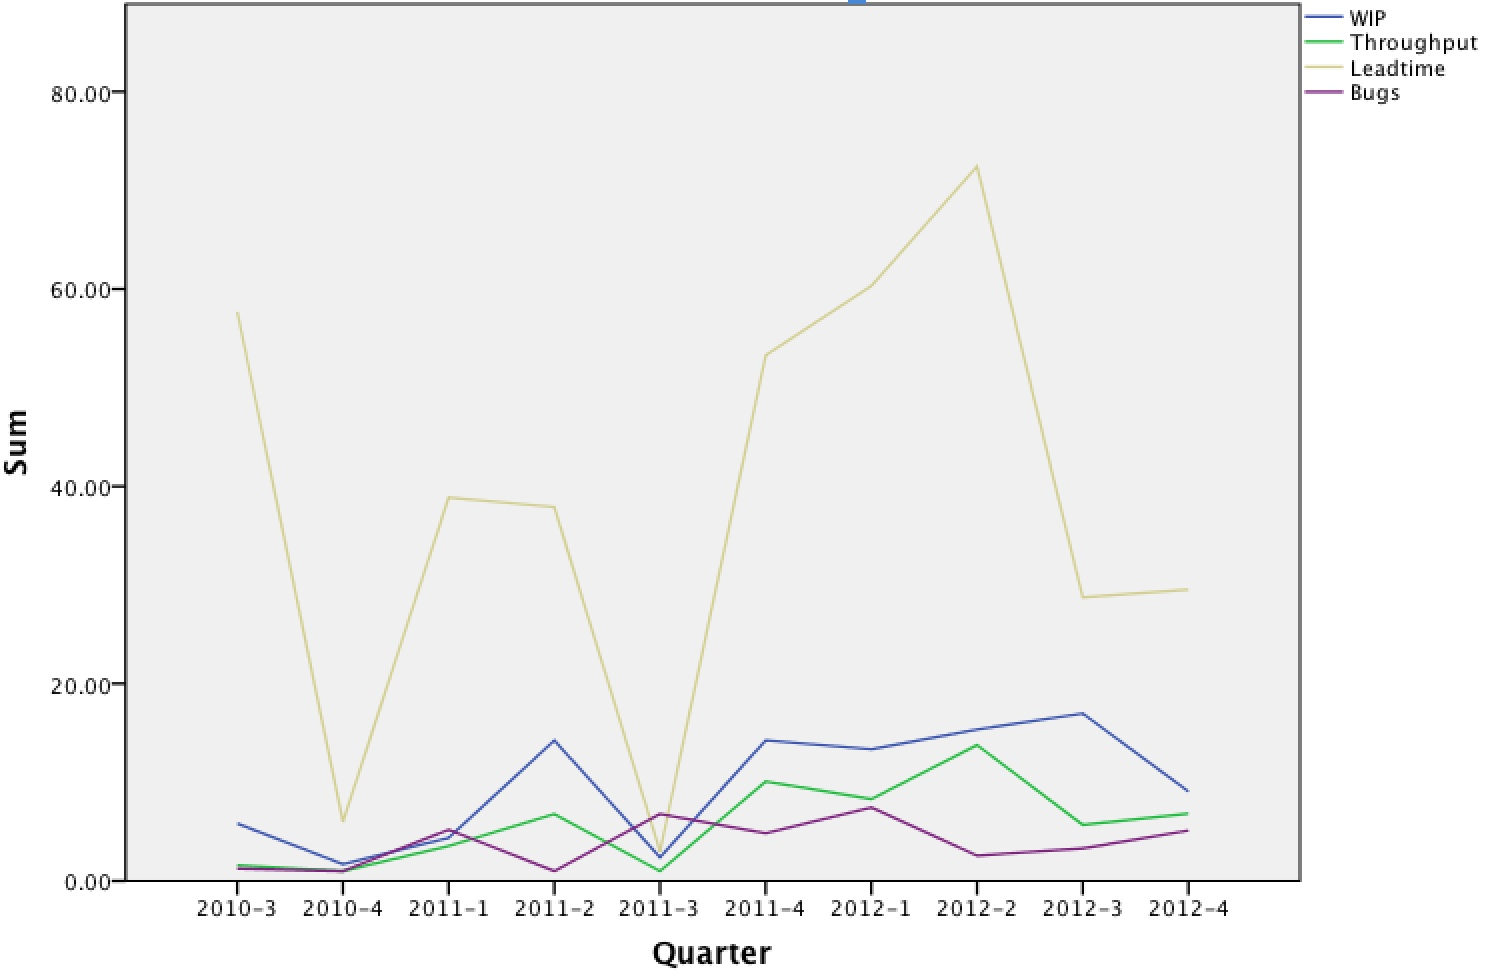
\includegraphics[scale=0.8]{Picture/360/360_WIP_TP_BUGS_LT.jpg}
\caption{WIP, Throughput, Lead time and Bugs for 360 per quarter}
\label{360pq} %% 360 per quarter
\end{figure}
\newpage

In figure \ref{Frontendpq} the average WIP, Throughput, Lead time and Bugs per quarter for team Frontend are shown
\begin{figure}[!htbp]
\centering
\hspace*{-1.2in}
\includegraphics[scale=0.7]{Picture/Frontend/Frontend-WIP-TP-LT-BUGS.jpg}
\caption{WIP, Throughput, Lead time and Bugs for Frontend per quarter}
\label{Frontendpq} %% fronted per quarter
\end{figure}
\newpage

In figure \ref{Kryptonpq} the average WIP, Throughput, Lead time and Bugs per quarter for team Krypton are shown
\begin{figure}[!htbp]
\centering
\hspace*{-1.8in}
\includegraphics[scale=0.8]{Picture/Krypton/Krypton-WIP-TP-BUGS-LT.jpg}
\caption{WIP, Throughput, Lead time and Bugs for Krypton per quarter}
\label{Kryptonpq} %% fronted per quarter
\end{figure}
\newpage


In figure \ref{Neonpq} the average WIP, Throughput, Lead time and Bugs per quarter for team Neon are shown
\begin{figure}[!htbp]
\centering
\hspace*{-1.2in}
\includegraphics[scale=1.5]{Picture/Neon/Neon-WIP-TP-BUGS-LT.jpg}
\caption{WIP, Throughput, Lead time and Bugs for Neon per quarter}
\label{Neonpq} %% fronted per quarter
\end{figure}


\chapter*{\centerline{Til Dag}}


\section {360}



  
\begin{table}[htbp]
  \centering
  \begin{adjustwidth}{-2cm}{}
  \scalebox{0.38}{
  \begin{tabular}{ | l | l | l | l | l | l | l | l | l | l | l | l | l | l | l | l | l | }
\hline
Correlations &  &  &  &  &  &  &  &  &  &  &  &  &  &  &  &  \\ \hline
	 &  & Bugs & Throughput & WIP & Churn & TP\_Feature & Churn\_Bugs & Lead time\_Union & Churn\_Union & Churn\_feature & TP\_bugs & Average\_Days\_Backlog & Bugs\_churn\_average & Average\_ft\_churn & Precent\_bugs\_fininshed & Churn\_Average \\ \hline
	Bugs & Pearson Correlation & 1 & .945** & .753* & .992** & -0.328 & .813** & -0.240 & 0.433 & .730* & .984** & 0.377 & 0.581 & 0.119 & 0.543 & 0.622\\ \hline
	 & Sig. (2-tailed) &  & 0 & 0.012 & 0 & 0.354 & 0.004 & 0.505 & 0.212 & 0.026 & 0 & 0.282 & 0.078 & 0.744 & 0.104 & 0.055\\ \hline
	 & N & 10 & 10 & 10 & 10 & 10 & 10 & 10 & 10 & 9 & 10 & 10 & 10 & 10 & 10 & 10 \\ \hline
	Throughput & Pearson Correlation & .945** & 1 & .816** & .962** & -0.340 & .776** & -0.177 & 0.399 & .736* & .940** & 0.274 & 0.626 & 0.030 & 0.420 & .638* \\ \hline
	 & Sig. (2-tailed) & 0 &  & 0.004 & 0 & 0.336 & 0.008 & 0.624 & 0.253 & 0.024 & 0 & 0.443 & 0.053 & 0.934 & 0.227 & 0.047\\ \hline
	 & N & 10 & 10 & 10 & 10 & 10 & 10 & 10 & 10 & 9 & 10 & 10 & 10 & 10 & 10 & 10 \\ \hline
	WIP & Pearson Correlation & .753* & .816** & 1 & .738* & -0.441 & .708* & -0.336 & 0.365 & 0.467 & .800** & 0.397 & 0.430 & 0.243 & 0.495 & 0.478\\ \hline
	 & Sig. (2-tailed) & 0.012 & 0.004 &  & 0.015 & 0.202 & 0.022 & 0.342 & 0.299 & 0.205 & 0.005 & 0.255 & 0.215 & 0.498 & 0.146 & 0.163\\ \hline
	 & N & 10 & 10 & 10 & 10 & 10 & 10 & 10 & 10 & 9 & 10 & 10 & 10 & 10 & 10 & 10 \\ \hline
	Churn & Pearson Correlation & .992** & .962** & .738* & 1 & -0.317 & .804** & -0.203 & 0.372 & .741* & .974** & 0.349 & 0.581 & 0.087 & 0.475 & 0.617\\ \hline
	 & Sig. (2-tailed) & 0 & 0 & 0.015 &  & 0.372 & 0.005 & 0.574 & 0.289 & 0.022 & 0 & 0.323 & 0.078 & 0.811 & 0.165 & 0.057\\ \hline
	 & N & 10 & 10 & 10 & 10 & 10 & 10 & 10 & 10 & 9 & 10 & 10 & 10 & 10 & 10 & 10 \\ \hline
	TP\_Feature & Pearson Correlation & -0.328 & -0.340 & -0.441 & -0.317 & 1 & -0.419 & 0.376 & -0.460 & -0.208 & -0.360 & 0.097 & -0.171 & -0.295 & -.795** & -0.223\\ \hline
	 & Sig. (2-tailed) & 0.354 & 0.336 & 0.202 & 0.372 &  & 0.228 & 0.284 & 0.181 & 0.591 & 0.307 & 0.789 & 0.637 & 0.408 & 0.006 & 0.536\\ \hline
	 & N & 10 & 10 & 10 & 10 & 10 & 10 & 10 & 10 & 9 & 10 & 10 & 10 & 10 & 10 & 10 \\ \hline
	Churn\_Bugs & Pearson Correlation & .813** & .776** & .708* & .804** & -0.419 & 1 & -0.126 & 0.516 & 0.597 & .884** & .700* & 0.560 & 0.523 & 0.551 & .665* \\ \hline
	 & Sig. (2-tailed) & 0.004 & 0.008 & 0.022 & 0.005 & 0.228 &  & 0.729 & 0.127 & 0.090 & 0.001 & 0.024 & 0.092 & 0.121 & 0.099 & 0.036\\ \hline
	 & N & 10 & 10 & 10 & 10 & 10 & 10 & 10 & 10 & 9 & 10 & 10 & 10 & 10 & 10 & 10 \\ \hline
	Lead time\_Union & Pearson Correlation & -0.240 & -0.177 & -0.336 & -0.203 & 0.376 & -0.126 & 1 & -0.060 & 0.138 & -0.280 & -0.012 & -0.003 & 0.158 & -0.598 & 0.059\\ \hline
	 & Sig. (2-tailed) & 0.505 & 0.624 & 0.342 & 0.574 & 0.284 & 0.729 &  & 0.868 & 0.724 & 0.433 & 0.974 & 0.994 & 0.663 & 0.068 & 0.871\\ \hline
	 & N & 10 & 10 & 10 & 10 & 10 & 10 & 10 & 10 & 9 & 10 & 10 & 10 & 10 & 10 & 10 \\ \hline
	Churn\_Union & Pearson Correlation & 0.433 & 0.399 & 0.365 & 0.372 & -0.460 & 0.516 & -0.060 & 1 & 0.202 & 0.466 & 0.231 & 0.146 & 0.410 & .634* & 0.198\\ \hline
	 & Sig. (2-tailed) & 0.212 & 0.253 & 0.299 & 0.289 & 0.181 & 0.127 & 0.868 &  & 0.603 & 0.175 & 0.522 & 0.687 & 0.239 & 0.049 & 0.584\\ \hline
	 & N & 10 & 10 & 10 & 10 & 10 & 10 & 10 & 10 & 9 & 10 & 10 & 10 & 10 & 10 & 10 \\ \hline
	Churn\_feature & Pearson Correlation & .730* & .736* & 0.467 & .741* & -0.208 & 0.597 & 0.138 & 0.202 & 1 & .681* & 0.073 & .924** & 0.008 & 0.362 & .947** \\ \hline
	 & Sig. (2-tailed) & 0.026 & 0.024 & 0.205 & 0.022 & 0.591 & 0.090 & 0.724 & 0.603 &  & 0.044 & 0.852 & 0 & 0.984 & 0.338 & 0\\ \hline
	 & N & 9 & 9 & 9 & 9 & 9 & 9 & 9 & 9 & 9 & 9 & 9 & 9 & 9 & 9 & 9 \\ \hline
	TP\_bugs & Pearson Correlation & .984** & .940** & .800** & .974** & -0.360 & .884** & -0.280 & 0.466 & .681* & 1 & 0.494 & 0.574 & 0.192 & 0.568 & 0.620\\ \hline
	 & Sig. (2-tailed) & 0 & 0 & 0.005 & 0 & 0.307 & 0.001 & 0.433 & 0.175 & 0.044 &  & 0.146 & 0.083 & 0.596 & 0.087 & 0.056\\ \hline
	 & N & 10 & 10 & 10 & 10 & 10 & 10 & 10 & 10 & 9 & 10 & 10 & 10 & 10 & 10 & 10 \\ \hline
	Average\_Days\_Backlog & Pearson Correlation & 0.377 & 0.274 & 0.397 & 0.349 & 0.097 & .700* & -0.012 & 0.231 & 0.073 & 0.494 & 1 & 0.101 & 0.595 & 0.130 & 0.217\\ \hline
	 & Sig. (2-tailed) & 0.282 & 0.443 & 0.255 & 0.323 & 0.789 & 0.024 & 0.974 & 0.522 & 0.852 & 0.146 &  & 0.782 & 0.070 & 0.721 & 0.548\\ \hline
	 & N & 10 & 10 & 10 & 10 & 10 & 10 & 10 & 10 & 9 & 10 & 10 & 10 & 10 & 10 & 10 \\ \hline
	Bugs\_churn\_average & Pearson Correlation & 0.581 & 0.626 & 0.430 & 0.581 & -0.171 & 0.560 & -0.003 & 0.146 & .924** & 0.574 & 0.101 & 1 & -0.127 & 0.322 & .973** \\ \hline
	 & Sig. (2-tailed) & 0.078 & 0.053 & 0.215 & 0.078 & 0.637 & 0.092 & 0.994 & 0.687 & 0 & 0.083 & 0.782 &  & 0.726 & 0.365 & 0\\ \hline
	 & N & 10 & 10 & 10 & 10 & 10 & 10 & 10 & 10 & 9 & 10 & 10 & 10 & 10 & 10 & 10 \\ \hline
	Average\_ft\_churn & Pearson Correlation & 0.119 & 0.030 & 0.243 & 0.087 & -0.295 & 0.523 & 0.158 & 0.410 & 0.008 & 0.192 & 0.595 & -0.127 & 1 & 0.291 & 0.088\\ \hline
	 & Sig. (2-tailed) & 0.744 & 0.934 & 0.498 & 0.811 & 0.408 & 0.121 & 0.663 & 0.239 & 0.984 & 0.596 & 0.070 & 0.726 &  & 0.415 & 0.808\\ \hline
	 & N & 10 & 10 & 10 & 10 & 10 & 10 & 10 & 10 & 9 & 10 & 10 & 10 & 10 & 10 & 10 \\ \hline
	Precent\_bugs\_fininshed & Pearson Correlation & 0.543 & 0.420 & 0.495 & 0.475 & -.795** & 0.551 & -0.598 & .634* & 0.362 & 0.568 & 0.130 & 0.322 & 0.291 & 1 & 0.369\\ \hline
	 & Sig. (2-tailed) & 0.104 & 0.227 & 0.146 & 0.165 & 0.006 & 0.099 & 0.068 & 0.049 & 0.338 & 0.087 & 0.721 & 0.365 & 0.415 &  & 0.294\\ \hline
	 & N & 10 & 10 & 10 & 10 & 10 & 10 & 10 & 10 & 9 & 10 & 10 & 10 & 10 & 10 & 10 \\ \hline
	Churn\_Average & Pearson Correlation & 0.622 & .638* & 0.478 & 0.617 & -0.223 & .665* & 0.059 & 0.198 & .947** & 0.620 & 0.217 & .973** & 0.088 & 0.369 & 1 \\ \hline
	 & Sig. (2-tailed) & 0.055 & 0.047 & 0.163 & 0.057 & 0.536 & 0.036 & 0.871 & 0.584 & 0 & 0.056 & 0.548 & 0 & 0.808 & 0.294 &  \\ \hline
	 & N & 10 & 10 & 10 & 10 & 10 & 10 & 10 & 10 & 9 & 10 & 10 & 10 & 10 & 10 & 10 \\ \hline
	 \end{tabular}
 }
  \centerline{  ** Correlation is significant at the 0.01 level (2-tailed).}
    \centerline {* Correlation is significant at the 0.05 level (2-tailed).}
      \caption{360 - Correlation}
  \label{tab:addlabelSwag}%
 \end{adjustwidth}
\end{table}%
\begin{table}[!htbp]
\centering
  \begin{adjustwidth}{-1cm}{}
     \scalebox{0.75}{
\begin{tabular}{ | l | l | l | l | l | }
\hline
	 &  &  &  &  \\ \hline
	Team & Quarter &  & Churn & Lead time \\ \hline
	360 & 2010-3 & N & 11 & 11 \\ \hline
	 &  & Mean & 17 & 3.55 \\ \hline
	 &  & Median & 11 & 3 \\ \hline
	 &  & Std. Deviation & 18.93 & 2.50 \\ \hline
	 &  & Maximum & 60 & 8 \\ \hline
	 &  & Minimum & 0 & 1 \\ \hline
	 &  &  &  &  \\ \hline
	 & 2010-4 & N & 3 & 3 \\ \hline
	 &  & Mean & 0.67 & 1.67 \\ \hline
	 &  & Median & 1 & 2 \\ \hline
	 &  & Std. Deviation & 0.57 & 0.57 \\ \hline
	 &  & Maximum & 1 & 2 \\ \hline
	 &  & Minimum & 0 & 1 \\ \hline
	 &  & N & 136 & 136 \\ \hline
	 & 2011-2 & Mean & 14.4 & 2.7 \\ \hline
	 &  & Median & 3 & 2 \\ \hline
	 &  & Std. Deviation & 21.51 & 1.85 \\ \hline
	 &  & Maximum & 83 & 8 \\ \hline
	 &  & Minimum & 0 & 1 \\ \hline
	 &  & N & 48 & 48 \\ \hline
	 & 2011-3 & Mean & 1.67 & 3.06 \\ \hline
	 &  & Median & 0 & 2.5 \\ \hline
	 &  & Std. Deviation & 7.71 & 2.13 \\ \hline
	 &  & Maximum & 50 & 8 \\ \hline
	 &  & Minimum & 0 & 1 \\ \hline
	 &  & N & 156 & 156 \\ \hline
	 & 2011-4 & Mean & 14.81 & 2.25 \\ \hline
	 &  & Median & 6.5 & 2 \\ \hline
	 &  & Std. Deviation & 19.90 & 1.53 \\ \hline
	 &  & Maximum & 86 & 8 \\ \hline
	 &  & Minimum & 0 & 1 \\ \hline
	 &  & N & 157 & 157 \\ \hline
	 & 2012-1 & Mean & 9.47 & 2.68 \\ \hline
	 &  & Median & 0 & 2 \\ \hline
	 &  & Std. Deviation & 19.54 & 1.758 \\ \hline
	 &  & Maximum & 86 & 8 \\ \hline
	 &  & Minimum & 0 & 1 \\ \hline
	 &  & N & 238 & 238 \\ \hline
	 & 2012-2 & Mean & 10.11 & 2.78 \\ \hline
	 &  & Median & 0 & 2 \\ \hline
	 &  & Std. Deviation & 18.50 & 1.597 \\ \hline
	 &  & Maximum & 83 & 8 \\ \hline
	 &  & Minimum & 0 & 1 \\ \hline
	 &  & N & 53 & 53 \\ \hline
	 & 2012-3 & Mean & 3.02 & 1.68 \\ \hline
	 &  & Median & 0 & 1 \\ \hline
	 &  & Std. Deviation & 9.61 & 1.18\\ \hline
	 &  & Maximum & 53 & 7 \\ \hline
	 &  & Minimum & 0 & 1 \\ \hline
	 &  & N & 26 & 26 \\ \hline
	 & 2012-4 & Mean & 21.42 & 2.08 \\ \hline
	 &  & Median & 14.5 & 2 \\ \hline
	 &  & Std. Deviation & 20.54 & 1.16 \\ \hline
	 &  & Maximum & 67 & 5 \\ \hline
	 &  & Minimum & 1 & 1 \\ \hline
	 &  & N & 902 & 902 \\ \hline
	 & Total & Mean & 10.14 & 2.7 \\ \hline
	 &  & Median & 0 & 2 \\ \hline
	 &  & Std. Deviation & 18.55 & 1.798 \\ \hline
	 &  & Maximum & 86 & 8 \\ \hline
	 &  & Minimum & 0 & 1 \\ \hline
\end{tabular}
}
\caption{Descriptive statistic  - Lead-time and churn - 360}
\end{adjustwidth}
 \end{table}%
 
	

 
%%%%%%%%%%%%%%%%%
\section*{Frontend} 
 \begin{table}[!htbp]
  \centering
    \begin{adjustwidth}{-2.5cm}{}
    \scalebox{0.38}{
    \begin{tabular}{ | l | l | l | l | l | l | l | l | l | l | l | l | l | l | l | l | l | }
\hline
	Correlations &  &  &  &  &  &  &  &  &  &  &  &  &  &  &  &  \\ \hline
	 &  & WIP & Throughput & Bugs & Churn & TP\_feature & Churn\_Bugs & Churn\_union & Lead time\_union & Churn\_feature & Tp\_bugs & Average\_Days\_Backlog\_Bugs & Bugs\_Churn\_average & Churn\_feature\_Average & Precent\_bugs\_fininshed & Churn\_Average \\ \hline
	WIP & Pearson Correlation & 1 & 0.491 & 0.278 & -0.446 & 0.380 & -0.446 & 0.316 & 0.096 & 0.362 & 0.508 & -0.178 & 0.257 & 0.337 & 0.367 & 0.223\\ \hline
	 & Sig. (2-tailed) &  & 0.150 & 0.436 & 0.196 & 0.279 & 0.196 & 0.373 & 0.791 & 0.304 & 0.134 & 0.622 & 0.473 & 0.341 & 0.297 & 0.537\\ \hline
	 & N & 10 & 10 & 10 & 10 & 10 & 10 & 10 & 10 & 10 & 10 & 10 & 10 & 10 & 10 & 10 \\ \hline
	Throughput & Pearson Correlation & 0.491 & 1 & .773** & -0.036 & .741* & 0.217 & -0.494 & -0.539 & -0.433 & .758* & 0.055 & 0.259 & -0.609 & .745* & -0.575\\ \hline
	 & Sig. (2-tailed) & 0.150 &  & 0.009 & 0.921 & 0.014 & 0.548 & 0.147 & 0.108 & 0.212 & 0.011 & 0.879 & 0.470 & 0.062 & 0.013 & 0.082\\ \hline
	 & N & 10 & 10 & 10 & 10 & 10 & 10 & 10 & 10 & 10 & 10 & 10 & 10 & 10 & 10 & 10 \\ \hline
	Bugs & Pearson Correlation & 0.278 & .773** & 1 & 0.259 & 0.534 & 0.398 & -0.555 & -0.581 & -0.478 & 0.271 & 0.005 & 0.296 & -0.571 & 0.498 & -0.624\\ \hline
	 & Sig. (2-tailed) & 0.436 & 0.009 &  & 0.471 & 0.111 & 0.254 & 0.096 & 0.078 & 0.162 & 0.449 & 0.988 & 0.407 & 0.085 & 0.143 & 0.054\\ \hline
	 & N & 10 & 10 & 10 & 10 & 10 & 10 & 10 & 10 & 10 & 10 & 10 & 10 & 10 & 10 & 10 \\ \hline
	Churn & Pearson Correlation & -0.446 & -0.036 & 0.259 & 1 & -0.219 & .791** & -0.522 & -0.449 & -0.517 & -0.110 & -0.174 & 0.172 & -0.485 & -0.014 & -0.471\\ \hline
	 & Sig. (2-tailed) & 0.196 & 0.921 & 0.471 &  & 0.543 & 0.006 & 0.122 & 0.192 & 0.126 & 0.762 & 0.631 & 0.634 & 0.155 & 0.970 & 0.170\\ \hline
	 & N & 10 & 10 & 10 & 10 & 10 & 10 & 10 & 10 & 10 & 10 & 10 & 10 & 10 & 10 & 10 \\ \hline
	TP\_feature & Pearson Correlation & 0.380 & .741* & 0.534 & -0.219 & 1 & 0.214 & -0.244 & -0.312 & -0.026 & 0.427 & -0.256 & -0.007 & -0.294 & .640* & -0.319\\ \hline
	 & Sig. (2-tailed) & 0.279 & 0.014 & 0.111 & 0.543 &  & 0.553 & 0.497 & 0.381 & 0.943 & 0.219 & 0.475 & 0.984 & 0.409 & 0.046 & 0.369\\ \hline
	 & N & 10 & 10 & 10 & 10 & 10 & 10 & 10 & 10 & 10 & 10 & 10 & 10 & 10 & 10 & 10 \\ \hline
	Churn\_Bugs & Pearson Correlation & -0.446 & 0.217 & 0.398 & .791** & 0.214 & 1 & -.707* & -.771** & -0.460 & 0.040 & -0.378 & -0.035 & -0.590 & 0.388 & -.689* \\ \hline
	 & Sig. (2-tailed) & 0.196 & 0.548 & 0.254 & 0.006 & 0.553 &  & 0.022 & 0.009 & 0.181 & 0.912 & 0.282 & 0.924 & 0.073 & 0.267 & 0.027\\ \hline
	 & N & 10 & 10 & 10 & 10 & 10 & 10 & 10 & 10 & 10 & 10 & 10 & 10 & 10 & 10 & 10 \\ \hline
	Churn\_union & Pearson Correlation & 0.316 & -0.494 & -0.555 & -0.522 & -0.244 & -.707* & 1 & .704* & .844** & -0.368 & -0.139 & 0.152 & .841** & -0.312 & .981** \\ \hline
	 & Sig. (2-tailed) & 0.373 & 0.147 & 0.096 & 0.122 & 0.497 & 0.022 &  & 0.023 & 0.002 & 0.296 & 0.702 & 0.674 & 0.002 & 0.379 & 0\\ \hline
	 & N & 10 & 10 & 10 & 10 & 10 & 10 & 10 & 10 & 10 & 10 & 10 & 10 & 10 & 10 & 10 \\ \hline
	Lead time\_union & Pearson Correlation & 0.096 & -0.539 & -0.581 & -0.449 & -0.312 & -.771** & .704* & 1 & 0.492 & -0.301 & 0.327 & -0.227 & 0.631 & -.697* & .766** \\ \hline
	 & Sig. (2-tailed) & 0.791 & 0.108 & 0.078 & 0.192 & 0.381 & 0.009 & 0.023 &  & 0.148 & 0.398 & 0.357 & 0.528 & 0.050 & 0.025 & 0.010\\ \hline
	 & N & 10 & 10 & 10 & 10 & 10 & 10 & 10 & 10 & 10 & 10 & 10 & 10 & 10 & 10 & 10 \\ \hline
	Churn\_feature & Pearson Correlation & 0.362 & -0.433 & -0.478 & -0.517 & -0.026 & -0.460 & .844** & 0.492 & 1 & -0.314 & -0.358 & -0.201 & .921** & -0.172 & .842** \\ \hline
	 & Sig. (2-tailed) & 0.304 & 0.212 & 0.162 & 0.126 & 0.943 & 0.181 & 0.002 & 0.148 &  & 0.377 & 0.310 & 0.579 & 0 & 0.635 & 0.002\\ \hline
	 & N & 10 & 10 & 10 & 10 & 10 & 10 & 10 & 10 & 10 & 10 & 10 & 10 & 10 & 10 & 10 \\ \hline
	Tp\_bugs & Pearson Correlation & 0.508 & .758* & 0.271 & -0.110 & 0.427 & 0.040 & -0.368 & -0.301 & -0.314 & 1 & 0.096 & 0.034 & -0.393 & 0.622 & -0.406\\ \hline
	 & Sig. (2-tailed) & 0.134 & 0.011 & 0.449 & 0.762 & 0.219 & 0.912 & 0.296 & 0.398 & 0.377 &  & 0.792 & 0.926 & 0.261 & 0.055 & 0.245\\ \hline
	 & N & 10 & 10 & 10 & 10 & 10 & 10 & 10 & 10 & 10 & 10 & 10 & 10 & 10 & 10 & 10 \\ \hline
	Average\_Days\_Backlog\_Bugs & Pearson Correlation & -0.178 & 0.055 & 0.005 & -0.174 & -0.256 & -0.378 & -0.139 & 0.327 & -0.358 & 0.096 & 1 & -0.267 & -0.272 & -0.489 & -0.035\\ \hline
	 & Sig. (2-tailed) & 0.622 & 0.879 & 0.988 & 0.631 & 0.475 & 0.282 & 0.702 & 0.357 & 0.310 & 0.792 &  & 0.456 & 0.446 & 0.151 & 0.925\\ \hline
	 & N & 10 & 10 & 10 & 10 & 10 & 10 & 10 & 10 & 10 & 10 & 10 & 10 & 10 & 10 & 10 \\ \hline
	Bugs\_Churn\_average & Pearson Correlation & 0.257 & 0.259 & 0.296 & 0.172 & -0.007 & -0.035 & 0.152 & -0.227 & -0.201 & 0.034 & -0.267 & 1 & -0.197 & 0.371 & 0.016\\ \hline
	 & Sig. (2-tailed) & 0.473 & 0.470 & 0.407 & 0.634 & 0.984 & 0.924 & 0.674 & 0.528 & 0.579 & 0.926 & 0.456 &  & 0.585 & 0.291 & 0.966\\ \hline
	 & N & 10 & 10 & 10 & 10 & 10 & 10 & 10 & 10 & 10 & 10 & 10 & 10 & 10 & 10 & 10 \\ \hline
	Churn\_feature\_Average & Pearson Correlation & 0.337 & -0.609 & -0.571 & -0.485 & -0.294 & -0.590 & .841** & 0.631 & .921** & -0.393 & -0.272 & -0.197 & 1 & -0.389 & .846** \\ \hline
	 & Sig. (2-tailed) & 0.341 & 0.062 & 0.085 & 0.155 & 0.409 & 0.073 & 0.002 & 0.050 & 0 & 0.261 & 0.446 & 0.585 &  & 0.267 & 0.002\\ \hline
	 & N & 10 & 10 & 10 & 10 & 10 & 10 & 10 & 10 & 10 & 10 & 10 & 10 & 10 & 10 & 10 \\ \hline
	Precent\_bugs\_fininshed & Pearson Correlation & 0.367 & .745* & 0.498 & -0.014 & .640* & 0.388 & -0.312 & -.697* & -0.172 & 0.622 & -0.489 & 0.371 & -0.389 & 1 & -0.445\\ \hline
	 & Sig. (2-tailed) & 0.297 & 0.013 & 0.143 & 0.970 & 0.046 & 0.267 & 0.379 & 0.025 & 0.635 & 0.055 & 0.151 & 0.291 & 0.267 &  & 0.197\\ \hline
	 & N & 10 & 10 & 10 & 10 & 10 & 10 & 10 & 10 & 10 & 10 & 10 & 10 & 10 & 10 & 10 \\ \hline
	Churn\_Average & Pearson Correlation & 0.223 & -0.575 & -0.624 & -0.471 & -0.319 & -.689* & .981** & .766** & .842** & -0.406 & -0.035 & 0.016 & .846** & -0.445 & 1 \\ \hline
	 & Sig. (2-tailed) & 0.537 & 0.082 & 0.054 & 0.170 & 0.369 & 0.027 & 0 & 0.010 & 0.002 & 0.245 & 0.925 & 0.966 & 0.002 & 0.197 &  \\ \hline
	 & N & 10 & 10 & 10 & 10 & 10 & 10 & 10 & 10 & 10 & 10 & 10 & 10 & 10 & 10 & 10 \\ \hline
\end{tabular}
    }
       \centerline{  ** Correlation is significant at the 0.01 level (2-tailed).}
    \centerline {* Correlation is significant at the 0.05 level (2-tailed).}
      \caption{Frontend Correlation}
   \end{adjustwidth}
\end{table}%

\begin{table}[!htbp]
\centering
  \begin{adjustwidth}{-1cm}{}
     \scalebox{0.75}{
\begin{tabular}{ | l | l | l | l | l | } 
\hline
	Team & Quarter &  & Lead time & Churn \\ \hline
	Frontend & 2010-3 & N & 58 & 58 \\ \hline
	 &  & Mean & 7.43 & 127.93 \\ \hline
	 &  & Median & 6 & 53.5 \\ \hline
	 &  & Std. Deviation & 5.567 & 187.011 \\ \hline
	 &  & Maximum & 22 & 1072 \\ \hline
	 &  & Minimum & 1 & 0 \\ \hline
	 & 2010-4 & N & 130 & 130 \\ \hline
	 &  & Mean & 10.32 & 158.72 \\ \hline
	 &  & Median & 4 & 14 \\ \hline
	 &  & Std. Deviation & 15.30 & 444.805 \\ \hline
	 &  & Maximum & 78 & 4308 \\ \hline
	 &  & Minimum & 1 & 0 \\ \hline
	 & 2011-1 & N & 95 & 95 \\ \hline
	 &  & Mean & 28.01 & 566.73 \\ \hline
	 &  & Median & 11 & 47 \\ \hline
	 &  & Std. Deviation & 52.183 & 3696.125 \\ \hline
	 &  & Maximum & 434 & 35917 \\ \hline
	 &  & Minimum & 1 & 0 \\ \hline
	 & 2011-2 & N & 132 & 132 \\ \hline
	 &  & Mean & 12.17 & 496.8 \\ \hline
	 &  & Median & 5 & 19 \\ \hline
	 &  & Std. Deviation & 23.548 & 3240.172 \\ \hline
	 &  & Maximum & 184 & 35956 \\ \hline
	 &  & Minimum & 1 & 0 \\ \hline
	 & 2011-3 & N & 146 & 146 \\ \hline
	 &  & Mean & 10.66 & 174.07 \\ \hline
	 &  & Median & 6 & 14 \\ \hline
	 &  & Std. Deviation & 12.577 & 655.578 \\ \hline
	 &  & Maximum & 79 & 5650 \\ \hline
	 &  & Minimum & 1 & 0 \\ \hline
	 & 2011-4 & N & 167 & 167 \\ \hline
	 &  & Mean & 9.85 & 110.98 \\ \hline
	 &  & Median & 7 & 3 \\ \hline
	 &  & Std. Deviation & 10.9 & 480.32 \\ \hline
	 &  & Maximum & 62 & 5672 \\ \hline
	 &  & Minimum & 1 & 0 \\ \hline
	 & 2012-1 & N & 188 & 188 \\ \hline
	 &  & Mean & 13.9 & 118.64 \\ \hline
	 &  & Median & 8 & 5.5 \\ \hline
	 &  & Std. Deviation & 21.92 & 568.03 \\ \hline
	 &  & Maximum & 150 & 7565 \\ \hline
	 &  & Minimum & 1 & 0 \\ \hline
	 & 2012-2 & N & 77 & 77 \\ \hline
	 &  & Mean & 22.53 & 849.42 \\ \hline
	 &  & Median & 17 & 15 \\ \hline
	 &  & Std. Deviation & 25.52 & 3575.50 \\ \hline
	 &  & Maximum & 106 & 27170 \\ \hline
	 &  & Minimum & 1 & 0 \\ \hline
	 & 2012-3 & N & 93 & 93 \\ \hline
	 &  & Mean & 13.76 & 458.92 \\ \hline
	 &  & Median & 8 & 25 \\ \hline
	 &  & Std. Deviation & 18.023 & 1272.32 \\ \hline
	 &  & Maximum & 107 & 8600 \\ \hline
	 &  & Minimum & 1 & 0 \\ \hline
	 & 2012-4 & N & 82 & 82 \\ \hline
	 &  & Mean & 8.8007 & 428.67 \\ \hline
	 &  & Median & 4 & 54 \\ \hline
	 &  & Std. Deviation & 14.978& 1178.471 \\ \hline
	 &  & Maximum & 83 & 9368 \\ \hline
	 &  & Minimum & 1 & 0 \\ \hline
	 & Total & N & 1168 & 1168 \\ \hline
	 &  & Mean & 13.35 & 305.62 \\ \hline
	 &  & Median & 7 & 15 \\ \hline
	 &  & Std. Deviation & 23.15 & 1883.16 \\ \hline
	 &  & Maximum & 434 & 35956 \\ \hline
	 &  & Minimum & 1 & 0 \\ \hline
\end{tabular}
}
\caption{Descriptive statistic  - Lead-time and churn - Frontend}
\end{adjustwidth}
 \end{table}%
 

 

 \begin{table}[!htbp]
\begin{tabular}{ | l | l | l | l | l | l | l | l | }
\hline
TeamName & Quarter & N & Mean & Median & Std. Deviation & Maximum & Minimum \\ \hline
Frontend & 2010-3 & 14 & 2.79 & 2 & 2.91 & 12 & 1 \\ \hline
	 & 2010-4 & 39 & 2 & 1 & 1.53 & 8 & 1 \\ \hline
	 & 2011-1 & 20 & 1.85 & 1 & 1.226 & 5 & 1 \\ \hline
	 & 2011-2 & 29 & 2.86 & 2 & 3.21 & 16 & 1 \\ \hline
	 & 2011-3 & 37 & 2.41 & 2 & 1.93 & 10 & 1 \\ \hline
	 & 2011-4 & 35 & 2.89 & 1 & 5.02 & 30 & 1 \\ \hline
	 & 2012-1 & 39 & 3.56 & 2 & 3.90& 23 & 1 \\ \hline
	 & 2012-2 & 31 & 1.81 & 1 & 1.4 & 7 & 1 \\ \hline
	 & 2012-3 & 24 & 2.54 & 2 & 1.79 & 7 & 1 \\ \hline
	 & 2012-4 & 14 & 2.86 & 2 & 1.79 & 7 & 1 \\ \hline
	 & Total & 282 & 2.56 & 2 & 2.895 & 30 & 1 \\ \hline
	 	 \end{tabular}
  	  \caption{Frontend - Descriptive statistic - Bugs }%
\end{table}

 \begin{table}[!htbp]
\begin{tabular}{ | l | l | l | l | l | l | l | l | }
\hline
TeamName & Quarter & N & Mean & Median & Std. Deviation & Maximum & Minimum \\ \hline
Frontend & 2010-3 & 8 & 1.25 & 1 & 0.46 & 2 & 1 \\ \hline
	 & 2010-4 & 35 & 1.63 & 1 & 0.877 & 4 & 1 \\ \hline
	 & 2011-1 & 32 & 1.53 & 1 & 0.67& 3 & 1 \\ \hline
	 & 2011-2 & 31 & 1.74 & 2 & 0.89 & 4 & 1 \\ \hline
	 & 2011-3 & 31 & 1.97 & 2 & 1.25& 6 & 1 \\ \hline
	 & 2011-4 & 28 & 1.93 & 1 & 1.94& 11 & 1 \\ \hline
	 & 2012-1 & 22 & 2.18& 1 & 2.01 & 7 & 1 \\ \hline
	 & 2012-2 & 23 & 1.48 & 1 & 1.123 & 6 & 1 \\ \hline
	 & 2012-3 & 21 & 1.48 & 1 & 0.873 & 4 & 1 \\ \hline
	 & 2012-4 & 19 & 2.47 & 2 & 1.679 & 8 & 1 \\ \hline
	 & Total & 250 & 1.78 & 1 & 1.294 & 11 & 1 \\ \hline
 	 \end{tabular}
  	  \caption{Frontend - Descriptive statistic - TP feature }%
\end{table}

 \begin{table}[!htbp]
\begin{tabular}{ | l | l | l | l | l | l | l | l | }
\hline
TeamName & Quarter & N & Mean & Median & Std. Deviation & Maximum & Minimum \\ \hline
	Frontend & 2010-3 & 15 & 2 & 2 & 1.363 & 6 & 1 \\ \hline
	 & 2010-4 & 41 & 1.98 & 2 & 1.387 & 8 & 1 \\ \hline
	 & 2011-1 & 18 & 1.33 & 1 & 0.48 & 2 & 1 \\ \hline
	 & 2011-2 & 35 & 2.50 & 2 & 2.161 & 10 & 1 \\ \hline
	 & 2011-3 & 38 & 2.18 & 2 & 1.60 & 8 & 1 \\ \hline
	 & 2011-4 & 40 & 2.6 & 2 & 2.52 & 14 & 1 \\ \hline
	 & 2012-1 & 41 & 3.44 & 3 & 2.61 & 10 & 1 \\ \hline
	 & 2012-2 & 29 & 1.9 & 1 & 1.472 & 7 & 1 \\ \hline
	 & 2012-3 & 30 & 2.13 & 1.5 & 1.69 & 8 & 1 \\ \hline
	 & 2012-4 & 25 & 2.12 & 1 & 2.10 & 10 & 1 \\ \hline
	 & Total & 312 & 2.31 & 2 & 1.982 & 14 & 1 \\ \hline
 	 \end{tabular}
  	  \caption{Frontend - Descriptive statistic - TP bugs }%
\end{table}
%%%%%%%%%%%%%%

\section{Krypton}
\begin{table}[!htbp]
  \centering
   \begin{adjustwidth}{-2.5cm}{}
    \scalebox{0.38}{
    \begin{tabular}{|l|l|l|l|l|l|l|l|l|}
    \hline
      \begin{tabular}{ | l | l | l | l | l | l | l | l | l | l | l | l | l | l | l | l | l | }
\hline
	Correlations &  &  &  &  &  &  &  &  &  &  &  &  &  &  &  &  \\ \hline
	 &  & WIP & Throughput & Bugs & Churn & TP\_feature & Churn\_Bugs & Churn\_union & Lead time\_union & Churn\_feature & Tp\_bugs & Average\_Days\_Backlog\_Bugs & Bugs\_Churn\_average & Churn\_feature\_Average & Precent\_bugs\_fininshed & Churn\_Average \\ \hline
	WIP & Pearson Correlation & 1 & 0.491 & 0.278 & -0.446 & 0.380 & -0.446 & 0.316 & 0.096 & 0.362 & 0.508 & -0.178 & 0.257 & 0.337 & 0.367 & 0.223\\ \hline
	 & Sig. (2-tailed) &  & 0.150 & 0.436 & 0.196 & 0.279 & 0.196 & 0.373 & 0.791 & 0.304 & 0.134 & 0.622 & 0.473 & 0.341 & 0.297 & 0.537\\ \hline
	 & N & 10 & 10 & 10 & 10 & 10 & 10 & 10 & 10 & 10 & 10 & 10 & 10 & 10 & 10 & 10 \\ \hline
	Throughput & Pearson Correlation & 0.491 & 1 & .773** & -0.036 & .741* & 0.217 & -0.494 & -0.539 & -0.433 & .758* & 0.055 & 0.259 & -0.609 & .745* & -0.575\\ \hline
	 & Sig. (2-tailed) & 0.150 &  & 0.009 & 0.921 & 0.014 & 0.548 & 0.147 & 0.108 & 0.212 & 0.011 & 0.879 & 0.470 & 0.062 & 0.013 & 0.082\\ \hline
	 & N & 10 & 10 & 10 & 10 & 10 & 10 & 10 & 10 & 10 & 10 & 10 & 10 & 10 & 10 & 10 \\ \hline
	Bugs & Pearson Correlation & 0.278 & .773** & 1 & 0.259 & 0.534 & 0.398 & -0.555 & -0.581 & -0.478 & 0.271 & 0.005 & 0.296 & -0.571 & 0.498 & -0.624\\ \hline
	 & Sig. (2-tailed) & 0.436 & 0.009 &  & 0.471 & 0.111 & 0.254 & 0.096 & 0.078 & 0.162 & 0.449 & 0.988 & 0.407 & 0.085 & 0.143 & 0.054\\ \hline
	 & N & 10 & 10 & 10 & 10 & 10 & 10 & 10 & 10 & 10 & 10 & 10 & 10 & 10 & 10 & 10 \\ \hline
	Churn & Pearson Correlation & -0.446 & -0.036 & 0.259 & 1 & -0.219 & .791** & -0.522 & -0.449 & -0.517 & -0.110 & -0.174 & 0.172 & -0.485 & -0.014 & -0.471\\ \hline
	 & Sig. (2-tailed) & 0.196 & 0.921 & 0.471 &  & 0.543 & 0.006 & 0.122 & 0.192 & 0.126 & 0.762 & 0.631 & 0.634 & 0.155 & 0.970 & 0.170\\ \hline
	 & N & 10 & 10 & 10 & 10 & 10 & 10 & 10 & 10 & 10 & 10 & 10 & 10 & 10 & 10 & 10 \\ \hline
	TP\_feature & Pearson Correlation & 0.380 & .741* & 0.534 & -0.219 & 1 & 0.214 & -0.244 & -0.312 & -0.026 & 0.427 & -0.256 & -0.007 & -0.294 & .640* & -0.319\\ \hline
	 & Sig. (2-tailed) & 0.279 & 0.014 & 0.111 & 0.543 &  & 0.553 & 0.497 & 0.381 & 0.943 & 0.219 & 0.475 & 0.984 & 0.409 & 0.046 & 0.369\\ \hline
	 & N & 10 & 10 & 10 & 10 & 10 & 10 & 10 & 10 & 10 & 10 & 10 & 10 & 10 & 10 & 10 \\ \hline
	Churn\_Bugs & Pearson Correlation & -0.446 & 0.217 & 0.398 & .791** & 0.214 & 1 & -.707* & -.771** & -0.460 & 0.040 & -0.378 & -0.035 & -0.590 & 0.388 & -.689* \\ \hline
	 & Sig. (2-tailed) & 0.196 & 0.548 & 0.254 & 0.006 & 0.553 &  & 0.022 & 0.009 & 0.181 & 0.912 & 0.282 & 0.924 & 0.073 & 0.267 & 0.027\\ \hline
	 & N & 10 & 10 & 10 & 10 & 10 & 10 & 10 & 10 & 10 & 10 & 10 & 10 & 10 & 10 & 10 \\ \hline
	Churn\_union & Pearson Correlation & 0.316 & -0.494 & -0.555 & -0.522 & -0.244 & -.707* & 1 & .704* & .844** & -0.368 & -0.139 & 0.152 & .841** & -0.312 & .981** \\ \hline
	 & Sig. (2-tailed) & 0.373 & 0.147 & 0.096 & 0.122 & 0.497 & 0.022 &  & 0.023 & 0.002 & 0.296 & 0.702 & 0.674 & 0.002 & 0.379 & 0\\ \hline
	 & N & 10 & 10 & 10 & 10 & 10 & 10 & 10 & 10 & 10 & 10 & 10 & 10 & 10 & 10 & 10 \\ \hline
	Lead time\_union & Pearson Correlation & 0.096 & -0.539 & -0.581 & -0.449 & -0.312 & -.771** & .704* & 1 & 0.492 & -0.301 & 0.327 & -0.227 & 0.631 & -.697* & .766** \\ \hline
	 & Sig. (2-tailed) & 0.791 & 0.108 & 0.078 & 0.192 & 0.381 & 0.009 & 0.023 &  & 0.148 & 0.398 & 0.357 & 0.528 & 0.050 & 0.025 & 0.010\\ \hline
	 & N & 10 & 10 & 10 & 10 & 10 & 10 & 10 & 10 & 10 & 10 & 10 & 10 & 10 & 10 & 10 \\ \hline
	Churn\_feature & Pearson Correlation & 0.362 & -0.433 & -0.478 & -0.517 & -0.026 & -0.460 & .844** & 0.492 & 1 & -0.314 & -0.358 & -0.201 & .921** & -0.172 & .842** \\ \hline
	 & Sig. (2-tailed) & 0.304 & 0.212 & 0.162 & 0.126 & 0.943 & 0.181 & 0.002 & 0.148 &  & 0.377 & 0.310 & 0.579 & 0 & 0.635 & 0.002\\ \hline
	 & N & 10 & 10 & 10 & 10 & 10 & 10 & 10 & 10 & 10 & 10 & 10 & 10 & 10 & 10 & 10 \\ \hline
	Tp\_bugs & Pearson Correlation & 0.508 & .758* & 0.271 & -0.110 & 0.427 & 0.040 & -0.368 & -0.301 & -0.314 & 1 & 0.096 & 0.034 & -0.393 & 0.622 & -0.406\\ \hline
	 & Sig. (2-tailed) & 0.134 & 0.011 & 0.449 & 0.762 & 0.219 & 0.912 & 0.296 & 0.398 & 0.377 &  & 0.792 & 0.926 & 0.261 & 0.055 & 0.245\\ \hline
	 & N & 10 & 10 & 10 & 10 & 10 & 10 & 10 & 10 & 10 & 10 & 10 & 10 & 10 & 10 & 10 \\ \hline
	Average\_Days\_Backlog\_Bugs & Pearson Correlation & -0.178 & 0.055 & 0.005 & -0.174 & -0.256 & -0.378 & -0.139 & 0.327 & -0.358 & 0.096 & 1 & -0.267 & -0.272 & -0.489 & -0.035\\ \hline
	 & Sig. (2-tailed) & 0.622 & 0.879 & 0.988 & 0.631 & 0.475 & 0.282 & 0.702 & 0.357 & 0.310 & 0.792 &  & 0.456 & 0.446 & 0.151 & 0.925\\ \hline
	 & N & 10 & 10 & 10 & 10 & 10 & 10 & 10 & 10 & 10 & 10 & 10 & 10 & 10 & 10 & 10 \\ \hline
	Bugs\_Churn\_average & Pearson Correlation & 0.257 & 0.259 & 0.296 & 0.172 & -0.007 & -0.035 & 0.152 & -0.227 & -0.201 & 0.034 & -0.267 & 1 & -0.197 & 0.371 & 0.016\\ \hline
	 & Sig. (2-tailed) & 0.473 & 0.470 & 0.407 & 0.634 & 0.984 & 0.924 & 0.674 & 0.528 & 0.579 & 0.926 & 0.456 &  & 0.585 & 0.291 & 0.966\\ \hline
	 & N & 10 & 10 & 10 & 10 & 10 & 10 & 10 & 10 & 10 & 10 & 10 & 10 & 10 & 10 & 10 \\ \hline
	Churn\_feature\_Average & Pearson Correlation & 0.337 & -0.609 & -0.571 & -0.485 & -0.294 & -0.590 & .841** & 0.631 & .921** & -0.393 & -0.272 & -0.197 & 1 & -0.389 & .846** \\ \hline
	 & Sig. (2-tailed) & 0.341 & 0.062 & 0.085 & 0.155 & 0.409 & 0.073 & 0.002 & 0.050 & 0 & 0.261 & 0.446 & 0.585 &  & 0.267 & 0.002\\ \hline
	 & N & 10 & 10 & 10 & 10 & 10 & 10 & 10 & 10 & 10 & 10 & 10 & 10 & 10 & 10 & 10 \\ \hline
	Precent\_bugs\_fininshed & Pearson Correlation & 0.367 & .745* & 0.498 & -0.014 & .640* & 0.388 & -0.312 & -.697* & -0.172 & 0.622 & -0.489 & 0.371 & -0.389 & 1 & -0.445\\ \hline
	 & Sig. (2-tailed) & 0.297 & 0.013 & 0.143 & 0.970 & 0.046 & 0.267 & 0.379 & 0.025 & 0.635 & 0.055 & 0.151 & 0.291 & 0.267 &  & 0.197\\ \hline
	 & N & 10 & 10 & 10 & 10 & 10 & 10 & 10 & 10 & 10 & 10 & 10 & 10 & 10 & 10 & 10 \\ \hline
	Churn\_Average & Pearson Correlation & 0.223 & -0.575 & -0.624 & -0.471 & -0.319 & -.689* & .981** & .766** & .842** & -0.406 & -0.035 & 0.016 & .846** & -0.445 & 1 \\ \hline
	 & Sig. (2-tailed) & 0.537 & 0.082 & 0.054 & 0.170 & 0.369 & 0.027 & 0 & 0.010 & 0.002 & 0.245 & 0.925 & 0.966 & 0.002 & 0.197 &  \\ \hline
	 & N & 10 & 10 & 10 & 10 & 10 & 10 & 10 & 10 & 10 & 10 & 10 & 10 & 10 & 10 & 10 \\ \hline
\end{tabular}
      \end{tabular}%
    }
    \centerline{*Correlation is significant at the 0.05 level (2-tailed).}
  \caption{Krypton - correlation}%
  \label{swag}
    \end{adjustwidth}
\end{table}%

 \begin{table}[!htbp]
\centering
  \begin{adjustwidth}{-2cm}{}
     \scalebox{0.75}{
\begin{tabular}{ | l | l | l | l | l | }
\hline
	Team & Quarter &  & Lead time & Churn \\ \hline
	Krypton & 2010-3 & N & 46 & 46 \\ \hline
	 &  & Mean & 7.89 & 159.38 \\ \hline
	 &  & Median & 3.5 & 26.5 \\ \hline
	 &  & Std. Deviation & 11.651 & 206.584 \\ \hline
	 &  & Maximum & 71 & 647 \\ \hline
	 &  & Minimum & 1 & 0 \\ \hline
	 & 2010-4 & N & 139 & 139 \\ \hline
	 &  & Mean & 7.38 & 97.7 \\ \hline
	 &  & Median & 3 & 28 \\ \hline
	 &  & Std. Deviation & 12.88 & 145.84 \\ \hline
	 &  & Maximum & 85 & 700 \\ \hline
	 &  & Minimum & 1 & 0 \\ \hline
	 & 2011-1 & N & 153 & 153 \\ \hline
	 &  & Mean & 5.83 & 71.38 \\ \hline
	 &  & Median & 2 & 17 \\ \hline
	 &  & Std. Deviation & 7.383 & 130.40\\ \hline
	 &  & Maximum & 32 & 726 \\ \hline
	 &  & Minimum & 1 & 0 \\ \hline
	 & 2011-2 & N & 51 & 51 \\ \hline
	 &  & Mean & 14.37 & 110.45 \\ \hline
	 &  & Median & 9 & 31 \\ \hline
	 &  & Std. Deviation & 16.09 & 165.053 \\ \hline
	 &  & Maximum & 90 & 719 \\ \hline
	 &  & Minimum & 1 & 0 \\ \hline
	 & 2011-3 & N & 49 & 49 \\ \hline
	 &  & Mean & 13.71 & 119.43 \\ \hline
	 &  & Median & 8 & 27 \\ \hline
	 &  & Std. Deviation & 15.97 & 159.39 \\ \hline
	 &  & Maximum & 88 & 604 \\ \hline
	 &  & Minimum & 1 & 1 \\ \hline
	 & 2011-4 & N & 66 & 66 \\ \hline
	 &  & Mean & 10.5 & 112.36 \\ \hline
	 &  & Median & 6 & 36 \\ \hline
	 &  & Std. Deviation & 11.975 & 164.935 \\ \hline
	 &  & Maximum & 57 & 675 \\ \hline
	 &  & Minimum & 1 & 1 \\ \hline
	 & 2012-1 & N & 45 & 45 \\ \hline
	 &  & Mean & 23.73 & 99.09 \\ \hline
	 &  & Median & 8 & 23 \\ \hline
	 &  & Std. Deviation & 40.47& 149.02 \\ \hline
	 &  & Maximum & 180 & 636 \\ \hline
	 &  & Minimum & 1 & 1 \\ \hline
	 & 2012-2 & N & 45 & 45 \\ \hline
	 &  & Mean & 23 & 109.07 \\ \hline
	 &  & Median & 7 & 47 \\ \hline
	 &  & Std. Deviation & 32.08 & 131.58 \\ \hline
	 &  & Maximum & 135 & 536 \\ \hline
	 &  & Minimum & 1 & 1 \\ \hline
	 & 2012-3 & N & 74 & 74 \\ \hline
	 &  & Mean & 6.92 & 82.39 \\ \hline
	 &  & Median & 3 & 37 \\ \hline
	 &  & Std. Deviation & 9.26 & 122.637 \\ \hline
	 &  & Maximum & 35 & 713 \\ \hline
	 &  & Minimum & 1 & 1 \\ \hline
	 & 2012-4 & N & 2 & 2 \\ \hline
	 &  & Mean & 1.5 & 44 \\ \hline
	 &  & Median & 1.5 & 44 \\ \hline
	 &  & Std. Deviation & 0.70 & 1.41 \\ \hline
	 &  & Maximum & 2 & 45 \\ \hline
	 &  & Minimum & 1 & 43 \\ \hline
	 & Total & N & 683 & 683 \\ \hline
	 &  & Mean & 10.55 & 98.6 \\ \hline
	 &  & Median & 4 & 29 \\ \hline
	 &  & Std. Deviation & 18.1 & 149.01 \\ \hline
	 &  & Maximum & 180 & 726 \\ \hline
	 &  & Minimum & 1 & 0 \\ \hline
\end{tabular}
 }
\caption{Descriptive statistic  - Lead-time and churn - Krypton}

\end{adjustwidth}
 \end{table}%
 
   \begin{table}[!htbp]
   \centering
 \begin{tabular}{ | l | l | l | l | l | l | l | }
\hline
	Quarter & N & Mean & Median & Std. Deviation & Maximum & Minimum \\ \hline
	2010-3 & 14.00 & 3.07 & 2.00 & 3.47 & 14.00 & 1.00\\ \hline
	2010-4 & 71.00 & 2.73 & 2.00 & 2.05 & 11.00 & 1.00\\ \hline
	2011-1 & 67.00 & 2.55 & 2.00 & 1.96 & 13.00 & 1.00\\ \hline
	2011-2 & 38.00 & 1.97 & 2.00 & 1.03 & 4.00 & 1.00\\ \hline
	2011-3 & 43.00 & 1.65 & 1.00 & 0.92 & 4.00 & 1.00\\ \hline
	2011-4 & 53.00 & 1.83 & 1.00 & 1.31 & 6.00 & 1.00\\ \hline
	2012-1 & 40.00 & 1.90 & 1.00 & 1.46 & 7.00 & 1.00\\ \hline
	2012-2 & 27.00 & 2.07 & 2.00 & 1.36 & 6.00 & 1.00\\ \hline
	2012-3 & 40.00 & 2.70 & 2.00 & 2.43 & 13.00 & 1.00\\ \hline
	2012-4 & 3.00 & 1.00 & 1.00 & 0 & 1.00 & 1.00\\ \hline
	Total & 396.00 & 2.26 & 2.00 & 1.82 & 14.00 & 1.00\\ \hline
	 \end{tabular}
  	  \caption{Frontend - Descriptive statistic - Throughput }%
\end{table}
\begin{table}[!htbp]
\begin{tabular}{ | l | l | l | l | l | l | l | l | }
\hline
TeamName & Quarter & N & Mean & Median & Std. Deviation & Maximum & Minimum \\ \hline
Krypton & 2010-3 & 25 & 14.12 & 14 & 5.093 & 27 & 9 \\ \hline
	 & 2010-4 & 92 & 23 & 23.5 & 7.819 & 48 & 12 \\ \hline
	 & 2011-1 & 90 & 14.76 & 13.5 & 5 & 26 & 6 \\ \hline
	 & 2011-2 & 91 & 12.75 & 12 & 4.64 & 22 & 3 \\ \hline
	 & 2011-3 & 92 & 17.2 & 16 & 6.476 & 32 & 8 \\ \hline
	 & 2011-4 & 92 & 17.47 & 17 & 6.32 & 30 & 4 \\ \hline
	 & 2012-1 & 91 & 14.35 & 15 & 3.911 & 24 & 7 \\ \hline
	 & 2012-2 & 91 & 16.53 & 14 & 6.03 & 34 & 10 \\ \hline
	 & 2012-3 & 92 & 23.83 & 20 & 10.387 & 43 & 7 \\ \hline
	 & 2012-4 & 67 & 1.69 & 0 & 3.016 & 11 & 0 \\ \hline
	 & Total & 823 & 16.11 & 15 & 8.43& 48 & 0 \\ \hline
\end{tabular}
\caption{Krypton - Descriptive statistic WIP}
\end{table} 	

\begin{table}[!htbp]
\begin{tabular}{ | l | l | l | l | l | l | l | l | }
\hline
TeamName & Quarter & N & Mean & Median & Std. Deviation & Maximum & Minimum \\ \hline
Krypton & 2010-3 & 17 & 1.76 & 2 & 0.83 & 3 & 1 \\ \hline
	&2010-4 & 28 & 1.71 & 1.5 & 0.85 & 4 & 1  \  \\ \hline
	 & 2011-1 & 39 & 3.1 & 2 & 2.51 & 12 & 1 \\ \hline
	 & 2011-2 & 26 & 2.04 & 2 & 1.28 & 5 & 1 \\ \hline
	 & 2011-3 & 25 & 1.64 & 1 & 1.14 & 5 & 1 \\ \hline
	 & 2011-4 & 26 & 2 & 2 & 1.35 & 7 & 1 \\ \hline
	 & 2012-1 & 26 & 1.85 & 1 & 1.617 & 9 & 1 \\ \hline
	 & 2012-2 & 19 & 2.52 & 2 & 2.48 & 11 & 1 \\ \hline
	 & 2012-3 & 31 & 2.16 & 2 & 1.44 & 6 & 1 \\ \hline
	 & Total & 241 & 2.12 & 2 & 1.69 & 12 & 1 \\ \hline
	 & 2010-3 & 20 & 2.65 & 2 & 3.54 & 17 & 1 \\ \hline
\end{tabular}
\caption{Krypton - Descriptive statistic - Bugs}
\end{table}

\begin{table}[!htbp]
\begin{tabular}{ | l | l | l | l | l | l | l | l | }
\hline
TeamName & Quarter & N & Mean & Median & Std. Deviation & Maximum & Minimum \\ \hline
Krypton & 2010-3 & 10 & 2.20 & 1.5 & 1.619 & 5 & 1 \\ \hline
	 & 2010-4 & 48 & 2.79 & 2 & 2.278 & 11 & 1 \\ \hline
	 & 2011-1 & 30 & 1.7 & 1 & 0.95 & 4 & 1 \\ \hline
	 & 2011-2 & 17 & 1.65 & 1 & 1.115 & 4 & 1 \\ \hline
	 & 2011-3 & 20 & 1.45 & 1 & 0.82& 4 & 1 \\ \hline
	 & 2011-4 & 31 & 1.48 & 1 & 0.89 & 4 & 1 \\ \hline
	 & 2012-1 & 14 & 1.71 & 1 & 1.139 & 5 & 1 \\ \hline
	 & 2012-2 & 11 & 1.73 & 1 & 0.90& 3 & 1 \\ \hline
	 & 2012-3 & 17 & 1.53 & 1 & 0.8 & 4 & 1 \\ \hline
	 & 2012-4 & 3 & 1 & 1 & 0 & 1 & 1 \\ \hline
	 & Total & 201 & 1.9 & 1 & 1.48 & 11 & 1 \\ \hline
\end{tabular}
\caption{Krypton - Descriptive statistic  - TP feature}
\end{table}

\begin{table}[!htbp]
\begin{tabular}{ | l | l | l | l | l | l | l | l | }
\hline
TeamName & Quarter & N & Mean & Median & Std. Deviation & Maximum & Minimum \\ \hline
	Krypton & 2010-3 & 6 & 3.5 & 2.5 & 3.2090& 9 & 1 \\ \hline
	 & 2010-4 & 34 & 1.76 & 2 & 0.89 & 4 & 1 \\ \hline
	 & 2011-1 & 45 & 2.67 & 2 & 2.20 & 13 & 1 \\ \hline
	 & 2011-2 & 28 & 1.68 & 2 & 0.77& 4 & 1 \\ \hline
	 & 2011-3 & 26 & 1.62 & 1 & 0.752 & 3 & 1 \\ \hline
	 & 2011-4 & 27 & 1.89 & 1 & 1.45 & 6 & 1 \\ \hline
	 & 2012-1 & 28 & 1.86 & 1 & 1.407 & 7 & 1 \\ \hline
	 & 2012-2 & 18 & 2.06 & 2 & 1.552 & 6 & 1 \\ \hline
	 & 2012-3 & 28 & 2.93 & 3 & 2.19 & 9 & 1 \\ \hline
	 & Total & 240 & 2.13 & 2 & 1.66 & 13 & 1 \\ \hline
\end{tabular}
\caption{Krypton - Descriptive statistic  - TP bugs}
\end{table}


 %%%%%%%%%%%%%%%%
\section{Neon}

\begin{table}[!htbp]
  \centering
   \begin{adjustwidth}{-2.5cm}{}
     \scalebox{0.38}{
\begin{tabular}{ | l | l | l | l | l | l | l | l | l | l | l | l | l | l | l | l | l | }
\hline
	Correlations &  &  &  &  &  &  &  &  &  &  &  &  &  &  &  &  \\ \hline
	 &  & WIP & Throughput & Bugs & Churn & TP\_feature & Churn\_Bugs & Churn\_union & Lead time\_union & Churn\_feature & Tp\_bugs & Average\_Days\_Backlog\_Bugs & Bugs\_Churn\_average & Churn\_feature\_Average & Precent\_bugs\_fininshed & Churn\_Average \\ \hline
	WIP & Pearson Correlation & 1 & 0.491 & 0.278 & -0.446 & 0.380 & -0.446 & 0.316 & 0.096 & 0.362 & 0.508 & -0.178 & 0.257 & 0.337 & 0.367 & 0.223\\ \hline
	 & Sig. (2-tailed) &  & 0.150 & 0.436 & 0.196 & 0.279 & 0.196 & 0.373 & 0.791 & 0.304 & 0.134 & 0.622 & 0.473 & 0.341 & 0.297 & 0.537\\ \hline
	 & N & 10 & 10 & 10 & 10 & 10 & 10 & 10 & 10 & 10 & 10 & 10 & 10 & 10 & 10 & 10 \\ \hline
	Throughput & Pearson Correlation & 0.491 & 1 & .773** & -0.036 & .741* & 0.217 & -0.494 & -0.539 & -0.433 & .758* & 0.055 & 0.259 & -0.609 & .745* & -0.575\\ \hline
	 & Sig. (2-tailed) & 0.150 &  & 0.009 & 0.921 & 0.014 & 0.548 & 0.147 & 0.108 & 0.212 & 0.011 & 0.879 & 0.470 & 0.062 & 0.013 & 0.082\\ \hline
	 & N & 10 & 10 & 10 & 10 & 10 & 10 & 10 & 10 & 10 & 10 & 10 & 10 & 10 & 10 & 10 \\ \hline
	Bugs & Pearson Correlation & 0.278 & .773** & 1 & 0.259 & 0.534 & 0.398 & -0.555 & -0.581 & -0.478 & 0.271 & 0.005 & 0.296 & -0.571 & 0.498 & -0.624\\ \hline
	 & Sig. (2-tailed) & 0.436 & 0.009 &  & 0.471 & 0.111 & 0.254 & 0.096 & 0.078 & 0.162 & 0.449 & 0.988 & 0.407 & 0.085 & 0.143 & 0.054\\ \hline
	 & N & 10 & 10 & 10 & 10 & 10 & 10 & 10 & 10 & 10 & 10 & 10 & 10 & 10 & 10 & 10 \\ \hline
	Churn & Pearson Correlation & -0.446 & -0.036 & 0.259 & 1 & -0.219 & .791** & -0.522 & -0.449 & -0.517 & -0.110 & -0.174 & 0.172 & -0.485 & -0.014 & -0.471\\ \hline
	 & Sig. (2-tailed) & 0.196 & 0.921 & 0.471 &  & 0.543 & 0.006 & 0.122 & 0.192 & 0.126 & 0.762 & 0.631 & 0.634 & 0.155 & 0.970 & 0.170\\ \hline
	 & N & 10 & 10 & 10 & 10 & 10 & 10 & 10 & 10 & 10 & 10 & 10 & 10 & 10 & 10 & 10 \\ \hline
	TP\_feature & Pearson Correlation & 0.380 & .741* & 0.534 & -0.219 & 1 & 0.214 & -0.244 & -0.312 & -0.026 & 0.427 & -0.256 & -0.007 & -0.294 & .640* & -0.319\\ \hline
	 & Sig. (2-tailed) & 0.279 & 0.014 & 0.111 & 0.543 &  & 0.553 & 0.497 & 0.381 & 0.943 & 0.219 & 0.475 & 0.984 & 0.409 & 0.046 & 0.369\\ \hline
	 & N & 10 & 10 & 10 & 10 & 10 & 10 & 10 & 10 & 10 & 10 & 10 & 10 & 10 & 10 & 10 \\ \hline
	Churn\_Bugs & Pearson Correlation & -0.446 & 0.217 & 0.398 & .791** & 0.214 & 1 & -.707* & -.771** & -0.460 & 0.040 & -0.378 & -0.035 & -0.590 & 0.388 & -.689* \\ \hline
	 & Sig. (2-tailed) & 0.196 & 0.548 & 0.254 & 0.006 & 0.553 &  & 0.022 & 0.009 & 0.181 & 0.912 & 0.282 & 0.924 & 0.073 & 0.267 & 0.027\\ \hline
	 & N & 10 & 10 & 10 & 10 & 10 & 10 & 10 & 10 & 10 & 10 & 10 & 10 & 10 & 10 & 10 \\ \hline
	Churn\_union & Pearson Correlation & 0.316 & -0.494 & -0.555 & -0.522 & -0.244 & -.707* & 1 & .704* & .844** & -0.368 & -0.139 & 0.152 & .841** & -0.312 & .981** \\ \hline
	 & Sig. (2-tailed) & 0.373 & 0.147 & 0.096 & 0.122 & 0.497 & 0.022 &  & 0.023 & 0.002 & 0.296 & 0.702 & 0.674 & 0.002 & 0.379 & 0\\ \hline
	 & N & 10 & 10 & 10 & 10 & 10 & 10 & 10 & 10 & 10 & 10 & 10 & 10 & 10 & 10 & 10 \\ \hline
	Lead time\_union & Pearson Correlation & 0.096 & -0.539 & -0.581 & -0.449 & -0.312 & -.771** & .704* & 1 & 0.492 & -0.301 & 0.327 & -0.227 & 0.631 & -.697* & .766** \\ \hline
	 & Sig. (2-tailed) & 0.791 & 0.108 & 0.078 & 0.192 & 0.381 & 0.009 & 0.023 &  & 0.148 & 0.398 & 0.357 & 0.528 & 0.050 & 0.025 & 0.010\\ \hline
	 & N & 10 & 10 & 10 & 10 & 10 & 10 & 10 & 10 & 10 & 10 & 10 & 10 & 10 & 10 & 10 \\ \hline
	Churn\_feature & Pearson Correlation & 0.362 & -0.433 & -0.478 & -0.517 & -0.026 & -0.460 & .844** & 0.492 & 1 & -0.314 & -0.358 & -0.201 & .921** & -0.172 & .842** \\ \hline
	 & Sig. (2-tailed) & 0.304 & 0.212 & 0.162 & 0.126 & 0.943 & 0.181 & 0.002 & 0.148 &  & 0.377 & 0.310 & 0.579 & 0 & 0.635 & 0.002\\ \hline
	 & N & 10 & 10 & 10 & 10 & 10 & 10 & 10 & 10 & 10 & 10 & 10 & 10 & 10 & 10 & 10 \\ \hline
	Tp\_bugs & Pearson Correlation & 0.508 & .758* & 0.271 & -0.110 & 0.427 & 0.040 & -0.368 & -0.301 & -0.314 & 1 & 0.096 & 0.034 & -0.393 & 0.622 & -0.406\\ \hline
	 & Sig. (2-tailed) & 0.134 & 0.011 & 0.449 & 0.762 & 0.219 & 0.912 & 0.296 & 0.398 & 0.377 &  & 0.792 & 0.926 & 0.261 & 0.055 & 0.245\\ \hline
	 & N & 10 & 10 & 10 & 10 & 10 & 10 & 10 & 10 & 10 & 10 & 10 & 10 & 10 & 10 & 10 \\ \hline
	Average\_Days\_Backlog\_Bugs & Pearson Correlation & -0.178 & 0.055 & 0.005 & -0.174 & -0.256 & -0.378 & -0.139 & 0.327 & -0.358 & 0.096 & 1 & -0.267 & -0.272 & -0.489 & -0.035\\ \hline
	 & Sig. (2-tailed) & 0.622 & 0.879 & 0.988 & 0.631 & 0.475 & 0.282 & 0.702 & 0.357 & 0.310 & 0.792 &  & 0.456 & 0.446 & 0.151 & 0.925\\ \hline
	 & N & 10 & 10 & 10 & 10 & 10 & 10 & 10 & 10 & 10 & 10 & 10 & 10 & 10 & 10 & 10 \\ \hline
	Bugs\_Churn\_average & Pearson Correlation & 0.257 & 0.259 & 0.296 & 0.172 & -0.007 & -0.035 & 0.152 & -0.227 & -0.201 & 0.034 & -0.267 & 1 & -0.197 & 0.371 & 0.016\\ \hline
	 & Sig. (2-tailed) & 0.473 & 0.470 & 0.407 & 0.634 & 0.984 & 0.924 & 0.674 & 0.528 & 0.579 & 0.926 & 0.456 &  & 0.585 & 0.291 & 0.966\\ \hline
	 & N & 10 & 10 & 10 & 10 & 10 & 10 & 10 & 10 & 10 & 10 & 10 & 10 & 10 & 10 & 10 \\ \hline
	Churn\_feature\_Average & Pearson Correlation & 0.337 & -0.609 & -0.571 & -0.485 & -0.294 & -0.590 & .841** & 0.631 & .921** & -0.393 & -0.272 & -0.197 & 1 & -0.389 & .846** \\ \hline
	 & Sig. (2-tailed) & 0.341 & 0.062 & 0.085 & 0.155 & 0.409 & 0.073 & 0.002 & 0.050 & 0 & 0.261 & 0.446 & 0.585 &  & 0.267 & 0.002\\ \hline
	 & N & 10 & 10 & 10 & 10 & 10 & 10 & 10 & 10 & 10 & 10 & 10 & 10 & 10 & 10 & 10 \\ \hline
	Precent\_bugs\_fininshed & Pearson Correlation & 0.367 & .745* & 0.498 & -0.014 & .640* & 0.388 & -0.312 & -.697* & -0.172 & 0.622 & -0.489 & 0.371 & -0.389 & 1 & -0.445\\ \hline
	 & Sig. (2-tailed) & 0.297 & 0.013 & 0.143 & 0.970 & 0.046 & 0.267 & 0.379 & 0.025 & 0.635 & 0.055 & 0.151 & 0.291 & 0.267 &  & 0.197\\ \hline
	 & N & 10 & 10 & 10 & 10 & 10 & 10 & 10 & 10 & 10 & 10 & 10 & 10 & 10 & 10 & 10 \\ \hline
	Churn\_Average & Pearson Correlation & 0.223 & -0.575 & -0.624 & -0.471 & -0.319 & -.689* & .981** & .766** & .842** & -0.406 & -0.035 & 0.016 & .846** & -0.445 & 1 \\ \hline
	 & Sig. (2-tailed) & 0.537 & 0.082 & 0.054 & 0.170 & 0.369 & 0.027 & 0 & 0.010 & 0.002 & 0.245 & 0.925 & 0.966 & 0.002 & 0.197 &  \\ \hline
	 & N & 10 & 10 & 10 & 10 & 10 & 10 & 10 & 10 & 10 & 10 & 10 & 10 & 10 & 10 & 10 \\ \hline
\end{tabular}
    }
    \centerline{* Correlation is significant at the 0.05 level (2-tailed).}
    \centerline{** Correlation is significant at the 0.01 level (2-tailed).}
      \caption{Neon - Correlation}
      \end{adjustwidth}
\end{table}%

\begin{table}[!htbp]
\centering
  \begin{adjustwidth}{-2cm}{}
     \scalebox{0.75}{
 \begin{tabular}{ | l | l | l | l | l | }
\hline
	Team & Quarter &  & Churn & Lead time \\ \hline
	Neon & 2010-3 & N & 62 & 62 \\ \hline
	 &  & Mean & 25.27 & 7.69 \\ \hline
	 &  & Median & 9 & 6 \\ \hline
	 &  & Std. Deviation & 39.448 & 6.88 \\ \hline
	 &  & Maximum & 193 & 24 \\ \hline
	 &  & Minimum & 0 & 1 \\ \hline
	 & 2010-4 & N & 125 & 125 \\ \hline
	 &  & Mean & 33.13 & 6.66 \\ \hline
	 &  & Median & 15 & 5 \\ \hline
	 &  & Std. Deviation & 47.46 & 6.01 \\ \hline
	 &  & Maximum & 214 & 27 \\ \hline
	 &  & Minimum & 0 & 1 \\ \hline
	 & 2011-1 & N & 132 & 132 \\ \hline
	 &  & Mean & 23.81 & 6.53 \\ \hline
	 &  & Median & 9 & 5.5 \\ \hline
	 &  & Std. Deviation & 41.22 & 5.43 \\ \hline
	 &  & Maximum & 301 & 27 \\ \hline
	 &  & Minimum & 0 & 1 \\ \hline
	 & 2011-2 & N & 134 & 134 \\ \hline
	 &  & Mean & 36.1 & 10.71 \\ \hline
	 &  & Median & 7 & 6 \\ \hline
	 &  & Std. Deviation & 59.067 & 35.19 \\ \hline
	 &  & Maximum & 271 & 408 \\ \hline
	 &  & Minimum & 0 & 1 \\ \hline
	 & 2011-3 & N & 99 & 99 \\ \hline
	 &  & Mean & 40.86 & 8.34 \\ \hline
	 &  & Median & 17 & 6 \\ \hline
	 &  & Std. Deviation & 50.60 & 6.61 \\ \hline
	 &  & Maximum & 239 & 27 \\ \hline
	 &  & Minimum & 1 & 1 \\ \hline
	 & 2011-4 & N & 98 & 98 \\ \hline
	 &  & Mean & 63.31 & 8.5 \\ \hline
	 &  & Median & 38 & 7 \\ \hline
	 &  & Std. Deviation & 74.35 & 6.84 \\ \hline
	 &  & Maximum & 294 & 27 \\ \hline
	 &  & Minimum & 1 & 1 \\ \hline
	 & 2012-1 & N & 110 & 110 \\ \hline
	 &  & Mean & 56.75 & 5.16 \\ \hline
	 &  & Median & 21 & 4 \\ \hline
	 &  & Std. Deviation & 72.52 & 4.46 \\ \hline
	 &  & Maximum & 296 & 22 \\ \hline
	 &  & Minimum & 1 & 1 \\ \hline
	 & 2012-2 & N & 81 & 81 \\ \hline
	 &  & Mean & 44.95 & 5.05 \\ \hline
	 &  & Median & 22 & 4 \\ \hline
	 &  & Std. Deviation & 54.23 & 4.43 \\ \hline
	 &  & Maximum & 300 & 23 \\ \hline
	 &  & Minimum & 1 & 1 \\ \hline
	 & 2012-3 & N & 174 & 174 \\ \hline
	 &  & Mean & 66.12 & 5.78 \\ \hline
	 &  & Median & 33.5 & 4 \\ \hline
	 &  & Std. Deviation & 81.02 & 4.35\\ \hline
	 &  & Maximum & 299 & 21 \\ \hline
	 &  & Minimum & 1 & 1 \\ \hline
	 & 2012-4 & N & 120 & 120 \\ \hline
	 &  & Mean & 75.930000000000007 & 5.3 \\ \hline
	 &  & Median & 32 & 4.5 \\ \hline
	 &  & Std. Deviation & 86.49 & 4. \\ \hline
	 &  & Maximum & 303 & 17 \\ \hline
	 &  & Minimum & 1 & 1 \\ \hline
	 & Total & N & 1155 & 1155 \\ \hline
	 &  & Mean & 47.76 & 7 \\ \hline
	 &  & Median & 18 & 5 \\ \hline
	 &  & Std. Deviation & 66.37 & 13.112 \\ \hline
	 &  & Maximum & 303 & 408 \\ \hline
	 &  & Minimum & 0 & 1 \\ \hline
\end{tabular}
}
\caption{Descriptive statistic  - Lead-time and churn - Neon}

\end{adjustwidth}
 \end{table}%
 
   \begin{table}[!htbp]
\begin{tabular}{ | l | l | l | l | l | l | l | l | }
\hline
Team & Quarter & N & Mean & Median & Std. Deviation & Maximum & Minimum \\ \hline
 Neon & 2010-3 & 10 & 2 & 1.5 & 1.333 & 5 & 1 \\ \hline
	 & 2010-4 & 34 & 1.68 & 1 & 1.173 & 6 & 1 \\ \hline
	 & 2011-1 & 31 & 1.71 & 1 & 1.03 & 5 & 1 \\ \hline
	 & 2011-2 & 6 & 1.17 & 1 & 0.4 & 2 & 1 \\ \hline
	 & 2011-3 & 9 & 1 & 1 & 0 & 1 & 1 \\ \hline
	 & 2011-4 & 1 & 1 & 1 & . & 1 & 1 \\ \hline
	 & Total & 91 & 1.62 & 1 & 1.06 & 6 & 1 \\ \hline
\end{tabular}
\caption{Neon - Descriptive statistic - Throughput}
\end{table}
 
\begin{table}[!htbp]
\begin{tabular}{ | l | l | l | l | l | l | l | l | }
\hline
TeamName & Quarter & N & Mean & Median & Std. Deviation & Maximum & Minimum \\ \hline
Neon & 2010-3 & 25 & 14.4 & 15 & 6.19 & 23 & 6 \\ \hline
	 & 2010-4 & 92 & 21.41 & 20 & 7.17 & 41 & 9 \\ \hline
	 & 2011-1 & 90 & 27.2 & 27.5 & 4.90 & 38 & 17 \\ \hline
	 & 2011-2 & 91 & 29.71 & 27 & 14.42 & 62 & 12 \\ \hline
	 & 2011-3 & 92 & 31.98 & 30 & 8.90 & 55 & 18 \\ \hline
	 & 2011-4 & 92 & 29.09 & 29 & 10.09 & 45 & 12 \\ \hline
	 & 2012-1 & 91 & 19.03 & 18 & 4.63 & 30 & 7 \\ \hline
	 & 2012-2 & 91 & 24.34 & 25 & 10.282 & 50 & 5 \\ \hline
	 & 2012-3 & 92 & 23.24 & 21.5 & 7.89 & 44 & 10 \\ \hline
	 & 2012-4 & 92 & 19.48 & 22 & 10.99 & 45 & 1 \\ \hline
	 & 2013-1 & 11 & 2.18& 2 & 0.60 & 3 & 1 \\ \hline
	 & Total & 859 & 24.45 & 24 & 10.54& 62 & 1 \\ \hline
\end{tabular}
\caption{Neon - Descriptive statistic - WIP}
\end{table}

\begin{table}[!htbp]
\begin{tabular}{ | l | l | l | l | l | l | l | l | }
\hline
	TeamName & Quarter & N & Mean & Median & Std. Deviation & Maximum & Minimum \\ \hline
	Neon & 2010-4 & 40 & 2.45& 2 & 1.694 & 9 & 1 \\ \hline
	 & 2011-1 & 47 & 2.43 & 2 & 1.80& 8 & 1 \\ \hline
	 & 2011-2 & 42 & 3.57 & 3 & 2.52 & 13 & 1 \\ \hline
	&2011-3 & 45 & 2.47 & 2 & 2.33 & 13 & 1  \  \\ \hline
	 & 2011-4 & 48 & 2.48 & 2 & 1.59 & 7 & 1 \\ \hline
	 & 2012-1 & 36 & 3.25 & 3 & 3.03& 16 & 1 \\ \hline
	 & 2012-2 & 36 & 2.19 & 2 & 1.48 & 8 & 1 \\ \hline
	 & 2012-3 & 44 & 3.43 & 2 & 2.55 & 10 & 1 \\ \hline
	 & 2012-4 & 33 & 3.12 & 2 & 2.63& 10 & 1 \\ \hline
	 & 2013-1 & 1 & 1 & 1 & . & 1 & 1 \\ \hline
	 & Total & 404 & 2.75 & 2 & 2.306 & 17 & 1 \\ \hline
\end{tabular}
\caption{Neon - Descriptive statistic - Bugs}
\end{table}

\begin{table}[!htbp]
\begin{tabular}{ | l | l | l | l | l | l | l | l | }
\hline
	TeamName & Quarter & N & Mean & Median & Std. Deviation & Maximum & Minimum \\ \hline
	Neon & 2010-3 & 10 & 2 & 1.5 & 1.333 & 5 & 1 \\ \hline
	 & 2010-4 & 34 & 1.68 & 1 & 1.173 & 6 & 1 \\ \hline
	 & 2011-1 & 31 & 1.71 & 1 & 1.038 & 5 & 1 \\ \hline
	 & 2011-2 & 11 & 1.27 & 1 & 0.64 & 3 & 1 \\ \hline
	 & 2011-3 & 34 & 1.53 & 1 & 0.99 & 5 & 1 \\ \hline
	 & 2011-4 & 16 & 1.5 & 1 & 0.73 & 3 & 1 \\ \hline
	 & 2012-1 & 23 & 1.3 & 1 & 0.70 & 4 & 1 \\ \hline
	 & 2012-2 & 32 & 1.63 & 1 & 0.83 & 4 & 1 \\ \hline
	 & 2012-3 & 32 & 2.02& 2 & 0.93 & 4 & 1 \\ \hline
	 & 2012-4 & 40 & 1.93 & 2 & 1.11 & 6 & 1 \\ \hline
	 & Total & 263 & 1.69 & 1 & 0.997 & 6 & 1 \\ \hline
\end{tabular}
\caption{Neon - Descriptive statistic - TP feature}
\end{table}

\begin{table}[!htbp]
\begin{tabular}{ | l | l | l | l | l | l | l | l | }
\hline
	TeamName & Quarter & N & Mean & Median & Std. Deviation & Maximum & Minimum \\ \hline
	Neon & 2010-3 & 10 & 2 & 1.5 & 1.333 & 5 & 1 \\ \hline
	 & 2010-4 & 34 & 1.68 & 1 & 1.173 & 6 & 1 \\ \hline
	 & 2011-1 & 31 & 1.71 & 1 & 1.038 & 5 & 1 \\ \hline
	 & 2011-2 & 11 & 1.27 & 1 & 0.64 & 3 & 1 \\ \hline
	 & 2011-3 & 34 & 1.53 & 1 & 0.99 & 5 & 1 \\ \hline
	 & 2011-4 & 16 & 1.5 & 1 & 0.73 & 3 & 1 \\ \hline
	 & 2012-1 & 23 & 1.3 & 1 & 0.70 & 4 & 1 \\ \hline
	 & 2012-2 & 32 & 1.63 & 1 & 0.83 & 4 & 1 \\ \hline
	 & 2012-3 & 32 & 2.02& 2 & 0.93& 4 & 1 \\ \hline
	 & 2012-4 & 40 & 1.93 & 2 & 1.11 & 6 & 1 \\ \hline
	 & Total & 263 & 1.69 & 1 & 0.997 & 6 & 1 \\ \hline
\end{tabular}
\caption{Neon - Descriptive statistic - TP bugs}
\end{table}


\chapter{Conclusion}
\label{ch:con}


\backmatter{}
\printbibliography
\end{document}
